%%%%%%%%%%%%%%%%%%%%%%%%%%%%%%%%%%%%%%%%%%%%%%%%%%%%%%%%%%%%%%%%%%%%%%%%%%%%%
%%%%%%%%% Very basic document style settings %%%%%%%%%
\documentclass[handout]{beamer}
\usetheme{Madrid}
\usefonttheme{professionalfonts}
\setbeamertemplate{itemize items}[triangle]
\setbeamertemplate{section in toc}[ball]
%%%%%%%%%%%%%%%%%%%%%%%%%%%%%%%%%%%%%%%%%%%%%%%%%%%%%%%%%%%%%%%%%%%%%%%%%%%%%

%%%%%%%%%%%%%%%%%%%%%%%%%%%%%%%%%%%%%%%%%%%%%%%%%%%%%%%%%%%%%%%%%%%%%%%%%%%%%
%%%%%%%%% logo & author information for the entire slide set %%%%%%%%%
\titlegraphic{\href{https://ei.uni-paderborn.de/lea/}{
\includegraphics[height=1cm]{fig/UPB_Logo}}\hspace{2cm} \href{https://creativecommons.org/licenses/by-nc-sa/4.0/legalcode}{
\includegraphics[height=1cm]{fig/by-nc-sa}}}
\author{Oliver Wallscheid}
%%%%%%%%%%%%%%%%%%%%%%%%%%%%%%%%%%%%%%%%%%%%%%%%%%%%%%%%%%%%%%%%%%%%%%%%%%%%%


%%%%%%%%%%%%%%%%%%%%%%%%%%%%%%%%%%%%%%%%%%%%%%%%%%%%%%%%%%%%%%%%%%%%%%%%%%%%%
%%%%%%%%% Basic packages %%%%%%%%%
\usepackage[boxed, noend, noline]{algorithm2e}
\usepackage[ansinew]{inputenc}
\usepackage{amsmath}
\usepackage{amsfonts}
\usepackage{subfig}
\usepackage{ragged2e}
\usepackage{array}
\usepackage{hhline}
\usepackage{units}
\usepackage{color}
\usepackage{bm}
\usepackage{animate}
\usepackage{multirow}
\definecolor{links}{HTML}{2A1B81}
\hypersetup{colorlinks,linkcolor=,urlcolor=links}
\usepackage[font=small,justification=centering]{caption}
%%%%%%%%%%%%%%%%%%%%%%%%%%%%%%%%%%%%%%%%%%%%%%%%%%%%%%%%%%%%%%%%%%%%%%%%%%%%%

%%%%%%%%%%%%%%%%%%%%%%%%%%%%%%%%%%%%%%%%%%%%%%%%%%%%%%%%%%%%%%%%%%%%%%%%%%%%%
%%%% Include creative commons license to pdf footrpint %%%%%
\usepackage{xmpincl}
\includexmp{CC}
%%%%%%%%%%%%%%%%%%%%%%%%%%%%%%%%%%%%%%%%%%%%%%%%%%%%%%%%%%%%%%%%%%%%%%%%%%%%%

%%%%%%%%%%%%%%%%%%%%%%%%%%%%%%%%%%%%%%%%%%%%%%%%%%%%%%%%%%%%%%%%%%%%%%%%%%%%%
%%%% Warning handlings %%%%%
\pdfsuppresswarningpagegroup=1 %Due to a bug in pdflatex one recieves an unuseful warning "pdf inclusion: multiple pdfs with page group included in a single page" if multiple pdfs (e.g. figures from Inkscape) are inserted into one frame.
%%%%%%%%%%%%%%%%%%%%%%%%%%%%%%%%%%%%%%%%%%%%%%%%%%%%%%%%%%%%%%%%%%%%%%%%%%%%%

%%%%%%%%%%%%%%%%%%%%%%%%%%%%%%%%%%%%%%%%%%%%%%%%%%%%%%%%%%%%%%%%%%%%%%%%%%%%%
%%%% Color Definitions %%%%%
\definecolor{uniblau}{rgb}{0.2,0.2,0.7}
\definecolor{unigrey}{rgb}{0.85,0.85,0.85}
\newcommand{\hl}[1]{\textcolor{red}{#1}} %Highlights in text
\newcommand{\hlh}[1]{\textbf{#1}} %Highlights in sub-headings
%%%%%%%%%%%%%%%%%%%%%%%%%%%%%%%%%%%%%%%%%%%%%%%%%%%%%%%%%%%%%%%%%%%%%%%%%%%%%

%%%%%%%%%%%%%%%%%%%%%%%%%%%%%%%%%%%%%%%%%%%%%%%%%%%%%%%%%%%%%%%%%%%%%%%%%%%%%
%%%% New footnote comamand without numbering %%%%%
\newcommand\blfootnote[1]{%
  \begingroup
  \renewcommand\thefootnote{}\footnote{#1}%
  \addtocounter{footnote}{-1}%
  \endgroup
}
%%%%%%%%%%%%%%%%%%%%%%%%%%%%%%%%%%%%%%%%%%%%%%%%%%%%%%%%%%%%%%%%%%%%%%%%%%%%%

%%%%%%%%%%%%%%%%%%%%%%%%%%%%%%%%%%%%%%%%%%%%%%%%%%%%%%%%%%%%%%%%%%%%%%%%%%%%%
%%%% check- and x-mark %%%%%
\usepackage{pifont}% http://ctan.org/pkg/pifont
\newcommand{\cmark}{\ding{51}}%
\newcommand{\xmark}{\ding{55}}%
%%%%%%%%%%%%%%%%%%%%%%%%%%%%%%%%%%%%%%%%%%%%%%%%%%%%%%%%%%%%%%%%%%%%%%%%%%%%%

%%%%%%%%%%%%%%%%%%%%%%%%%%%%%%%%%%%%%%%%%%%%%%%%%%%%%%%%%%%%%%%%%%%%%%%%%%%%%
%%%% Centered p-box & m-box in table env. using array package %%%%%
\newcolumntype{P}[1]{>{\centering\arraybackslash}p{#1}}
\newcolumntype{M}[1]{>{\centering\arraybackslash}m{#1}}
%%%%%%%%%%%%%%%%%%%%%%%%%%%%%%%%%%%%%%%%%%%%%%%%%%%%%%%%%%%%%%%%%%%%%%%%%%%%%

%%%%%%%%%%%%%%%%%%%%%%%%%%%%%%%%%%%%%%%%%%%%%%%%%%%%%%%%%%%%%%%%%%%%%%%%%%%%%
%%%% Blocks %%%%%
\usepackage[listings,theorems]{tcolorbox}
\usepackage{tikz}

%Math. definitions
\newcounter{mydefi}[section]
\def\themydefi{\arabic{part}.\arabic{mydefi}}
\tcbmaketheorem{defi}{Definition}{grow to left by=0.15cm, grow to right by=0.15cm, left=0.05cm, right=0.05cm,bottom=0.05cm, top=0.05cm,arc=1mm, colback=block body.bg,colframe = block title.bg}{mydefi}{defi}		

%Math. theorems		
\newcounter{mytheo}[section]
\def\themytheo{\arabic{part}.\arabic{mytheo}}
\tcbmaketheorem{theo}{Theorem}{grow to left by=0.15cm, grow to right by=0.15cm, left=0.05cm, right=0.05cm,bottom=0.05cm, top=0.05cm,arc=1mm, colback=block body.bg,colframe = block title.bg}{mytheo}{theo}

%Algorithms	
\newcounter{myalgo}[section]
\def\themyalgo{\arabic{part}.\arabic{myalgo}}
\tcbmaketheorem{algo}{Algorithm}{grow to left by=0.15cm, grow to right by=0.15cm, left=0.05cm, right=0.05cm,bottom=0.05cm, top=0.05cm,arc=1mm, colback=block body.bg,colframe = block title.bg}{myalgo}{algo}

%%%%%%%%%%%%%%%%%%%%%%%%%%%%%%%%%%%%%%%%%%%%%%%%%%%%%%%%%%%%%%%%%%%%%%%%%%%%%%

%%%%%%%%%%%%%%%%%%%%%%%%%%%%%%%%%%%%%%%%%%%%%%%%%%%%%%%%%%%%%%%%%%%%%%%%%%%%%
%%%% Font definition for algorithm caption  %%%%%
\SetAlCapFnt{\normalfont\color{uniblau}}
%%%%%%%%%%%%%%%%%%%%%%%%%%%%%%%%%%%%%%%%%%%%%%%%%%%%%%%%%%%%%%%%%%%%%%%%%%%%%

%%%%%%%%%%%%%%%%%%%%%%%%%%%%%%%%%%%%%%%%%%%%%%%%%%%%%%%%%%%%%%%%%%%%%%%%%%%%%
%%%% Ensure that section numbering per part is starting at one   %%%%%
\makeatletter
\AtBeginPart{%
 \beamer@tocsectionnumber=0\relax
  \setcounter{section}{0}
	\setcounter{framenumber}{0}
	\setcounter{mytheo}{0}
	\setcounter{mydefi}{0}
}
\makeatother
%%%%%%%%%%%%%%%%%%%%%%%%%%%%%%%%%%%%%%%%%%%%%%%%%%%%%%%%%%%%%%%%%%%%%%%%%%%%%

%%%%%%%%%%%%%%%%%%%%%%%%%%%%%%%%%%%%%%%%%%%%%%%%%%%%%%%%%%%%%%%%%%%%%%%%%%%%%
%%%% Delete absolute page number depiction since \inserttotalframenumber is not updated to zero when using \part command  %%%%%
\makeatletter
\setbeamertemplate{footline}{
  \leavevmode%
  \hbox{%
  \begin{beamercolorbox}[wd=.333333\paperwidth,ht=2.25ex,dp=1ex,center]{author in head/foot}%
    \usebeamerfont{author in head/foot}\insertshortauthor\expandafter\ifblank\expandafter{\beamer@shortinstitute}{}{~~(\insertshortinstitute)}
  \end{beamercolorbox}%
  \begin{beamercolorbox}[wd=.333333\paperwidth,ht=2.25ex,dp=1ex,center]{title in head/foot}%
    \usebeamerfont{title in head/foot}\insertshorttitle
  \end{beamercolorbox}%
  \begin{beamercolorbox}[wd=.333333\paperwidth,ht=2.25ex,dp=1ex,right]{date in head/foot}%
    \usebeamerfont{date in head/foot}\insertshortdate{}\hspace*{5em}
    \insertframenumber{}%/\inserttotalframenumber
    \hspace*{2ex} 
  \end{beamercolorbox}}%
  \vskip0pt%

}
\makeatother
%%%%%%%%%%%%%%%%%%%%%%%%%%%%%%%%%%%%%%%%%%%%%%%%%%%%%%%%%%%%%%%%%%%%%%%%%%%%%

%%%%%%%%%%%%%%%%%%%%%%%%%%%%%%%%%%%%%%%%%%%%%%%%%%%%%%%%%%%%%%%%%%%%%%%%%%%%%
%%%% References %%%%%
\newcommand{\figref}[1]{\figurename~\ref{#1}}
\newcommand{\satzref}[1]{Theo.~\ref{#1}}
\newcommand{\defref}[1]{Def.~\ref{#1}}
\newcommand{\theoref}[1]{Theo.~\ref{#1}}
\newcommand{\tabref}[1]{\tablename~\ref{#1}}
\newcommand{\capref}[1]{\capname~\ref{#1}}
\newcommand{\apref}[1]{\apname~\ref{#1}}
\newcommand{\algname}{Algo.}
\newcommand{\algoref}[1]{\algname~\ref{#1}}
\setbeamertemplate{caption}{\raggedright\centering\insertcaption\par}
%%%%%%%%%%%%%%%%%%%%%%%%%%%%%%%%%%%%%%%%%%%%%%%%%%%%%%%%%%%%%%%%%%%%%%%%%%%%%%

%%%%%%%%%%%%%%%%%%%%%%%%%%%%%%%%%%%%%%%%%%%%%%%%%%%%%%%%%%%%%%%%%%%%%%%%%%%%%
%%%% Numbering of captions  %%%%%
\setbeamertemplate{caption}[numbered] %Gives basic numbering to captions
\numberwithin{figure}{part} %Allows for \part.\figure style numbering
\renewcommand\figurename{Fig.}
\numberwithin{equation}{part} %Allows for \part.\equation style numbering
\numberwithin{table}{part} %Allows for \part.\table style numbering
\renewcommand\tablename{Tab.}
\renewcommand{\algorithmcfname}{Algo.} %Algorithm-Name
\numberwithin{algocf}{part} %Allows for \part.\algo style numbering
%%%%%%%%%%%%%%%%%%%%%%%%%%%%%%%%%%%%%%%%%%%%%%%%%%%%%%%%%%%%%%%%%%%%%%%%%%%%%



%%%%%%%%%%%%%%%%%%%%%%%%%%%%%%%%%%%%%%%%%%%%%%%%%%%%%%%%%%%%%%%%%%%%%%%%%%%%%
%%%% Math short commands  %%%%%
\newcommand{\E}[1]{\mathbb{E}\left[#1\right]} %Expected value
\newcommand{\Var}[1]{\mathrm{Var}\left[#1\right]} %Variance value
\newcommand{\El}[2]{\mathbb{E}_{#2}\left[#1\right]} %Expected value with lower index
\newcommand{\Pb}[1]{\mathbb{P}\left[#1\right]} %Propability
\newcommand{\T}{^{\mkern-1.5mu\mathsf{T}}} %Transpose
\DeclareMathOperator*{\argmax}{arg\,max} % arg max
\DeclareMathOperator*{\argmin}{arg\,min} % arg min
%%%%%%%%%%%%%%%%%%%%%%%%%%%%%%%%%%%%%%%%%%%%%%%%%%%%%%%%%%%%%%%%%%%%%%%%%%%%%

%%%%%%%%%%%%%%%%%%%%%%%%%%%%%%%%%%%%%%%%%%%%%%%%%%%%%%%%%%%%%%%%%%%%%%%%%%%%%
%%%% Ohter useful short commands  %%%%%
\newcommand{\SilverLectureSource}{(source: D. Silver, Reinforcement learning, 2016. \href{https://creativecommons.org/licenses/by-nc/4.0}{CC BY-NC 4.0})} %static reference to D. Silver's lecture
\beamertemplatenavigationsymbolsempty %deactivate beamer class navigator bar
%%%%%%%%%%%%%%%%%%%%%%%%%%%%%%%%%%%%%%%%%%%%%%%%%%%%%%%%%%%%%%%%%%%%%%%%%%%%%

%%%%%%%%%%%%%%%%%%%%%%%%%%%%%%%%%%%%%%%%%%%%%%%%%%%%%%%%%%%%%%%%%%%%%%%%%%%%%
%%%Lecture Include Onlys%%%
%\includeonly{tex/Lecture01}
%%%%%%%%%%%%%%%%%%%%%%%%%%%%%%%%%%%%%%%%%%%%%%%%%%%%%%%%%%%%%%%%%%%%%%%%%%%%%

\begin{document}
\part{Lecture 01: Introduction to Reinforcement Learning}
\title[RL Lecture 01]{Lecture 01: Introduction to Reinforcement Learning}  
\date{}  
\frame{\titlepage} 
\frame{\frametitle{Table of Contents}\tableofcontents} 

%%%%%%%%%%%%%%%%%%%%%%%%%%%%%%%%%%%%%%%%%%%%%%%%%%%%%%%%%%%%%%%%%%
\section{Course Framework (Administrative Stuff)} 
%%%%%%%%%%%%%%%%%%%%%%%%%%%%%%%%%%%%%%%%%%%%%%%%%%%%%%%%%%%%%%%%%%

%%%%%%%%%%%%%%%%%%%%%%%%%%%%%%%%%%%%%%%%%%%%%%%%%%%%%%%%%%%%%
%% Teaching team %%
%%%%%%%%%%%%%%%%%%%%%%%%%%%%%%%%%%%%%%%%%%%%%%%%%%%%%%%%%%%%%
\begin{frame}
\frametitle{The Teaching Team}
\vspace{-0.5cm}
\begin{columns}[t]

			
	\column[T]{0.23\textwidth}
	\begin{figure}
		\centering
			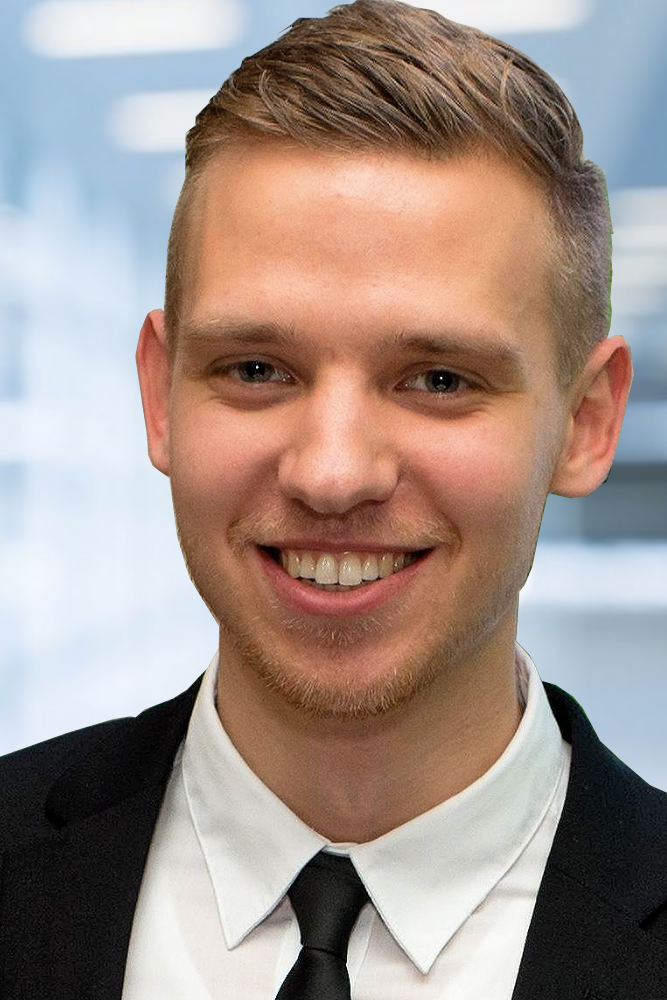
\includegraphics[height=3cm]{fig/lec01/Kirchgaessner.png}
			\caption*{Wilhelm Kirchg�ssner}
	\end{figure}
	
	\column[T]{0.23\textwidth}
	\begin{figure}
		\centering
			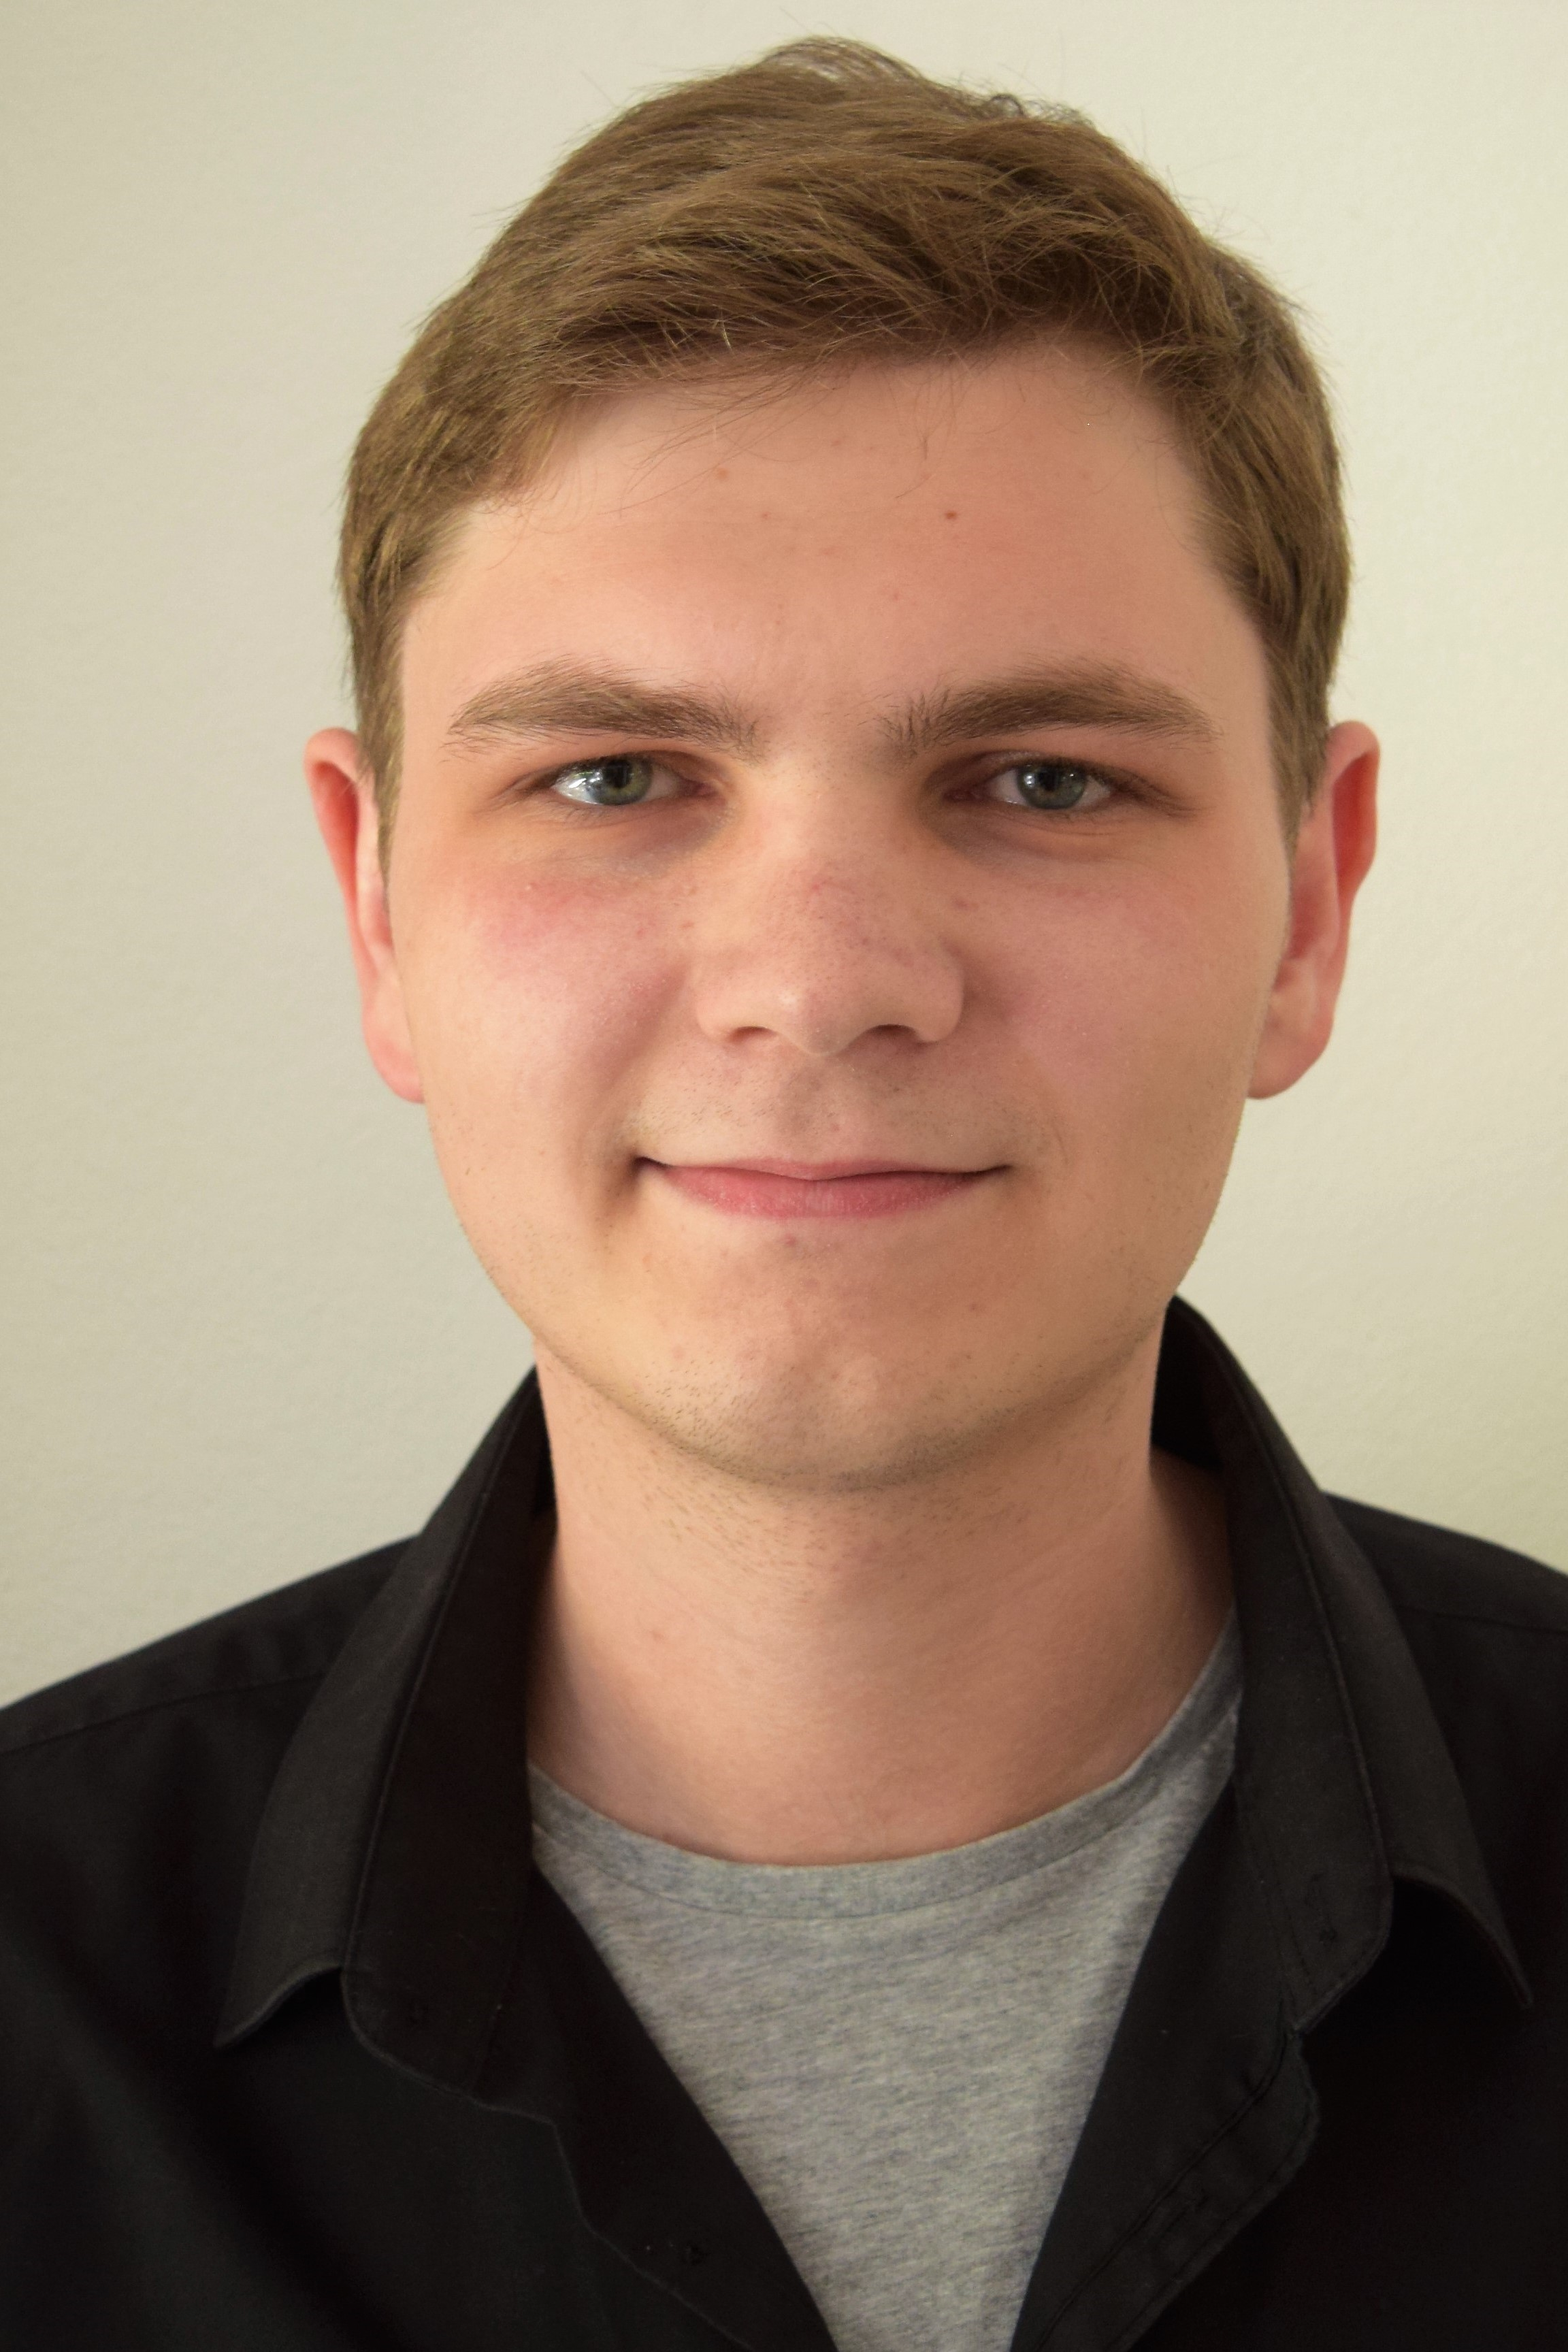
\includegraphics[height=3cm]{fig/lec01/Schenke.jpg}
			\caption*{Maximilian Schenke}
	\end{figure}
	
	\column[T]{0.23\textwidth}
	\begin{figure}
		\centering
			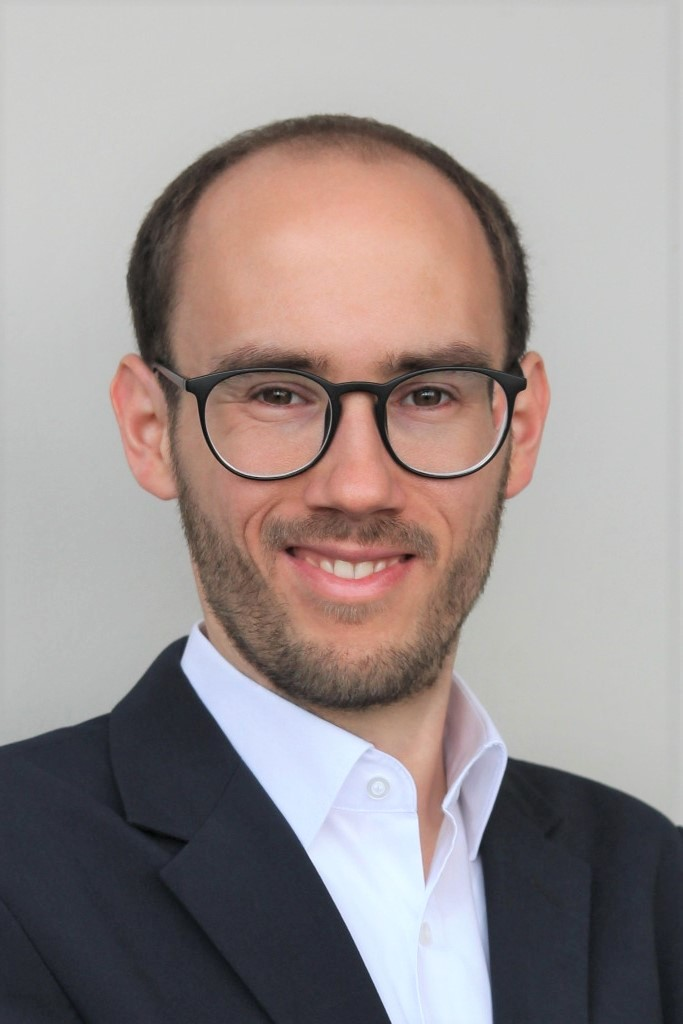
\includegraphics[height=3cm]{fig/lec01/Wallscheid.jpg}
			\caption*{Oliver\\ Wallscheid}
	\end{figure}
	
	\column[T]{0.23\textwidth}
	\begin{figure}
		\centering
			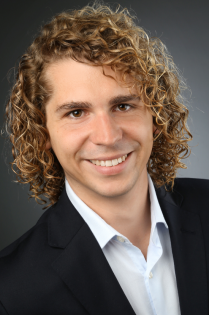
\includegraphics[height=3cm]{fig/lec01/Weber.png}
			\caption*{Daniel\\ Weber}
	\end{figure}
\end{columns}
\vspace{-0.25cm}
\begin{block}{Contact}
	\begin{itemize}
		\item Email: \href{mailto:wallscheid@lea.upb.de; weber@lea.upb.de; kirchgaessner@lea.upb.de; schenke@lea.upb.de}{\{kirchgaessner, schenke, wallscheid, weber\}$@$lea.upb.de}
		\item Offices: E-building, 4th floor
		\item Individual appointments on request (remote or personally)
	\end{itemize}
\end{block}
\end{frame}

%%%%%%%%%%%%%%%%%%%%%%%%%%%%%%%%%%%%%%%%%%%%%%%%%%%%%%%%%%%%%
%% Course Communication: Panda %%
%%%%%%%%%%%%%%%%%%%%%%%%%%%%%%%%%%%%%%%%%%%%%%%%%%%%%%%%%%%%%
\begin{frame}
\frametitle{Course Communication: Panda}
\begin{block}{Panda}
\begin{itemize}
		\item Paderborn Moodle clone (open-source learning management system)
		\item Please use it for any content-related or administrative communication
		\item Course materials / homework deliverables
	\end{itemize}
\end{block}

\begin{figure}
		\centering
			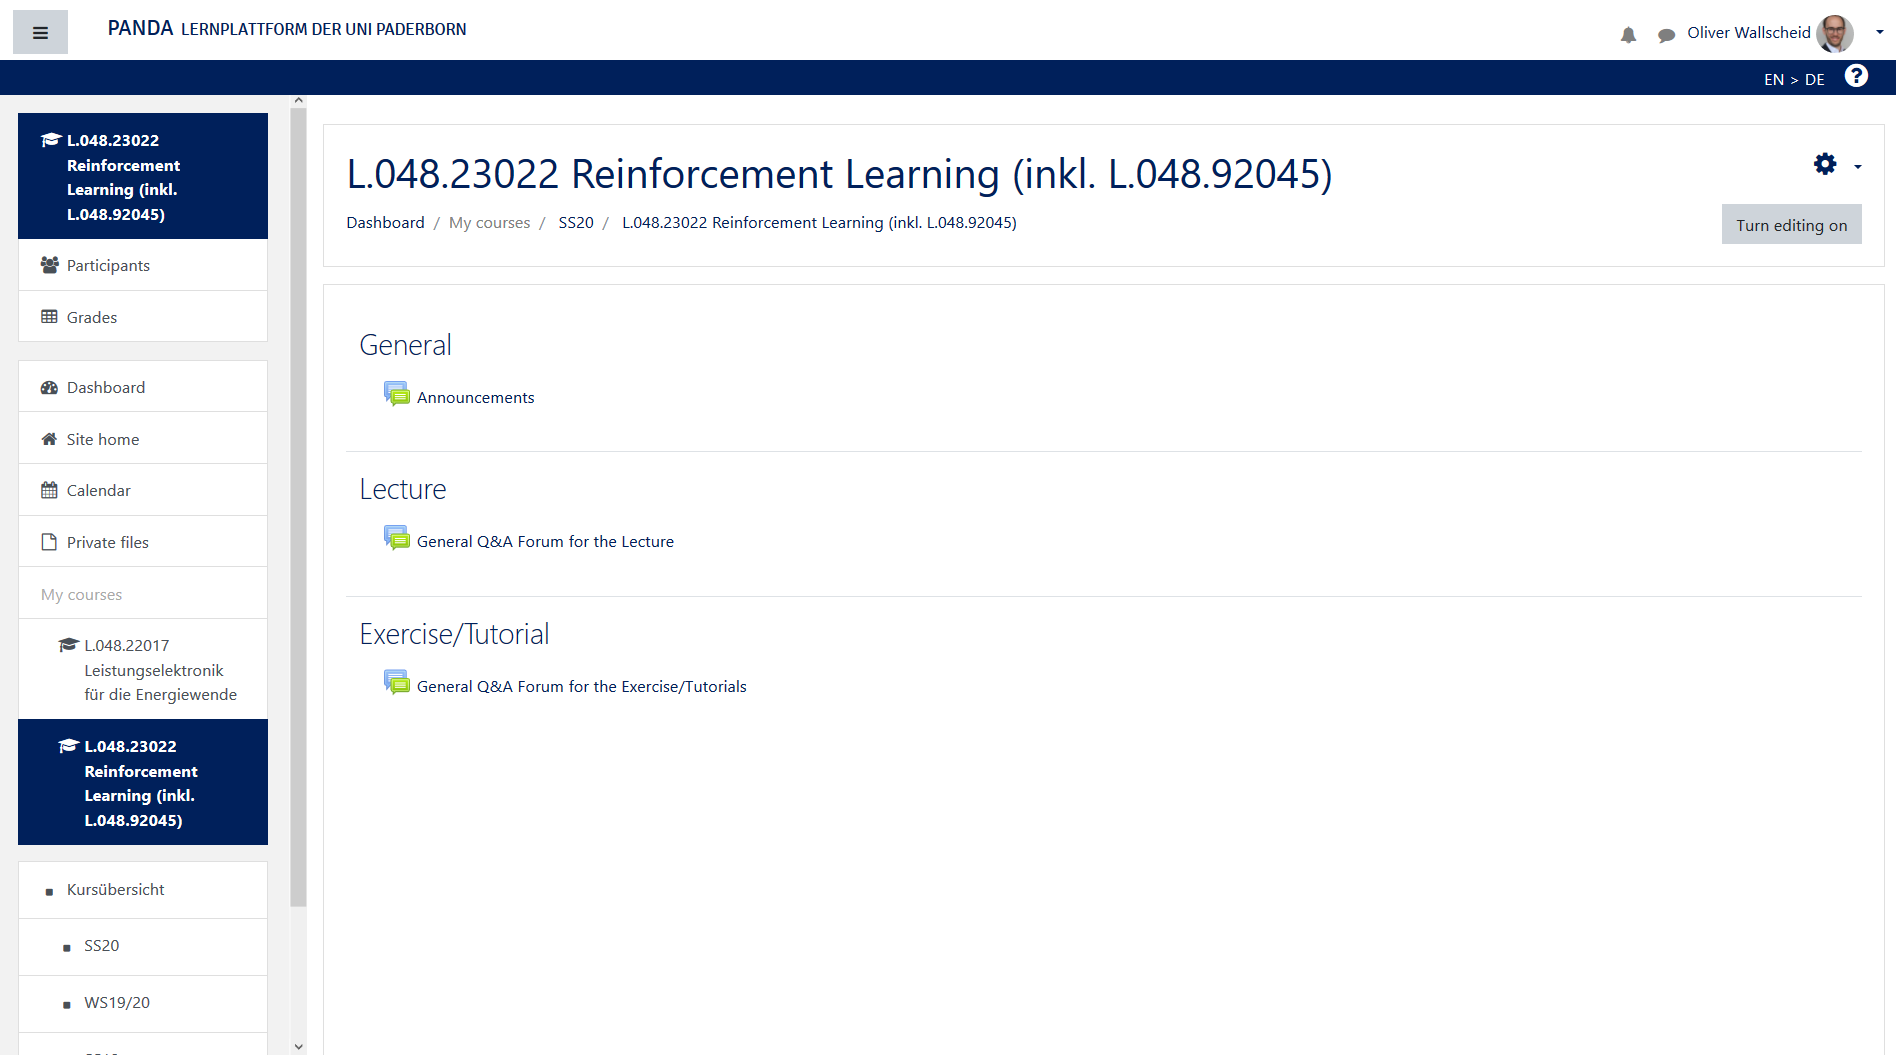
\includegraphics[height=4.8cm]{fig/lec01/Panda.png}
	\end{figure}
\end{frame}

%%%%%%%%%%%%%%%%%%%%%%%%%%%%%%%%%%%%%%%%%%%%%%%%%%%%%%%%%%%%%%
%%% Examination Regulations %%
%%%%%%%%%%%%%%%%%%%%%%%%%%%%%%%%%%%%%%%%%%%%%%%%%%%%%%%%%%%%%%
%\begin{frame}
%\frametitle{Examination Regulations}
%\begin{block}{Final exam}
%\begin{itemize}
	%\item Oral examination or written (waiting on executive board guidelines)
	%\item 30-45 minutes (oral) / 90-120 minutes (written)
	%\item Final decision in coming weeks
%\end{itemize}
%\end{block}
%\pause
%\begin{block}{Homework assignments}
%\begin{itemize}
	%\item 3x homework sheets with 1-2 week deadlines
	%\item Coding and classical question-answer queries
	%\item Equally distributed over lecture time frame
	%\item Homework sheet passed if  \unit{50+\,}{\%} points obtained
	%\item Regulation:
	%\begin{itemize}
		%\item Admission to final exam: min. 2 tests passed 
		%\item If all 3 tests passed: $1/3$ grade step
	%\end{itemize}
%\end{itemize}
%\end{block}
%\end{frame}


%%%%%%%%%%%%%%%%%%%%%%%%%%%%%%%%%%%%%%%%%%%%%%%%%%%%%%%%%%%%%
%% Course Outline %%
%%%%%%%%%%%%%%%%%%%%%%%%%%%%%%%%%%%%%%%%%%%%%%%%%%%%%%%%%%%%%
\begin{frame}
\frametitle{Course Outline}
The course will cover the following content (not necessarily in that order):
\vspace{0.25cm}
\begin{itemize}
		\item Conceptual basics and historical overview
		\item Markov decision processes
		\item Dynamic programming
		\item Monte Carlo learning
		\item Temporal difference learning
		\item Bootstrapping
		\item On- and Off-policy strategies
		\pause
		\item Function approximation and deep learning
		\item Policy gradient methods
		\pause
		\item Safe reinforcement learning
		\item Integration of expert (pre-)knowledge
	\end{itemize}
\end{frame}

%%%%%%%%%%%%%%%%%%%%%%%%%%%%%%%%%%%%%%%%%%%%%%%%%%%%%%%%%%%%%
%% Textbooks %%
%%%%%%%%%%%%%%%%%%%%%%%%%%%%%%%%%%%%%%%%%%%%%%%%%%%%%%%%%%%%%
\begin{frame}
\frametitle{Recommended Textbooks}
\begin{itemize}
		\item Reinforcement learning: an introduction, 
		\begin{itemize}
			\item R. Sutton and G. Barto
			\item MIT Press, 2nd edition, 2018
			\item Available in library plus electronic copy in Panda
		\end{itemize}
		\vspace{0.5cm}
		\pause
		\item Reinforcement learning (lecture script)
		\begin{itemize}
		  \item D. Silver
			\item Entire slide set on Panda and available \href{https://www.davidsilver.uk/teaching/}{here}
			\item YouTube lecture series (click \href{https://www.youtube.com/watch?v=2pWv7GOvuf0}{here})
		\end{itemize}
		\vspace{0.5cm}
		\pause
		\item Reinforcement learning and optimal control
		\begin{itemize}
			\item D. Bertsekas
			\item Athena Scientific, 2019
			\item Available in library
		\end{itemize}
		
	\end{itemize}
\end{frame}


%%%%%%%%%%%%%%%%%%%%%%%%%%%%%%%%%%%%%%%%%%%%%%%%%%%%%%%%%%%%%
\section{Reinforcement Learning: What is it?} 
%%%%%%%%%%%%%%%%%%%%%%%%%%%%%%%%%%%%%%%%%%%%%%%%%%%%%%%%%%%%%

\begin{frame}
\frametitle{Table of Contents}
\tableofcontents[currentsection]
\end{frame}

%%%%%%%%%%%%%%%%%%%%%%%%%%%%%%%%%%%%%%%%%%%%%%%%%%%%%%%%%%%%%
%% RL Wiki Optimization Cricle %%
%%%%%%%%%%%%%%%%%%%%%%%%%%%%%%%%%%%%%%%%%%%%%%%%%%%%%%%%%%%%%
\frame{\frametitle{The Basic Reinforcement Learning Structure}
\begin{columns}[t,onlytextwidth]
\begin{column}{0.6\textwidth}
\begin{minipage}[c]{\linewidth}
	\begin{figure}
		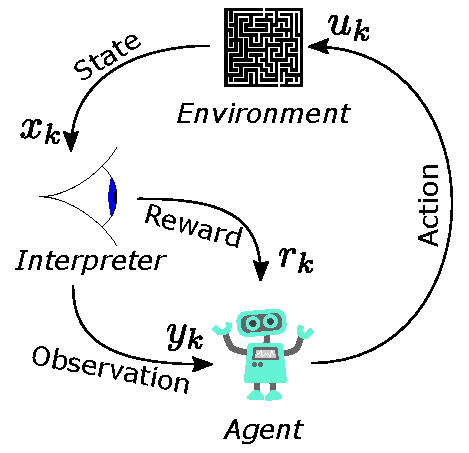
\includegraphics[width=5.99cm]{fig/lec01/RL_Wiki.pdf}
		\caption{The basic RL operation principle\\(derivative of \href{https://commons.wikimedia.org/wiki/File:Reinforcement_learning_diagram.svg}{www.wikipedia.org}, \href{https://creativecommons.org/publicdomain/zero/1.0/deed.en}{CC0 1.0})}
		\label{fig:RL_Wiki}
	\end{figure}
\end{minipage}
\end{column}
\hfill
\begin{column}{0.38\textwidth}
\begin{minipage}[c]{\linewidth}
\vspace{0.3cm}
Key characteristics:
	\begin{itemize}
		\item No supervisor
		\item Data-driven
		\item Discrete time steps
		\item Sequential data stream (not i.i.d. data)
		\item Agent actions affect subsequent data (sequential decision making)
	\end{itemize}
\end{minipage}
\end{column}
\end{columns}
\blfootnote{The nomenclature of this script is based on the default variable usage in control theory. In other RL books, one often finds $s$ as state, $a$ as action and $o$ as observation.}
}

%%%%%%%%%%%%%%%%%%%%%%%%%%%%%%%%%%%%%%%%%%%%%%%%%%%%%%%%%%%%%
%% Agent and Environment %%
%%%%%%%%%%%%%%%%%%%%%%%%%%%%%%%%%%%%%%%%%%%%%%%%%%%%%%%%%%%%%
\frame{\frametitle{Agent and Environment}
\begin{minipage}[t]{0.5\linewidth}
	\begin{figure}
		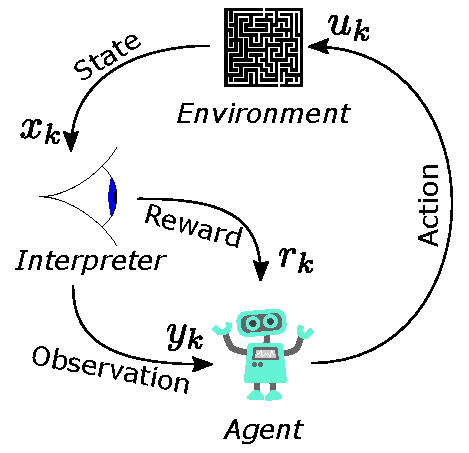
\includegraphics[width=5cm]{fig/lec01/RL_Wiki.pdf}
	\end{figure}
\end{minipage}
\hfill
\begin{minipage}[t]{0.48\linewidth}

At each step $k$ the agent:
	\begin{itemize}
		\item Picks an action $u_k$.
		\item Receives an observation $y_k$.
		\item Receives a reward $r_k$.
	\end{itemize}
\pause
At each step $k$ the environment:
	\begin{itemize}
		\item Receives an action $u_k$.
		\item Emits an observation $y_{k+1}$.
		\item Emits a reward $r_{k+1}$.
	\end{itemize}
The time increments $k \leftarrow k+1$.	
\end{minipage}
\pause
\begin{block}{Remark on time}
Classically, a one step time delay is assumed between executing the action and receiving the corresponding observation and reward. In many applications the resulting time interval $\Delta T = t_k - t_{k+1}$ is a constant.
\end{block}
}

%%%%%%%%%%%%%%%%%%%%%%%%%%%%%%%%%%%%%%%%%%%%%%%%%%%%%%%%%%%%%
%% What is Learning? %%
%%%%%%%%%%%%%%%%%%%%%%%%%%%%%%%%%%%%%%%%%%%%%%%%%%%%%%%%%%%%%
\frame{\frametitle{Some Basic Definitions from the Literature}
What is reinforcement?
\begin{itemize}
	\item ``\textit{Reinforcement is a consequence applied that will strengthen an organism's future behavior whenever that behavior is preceded by a specific antecedent stimulus.[...]There are two types of reinforcement, known as positive reinforcement and negative reinforcement; positive is where by a reward is offered on expression of the wanted behaviour and negative is taking away an undesirable element in the persons environment whenever the desired behaviour is achieved.}'', \href{https://en.wikipedia.org/wiki/Reinforcement}{wikipedia.org} (obtained 2020-02-07) 
\end{itemize}
\pause
\vspace{0.3cm}
What is learning?
\begin{itemize}
	\item ``\textit{Acquiring knowledge and skills and having them readily available from memory so you can make sense of future problems and opportunities.}'', From Make It Stick: The Science of Successful Learning, Brown et al., Harvard Press, 2014
\end{itemize}
}

%%%%%%%%%%%%%%%%%%%%%%%%%%%%%%%%%%%%%%%%%%%%%%%%%%%%%%%%%%%%%
%% RL vs. (un-)supervised learning %%
%%%%%%%%%%%%%%%%%%%%%%%%%%%%%%%%%%%%%%%%%%%%%%%%%%%%%%%%%%%%%
\frame{\frametitle{Context Around Reinforcement Learning}
\begin{figure}
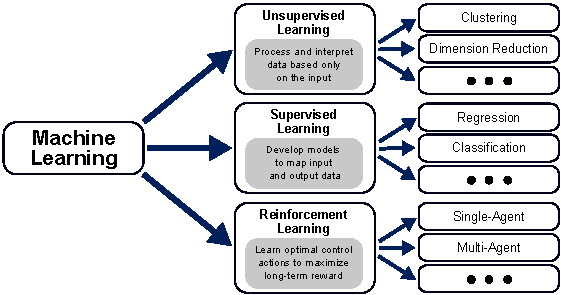
\includegraphics[width=11cm]{fig/lec01/Machine_Learning_Disciplines.pdf}
\caption{Disciplines of machine learning}
\label{fig:Machine_Learning_Disciplines}
\end{figure}
}

%%%%%%%%%%%%%%%%%%%%%%%%%%%%%%%%%%%%%%%%%%%%%%%%%%%%%%%%%%%%%
%% Context Around Machine Learning %%
%%%%%%%%%%%%%%%%%%%%%%%%%%%%%%%%%%%%%%%%%%%%%%%%%%%%%%%%%%%%%
\frame{\frametitle{Context Around Machine Learning}
\begin{figure}
\centering
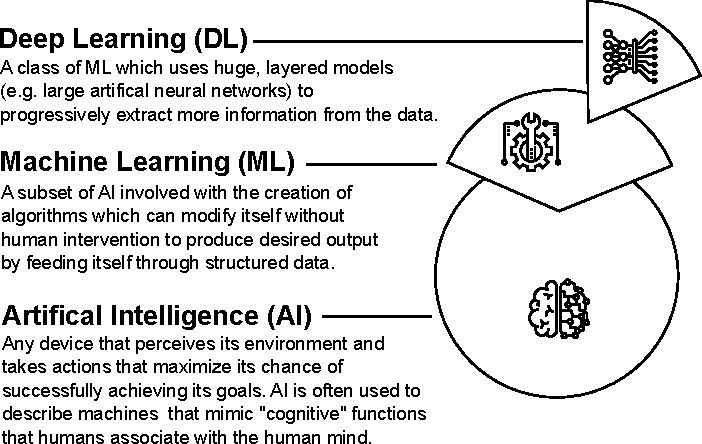
\includegraphics[width=11cm]{fig/lec01/ML_AI.pdf}
\caption{The broader scope around machine learning}
\label{fig:ML_AI}
\end{figure}
}

%%%%%%%%%%%%%%%%%%%%%%%%%%%%%%%%%%%%%%%%%%%%%%%%%%%%%%%%%%%%%
%% Many Faces of Reinforcement Learning (D.Silver) %%
%%%%%%%%%%%%%%%%%%%%%%%%%%%%%%%%%%%%%%%%%%%%%%%%%%%%%%%%%%%%%
\frame{\frametitle{Many Faces of Reinforcement Learning}
\begin{figure}
\centering
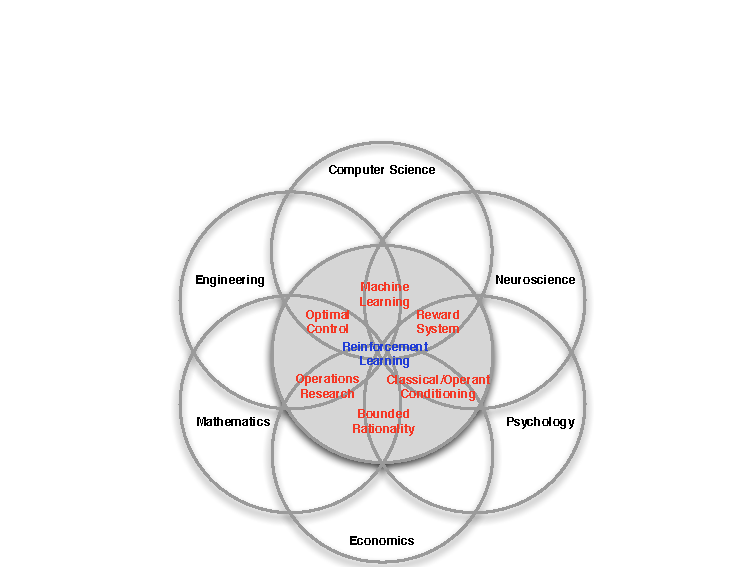
\includegraphics[width=6cm]{fig/lec01/Faces_RL.pdf}
\caption{RL and its neighboring domains\\ \SilverLectureSource}
\label{fig:Faces_RL}
\end{figure}
}

%%%%%%%%%%%%%%%%%%%%%%%%%%%%%%%%%%%%%%%%%%%%%%%%%%%%%%%%%%%%%%%%%%
\section{Application Examples and Historic Review} 
%%%%%%%%%%%%%%%%%%%%%%%%%%%%%%%%%%%%%%%%%%%%%%%%%%%%%%%%%%%%%%%%%%
\begin{frame}
\frametitle{Table of Contents}
\tableofcontents[currentsection]
\end{frame}

%%%%%%%%%%%%%%%%%%%%%%%%%%%%%%%%%%%%%%%%%%%%%%%%%%%%%%%%%%%%%
%% Methodical origins %%
%%%%%%%%%%%%%%%%%%%%%%%%%%%%%%%%%%%%%%%%%%%%%%%%%%%%%%%%%%%%%
\frame{\frametitle{Methodical Origins}
\begin{minipage}[t]{0.32\linewidth}
	\begin{figure}
		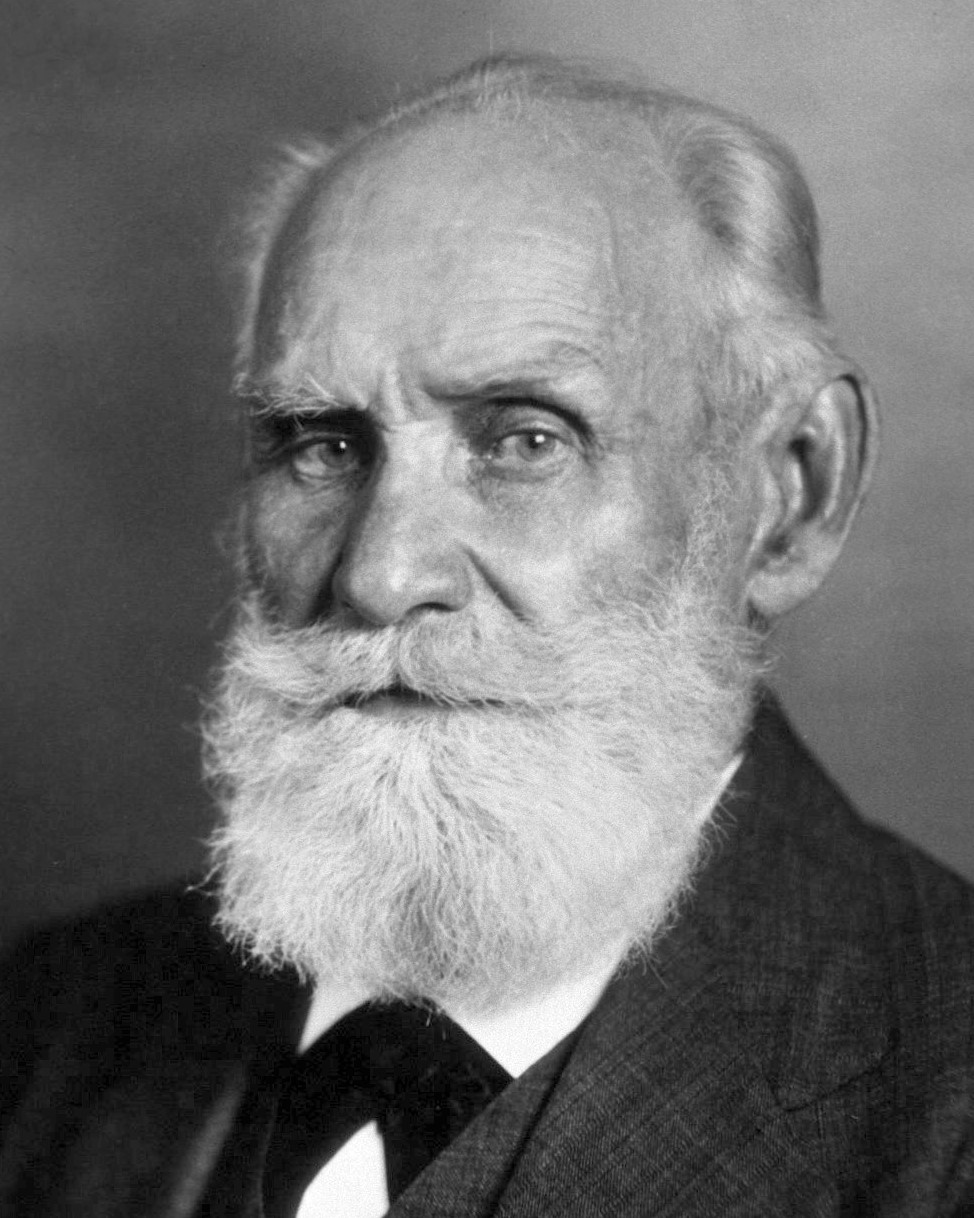
\includegraphics[width=3.0cm]{fig/lec01/Pavlov.jpg}
		\caption{Ivan Pavlov\\(1849-1936)}
	\end{figure}
	\begin{itemize}
		\item Classical conditioning
	\end{itemize}
\end{minipage}
\hfill
\begin{minipage}[t]{0.32\linewidth}
	\begin{figure}
		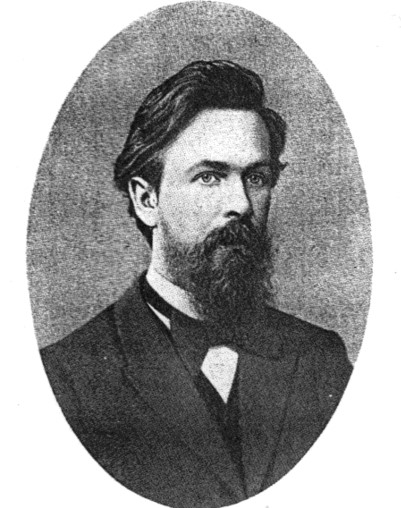
\includegraphics[width=3.0cm]{fig/lec01/Markov.jpg}
		\caption{Andrei Markov\\(1856-1922)}
	\end{figure}
	\begin{itemize}
		\item Stochastic process formalism 
	\end{itemize}
\end{minipage}
\hfill
\begin{minipage}[t]{0.32\linewidth}
	\begin{figure}
		
\includegraphics[width=3.0cm]{fig/lec01/Bell_man.pdf}
		\caption{Richard Bellman\\(1920-1984)\footnotemark}
	\end{figure}
	\begin{itemize}
		\item Optimal sequential decision making
	\end{itemize}
\end{minipage}
\footnotetext{Illustrative picture since an actual photo of Bellman is not freely available.}
}

%%%%%%%%%%%%%%%%%%%%%%%%%%%%%%%%%%%%%%%%%%%%%%%%%%%%%%%%%%%%%
%% RL History %%
%%%%%%%%%%%%%%%%%%%%%%%%%%%%%%%%%%%%%%%%%%%%%%%%%%%%%%%%%%%%%
\frame{\frametitle{History of Reinforcement Learning}
Huge field with many interconnections to different fields. One could give a lecture only on the historic development. Hence, interested readers are referred to:
\begin{itemize}
	\item Chapter 1.7 of Barto/Sutton, \textit{Reinforcement learning: an introduction}, 2nd edition, MIT Press, 2018 
	\item 30 minutes talk of A. Barto \href{https://www.youtube.com/watch?v=ul6B2oFPNDM}{(YouTube link)}
	\item Paper on more recent developments: Arulkumaran et al., \textit{A Brief Survey of Deep Reinforcement Learning}, \href{https://arxiv.org/abs/1708.05866}{arXiv:1708.05866}, 2017  
\end{itemize}
}


%%%%%%%%%%%%%%%%%%%%%%%%%%%%%%%%%%%%%%%%%%%%%%%%%%%%%%%%%%%%%
%% Application Examples %%
%%%%%%%%%%%%%%%%%%%%%%%%%%%%%%%%%%%%%%%%%%%%%%%%%%%%%%%%%%%%%
\frame{\frametitle{Contemporary Application Examples}
Limited selection from a broad field:
\begin{itemize}
	\item \href{https://www.youtube.com/watch?v=Lt-KLtkDlh8}{Swinging-up and balance a cart-pole / an inverted pendulum}
	\item \href{https://www.youtube.com/watch?v=W_gxLKSsSIE}{Flipping pancakes with a roboter arm}
	\item \href{https://arxiv.org/abs/1910.09434}{Controlling electric drive systems}
	\item \href{https://www.youtube.com/watch?v=opsmd5yuBF0}{Drifting with a RC-car}
	\item \href{https://www.youtube.com/watch?v=eRwTbRtnT1I}{Driving an autonomous car}
	\item \href{https://www.youtube.com/watch?v=eG1Ed8PTJ18}{Playing Atari Breakout}
	\item \href{https://www.youtube.com/watch?v=9xlSy9F5WtE}{Play strategy board game Go at super-human performance}
	\item \href{https://arxiv.org/abs/1811.07522}{Making money with stock trading}
	\item ...
\end{itemize}
}


%%%%%%%%%%%%%%%%%%%%%%%%%%%%%%%%%%%%%%%%%%%%%%%%%%%%%%%%%%%%%%%%%%
\section{Basic Terminology} 
%%%%%%%%%%%%%%%%%%%%%%%%%%%%%%%%%%%%%%%%%%%%%%%%%%%%%%%%%%%%%%%%%%
\begin{frame}
\frametitle{Table of Contents}
\tableofcontents[currentsection]
\end{frame}

%%%%%%%%%%%%%%%%%%%%%%%%%%%%%%%%%%%%%%%%%%%%%%%%%%%%%%%%%%%%%
%% Reward basics %%
%%%%%%%%%%%%%%%%%%%%%%%%%%%%%%%%%%%%%%%%%%%%%%%%%%%%%%%%%%%%%
\frame{\frametitle{Vocabulary Preview}
In this section, some of the most important RL terms are shortly explained and summarized:
\begin{itemize}
	\item Reward and return
	\item State
	\item Action
	\item Policy
	\item Value function
	\item Model
	\item Exploration and exploitation
\end{itemize}
}

%%%%%%%%%%%%%%%%%%%%%%%%%%%%%%%%%%%%%%%%%%%%%%%%%%%%%%%%%%%%%
%% Reward basics %%
%%%%%%%%%%%%%%%%%%%%%%%%%%%%%%%%%%%%%%%%%%%%%%%%%%%%%%%%%%%%%
\frame{\frametitle{Reward}
\begin{itemize}
	\item A \hl{reward} is a scalar \hl{random variable} $R_k$ with \hl{realizations} $r_k$.
	\item Often it is considered a real-number $r_k\in\mathbb{R}$ or an integer $r_k\in\mathbb{Z}$.\pause
	\item The reward function (interpreter) may be naturally given or is a design degree of freedom (i.e., can be manipulated).\pause 
	\item It fully indicates how well an RL agent is doing at step $k$.
	\item Hence, the agent's task is to maximize its reward over time.\pause
\end{itemize}
\begin{theo}{Reward hypothesis}{reward_hypo}
All goals can be described by the maximization of the expected cumulative reward:
\begin{equation}
	\max \E{\sum_{i=0}^\infty R_{k+i+1}} .
\end{equation}
\end{theo} 
\pause
Question: Which situations may conflict with the reward hypothesis?
}


%%%%%%%%%%%%%%%%%%%%%%%%%%%%%%%%%%%%%%%%%%%%%%%%%%%%%%%%%%%%%
%% Reward examples %%
%%%%%%%%%%%%%%%%%%%%%%%%%%%%%%%%%%%%%%%%%%%%%%%%%%%%%%%%%%%%%
\frame{\frametitle{Reward Examples}
\begin{itemize}
	\item Flipping a pancake:
	\begin{itemize}
		\item Pos. reward: catching the $\unit{180}{^\circ}$ rotated pancake 
		\item Neg. reward: droping the pancake on the floor
	\end{itemize}
	\pause
	\item Stock trading:
	\begin{itemize}
		\item Trading portfolio monetary value 
	\end{itemize}
	\pause
	\item Playing Atari games:
	\begin{itemize}
		\item Highscore value at the end of a game episode
	\end{itemize}
	\pause
	\item Driving an autonomous car:
	\begin{itemize}
		\item Pos. reward: getting save from A to B without crashing
		\item Neg. reward: hitting another car,  pedestrian, bicycle,...
	\end{itemize}
	\pause
	\item Classical control task (e.g inverted pendulum, electric drive):
	\begin{itemize}
		\item Pos. reward: following a given reference trajectory precisely
		\item Neg. reward: violating system constraints and/or large control error
	\end{itemize}
\end{itemize}
}

%%%%%%%%%%%%%%%%%%%%%%%%%%%%%%%%%%%%%%%%%%%%%%%%%%%%%%%%%%%%%
%% Reward characteristics %%
%%%%%%%%%%%%%%%%%%%%%%%%%%%%%%%%%%%%%%%%%%%%%%%%%%%%%%%%%%%%%
\frame{\frametitle{Reward Characteristics}
Rewards can have many different flavors and are highly depending on the given problem:
\begin{itemize}
	\item Actions may have short and/or long term consequences.
	\begin{itemize}
		\item The reward for a certain action may be delayed.
		\item Examples: Stock trading, strategic board games,...
	\end{itemize}
	\pause
	\item Rewards can be positive and negative real values.
	\begin{itemize}
		\item Certain situations (e.g. car hits wall) might lead to a negative reward.
	\end{itemize}
	\pause
	\item Exogenous impacts might introduce stochastic reward components.
\begin{itemize}
	\item Example: A wind gust pushes the helicopter into a tree. 
\end{itemize}
\end{itemize}
\pause
\begin{block}{Remark on reward}
The RL agent's learning process is heavily linked with the reward distribution over time. Designing expedient rewards functions is therefore crucially important for successfully applying RL. And often there is no predefined way on how to design the ``best reward function''.
\end{block}
}

%%%%%%%%%%%%%%%%%%%%%%%%%%%%%%%%%%%%%%%%%%%%%%%%%%%%%%%%%%%%%
%% King Midas %%
%%%%%%%%%%%%%%%%%%%%%%%%%%%%%%%%%%%%%%%%%%%%%%%%%%%%%%%%%%%%%
\frame{\frametitle{The Reward Function Hassle}
\begin{itemize}
	\item ``Be careful what you wish for - you might get it'' (pro-verb)
	\item ``...it grants what you ask for, not what you should have asked for or what you intend.'' (Norbert Wiener, American mathematician)
\end{itemize}
\begin{figure}
		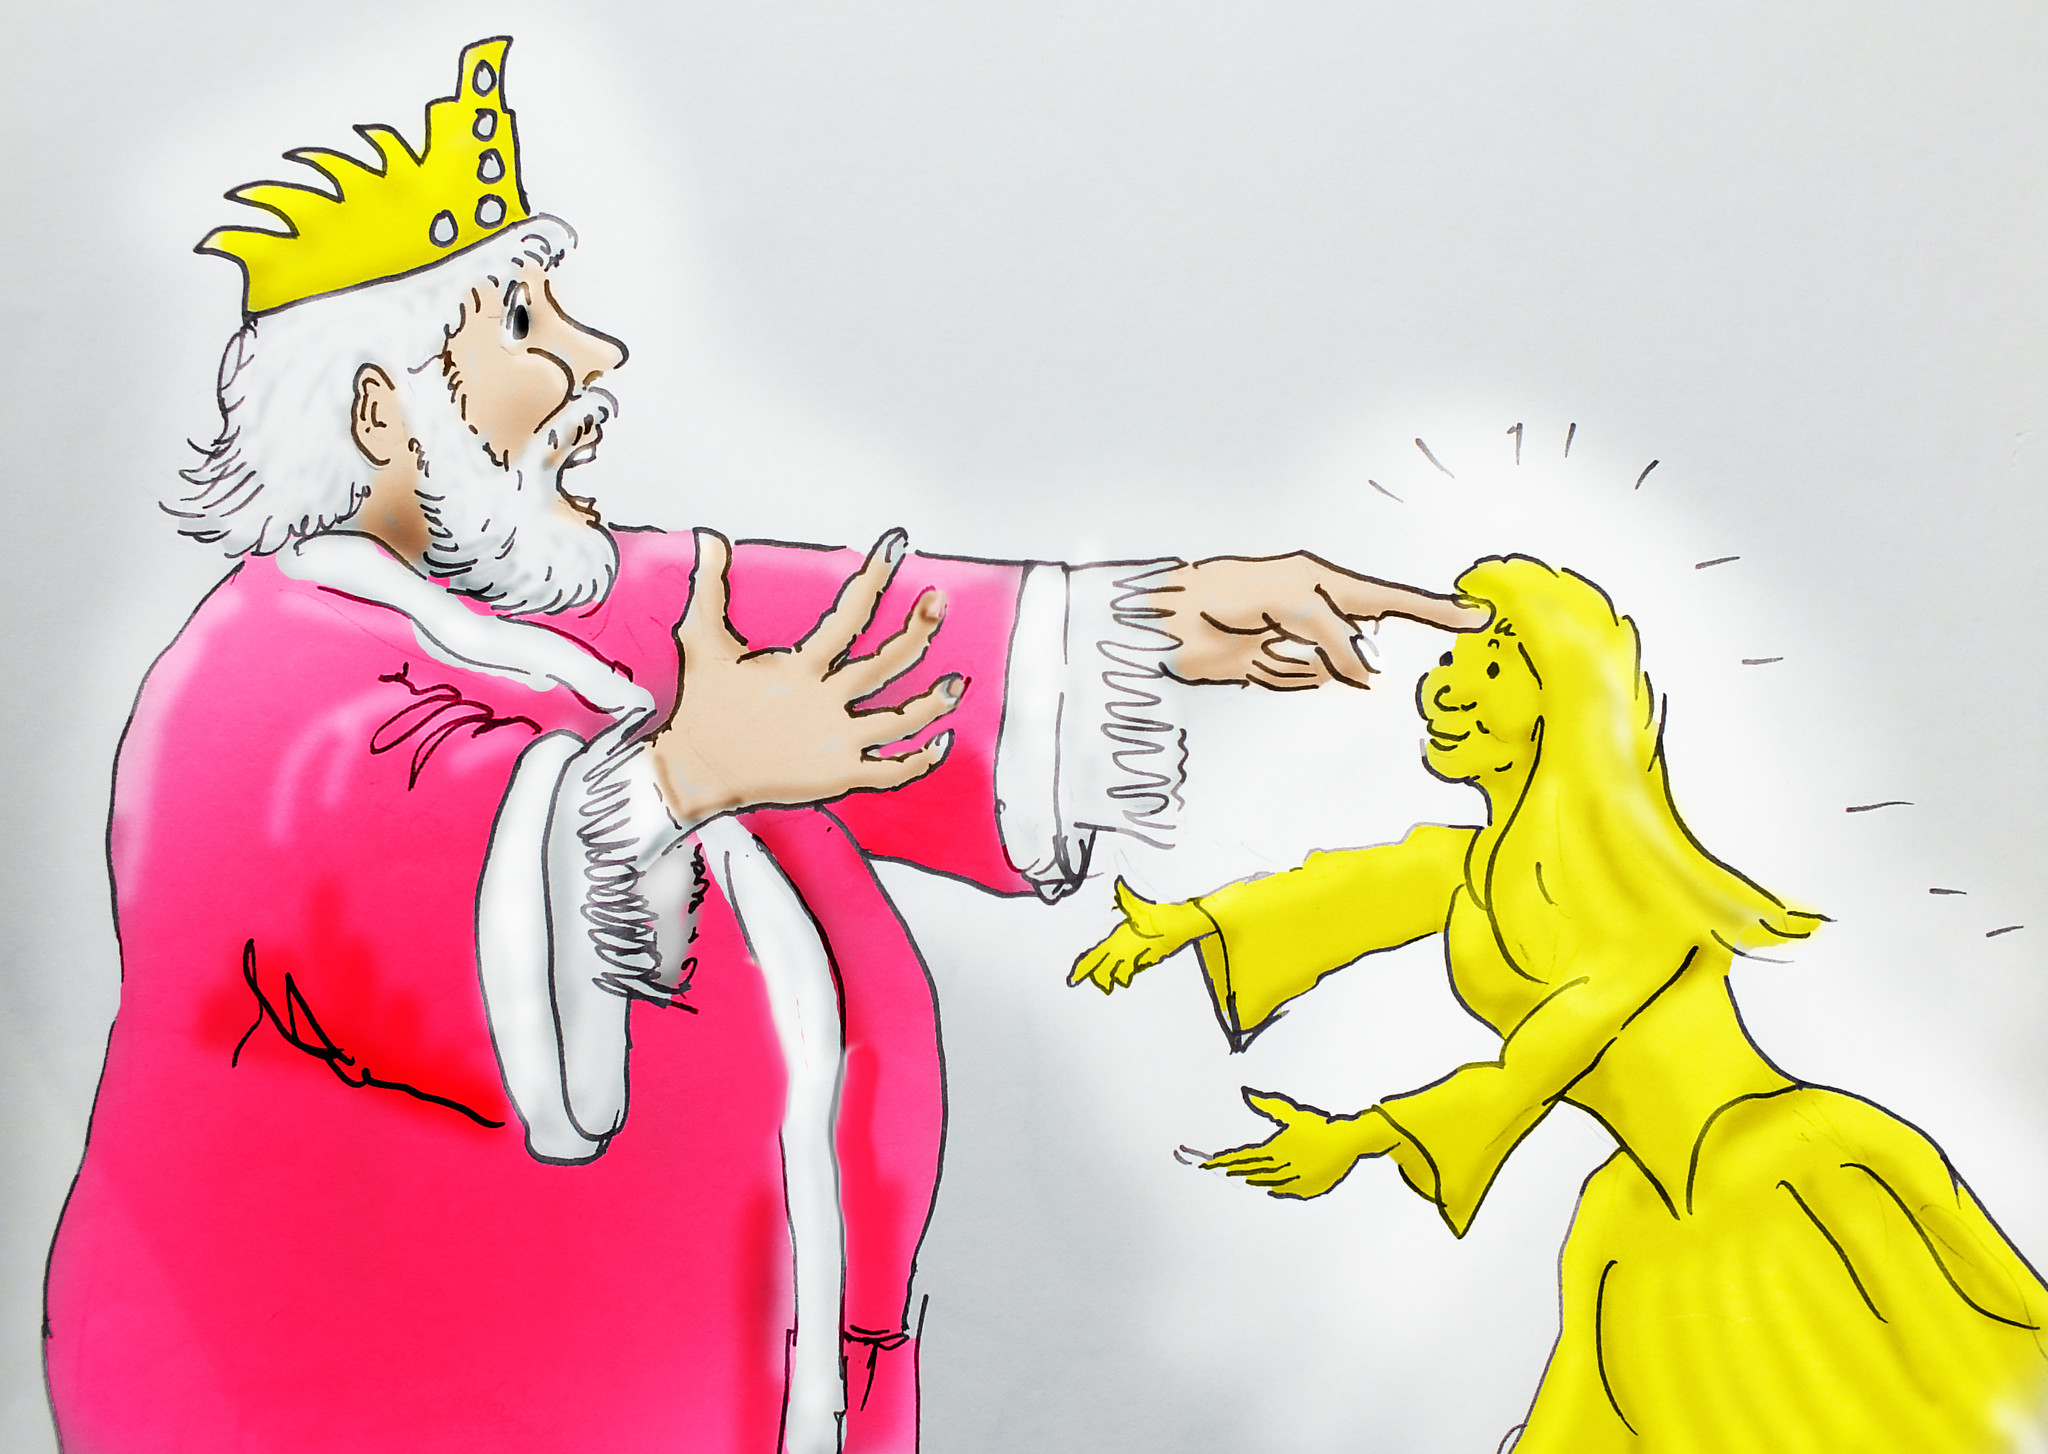
\includegraphics[width=6cm]{fig/lec01/Midas.jpg}
		\caption{Midas and Daughter (Good as Gold)\\(source: \href{https://www.flickr.com/photos/robinhutton/16403846414/in/photostream/}{www.flickr.com}, by \href{https://www.flickr.com/photos/robinhutton/}{Robin Hutton} \href{https://creativecommons.org/licenses/by-nc-nd/2.0/}{CC BY-NC-ND 2.0})}
		\label{fig:Midas}
	\end{figure}
}

%%%%%%%%%%%%%%%%%%%%%%%%%%%%%%%%%%%%%%%%%%%%%%%%%%%%%%%%%%%%%
%% Task-dependent return definitions %%
%%%%%%%%%%%%%%%%%%%%%%%%%%%%%%%%%%%%%%%%%%%%%%%%%%%%%%%%%%%%%
\frame{\frametitle{Task-Dependent Return Definitions}
\hlh{Episodic tasks}
\begin{itemize}
	\item A problem which naturally breaks into subsequences (\hl{episodes}).
	\item Examples: Most games, maze,...
	\item The \hl{return} becomes a finite sum:
	\begin{equation}
	g_k = r_{k+1} + r_{k+2} + \cdots + r_{N}\, .	
	\end{equation}
	\item Episodes end at their terminal step $k=N$.
\end{itemize}
\pause
\hlh{Continuing tasks}
\begin{itemize}
	\item A problem which lacks a natural end (\hl{infinite horizon}).
	\item Example: Process control tasks
	\item The return should be \hl{discounted} to prevent infinite numbers:
	\begin{equation}
	\label{eq:return_disc}
	g_k = r_{k+1} + \gamma r_{k+2} + \gamma^2 r_{k+3} + \cdots = \sum_{i=0}^\infty \gamma^i r_{k+i+1}\, .  	
	\end{equation}
	\item Here, $\gamma\in\left\{\mathbb{R}|0 \leq \gamma \leq 1\right\}$ is the \hl{discount rate}.
\end{itemize}
}

%%%%%%%%%%%%%%%%%%%%%%%%%%%%%%%%%%%%%%%%%%%%%%%%%%%%%%%%%%%%%
%% Disounted rewards %%
%%%%%%%%%%%%%%%%%%%%%%%%%%%%%%%%%%%%%%%%%%%%%%%%%%%%%%%%%%%%%
\frame{\frametitle{Discounted Rewards}
\hlh{Numeric viewpoint}
\begin{itemize}
	\item If $\gamma =1$ and $r_k >> 0$ for $k\rightarrow\infty$, $g_k$ in \eqref{eq:return_disc} gets infinite.
	\item If $\gamma <1$ and $r_k$ is bounded for $k\rightarrow\infty$, $g_k$ in \eqref{eq:return_disc} is bounded.
\end{itemize}
\pause
\hlh{Strategic viewpoint}
\begin{itemize}
	\item If $\gamma \approx 1$: agent is farsighted.
	\item If $\gamma \approx 0$: agent is shortsighted (only interested in immediate reward).
\end{itemize}
\pause
\hlh{Mathematical options}
\begin{itemize}
	\item The current return is the discounted future return:
\begin{equation}
	\begin{split}
		g_k &= r_{k+1} + \gamma r_{k+2} + \gamma^2 r_{k+3} + \cdots\\
				&= r_{k+1} + \gamma \left(r_{k+2} + \gamma r_{k+3} + \cdots \right)\\
				&= r_{k+1} + \gamma g_{k+1}\, .
	\end{split}
\end{equation}
\pause
	\item If $r_k=r$ is a constant and $\gamma<1$ one receives:
	\begin{equation}
		g_k = \sum_{i=0}^\infty \gamma^i r = r \sum_{i=0}^\infty \gamma^i = r\frac{1}{1-\gamma}\, .
	\end{equation}
\end{itemize}
}

%%%%%%%%%%%%%%%%%%%%%%%%%%%%%%%%%%%%%%%%%%%%%%%%%%%%%%%%%%%%%
%% The env. state %%
%%%%%%%%%%%%%%%%%%%%%%%%%%%%%%%%%%%%%%%%%%%%%%%%%%%%%%%%%%%%%
\frame{\frametitle{State (1)}
\hlh{Environment state}  \blfootnote{\hl{Bold symbols} are non-scalar multidimensional quantities e.g. vectors and matrices.}
\begin{itemize}
	\item Random variable $\bm{X}_k^e$ with realizations $\bm{x}_k^e$ \blfootnote{\hl{Capital symbols} denote random variables and small symbols their realizations.}
	\item Internal status representation of the environment, e.g
	\begin{itemize}
		\item Physical states e.g. car velocity or motor current
		\item Game states e.g. current chess board situation
		\item Financial states e.g. stock market status 
	\end{itemize}
	\pause
	\item  Fully, limited or not at all visible by the agent
	\begin{itemize}
		\item Sometimes even 'foggy' or uncertain
		\item In general: $\bm{Y}_k = \bm{f}(\bm{X}_k)$
	\end{itemize}
	\pause
	\item Continuous or discrete quantity
\end{itemize}
}

%%%%%%%%%%%%%%%%%%%%%%%%%%%%%%%%%%%%%%%%%%%%%%%%%%%%%%%%%%%%%
%% The act. state %%
%%%%%%%%%%%%%%%%%%%%%%%%%%%%%%%%%%%%%%%%%%%%%%%%%%%%%%%%%%%%%
\frame{\frametitle{State (2)}
\hlh{Agent state} 
\begin{itemize}
  \item Random variable $\bm{X}_k^a$ with realizations $\bm{x}_k^a$ 
	\item Internal status representation of the agent
	\pause
	\item In general: $\bm{x}_k^a\neq \bm{x}_k^e$ (e.g. due to measurement noise)
	\pause
	\item Agent's condensed information relevant for next action
	\item Dependent on internal knowledge / policy representation of the agent
	\pause
	\item Continuous or discrete quantity
\end{itemize}
}

%%%%%%%%%%%%%%%%%%%%%%%%%%%%%%%%%%%%%%%%%%%%%%%%%%%%%%%%%%%%%
%% History and Imformation State%%
%%%%%%%%%%%%%%%%%%%%%%%%%%%%%%%%%%%%%%%%%%%%%%%%%%%%%%%%%%%%%
\frame{\frametitle{History and Information State}
\begin{defi}{History}{History}
The history is the past sequence of all observations, actions and rewards
\begin{equation}
	\mathbb{H}_k = \left\{\bm{y}_0, r_0, \bm{u}_0, \ldots, \bm{u}_{k-1}, \bm{y}_k, r_k\right\}
\end{equation}
up to the time step $k$.
\end{defi}
\pause
If the current state $\bm{x}_k$ contains all useful information from the history it is called an \hl{information or Markov state}:
\begin{defi}{Information state}{InfSate}
A state $\bm{X}_k$ is called an information state if and only if
\begin{equation}
	\Pb{\bm{X}_{k+1}|\bm{X}_k}=\Pb{\bm{X}_{k+1}|\bm{X}_0, \bm{X}_1,\ldots, \bm{X}_k}\, .
\end{equation}
\end{defi}
\pause
\begin{itemize}
	\item History is fully condensed in $\bm{x}_k$, i.e., $\bm{x}_{k+1}$ is only depending on $\bm{x}_k$.
	\item A given system can be fully described by $\bm{x}_k$.
\end{itemize}
}

%%%%%%%%%%%%%%%%%%%%%%%%%%%%%%%%%%%%%%%%%%%%%%%%%%%%%%%%%%%%%
%% State Example%%
%%%%%%%%%%%%%%%%%%%%%%%%%%%%%%%%%%%%%%%%%%%%%%%%%%%%%%%%%%%%%
\frame{\frametitle{Model Examples With Markov States}
Linear time-invariant (LTI) state space model
\begin{equation}
\begin{split}
	\bm{x}_{k+1} &= \bm{A}\bm{x}_k +\bm{B}\bm{u}_k\, ,\\
	\bm{y}_{k} &= \bm{C}\bm{x}_k+ \bm{D}\bm{u}_k\, .
\end{split}
\end{equation}
\pause
Nonlinear time-invariant state space model:
\begin{equation}
\begin{split}
	\bm{x}_{k+1} &= \bm{f}\left(\bm{x}_k, \bm{u}_k\right)\, ,\\
	\bm{y}_{k} &= \bm{h}\left(\bm{x}_k, \bm{u}_k\right)\,.
\end{split}
\end{equation}
}

%%%%%%%%%%%%%%%%%%%%%%%%%%%%%%%%%%%%%%%%%%%%%%%%%%%%%%%%%%%%%
%% State Example%%
%%%%%%%%%%%%%%%%%%%%%%%%%%%%%%%%%%%%%%%%%%%%%%%%%%%%%%%%%%%%%
\frame{\frametitle{Degree of Observability}

\hlh{Full observability}
	\begin{itemize}
		\item Agent directly observes environment state (e.g. $\bm{y}_k = \bm{I}\bm{x}_k$).
		\item If $\bm{x}_k$ is Markov: Markov decision process (MDP).
	\end{itemize}
\vspace{0.5cm}
\pause
\hlh{Partial observability}
	\begin{itemize}
		\item Agent indirectly observes environment state (e.g. $\bm{y}_k = \begin{bmatrix}\bm{I} & 0 \\ 0 & 0\end{bmatrix}\bm{x}_k$).
		\item If $\bm{x}_k$ is Markov: partial observable MDP (POMDP).
		\item Agent may reconstructs state information $\hat{\bm{x}}_k\approx \bm{x}_k$ (belief, estimate).
	\end{itemize}
\vspace{0.5cm}
\pause
\hlh{POMDP examples}
	\begin{itemize}
	\item Technical systems with limited sensors (cutting costs)
	\item Poker game (unknown opponents' cards)
	\item Human health status
\end{itemize}
}

%%%%%%%%%%%%%%%%%%%%%%%%%%%%%%%%%%%%%%%%%%%%%%%%%%%%%%%%%%%%%
%% Actions%%
%%%%%%%%%%%%%%%%%%%%%%%%%%%%%%%%%%%%%%%%%%%%%%%%%%%%%%%%%%%%%
\frame{\frametitle{Action}
\begin{itemize}
	\item An \hl{action} is the agent's degree of freedom in order to maximize its reward (i.e., the agent's output at each sample $k$).
	\pause
	\item Major distinction:
	\begin{itemize}
		\item Finite number of actions: $\bm{u}_k\in\left\{\bm{u}_{k,1},\bm{u}_{k,2},\ldots\right\}\in\mathbb{R}$\\(\hl{finite-action-set}, FAS)
		\item Infinite number of actions: $\bm{u}_k\in\mathbb{R}$\\(\hl{continuous-action-set}, CAS) \pause
		\item Deterministic $\bm{u}_k$ or random $\bm{U}_k$ variable
		\item Maybe state-dependent: $\bm{u}_k\in\mathcal{U}(\bm{x}_k)$ \pause
	\end{itemize}
	\item Examples:
	\begin{itemize}
		\item Take a card during Black Jack game (FAS) \pause
				\item Drive an autonomous car (CAS) \pause
		\item Buy stock options for your trading portfolio (FAS/CAS) \pause
	\end{itemize}
\end{itemize}
\begin{block}{Remark on state and action spaces}
Evaluating the state and action space framework (e.g., discrete vs. continuous) of a new RL problem should be always one of the first steps in order to choose appropriate solution algorithms.  
\end{block}
}

%%%%%%%%%%%%%%%%%%%%%%%%%%%%%%%%%%%%%%%%%%%%%%%%%%%%%%%%%%%%%
%% Actions%%
%%%%%%%%%%%%%%%%%%%%%%%%%%%%%%%%%%%%%%%%%%%%%%%%%%%%%%%%%%%%%
\frame{\frametitle{Policy}
\begin{itemize}
\item A \hl{policy} $\bm{\pi}$ is the agent's internal strategy on picking actions.\pause
\item Deterministic policies:  maps state and action directly:
\begin{equation}
	\bm{u}_k = \bm{\pi}(\bm{x}_k)\, .
\end{equation}
\pause
\item Stochastic policies: maps a probability of the action given a state:
\begin{equation}
	\bm{\pi}(\bm{U}_k|\bm{X}_k)=\Pb{\bm{U}_k | \bm{X}_k}\, .
\end{equation}
\pause
\item RL is all about changing $\bm{\pi}$ over time in order to maximize the expected return.
\end{itemize}
}

%%%%%%%%%%%%%%%%%%%%%%%%%%%%%%%%%%%%%%%%%%%%%%%%%%%%%%%%%%%%%
%% Deterministic policy example %%
%%%%%%%%%%%%%%%%%%%%%%%%%%%%%%%%%%%%%%%%%%%%%%%%%%%%%%%%%%%%%
\frame{\frametitle{Deterministic Policy Example}
\onslide<1->Task: Find optimal gains $\{K_p, K_i, K_d\}$ given the reward $r_k=-e_k^2$.
\begin{itemize}
	\onslide<2->\item Agent's behavior is explicitly determined by $\{K_p, K_i, K_d\}$.
	\onslide<3->\item	Reference value is part of the environment state: $\bm{x}_k = \begin{bmatrix}y_k & y^*_k\end{bmatrix}\T$.
	\onslide<4->\item Control output is the agent's action: $\bm{u}_k = \bm{\pi}(\bm{x}_k|K_p, K_i, K_d)$.
\end{itemize}

\onslide<1->\begin{figure}
	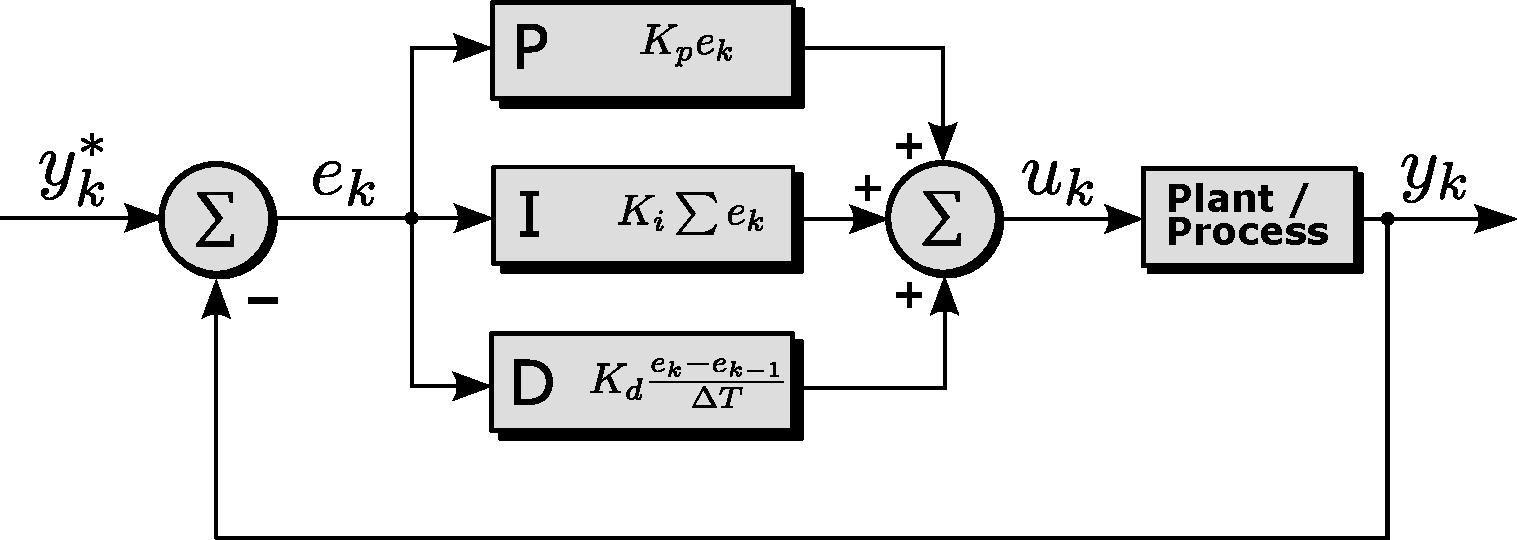
\includegraphics[width=10cm]{fig/lec01/Control_Loop.pdf}
	\caption{Classical PID control loop with scalar quantities (derivative of \href{https://en.wikipedia.org/wiki/PID_controller}{www.wikipedia.org}, by Arturo Urquizo \href{https://creativecommons.org/licenses/by-sa/3.0/deed.en}{CC BY-SA 3.0})}
	\label{fig:Control_Loop_PID}
\end{figure}
}

%%%%%%%%%%%%%%%%%%%%%%%%%%%%%%%%%%%%%%%%%%%%%%%%%%%%%%%%%%%%%
%% Stochastic policy example %%
%%%%%%%%%%%%%%%%%%%%%%%%%%%%%%%%%%%%%%%%%%%%%%%%%%%%%%%%%%%%%
\frame{\frametitle{Stochastic Policy Example}
\onslide<1->Task: Two-player game of extended rock-paper-scissors 
\begin{itemize}
	\onslide<2->\item A deterministic policy can be easily exploited by the opponent.
	\onslide<3->\item	A uniform random policy would be instead unpredictable\\(assuming an ideal random number generator).
\end{itemize}

\onslide<1->
\begin{figure}
	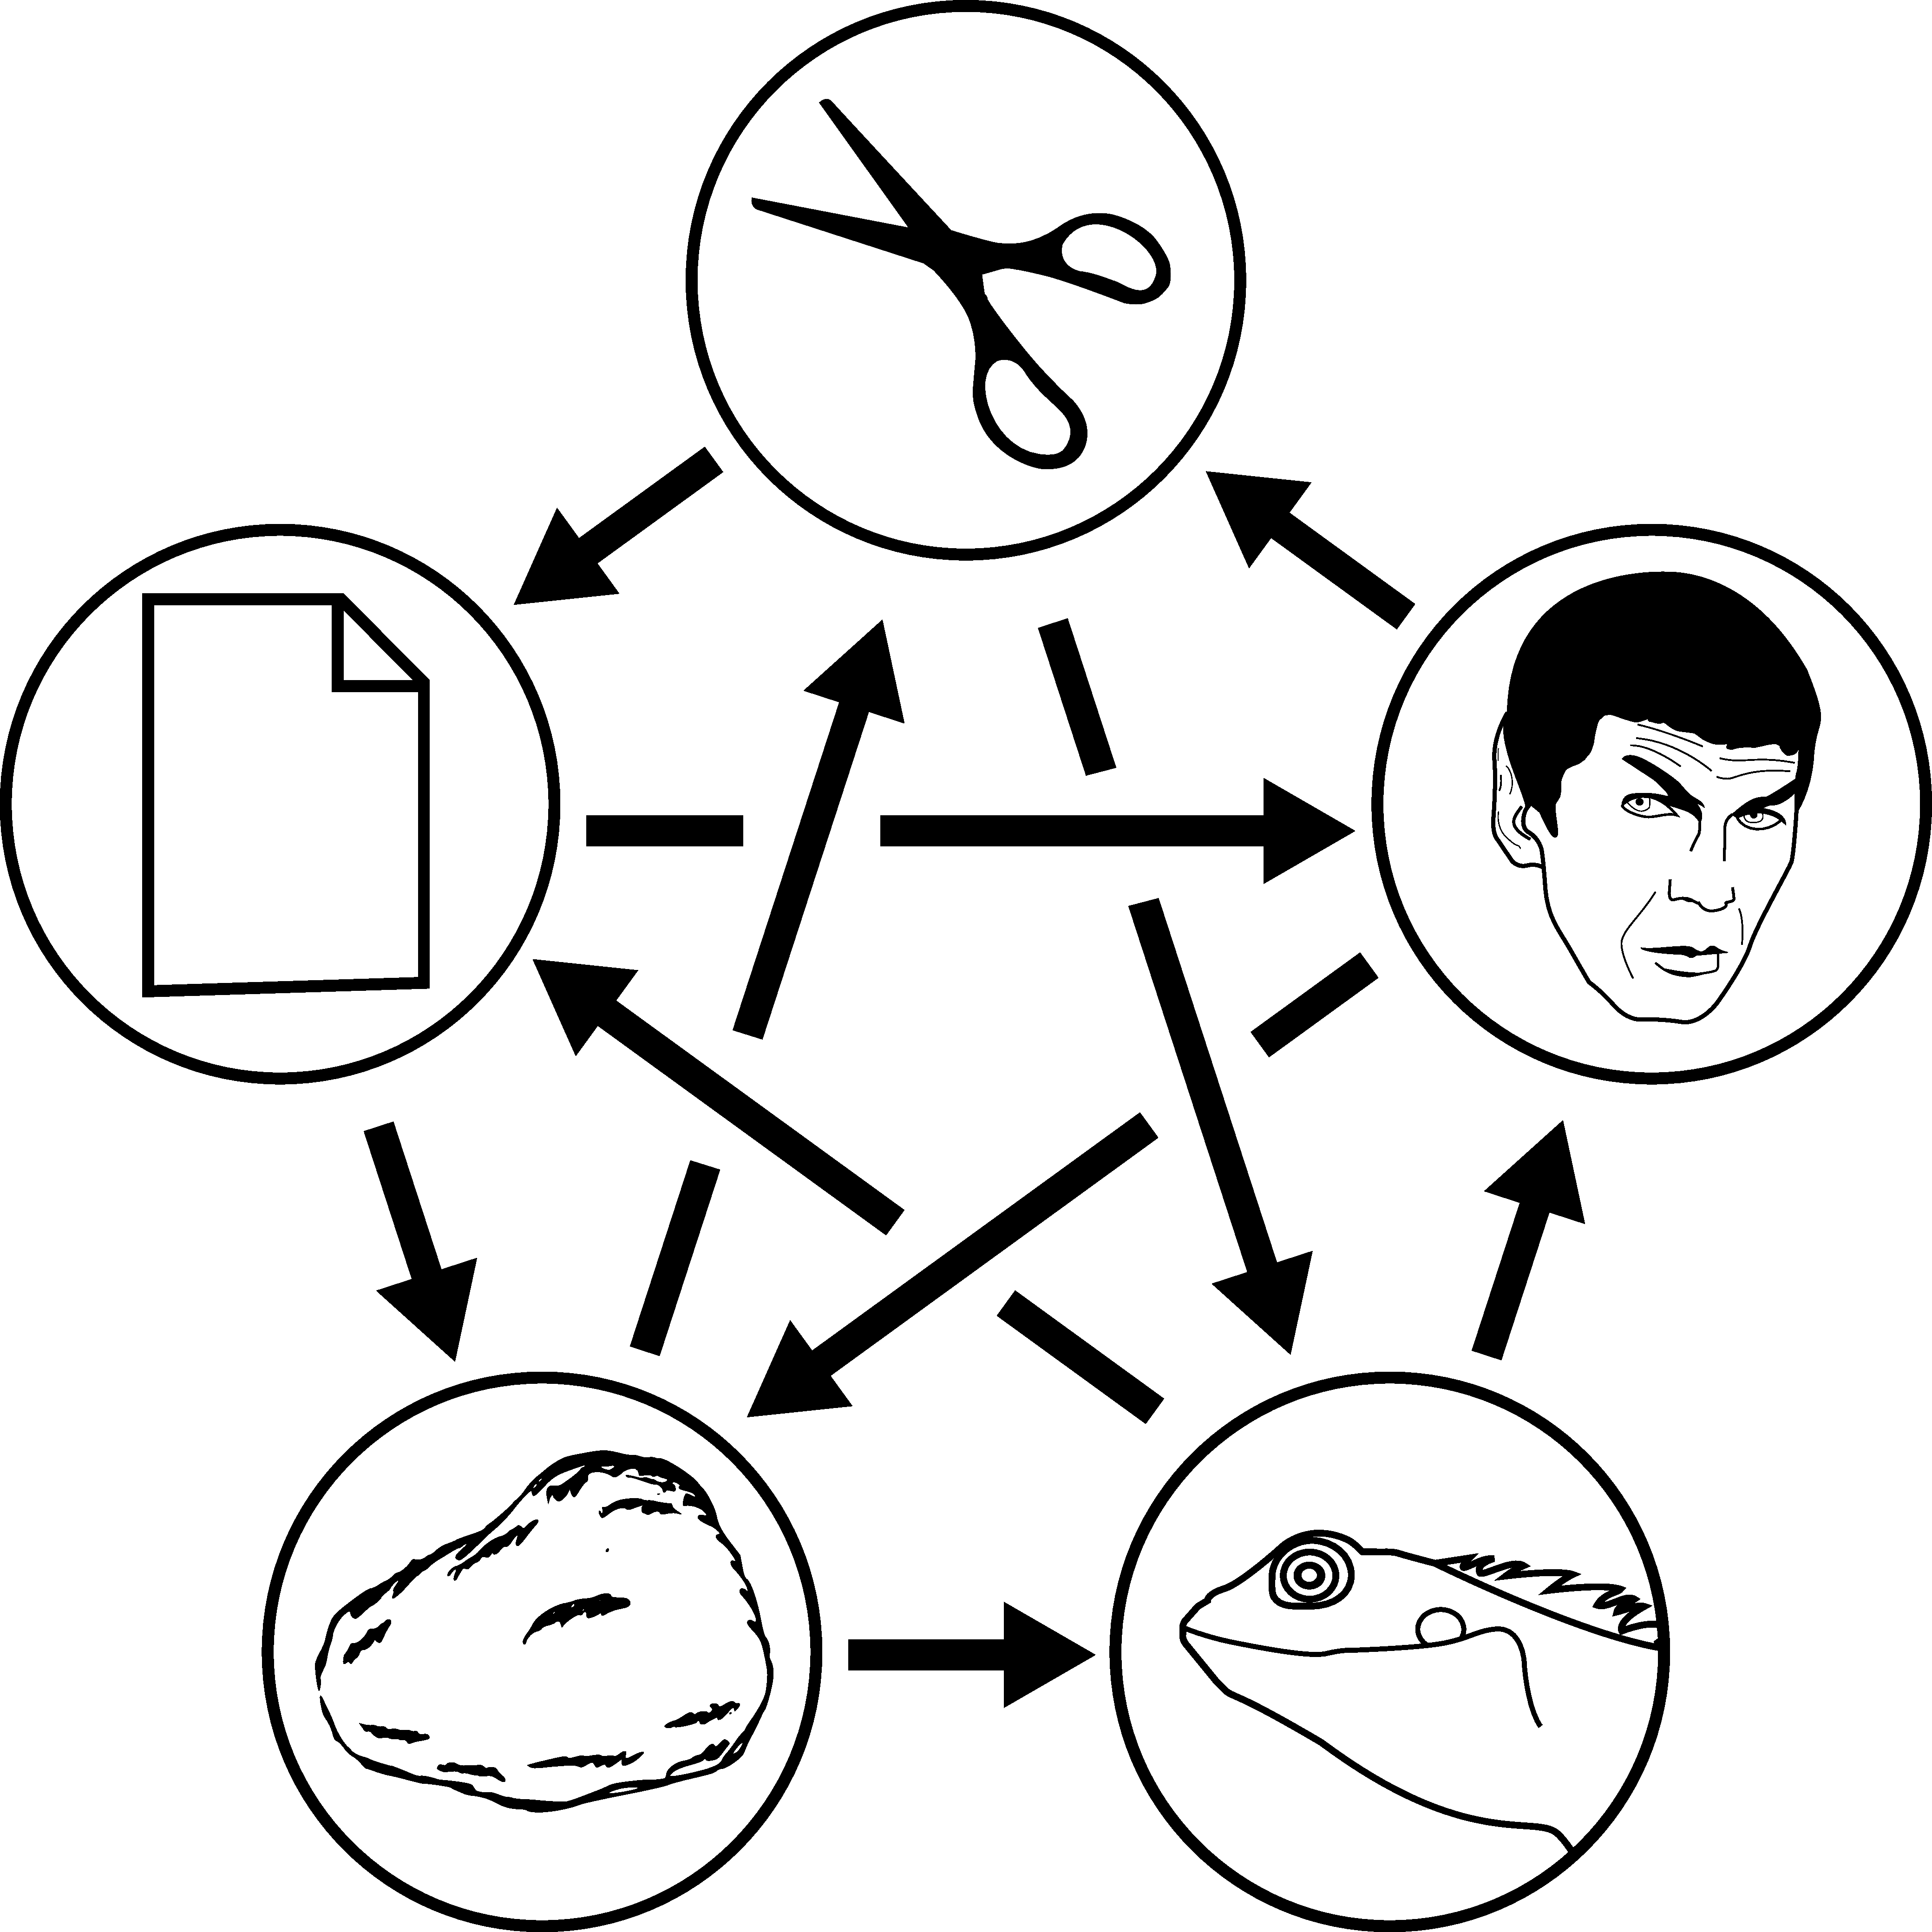
\includegraphics[width=4.3cm]{fig/lec01/Rock_paper_scissors_lizard_spock.pdf}
	\caption{Rock paper scissors lizard Spock game mechanics\\(source: \href{https://commons.wikimedia.org/wiki/File:Rock_paper_scissors_lizard_spock.svg}{www.wikipedia.org},  by \href{https://en.wikipedia.org/wiki/User:Diriector_Doc}{Diriector Doc} \href{https://creativecommons.org/licenses/by-sa/4.0/deed.en}{CC BY-SA 4.0})}
	\label{fig:Rock_paper_scissors_lizard_spock}
\end{figure}
}

%%%%%%%%%%%%%%%%%%%%%%%%%%%%%%%%%%%%%%%%%%%%%%%%%%%%%%%%%%%%%
%% Value function %%
%%%%%%%%%%%%%%%%%%%%%%%%%%%%%%%%%%%%%%%%%%%%%%%%%%%%%%%%%%%%%
\frame{\frametitle{Value Functions}
\begin{itemize}
	\item The \hl{state-value function} is the expected return being in state $\bm{x}_k$ following a policy $\bm{\pi}$: $v_\pi(\bm{x}_k)$.
	\pause
	\item Assuming an MDP problem structure the state-value function is
	\begin{equation}
	\label{eq:state_value_lec01}
		v_\pi(\bm{x}_k) = \El{G_k|\bm{X}_k=\bm{x}_k}{\pi}=\El{\left. \sum_{i=0}^\infty \gamma^i R_{k+i+1}\right|\bm{x}_k}{\pi}.
	\end{equation}
	\pause
\item The \hl{action-value function} is the expected return being in state $\bm{x}_k$ taken an action $\bm{u}_k$ and, thereafter, following a policy $\bm{\pi}$: $q_\pi(\bm{x}_k, \bm{u}_k)$.
\pause
	\item Assuming an MDP problem structure the action-value function is
\end{itemize}
	\begin{equation}
		q_\pi(\bm{x}_k,\bm{u}_k) = \El{G_k|\bm{X}_k=\bm{x}_k, \bm{U}_k=\bm{u}_k}{\pi}=\El{\left.\sum_{i=0}^\infty \gamma^i R_{k+i+1}\right|\bm{x}_k, \bm{u}_k}{\pi}.
	\end{equation}\pause
\begin{itemize}
	\item A key task in RL is to estimate $v_\pi(\bm{x}_k)$ and $q_\pi(\bm{x}_k,\bm{u}_k)$ based on sampled data.
\end{itemize}
}

%%%%%%%%%%%%%%%%%%%%%%%%%%%%%%%%%%%%%%%%%%%%%%%%%%%%%%%%%%%%%
%% Model %%
%%%%%%%%%%%%%%%%%%%%%%%%%%%%%%%%%%%%%%%%%%%%%%%%%%%%%%%%%%%%%
\frame{\frametitle{Model}
\begin{itemize}
	\item A \hl{model} predicts what will happen inside an environment.\pause
	\item That could be a state model $\bm{\mathcal{P}}$:
	\begin{equation}
		\bm{\mathcal{P}} = \Pb{\bm{X}_{k+1}=\bm{x}_{k+1}|\bm{X}_k=\bm{x}_k, \bm{U}_k=\bm{u}_k}\,.
	\end{equation}
	\pause
	\item Or a reward model $\mathcal{R}$:
	\begin{equation}
		\mathcal{R} = \Pb{R_{k+1}=r_{k+1}|\bm{X}_k=\bm{x}_k, \bm{U}_k=\bm{u}_k}\,.
	\end{equation}
	\pause
	\item In general, those models could be stochastic (as denoted above) but in some problems relax to a deterministic form.\pause
	\item Using data in order to fit a model is a learning problem of its own and often called \hl{system identification}.
\end{itemize}
}

%%%%%%%%%%%%%%%%%%%%%%%%%%%%%%%%%%%%%%%%%%%%%%%%%%%%%%%%%%%%%
%% Exploration and Exploitation %%
%%%%%%%%%%%%%%%%%%%%%%%%%%%%%%%%%%%%%%%%%%%%%%%%%%%%%%%%%%%%%
\frame{\frametitle{Exploration and Exploitation}
\begin{itemize}
	\item In RL the environment is initially unknown. How to act optimal?
	\item \hl{Exploration}: Find out more about the environment.
	\item \hl{Exploitation}: Maximize current reward using limited
	information.\pause
	\item Trade-off problem: what's the best split between both strategies?
\end{itemize}	
\begin{figure}
	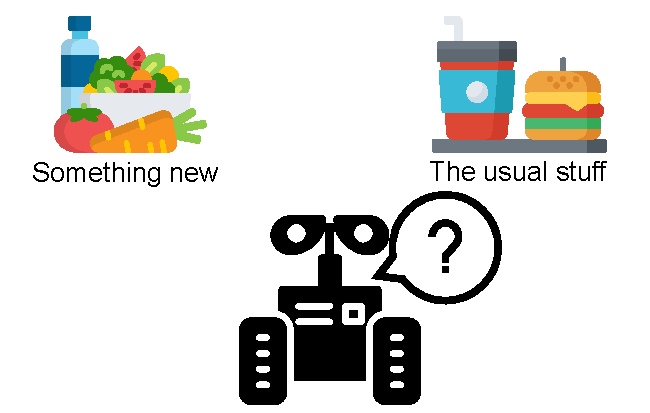
\includegraphics[width=7cm]{fig/lec01/Exploration_Exploitation.pdf}
	\caption{The exploration exploitation dilemma}
	\label{fig:Exploration_Exploitation}
\end{figure}
}

%%%%%%%%%%%%%%%%%%%%%%%%%%%%%%%%%%%%%%%%%%%%%%%%%%%%%%%%%%%%%%%%%%
\section{Main Categories of Reinforcement Learning Algorithms} 
%%%%%%%%%%%%%%%%%%%%%%%%%%%%%%%%%%%%%%%%%%%%%%%%%%%%%%%%%%%%%%%%%%
\begin{frame}
\frametitle{Table of Contents}
\tableofcontents[currentsection]
\end{frame}

%%%%%%%%%%%%%%%%%%%%%%%%%%%%%%%%%%%%%%%%%%%%%%%%%%%%%%%%%%%%%
%% Maze Example%%
%%%%%%%%%%%%%%%%%%%%%%%%%%%%%%%%%%%%%%%%%%%%%%%%%%%%%%%%%%%%%
\frame{\frametitle{Maze Example}
\begin{minipage}[c]{0.5\linewidth}
	\begin{figure}
		
\includegraphics[width=6cm]{fig/lec01/Maze_Basic.pdf}
		\caption{Maze setup\\ \SilverLectureSource}
		\label{fig:Maze_Basic}
	\end{figure}
\end{minipage}
\hfill
\begin{minipage}[c]{0.47\linewidth}
\vspace{0.3cm}
Problem statement:
	\begin{itemize}
		\item Reward: $r_k=-1$ 
		\item At goal: episode termination
		\item Actions: $u_k\in\left\{N, E, S, W\right\}$
		\item State: Agent's location
		\item Deterministic problem (no stochastic influences)
	\end{itemize}
\end{minipage}
}

%%%%%%%%%%%%%%%%%%%%%%%%%%%%%%%%%%%%%%%%%%%%%%%%%%%%%%%%%%%%%
%% Maze Policy%%
%%%%%%%%%%%%%%%%%%%%%%%%%%%%%%%%%%%%%%%%%%%%%%%%%%%%%%%%%%%%%
\frame{\frametitle{Maze Example: RL-Solution by Policy}
\begin{minipage}[c]{0.55\linewidth}
	\begin{figure}
		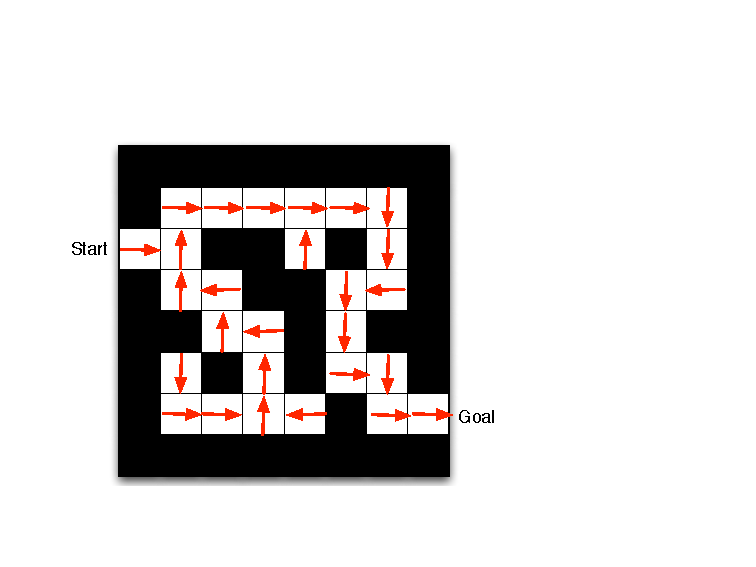
\includegraphics[width=6cm]{fig/lec01/Maze_Policy.pdf}
		\caption{Arrows represent policy $\pi(x_k)$ \SilverLectureSource}
		\label{fig:Maze_Policy}
	\end{figure}
\end{minipage}
\hfill
\begin{minipage}[c]{0.43\linewidth}
Key characteristics:
	\begin{itemize}
		\item For any state there is a direct action command.
		\item The policy is explicitly available.
	\end{itemize}
\end{minipage}
}

%%%%%%%%%%%%%%%%%%%%%%%%%%%%%%%%%%%%%%%%%%%%%%%%%%%%%%%%%%%%%
%% Maze Value%%
%%%%%%%%%%%%%%%%%%%%%%%%%%%%%%%%%%%%%%%%%%%%%%%%%%%%%%%%%%%%%
\frame{\frametitle{Maze Example: RL-Solution by Value Function}
\begin{minipage}[c]{0.55\linewidth}
	\begin{figure}
		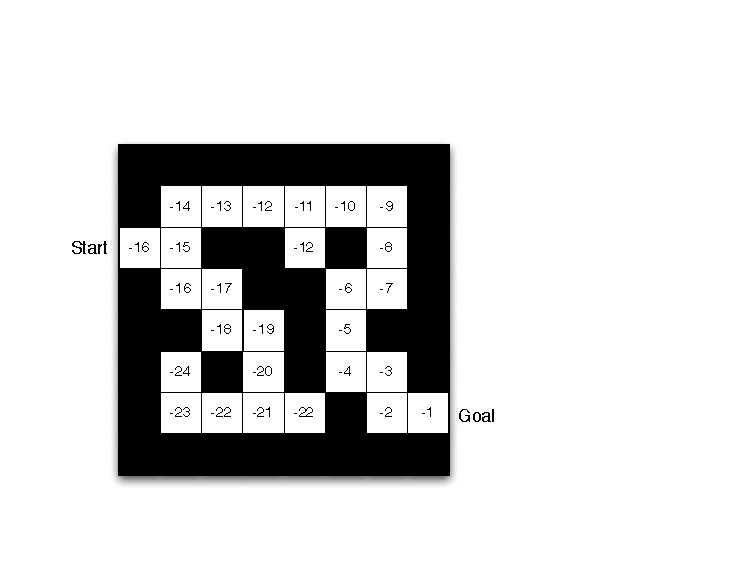
\includegraphics[width=6cm]{fig/lec01/Maze_Value.pdf}
		\caption{Numbers represent value $v_{\pi}(x_k)$ \SilverLectureSource}
		\label{fig:Maze_Value}
	\end{figure}
\end{minipage}
\hfill
\begin{minipage}[c]{0.43\linewidth}
Key characteristics:
	\begin{itemize}
		\item The agent evaluates neighboring maze positions by their value.
		\item The policy is only implicit.
	\end{itemize}
\end{minipage}
}

%%%%%%%%%%%%%%%%%%%%%%%%%%%%%%%%%%%%%%%%%%%%%%%%%%%%%%%%%%%%%
%% Maze Model%%
%%%%%%%%%%%%%%%%%%%%%%%%%%%%%%%%%%%%%%%%%%%%%%%%%%%%%%%%%%%%%
\frame{\frametitle{Maze Example: RL-Solution by Model Evaluation}
\begin{minipage}[c]{0.55\linewidth}
	\begin{figure}
		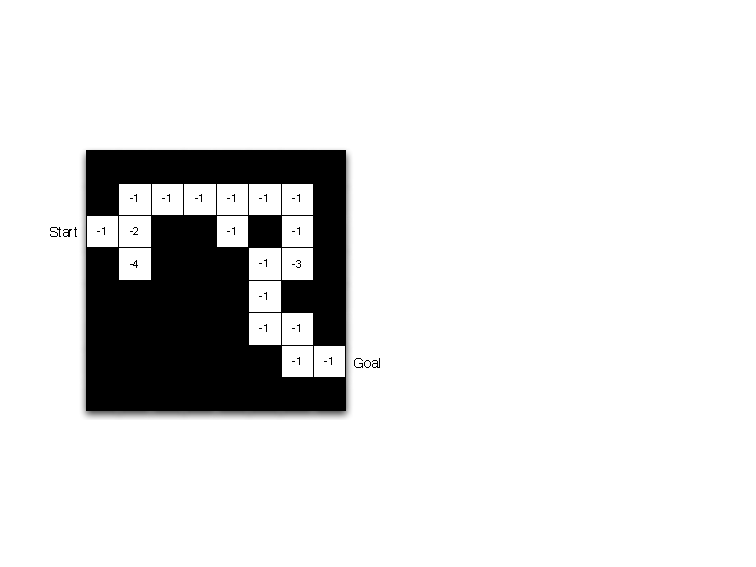
\includegraphics[width=6cm]{fig/lec01/Maze_Model.pdf}
		\caption{Grid layout represents state model $\mathcal{P}$ and numbers depict the estimate by the reward model $\mathcal{R}$.  \SilverLectureSource}
		\label{fig:Maze_Model}
	\end{figure}
\end{minipage}
\hfill
\begin{minipage}[c]{0.43\linewidth}
Key characteristics:
	\begin{itemize}
		\item Agent uses internal model of the environment. 
		\item The model is only an estimate (inaccurate, incomplete).
		\item The agent interacts with the model before taking the next action (e.g., by numerical optimizers).
	\end{itemize}
\end{minipage}
}

%%%%%%%%%%%%%%%%%%%%%%%%%%%%%%%%%%%%%%%%%%%%%%%%%%%%%%%%%%%%%
%% RL Agent Taxonomy%%
%%%%%%%%%%%%%%%%%%%%%%%%%%%%%%%%%%%%%%%%%%%%%%%%%%%%%%%%%%%%%
\frame{\frametitle{RL Agent Taxonomy}
\begin{figure}
	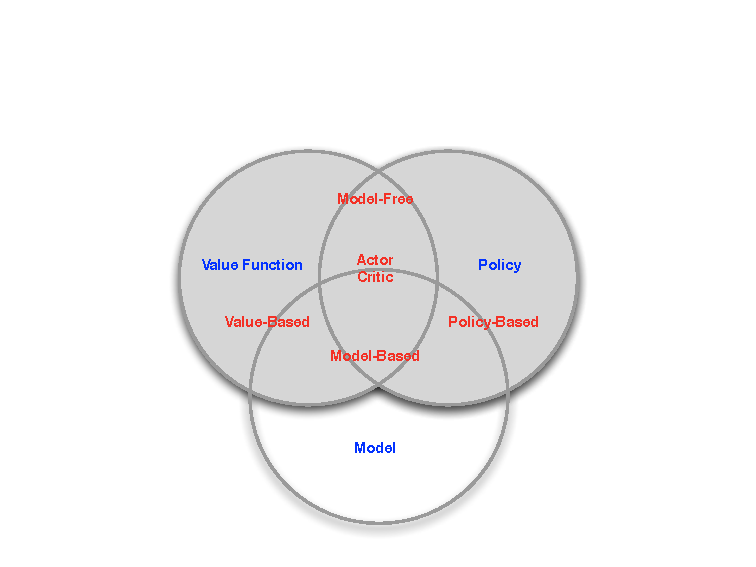
\includegraphics[width=7cm]{fig/lec01/RL_Agent_Taxonomy.pdf}
	\caption{Main categories of reinforcement learning algorithms\\  \SilverLectureSource}
	\label{fig:RL_Agent_Taxonomy}
\end{figure}
}


%%%%%%%%%%%%%%%%%%%%%%%%%%%%%%%%%%%%%%%%%%%%%%%%%%%%%%%%%%%%%%%%%%
\section{Small Comparison to Model Predictive Control} 
%%%%%%%%%%%%%%%%%%%%%%%%%%%%%%%%%%%%%%%%%%%%%%%%%%%%%%%%%%%%%%%%%%
\begin{frame}
\frametitle{Table of Contents}
\tableofcontents[currentsection]
\end{frame}

%%%%%%%%%%%%%%%%%%%%%%%%%%%%%%%%%%%%%%%%%%%%%%%%%%%%%%%%%%%%%
%% RL Agent Taxonomy%%
%%%%%%%%%%%%%%%%%%%%%%%%%%%%%%%%%%%%%%%%%%%%%%%%%%%%%%%%%%%%%
\frame{\frametitle{RL vs. Planning}
Two fundamental solutions to sequential decision making:
\begin{itemize}
	\item Reinforcement learning:
	\begin{itemize}
		\item The environment is initially unknown.
		\item The agents interacts with the environment.
		\item The policy is improved based on environment feedback (reward).
	\end{itemize}
	\pause
	\item Planning:
	\begin{itemize}
		\item An a priori environment model exists.
		\item The agents interacts with its own model.
		\item The policy is improved based on the model feedback ('virtual reward').
	\end{itemize}
\end{itemize}
\pause
\begin{block}{Remark on learning and planning}
Above the two extreme cases are confronted: 
\begin{itemize}
	\item RL = only learning without using available pre-knowledge.
	\item Planning = iterating on a model without improving it based on data. 
\end{itemize}
\pause
Can this lead to efficient and optimal solutions?
\end{block}
}

%%%%%%%%%%%%%%%%%%%%%%%%%%%%%%%%%%%%%%%%%%%%%%%%%%%%%%%%%%%%%
%% Problem Statement MPC/Rl%%
%%%%%%%%%%%%%%%%%%%%%%%%%%%%%%%%%%%%%%%%%%%%%%%%%%%%%%%%%%%%%
\frame{\frametitle{Problem Reconsideration}
The reward hypothesis in \theoref{theo:reward_hypo} is basically an \hl{infinite-horizon optimal control} problem (with $r_k$ interpreted as costs):
\begin{equation}
	v_k^* = \min_{\bm{u}_k} \sum_{i=1}^\infty r_{k+i} (\bm{x}_{k+i}, \bm{u}_{k+i})\,.
\end{equation}
\pause
For certain cases closed-form solutions can be found, e.g., a LTI system with quadratic costs and no further constraints can be optimally controlled by a linear-quadratic regulator (LQR). However, for arbitrary cases that is not possible and one relaxes the problem to a \hl{finite-horizon optimal control} problem:   
\begin{equation}
	v_k^* = \min_{\bm{u}_k} \sum_{i=1}^{N_p} r_{k+i} (\bm{x}_{k+i}, \bm{u}_{k+i})\,.
\end{equation}
\pause
Here, an internal model $\bm{x}_{k+1}=\bm{f}(\bm{x}_k,\bm{u}_k)$ is utilized to predict the system behavior for $N_p$ future steps. This \hl{model predictive control} (MPC) approach can be solved using numeric solvers. 
}

%%%%%%%%%%%%%%%%%%%%%%%%%%%%%%%%%%%%%%%%%%%%%%%%%%%%%%%%%%%%%
%% Constraints MPC%%
%%%%%%%%%%%%%%%%%%%%%%%%%%%%%%%%%%%%%%%%%%%%%%%%%%%%%%%%%%%%%
\frame{\frametitle{MPC and Constraints}
While in RL the desired system behavior must be solely represented by $r_k$, MPC can directly take into account system constraints:
\begin{equation}
	\begin{split}
	v_k^* &= \min_{\bm{u}_k} \sum_{i=1}^{N_p} r_k (\bm{x}_{k+i}, \bm{u}_{k+i})\, ,\\
	s.t. \quad \bm{x}_{k+1}&=\bm{f}(\bm{x}_k,\bm{u}_k), \, \bm{x}_k \in \mathcal{X},\, \bm{u}_k \in \mathcal{U}\,.\\
\end{split}
\end{equation}
\begin{figure}
\centering
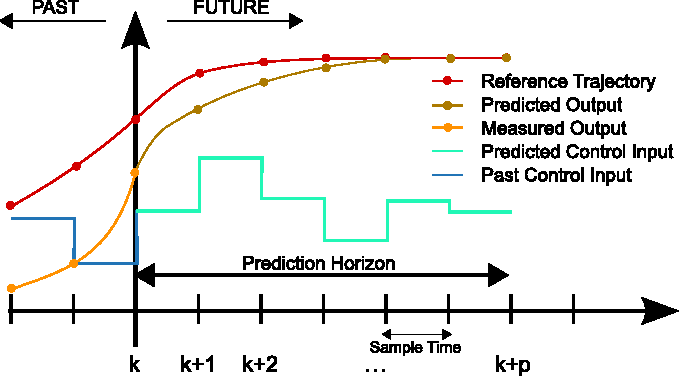
\includegraphics[width=6.5cm]{fig/lec01/MPC.pdf}
\caption{Basic MPC scheme\\(source: \href{https://de.wikipedia.org/wiki/Model_Predictive_Control}{www.wikipedia.org},  by Martin Behrendt \href{https://creativecommons.org/licenses/by-sa/3.0/deed.en}{CC BY-SA 3.0})}
\label{fig:MPC}
\end{figure}
}

%%%%%%%%%%%%%%%%%%%%%%%%%%%%%%%%%%%%%%%%%%%%%%%%%%%%%%%%%%%%%
%% MPC vs RL%%
%%%%%%%%%%%%%%%%%%%%%%%%%%%%%%%%%%%%%%%%%%%%%%%%%%%%%%%%%%%%%
\frame{\frametitle{MPC vs. RL}
\onslide<1->Hence, MPC and RL are two sides of the same coin. Both share the same general goal (optimal decision making), but follow their own philosophy:  
\begin{table}
	\centering
		\begin{tabular}{lll}
			Property & MPC & RL\\
			\hline
			\onslide<1->Objective 									& minimize costs 									& maximize return  \\
			\onslide<2->A priori model 							& required \xmark 								& not required \cmark \\
			\onslide<3->Pre-knowledge integration 	& easy \cmark 										& rather complex \xmark \\
			\onslide<4->Constraint handling					& inherent \cmark 								&	only indirect \xmark \\
			\onslide<5->Adaptivity									& requires add-ons \xmark 				&	inherent \cmark \\
			\onslide<6->Online complexity						& high \xmark 										&	it depends \cmark/\xmark \\
			\onslide<7->Stability theory						& mature \cmark 									&	immature \xmark \\
		\end{tabular}
	\onslide<1->\caption{Key differences on MPC vs. RL\\(based on D. G�rges, \textit{Relations between Model Predictive Control and Reinforcement Learning}, IFAC PapersOnine 50-1, pp. 4920-4928, 2017)}
	\label{tab:KeyDifferences}
\end{table}
}

%%%%%%%%%%%%%%%%%%%%%%%%%%%%%%%%%%%%%%%%%%%%%%%%%%%%%%%%%%%%%
%% Summary %%
%%%%%%%%%%%%%%%%%%%%%%%%%%%%%%%%%%%%%%%%%%%%%%%%%%%%%%%%%%%%%
\begin{frame}
\frametitle{Summary: What You've Learned Today}
\begin{itemize}
	\item Understanding the role of RL in machine learning and optimal sequential decision making. \pause
	\item Become acquainted with the basic RL interaction loop (agent, environment, interpreter). \pause
	\item Finding your way around the basic RL vocabulary. \pause
	\item Internalize the significance of proper reward formulations (design parameter). \pause
	\item Differentiate solution ideas on how to retrieve an optimal agent behavior (policy). \pause
	\item Delimit RL towards model predictive control as a sequential decision making alternative. 
\end{itemize}
\end{frame}

%%%%%%%%%%%%%%%%%%%%%%%%%%%%%%%%%%%%%%%%%%%%%%%%%%%%%%%%%%%%%
%% Final Slide %%
%%%%%%%%%%%%%%%%%%%%%%%%%%%%%%%%%%%%%%%%%%%%%%%%%%%%%%%%%%%%%
\frame{\frametitle{The End for Today}
\begin{figure}

\includegraphics[width=10cm]{fig/lec01/Dilbert.jpg}
\end{figure}
\vspace{1cm}
\centering
Thanks for your attention and have a nice week!
}
\part{Lecture 02: Markov Decision Processes}
\title[RL Lecture 02]{Lecture 02: Markov Decision Processes}  
\date{}  
\frame{\titlepage} 

%%%%%%%%%%%%%%%%%%%%%%%%%%%%%%%%%%%%%%%%%%%%%%%%%%%%%%%%%%%%%
%% Preface / Motivation %%
%%%%%%%%%%%%%%%%%%%%%%%%%%%%%%%%%%%%%%%%%%%%%%%%%%%%%%%%%%%%%
\frame{\frametitle{Preface}
\begin{itemize}
	\onslide<2->\item Markov decision processes (MDP) are a \hl{mathematically idealized form of RL problems}.
	\onslide<2->\item They allow precise theoretical statements (e.g., on optimal solutions).
	\onslide<2->\item They deliver insights into suitable RL algorithms since many real-world problems can be abstracted as MDPs. 
	\onslide<3->\item In the following \hl{we'll focus on}:
	\onslide<3->\begin{itemize}
		\item fully observable MDPs (i.e., $\bm{x}_k=\bm{y}_k$) and 
		\item finite MDPs (i.e., finite number of states \& actions).
	\end{itemize}
\end{itemize}
\hfill
\onslide<1->\begin{table}
	\centering
		\begin{tabular}{|M{0.5cm}|M{1cm}||M{3cm}|M{3cm}|}
		\cline{3-4}
			\multicolumn{2}{c||}{\multirow{2}{*}{}}& \multicolumn{2}{c|}{All states observable?}\\
			\cline{3-4}
			\multicolumn{2}{c||}{} & Yes & No\\
			\hline\hline
			 \multirow{2}{*}{\rotatebox{90}{Actions?}} & No & Markov chain &Hidden Markov model\\
			\cline{2-4}
			& Yes & Markov decision process (MDP) & Partially observable MDP\\
			\hline
		\end{tabular}
	\caption{Different Markov models}
	\label{tab:DifferentMarkovModels}
\end{table}
}

%%%%%%%%%%%%%%%%%%%%%%%%%%%%%%%%%%%%%%%%%%%%%%%%%%%%%%%%%%%%%
%% Remark: Scalar and Vectorial State/Action Representation %%
%%%%%%%%%%%%%%%%%%%%%%%%%%%%%%%%%%%%%%%%%%%%%%%%%%%%%%%%%%%%%
\frame{\frametitle{Scalar and Vectorial Representations in Finite MDPs}
\begin{itemize}
	\onslide<1->\item The position of a chess piece can be represented in two ways:
	\begin{itemize}
		\onslide<1->\item Vectorial: $\bm{x}=\begin{bmatrix}x_h & x_v\end{bmatrix}\T$, i.e., a two-element vector with horizontal and vertical information (e.g., $\bm{x}=\begin{bmatrix}c & 1 \end{bmatrix}\T$) or
		\onslide<2->\item \hl{Scalar: simple enumeration of all available positions (e.g., $x=3$).}
	\end{itemize}
	\onslide<3->\item Both ways represent the same amount of information and can be easily converted into each other.
	\onslide<3->\item For sake of readability \hl{we will stick to the scalar representation of states and actions in finite MDPs} whenever possible.
\end{itemize}
\onslide<1->\begin{figure}		
	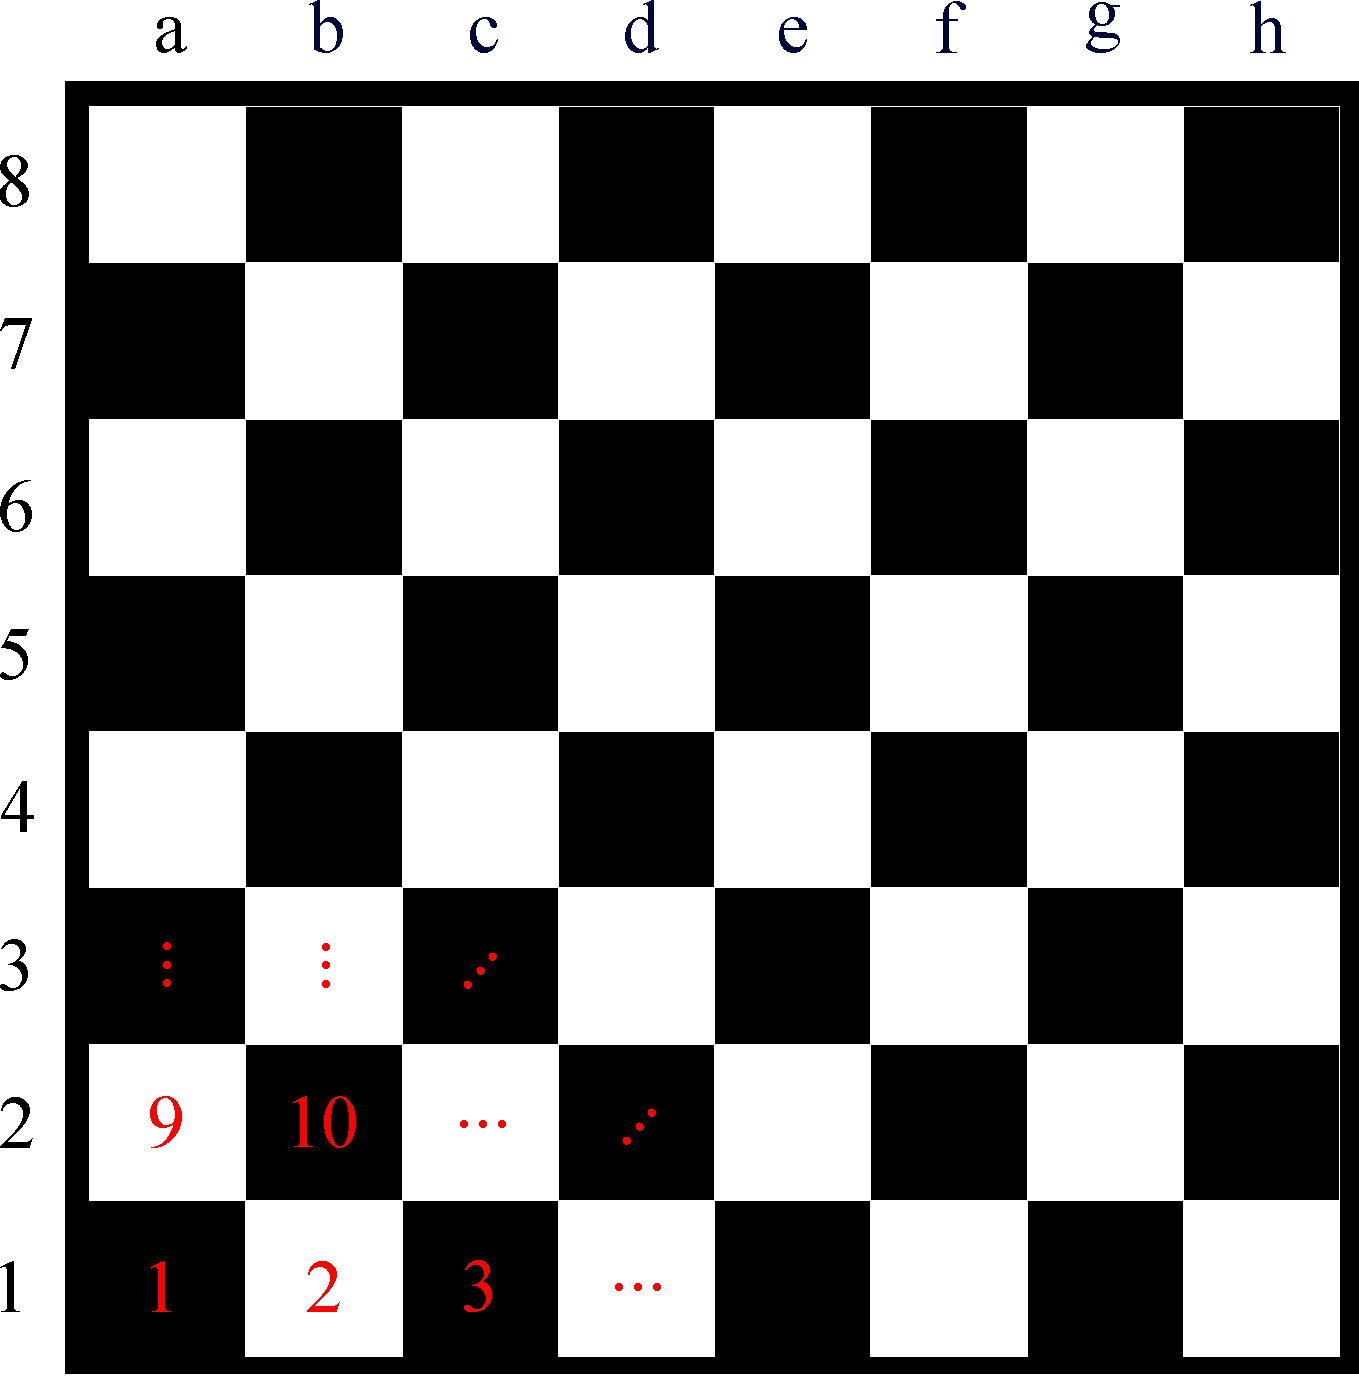
\includegraphics[width=4cm]{fig/lec02/Chess_Board.pdf}
\end{figure}
}

\frame{\frametitle{Table of Contents}\tableofcontents} 

%%%%%%%%%%%%%%%%%%%%%%%%%%%%%%%%%%%%%%%%%%%%%%%%%%%%%%%%%%%%%%%%%%
\section{Finite Markov Chains} 
%%%%%%%%%%%%%%%%%%%%%%%%%%%%%%%%%%%%%%%%%%%%%%%%%%%%%%%%%%%%%%%%%%

%%%%%%%%%%%%%%%%%%%%%%%%%%%%%%%%%%%%%%%%%%%%%%%%%%%%%%%%%%%%%
%% Recap Markov Property %%
%%%%%%%%%%%%%%%%%%%%%%%%%%%%%%%%%%%%%%%%%%%%%%%%%%%%%%%%%%%%%
\frame{\frametitle{Recap on Markov Property}

\begin{block}{Information state}
A state $X_k$ is called an information or Markov state if and only if
\begin{equation}
	\Pb{X_{k+1}|X_k}=\Pb{X_{k+1}|X_0, X_1,\ldots, X_k}\, .
\end{equation}
\end{block}
\pause
\begin{itemize}
	\item History is fully condensed in the sample $X_k$, i.e., $X_{k+1}$ is only depending on $X_k$.
	\item A given system can be fully described by $X_k$.
	\item Further past observations $X_{k-1},X_{k-2},\ldots$ are irrelevant.
\end{itemize}
}

%%%%%%%%%%%%%%%%%%%%%%%%%%%%%%%%%%%%%%%%%%%%%%%%%%%%%%%%%%%%%
%% State Transistion Matrix %%
%%%%%%%%%%%%%%%%%%%%%%%%%%%%%%%%%%%%%%%%%%%%%%%%%%%%%%%%%%%%%
\frame{\frametitle{State Transition Matrix}

\begin{defi}{State transition matrix}{STM}
Given a Markov state $X_k=x$ and its successor $X_{k+1}=x'$ , the \hl{state transition probability} $\forall \left\{x,x'\right\}\in \mathcal{X}$ is defined by the matrix
\begin{equation}
	\bm{\mathcal{P}}_{xx'}=\Pb{X_{k+1}=x'|X_{k}=x} .
\end{equation}
 \end{defi}
\pause
Here,  $\bm{\mathcal{P}}_{xx'}\in\mathbb{R}^{n\times n}$ has the form
\begin{equation*}
	\bm{\mathcal{P}}_{xx'} = \begin{bmatrix} p_{11} & p_{12} & \cdots & p_{1n}\\ p_{21} &  &  & \vdots\\ \vdots & & & \vdots\\ p_{n1} & \cdots & \cdots & p_{nn}\end{bmatrix}
\end{equation*}
with $p_{ij}\in\left\{\mathbb{R}|0 \leq p_{ij} \leq 1 \right\}$ being the specific probability to go from state $x=X_i$ to state $x'=X_j$. Obviously, $\sum_{j} p_{ij}=1 \, \forall i$ must hold.
}

%%%%%%%%%%%%%%%%%%%%%%%%%%%%%%%%%%%%%%%%%%%%%%%%%%%%%%%%%%%%%
%% Markov Chain %%
%%%%%%%%%%%%%%%%%%%%%%%%%%%%%%%%%%%%%%%%%%%%%%%%%%%%%%%%%%%%%
\frame{\frametitle{Markov Chain}

\onslide<1->\begin{defi}{Finite Markov chain}{Markov_chain}
A \hl{finite Markov chain} is a tuple $\left\langle\mathcal{X}, \bm{\mathcal{P}} \right\rangle$ with
\begin{itemize}
	\item $\mathcal{X}$ being a finite set of discrete-time states $X_k\in\mathcal{X}$, 
	\item $\bm{\mathcal{P}}=\bm{\mathcal{P}}_{xx'}=\Pb{X_{k+1}=x'|X_{k}=x}$ is the state transition probability.
\end{itemize}
\end{defi}
\begin{itemize}
	\onslide<2->\item Specific stochastic process model
	\onslide<2->\item Sequence of random variables $X_k, X_{k+1},\ldots$
	\onslide<2->\item 'Memoryless'
	\onslide<3->\item In continuous-time framework: Markov process\only<3->{\footnote[1]{However, this results in a literature nomenclature inconsistency with Markov decision/reward 'processes'.}} 
\end{itemize}
}

%%%%%%%%%%%%%%%%%%%%%%%%%%%%%%%%%%%%%%%%%%%%%%%%%%%%%%%%%%%%%
%% Chapman–Kolmogorov Equation %%
%%%%%%%%%%%%%%%%%%%%%%%%%%%%%%%%%%%%%%%%%%%%%%%%%%%%%%%%%%%%%
\frame{\frametitle{Chapman-Kolmogorov Equation}
Define $\bm{p}_k\in\mathbb{R}^n$ as a \hl{probability row vector} where $p_{i,k}$ gives the probability of being in state $X_k \in\mathcal{X}$ at time-step $k$.  
\begin{defi}{Chapman-Kolmogorov equation for finite Markov chains}{Chapman_Kolmogorov_Equation}
The probability of being in state $X_{k+m}$ at time-step $(k+m)$ starting from state $x_{k}$ is given by:
\begin{equation}
	\bm{p}_{k+m} = \bm{p}_{k}\bm{\mathcal{P}}_{xx'}^{m} .
\end{equation}
\end{defi}
\pause
Hence, for $m\rightarrow\infty$ ('\textit{steady state}') the following equation must hold:
\begin{equation}
	\bm{p} = \bm{p}\bm{\mathcal{P}}_{xx'} .
	\label{eq:Chapman_steady}
\end{equation}
Solving \eqref{eq:Chapman_steady} for $\bm{p}$ given the transition probability $\bm{\mathcal{P}}_{xx'}$ gives insights which states of the Markov chain are visited in the long-run.
}


%%%%%%%%%%%%%%%%%%%%%%%%%%%%%%%%%%%%%%%%%%%%%%%%%%%%%%%%%%%%%
%% Forest Markov Chain Example (1)%%
%%%%%%%%%%%%%%%%%%%%%%%%%%%%%%%%%%%%%%%%%%%%%%%%%%%%%%%%%%%%%
\frame{\frametitle{Example of a Markov Chain (1)}
\begin{minipage}[t]{0.53\linewidth}
		\vspace{0pt}
		\begin{figure}		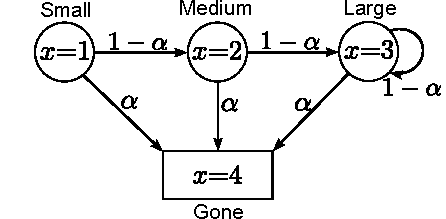
\includegraphics[width=6cm]{fig/lec02/Forest_Markov_Chain.pdf}
		\caption{Forest tree Markov chain}
		\label{fig:Forest_Markov_Chain}
	\end{figure}
\end{minipage}
\begin{minipage}[t]{0.45\linewidth}
\vspace{-0.7cm}
\begin{align*}
  x &= x\in\left\{1,2,3,4\right\}\\
				 &=\left\{\mbox{small},\mbox{medium},\mbox{large},\mbox{gone}\right\}\\[1em]
	\bm{\mathcal{P}} &= \begin{bmatrix}0 & 1-\alpha & 0 & \alpha  \\ 0 & 0 &1-\alpha & \alpha \\ 0 & 0 &1-\alpha & \alpha \\ 0 & 0 & 0 & 1\end{bmatrix}
\end{align*}
\end{minipage}
\begin{itemize}
	\item At $x=1$ a small tree is planted ('starting point').
	\item A tree grows with $(1-\alpha)$ probability.
	\item If it reaches $x=3$ (large) its growth is limited.
	\item With $\alpha$ probability a natural hazard destroys the tree.
	\item The state $x=4$ is terminal ('infinite loop').
\end{itemize}
}

%%%%%%%%%%%%%%%%%%%%%%%%%%%%%%%%%%%%%%%%%%%%%%%%%%%%%%%%%%%%%
%% Forest Markov Chain Example (2)%%
%%%%%%%%%%%%%%%%%%%%%%%%%%%%%%%%%%%%%%%%%%%%%%%%%%%%%%%%%%%%%
\frame{\frametitle{Example of a Markov Chain (2)}
\begin{figure}		
	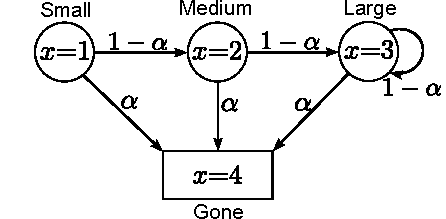
\includegraphics[width=6cm]{fig/lec02/Forest_Markov_Chain.pdf}
\end{figure}
Possible \hl{samples} for the given Markov chain example starting from $x=1$ (small tree):
\begin{itemize}
	\item Small $\rightarrow$ gone
	\item Small $\rightarrow$ medium $\rightarrow$ gone
	\item Small $\rightarrow$ medium $\rightarrow$ large $\rightarrow$ gone
	\item Small $\rightarrow$ medium $\rightarrow$ large $\rightarrow$ large $\rightarrow\ldots$ 
\end{itemize}
}

%%%%%%%%%%%%%%%%%%%%%%%%%%%%%%%%%%%%%%%%%%%%%%%%%%%%%%%%%%%%%
%% Forest Markov Chain Example (3)%%
%%%%%%%%%%%%%%%%%%%%%%%%%%%%%%%%%%%%%%%%%%%%%%%%%%%%%%%%%%%%%
\frame{\frametitle{Example of a Markov Chain (3)}
For $k=0$ the initial state probability is given $\bm{p}_{k=0}=\begin{bmatrix} 1 & 0 & 0 & 0\end{bmatrix}$, i.e., we are in state $x=1$. What is the state probability after $k=1,2,\ldots$ steps with $\alpha = 0.2$?
\begin{alignat*}{2}
	\onslide<2->{\bm{p}_{1}&=\begin{bmatrix}0 & 0.8 & 0 & 0.2\end{bmatrix}&&=\underbrace{\begin{bmatrix} 1 & 0 & 0 & 0\end{bmatrix}}_{\bm{p}_{0}}\underbrace{\begin{bmatrix}0 & 0.8 & 0 & 0.2  \\ 0 & 0 &0.8 & 0.2 \\ 0 & 0 &0.8 & 0.2 \\ 0 & 0 & 0 & 1\end{bmatrix}}_{\bm{\mathcal{P}}}},\\
	\onslide<3->{\bm{p}_{2}&=\begin{bmatrix}0 & 0 & 0.64 & 0.36\end{bmatrix}&&=\underbrace{\begin{bmatrix} 0 & 0.8 & 0 & 0.2\end{bmatrix}}_{\bm{p}_{1}}\underbrace{\begin{bmatrix}0 & 0.8 & 0 & 0.2  \\ 0 & 0 &0.8 & 0.2 \\ 0 & 0 &0.8 & 0.2 \\ 0 & 0 & 0 & 1\end{bmatrix}}_{\bm{\mathcal{P}}}},\\
	\onslide<4->{\bm{p}_{3}&=\begin{bmatrix}0 & 0 & 0.51 & 0.49\end{bmatrix}, &&\quad \bm{p}_{10}=\begin{bmatrix}0 & 0 & 0.11 & 0.89\end{bmatrix},\\
	\bm{p}_{\infty}&=\begin{bmatrix}0 & 0 & 0 & 1\end{bmatrix}.}
\end{alignat*}

}



%%%%%%%%%%%%%%%%%%%%%%%%%%%%%%%%%%%%%%%%%%%%%%%%%%%%%%%%%%%%%%%%%%
\section{Finite Markov Reward Processes} 
%%%%%%%%%%%%%%%%%%%%%%%%%%%%%%%%%%%%%%%%%%%%%%%%%%%%%%%%%%%%%%%%%%
\begin{frame}
\frametitle{Table of Contents}
\tableofcontents[currentsection]
\end{frame}

%%%%%%%%%%%%%%%%%%%%%%%%%%%%%%%%%%%%%%%%%%%%%%%%%%%%%%%%%%%%%
%% Markov Reward Process %%
%%%%%%%%%%%%%%%%%%%%%%%%%%%%%%%%%%%%%%%%%%%%%%%%%%%%%%%%%%%%%
\frame{\frametitle{Markov Reward Process}

\begin{defi}{Finite Markov reward process}{Markov_reward_process}
A \hl{finite Markov reward process (MRP)} is a tuple $\left\langle\mathcal{X}, \bm{\mathcal{P}}, \hl{\mathcal{R}, \gamma} \right\rangle$ with
\begin{itemize}
	\item $\mathcal{X}$ being a finite set of discrete-time states $X_k\in\mathcal{X}$, 
	\item $\bm{\mathcal{P}}=\bm{\mathcal{P}}_{xx'}=\Pb{X_{k+1}=x'|X_{k}=x}$ is the state transition probability,
	\item \hl{$\mathcal{R}$ is a reward function, $\mathcal{R}=\mathcal{R}_x=\E{R_{k+1}|X_k=x_k}$ and} 
	\item \hl{$\gamma$ is a discount factor, $\gamma\in\left\{\mathbb{R}|0 \leq \gamma \leq 1\right\}$}.
\end{itemize}
\end{defi}
\pause
\begin{itemize}
	\item Markov chain extended with rewards \pause
	\item Still an autonomous stochastic process without specific inputs \pause
	\item Reward $R_{k+1}$ only depends on state $X_k$
\end{itemize}
}

%%%%%%%%%%%%%%%%%%%%%%%%%%%%%%%%%%%%%%%%%%%%%%%%%%%%%%%%%%%%%
%% Forest Markov Reward Process %%
%%%%%%%%%%%%%%%%%%%%%%%%%%%%%%%%%%%%%%%%%%%%%%%%%%%%%%%%%%%%%
\frame{\frametitle{Example of a Markov Reward Process}
\begin{figure}		
	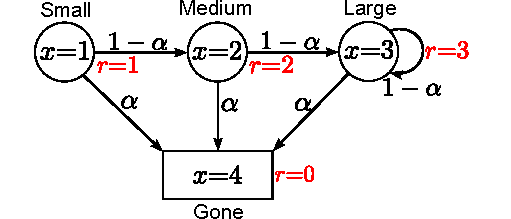
\includegraphics[width=10cm]{fig/lec02/Forest_Markov_Reward_Process.pdf}
	\caption{Forest Markov reward process}
	\label{fig:Forest_Markov_Reward_Process}
\end{figure}

\begin{itemize}
	\item Growing larger trees is rewarded, since it will be
	\begin{itemize}
		\item appreciated by hikers and
		\item useful for wood production.
	\end{itemize}
	\item Loosing a tree due to a hazard is unrewarded.
\end{itemize}
}

%%%%%%%%%%%%%%%%%%%%%%%%%%%%%%%%%%%%%%%%%%%%%%%%%%%%%%%%%%%%%
%% Recap Return %%
%%%%%%%%%%%%%%%%%%%%%%%%%%%%%%%%%%%%%%%%%%%%%%%%%%%%%%%%%%%%%
\frame{\frametitle{Recap on Return}

\begin{block}{Return}
The return $G_k$ is the total discounted reward starting from step $k$ onwards. For \hl{episodic tasks} it becomes the finite series
\begin{equation}
	G_k = R_{k+1} + \gamma R_{k+2} + \gamma^2 R_{k+3} + \cdots = \sum_{i=0}^N \gamma^i R_{k+i+1}  	
\end{equation}
terminating at step $N$ while it is an infinite series for \hl{continuing tasks}	
\begin{equation}
	G_k = R_{k+1} + \gamma R_{k+2} + \gamma^2 R_{k+3} + \cdots = \sum_{i=0}^\infty \gamma^i R_{k+i+1}\, .  	
\end{equation}
\end{block}
\begin{itemize}
	\item The discount $\gamma$ represents the value of future rewards.
\end{itemize}
}

%%%%%%%%%%%%%%%%%%%%%%%%%%%%%%%%%%%%%%%%%%%%%%%%%%%%%%%%%%%%%
%% Remark on notation: Episodic and Continuing Tasks %%
%%%%%%%%%%%%%%%%%%%%%%%%%%%%%%%%%%%%%%%%%%%%%%%%%%%%%%%%%%%%%
\frame{\frametitle{Remark on Notation: Episodic and Continuing Tasks}
\begin{itemize}
	\item In episodic tasks there is not only one (long/infinite) sequence of time steps.
	\item Instead there is a sequence of time steps of an arbitrary episode $j$.
	\begin{itemize}
		\item Formally: $X_{k,j},U_{k,j}, R_{k,j},\ldots$ 
	\end{itemize}
	\onslide<2->{
	\item Nevertheless, to increase the readability the episode index is normally dropped in this course:
	\begin{itemize}
		\item Simplified: $X_{k}\leftarrow X_{k,j},U_{k}\leftarrow U_{k,j}, R_{k}\leftarrow R_{k,j},\ldots$ 
	\end{itemize}
	\item Only in certain cases the episode indexing will be re-activated.
\end{itemize}}
\begin{figure}
	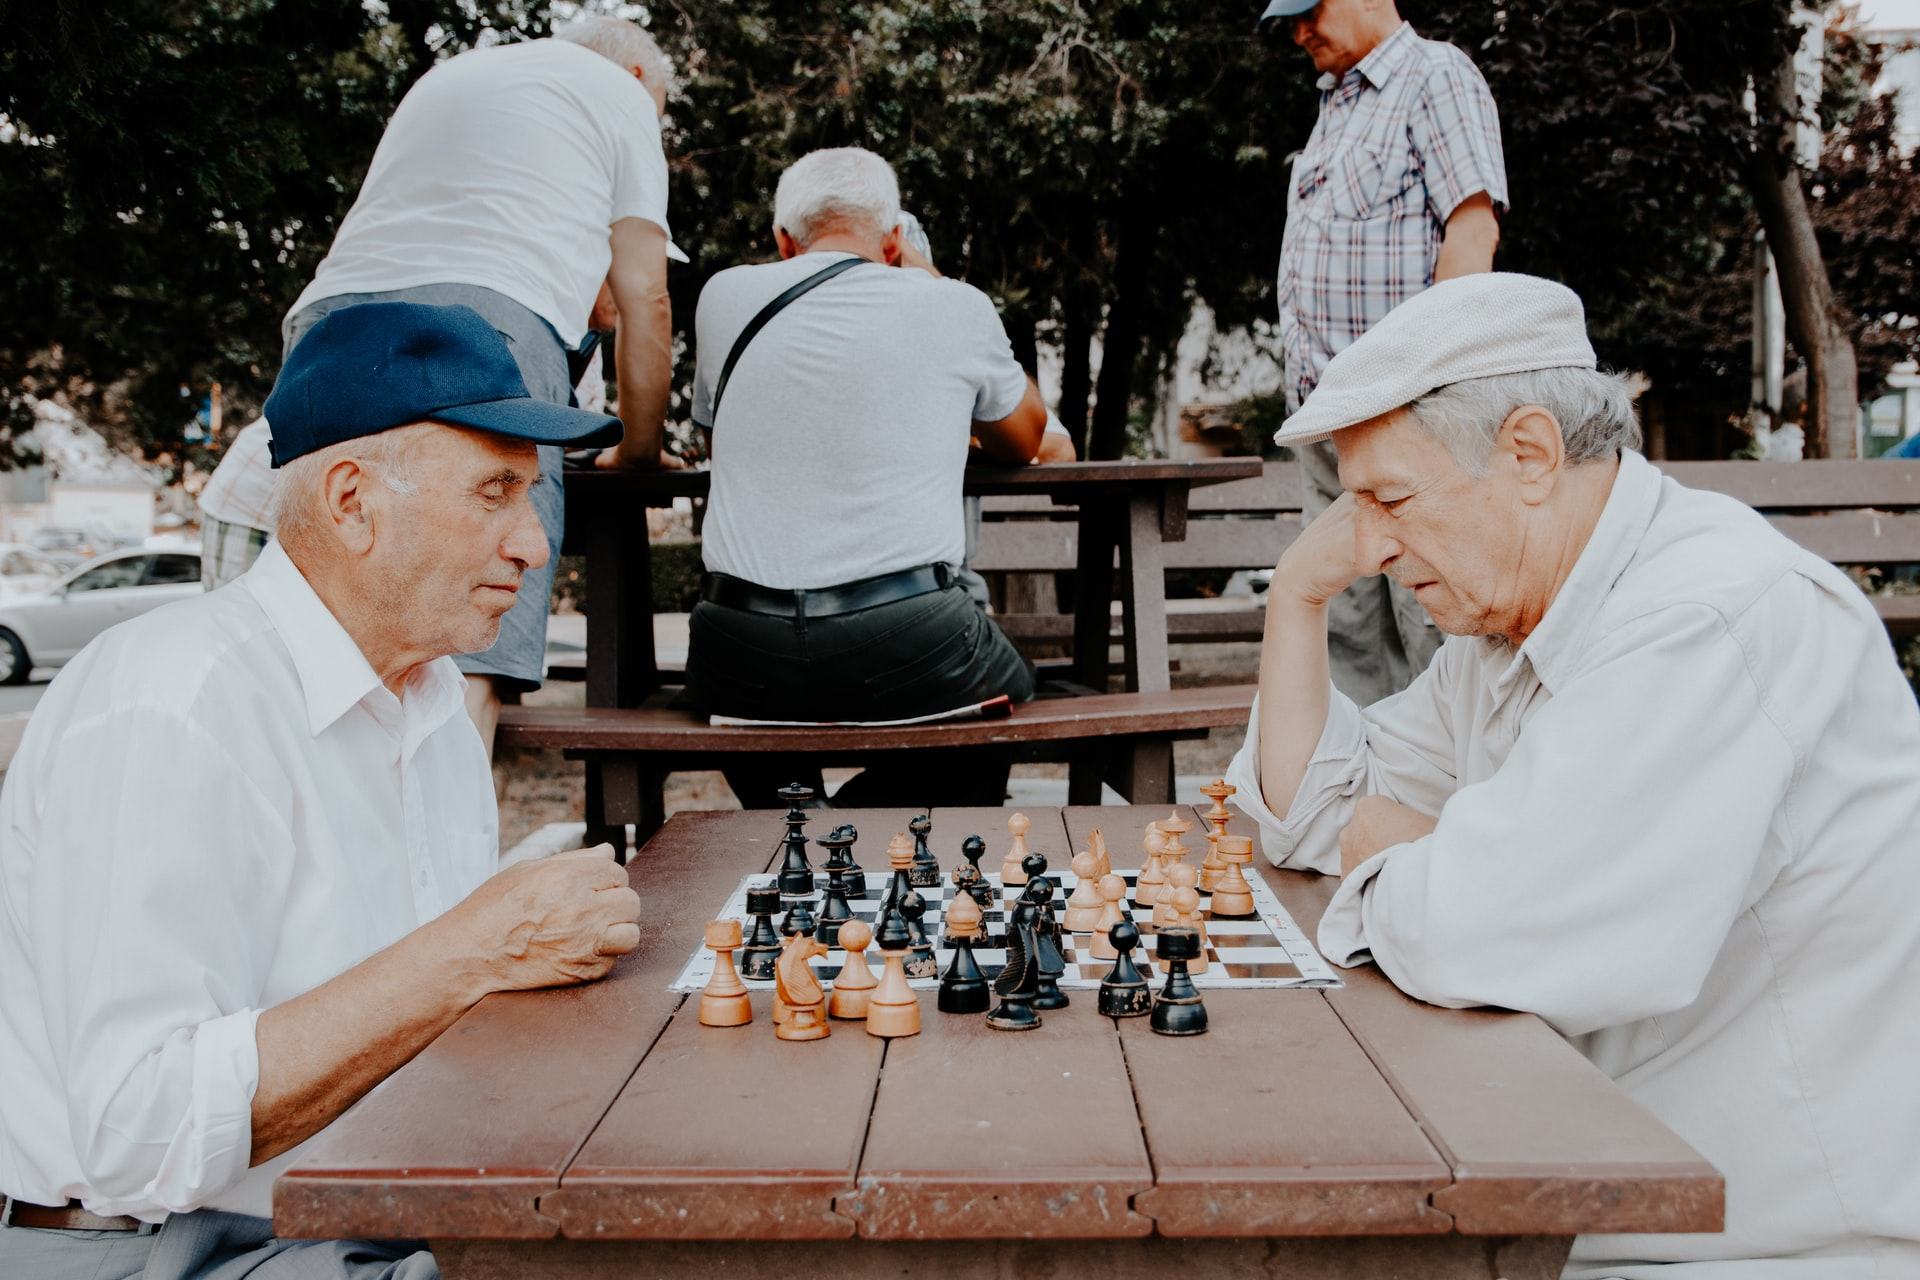
\includegraphics[width=5.5cm]{fig/lec02/chess_elderly_men.jpg}
	\caption{RL in practice (source: Vlad Sargu on \href{https://unsplash.com/photos/ItphH2lGzuI}{Unsplash})}
\end{figure}
}

%%%%%%%%%%%%%%%%%%%%%%%%%%%%%%%%%%%%%%%%%%%%%%%%%%%%%%%%%%%%%
%% Value in MRP %%
%%%%%%%%%%%%%%%%%%%%%%%%%%%%%%%%%%%%%%%%%%%%%%%%%%%%%%%%%%%%%
\frame{\frametitle{Value Function in MRP}
%\vspace{-0.25cm}
\begin{defi}{Value function in MRP}{value_function_MRP}
The \hl{state-value function} $v(x_k)$ of an MRP is the expected return starting from state $x_k$
\begin{equation}
	v(x_k) = \E{G_k|X_k=x_k} .
\end{equation}
\end{defi}
\begin{itemize}
	\item Represents the long-term value of being in state $X_k$.
\end{itemize}
\vspace{0.25cm}
\begin{figure}
	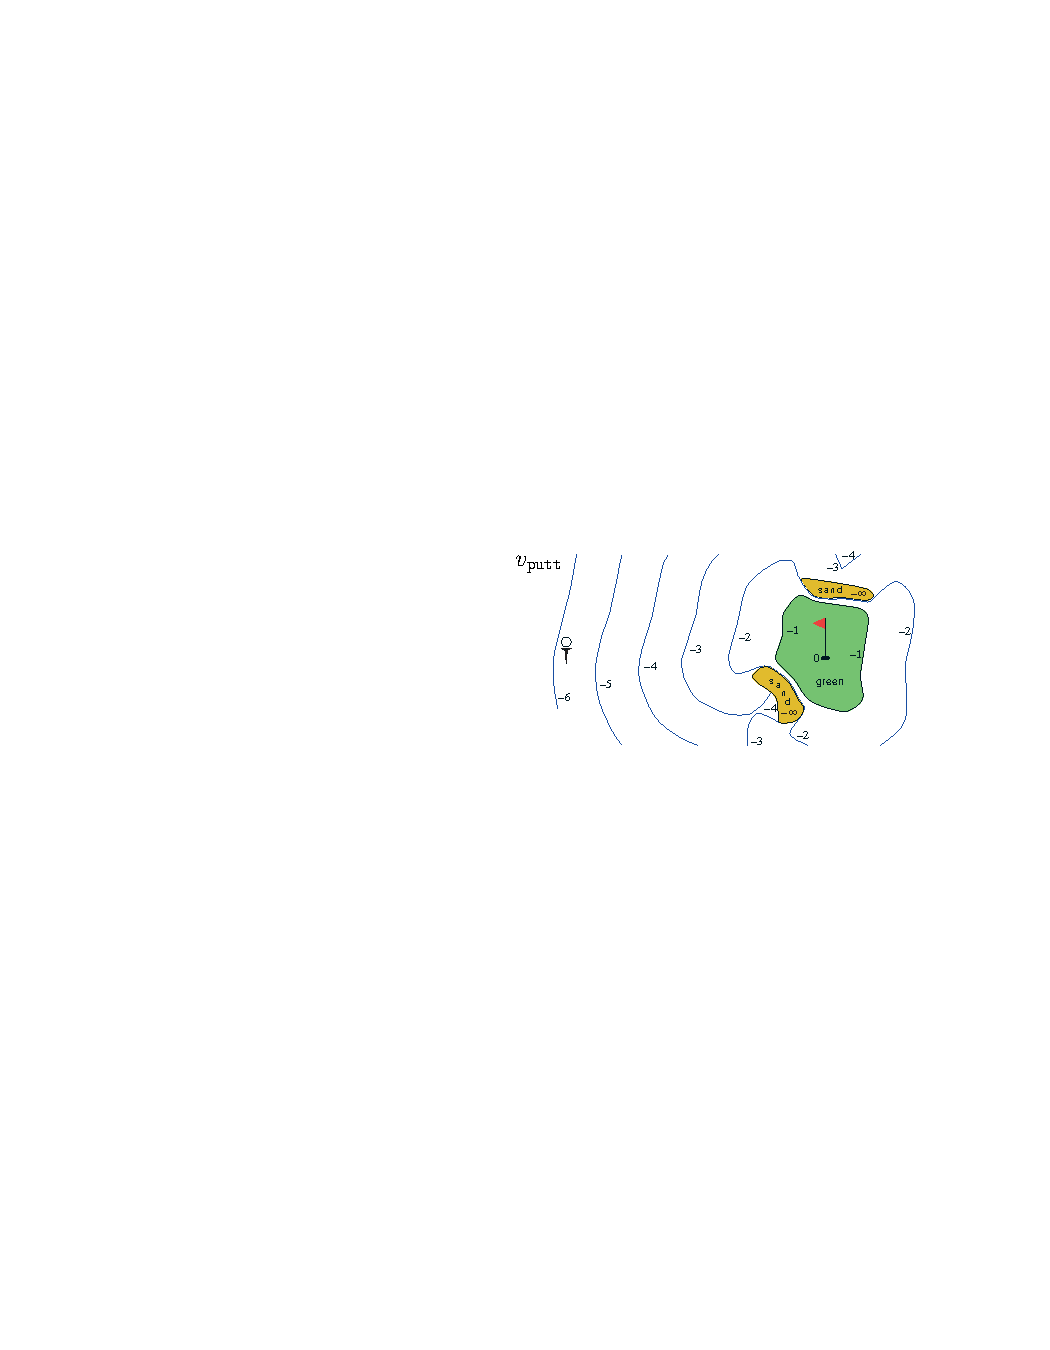
\includegraphics[width=6cm]{fig/lec02/Value_Golf.pdf}
	\caption{Isolines indicate state value of different golf ball locations (source: R. Sutton and G. Barto, Reinforcement learning: an introduction, 2018, \href{https://creativecommons.org/licenses/by-nc-nd/2.0/}{CC BY-NC-ND 2.0})}
	\label{fig:Value_Golf}
\end{figure}
}

%%%%%%%%%%%%%%%%%%%%%%%%%%%%%%%%%%%%%%%%%%%%%%%%%%%%%%%%%%%%%
%% State-Value Samples Forest Markov Reward Process %%
%%%%%%%%%%%%%%%%%%%%%%%%%%%%%%%%%%%%%%%%%%%%%%%%%%%%%%%%%%%%%
\frame{\frametitle{State-Value Samples of Forest MRP}
\begin{figure}		
	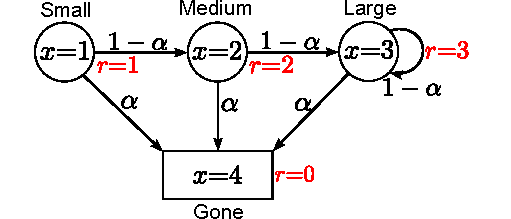
\includegraphics[width=8cm]{fig/lec02/Forest_Markov_Reward_Process.pdf}
\end{figure}
Exemplary \hl{samples} $\hat{v}$ with $\gamma=0.5$ starting in $x=1$:
\begin{alignat*}{2}
	&x=1 \rightarrow 4, &&\hat{v}= 1,\\ 
	&x=1 \rightarrow 2 \rightarrow 4, &&\hat{v}= 1 + 0.5\cdot 2=2.0,\\
	&x=1 \rightarrow 2 \rightarrow 3  \rightarrow 4, \quad&&\hat{v}=1+ 0.5\cdot 2+ 0.25\cdot 3=3.75,\\
	&x=1 \rightarrow 2 \rightarrow 3 \rightarrow 3 \rightarrow 4, \quad&&\hat{v}=1+ 0.5\cdot 2+0.25 \cdot 3+ 0.125\cdot3=4.13.
\end{alignat*}
}

%%%%%%%%%%%%%%%%%%%%%%%%%%%%%%%%%%%%%%%%%%%%%%%%%%%%%%%%%%%%%
%% Bellman Equation for MRPs (1)%%
%%%%%%%%%%%%%%%%%%%%%%%%%%%%%%%%%%%%%%%%%%%%%%%%%%%%%%%%%%%%%
\frame{\frametitle{Bellman Equation for MRPs (1)}
Problem: How to calculate all state values in closed form?\\ 
	\onslide<2->Solution: Bellman equation.
\begin{equation}
\onslide<3->{
\label{eq:Bellman_MRP}
\begin{split}
		v(x_k) &= \E{G_k|X_k=x_k}}\\
							&	\onslide<4->{= \E{R_{k+1} + \gamma R_{k+2} + \gamma^2 R_{k+3}+\ldots|X_k=x_k}}\\
							&\onslide<5->{= \E{R_{k+1} + \gamma \left(R_{k+2} + \gamma R_{k+3}+\ldots\right)|X_k=x_k}}\\
							&\onslide<6->{= \E{R_{k+1} + \gamma G_{k+1}|X_k=x_k}}\\
							&\onslide<7->{= \E{R_{k+1} + \gamma 	v(X_{k+1})|X_k=x_k}}
\end{split}
\end{equation}
\vspace*{\fill}
\onslide<8->{
\begin{figure}	
		 \hspace*{-1.5cm}
		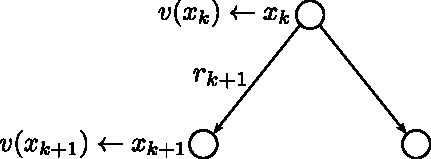
\includegraphics[width=6.1cm]{fig/lec02/Back_Up_MRP.pdf}
		\caption{Backup diagram for $v(x_k)$}
		\label{fig:Back_Up_MRP}
\end{figure}
}
}

%%%%%%%%%%%%%%%%%%%%%%%%%%%%%%%%%%%%%%%%%%%%%%%%%%%%%%%%%%%%%
%% Bellman Equation for MRPs (2) %%
%%%%%%%%%%%%%%%%%%%%%%%%%%%%%%%%%%%%%%%%%%%%%%%%%%%%%%%%%%%%%
\frame{\frametitle{Bellman Equation for MRPs (2)}
Assuming non-random rewards for every state $X=x\in\mathcal{X}$
\begin{equation}
	\bm{r}_{\mathcal{X}}= \begin{bmatrix} \mathcal{R}(x_1) & \cdots & \mathcal{R}(x_n)\end{bmatrix}\T = \begin{bmatrix} \mathcal{R}_1 & \cdots & \mathcal{R}_n\end{bmatrix}\T
\end{equation}
for a finite number of $n$ states with state-values
\begin{equation}
	\bm{v}_{\mathcal{X}}= \begin{bmatrix} v(x_1) & \cdots & v(x_n)\end{bmatrix}\T = \begin{bmatrix} v_1 & \cdots & v_n\end{bmatrix}\T
\end{equation}
one can derive a linear equation system based on \figref{fig:Back_Up_MRP}:\pause
\begin{equation}
\label{eq:Bellman_MRP_linear}
\begin{split}
	\bm{v}_{\mathcal{X}}&=\bm{r}_{\mathcal{X}}+\gamma\bm{\mathcal{P}}_{xx'}\bm{v}_{\mathcal{X}},\\
	\begin{bmatrix} v_1 \\ \vdots \\ v_n \end{bmatrix} &= \begin{bmatrix} \mathcal{R}_1 \\ \vdots \\ \mathcal{R}_n \end{bmatrix} + \gamma\begin{bmatrix} p_{11} & \cdots & p_{1n}\\ \vdots &  & \vdots\\ p_{n1} & \cdots & p_{nn}\end{bmatrix}\begin{bmatrix} v_1 \\ \vdots \\ v_n \end{bmatrix} .
\end{split}
\end{equation}
}

%%%%%%%%%%%%%%%%%%%%%%%%%%%%%%%%%%%%%%%%%%%%%%%%%%%%%%%%%%%%%
%% Sovling the MRP Bellman Equation %%
%%%%%%%%%%%%%%%%%%%%%%%%%%%%%%%%%%%%%%%%%%%%%%%%%%%%%%%%%%%%%
\frame{\frametitle{Solving the MRP Bellman Equation}
Above, \eqref{eq:Bellman_MRP_linear} is a normal equation in $\bm{v}_{\mathcal{X}}$:
\begin{equation}
\label{eq:MRP_normal_equation}
\begin{split}
\bm{v}_{\mathcal{X}}&=\bm{r}_{\mathcal{X}}+\gamma\bm{\mathcal{P}}_{xx'}\bm{v}_{\mathcal{X}},\\
\Leftrightarrow \underbrace{\left(\bm{I}-\gamma\bm{\mathcal{P}}_{xx'}\right)}_{\bm{A}}\underbrace{\bm{v}_{\mathcal{X}}}_{x}&=\underbrace{\bm{r}_{\mathcal{X}}}_{\bm{b}}.
\end{split}
\end{equation}
Possible solutions:
\begin{itemize}
	\item Direct inversion (Gaussian elimination, $\mathcal{O}(n^3)$)\pause
	\item Matrix decomposition (QR, Cholesky, etc. , $\mathcal{O}(n^3)$)\pause
	\item Iterative solutions (e.g., Krylov-subspaces, often better than $\mathcal{O}(n^3)$)\pause
\end{itemize}
\vspace{0.5cm}
In RL identifying and solving \eqref{eq:MRP_normal_equation} is a key task, which is often realized only approximately for high-order state spaces. 
}
%%%%%%%%%%%%%%%%%%%%%%%%%%%%%%%%%%%%%%%%%%%%%%%%%%%%%%%%%%%%%
%% Forest Markov Reward Process with State-Values%%
%%%%%%%%%%%%%%%%%%%%%%%%%%%%%%%%%%%%%%%%%%%%%%%%%%%%%%%%%%%%%
\frame{\frametitle{Example of a Markov Reward Process with State Values}
\begin{figure}		
	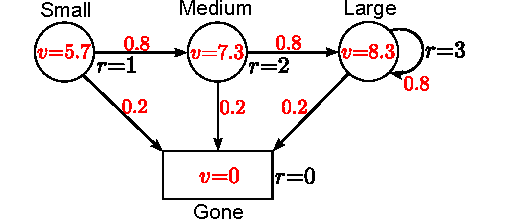
\includegraphics[width=10cm]{fig/lec02/Forest_Markov_Reward_Process_State_Value.pdf}
	\caption{Forest Markov reward process including state values}
	\label{fig:Forest_Markov_Chain_State_Value}
\end{figure}
\begin{itemize}
	\item Discount factor $\gamma=0.8$
	\item Disaster probability $\alpha=0.2$
\end{itemize}
}

%%%%%%%%%%%%%%%%%%%%%%%%%%%%%%%%%%%%%%%%%%%%%%%%%%%%%%%%%%%%%%%%%%
\section{Finite Markov Decision Processes} 
%%%%%%%%%%%%%%%%%%%%%%%%%%%%%%%%%%%%%%%%%%%%%%%%%%%%%%%%%%%%%%%%%%
\begin{frame}
\frametitle{Table of Contents}
\tableofcontents[currentsection]
\end{frame}

%%%%%%%%%%%%%%%%%%%%%%%%%%%%%%%%%%%%%%%%%%%%%%%%%%%%%%%%%%%%%
%% Markov Decision Process %%
%%%%%%%%%%%%%%%%%%%%%%%%%%%%%%%%%%%%%%%%%%%%%%%%%%%%%%%%%%%%%
\frame{\frametitle{Markov Decision Process}

\begin{defi}{Finite Markov decision process}{Markov_decision_process}
A \hl{finite Markov decision process (MDP)} is a tuple $\left\langle\mathcal{X}, \hl{\mathcal{U}}, \bm{\mathcal{P}}, \mathcal{R}, \gamma \right\rangle$ with
\begin{itemize}
	\item $\mathcal{X}$ being a finite set of discrete-time states $X_k\in\mathcal{X}$, 
	\item \hl{$\mathcal{U}$ as a finite set of discrete-time actions $U_k\in\mathcal{U}$,} 
	\item $\bm{\mathcal{P}}=\bm{\mathcal{P}}_{xx'}^{\hl{u}}$ is the state transition probability $\bm{\mathcal{P}}=\Pb{X_{k+1}=x'|X_{k}=x_k, \hl{U_{k}=u_k}}$,
	\item $\mathcal{R}$ is a reward function, $\mathcal{R}=\mathcal{R}_x^{\hl{u}}=\E{R_{k+1}|X_k=x_k, \hl{U_{k}=u_k}}$ and 
	\item $\gamma$ is a discount factor, $\gamma\in\left\{\mathbb{R}|0 \leq \gamma \leq 1\right\}$.
\end{itemize}
\end{defi}
\pause
\begin{itemize}
	\item Markov reward process is extended with actions / decisions.
	\item Now, rewards also depend on action $U_k$.
\end{itemize}
}

%%%%%%%%%%%%%%%%%%%%%%%%%%%%%%%%%%%%%%%%%%%%%%%%%%%%%%%%%%%%%
%% Forest Markov Decision Process (1) %%
%%%%%%%%%%%%%%%%%%%%%%%%%%%%%%%%%%%%%%%%%%%%%%%%%%%%%%%%%%%%%
\frame{\frametitle{Example of a Markov Decision Process (1)}
\begin{figure}		
	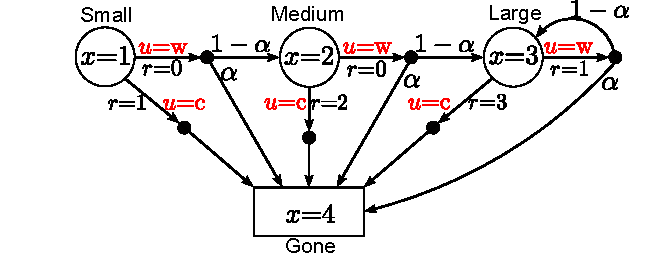
\includegraphics[width=11cm]{fig/lec02/Forest_Markov_Decision_Process.pdf}
	\caption{Forest Markov decision process}
	\label{fig:Forest_Markov_Decision_Process}
\end{figure}

\begin{itemize}
	\item Two actions possible in each state:
	\begin{itemize}
		\item Wait $u=w$: let the tree grow.
		\item Cut $u=c$: gather the wood.
	\end{itemize}
	\item With increasing tree size the wood reward increases as well.
\end{itemize}
}

%%%%%%%%%%%%%%%%%%%%%%%%%%%%%%%%%%%%%%%%%%%%%%%%%%%%%%%%%%%%%
%% Forest Markov Decision Process (2) %%
%%%%%%%%%%%%%%%%%%%%%%%%%%%%%%%%%%%%%%%%%%%%%%%%%%%%%%%%%%%%%
\frame{\frametitle{Example of a Markov Decision Process (2)}
For the previous example the state transition probability matrix and reward function are given as:
\begin{alignat*}{2}
	\bm{\mathcal{P}}_{xx'}^{u=c} &= \begin{bmatrix}0 & 0 & 0 & 1  \\ 0 & 0 &0 & 1 \\ 0 & 0 &0 & 1 \\ 0 & 0 & 0 & 1\end{bmatrix}, \quad \bm{\mathcal{P}}_{xx'}^{u=w} &&= \begin{bmatrix}0 & 1-\alpha & 0 & \alpha  \\ 0 & 0 &1-\alpha & \alpha \\ 0 & 0 &1-\alpha & \alpha \\ 0 & 0 & 0 & 1\end{bmatrix},\\
	\bm{r}_{\mathcal{X}}^{u=c} &= \begin{bmatrix}1 & 2 & 3 & 0 \end{bmatrix}\T, \quad \bm{r}_{\mathcal{X}}^{u=w} &&= \begin{bmatrix}0 & 0 & 1 & 0 \end{bmatrix}\T .
\end{alignat*}
\begin{itemize}
	\item The term $\bm{r}_{\mathcal{X}}^u$ is the abbreviated form for receiving the output of $\mathcal{R}$ for the entire state space $\mathcal{X}$ given the action $u$.
\end{itemize}
}

%%%%%%%%%%%%%%%%%%%%%%%%%%%%%%%%%%%%%%%%%%%%%%%%%%%%%%%%%%%%%
%% Policy (1) %%
%%%%%%%%%%%%%%%%%%%%%%%%%%%%%%%%%%%%%%%%%%%%%%%%%%%%%%%%%%%%%
\frame{\frametitle{Policy (1)}
\onslide<1->{
\begin{defi}{Policy in MDP (1)}{Policy_MDP}
In an MDP environment, a \hl{policy} is a distribution over actions given states:
\begin{equation}
\label{eq:Policy_MDP}
	\pi(u_k|x_k)=\Pb{U_k=u_k  | X_k=x_k}\, .
\end{equation}
\end{defi}
}
\vspace{-0.05cm}
\begin{itemize}
	\onslide<2->{\item In MDP, policies depend only on the current state.}
	\onslide<3->{\item A policy fully defines the agent's behavior.}
	\onslide<4->{\item Might relax to a deterministic policy for certain applications.} 
\end{itemize}
\onslide<1->{
\begin{figure}		
	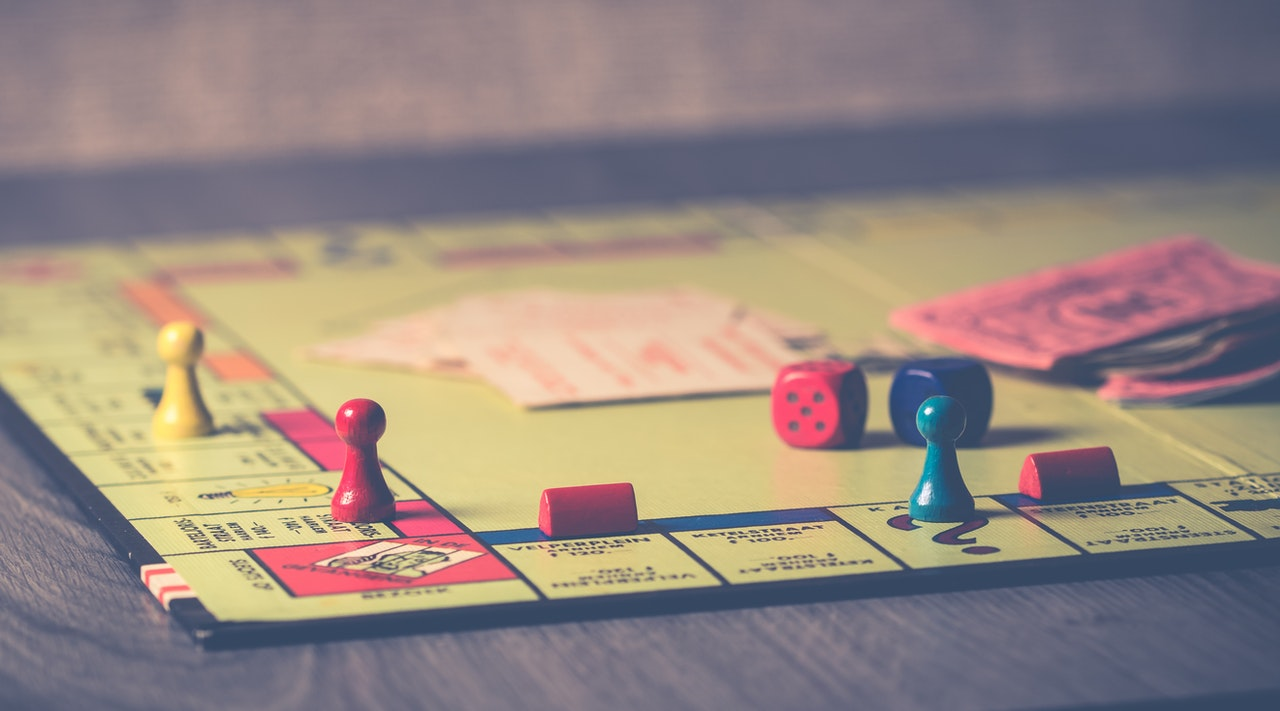
\includegraphics[width=5.75cm]{fig/lec02/monopoly.jpg}
	\caption{What is you best Monopoly policy? (source: Ylanite Koppens on \href{https://www.pexels.com/de-de/foto/begrifflich-brettspiel-drinnen-farben-776654/}{Pexels})}
\end{figure}
}
}

%%%%%%%%%%%%%%%%%%%%%%%%%%%%%%%%%%%%%%%%%%%%%%%%%%%%%%%%%%%%%
%% Policy (2) %%
%%%%%%%%%%%%%%%%%%%%%%%%%%%%%%%%%%%%%%%%%%%%%%%%%%%%%%%%%%%%%
\frame{\frametitle{Policy (2)}
Given an MDP $\left\langle\mathcal{X}, \mathcal{U}, \bm{\mathcal{P}}, \mathcal{R}, \gamma \right\rangle$ and a policy $\bm{\pi}$:
\begin{itemize}
	\item The state sequence $X_k, X_{k+1},\ldots$ is a Markov chain $\left\langle\mathcal{X}, \bm{\mathcal{P}}^{\pi} \right\rangle$ since the state transition probability is only depending on the state:
	\begin{equation}
		\bm{\mathcal{P}}_{xx'}^{\pi}=\sum_{u_k\in\mathcal{U}}\bm{\pi}(u_k|x_k)\bm{\mathcal{P}}_{xx'}^{u}\, .
	\end{equation}\pause
	\item Consequently, the sequence $X_k, R_{k+1}, X_{k+1},R_{k+2},\ldots$ of states and rewards is a Markov reward process $\left\langle\mathcal{X}, \bm{\mathcal{P}}^{\pi}, \mathcal{R}^{\pi}, \gamma \right\rangle$:
	\begin{equation}
		\mathcal{R}_{xx'}^{\pi}=\sum_{u_k\in\mathcal{U}}\bm{\pi}(u_k|x_k)\mathcal{R}_{x}^{u}\, .
	\end{equation}
\end{itemize}
}

%%%%%%%%%%%%%%%%%%%%%%%%%%%%%%%%%%%%%%%%%%%%%%%%%%%%%%%%%%%%%
%% Recap on Value functions %%
%%%%%%%%%%%%%%%%%%%%%%%%%%%%%%%%%%%%%%%%%%%%%%%%%%%%%%%%%%%%%
\frame{\frametitle{Recap on MDP Value Functions}

\begin{defi}{State-value function}{state_value_MDP}
The state-value function of an MDP is the expected return starting in $x_k$ following policy $\pi$:
\begin{equation*}
		v_\pi(x_k) = \El{G_k|X_k=x_k}{\pi}=\El{\left. \sum_{i=0}^\infty \gamma^i R_{k+i+1}\right|X_k}{\pi}\,.
	\end{equation*}
\end{defi}
\pause
\begin{defi}{Action-value function}{action_value_MDP}
The action-value function of an MDP is the expected return starting in $x_k$ taking action $u_k$ following policy $\pi$:
\begin{equation*}
		q_\pi(x_k,u_k) = \El{G_k|X_k=x_k, U_k=u_k}{\pi}=\El{\left.\sum_{i=0}^\infty \gamma^i R_{k+i+1}\right|X_k, U_k}{\pi}\, .
	\end{equation*}
\end{defi}
}

%%%%%%%%%%%%%%%%%%%%%%%%%%%%%%%%%%%%%%%%%%%%%%%%%%%%%%%%%%%%%
%% Bellman Expectation Equation (1) %%
%%%%%%%%%%%%%%%%%%%%%%%%%%%%%%%%%%%%%%%%%%%%%%%%%%%%%%%%%%%%%
\frame{\frametitle{Bellman Expectation Equation (1)}
Analog to \eqref{eq:Bellman_MRP}, the state value of an MDP can be decomposed into a Bellman notation:
\begin{equation}
	v_\pi(x_k)	= \El{R_{k+1} + \gamma 	v_{\pi}(X_{k+1})|X_k=x_k}{\pi}\, .
\end{equation}
\pause
In finite MDPs the state value can be directly linked to the action value (cf.~\figref{fig:Back_Up_Value_MDP}):
\begin{equation}
\label{eq:v_MDP_finite}
	v_\pi(x_k)	= \sum_{u_k\in\mathcal{U}}\pi(u_k|x_k)q_\pi(x_k,u_k) \, .
\end{equation}
\pause
\vspace{0.5cm}
\begin{figure}	
		 \hspace*{-1.5cm}
		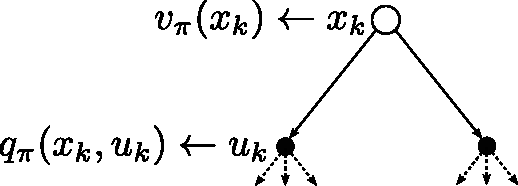
\includegraphics[width=6.5cm]{fig/lec02/Back_Up_Value_MDP.pdf}
		\caption{Backup diagram for $v_{\pi}(x_k)$}
		\label{fig:Back_Up_Value_MDP}
\end{figure}
}

%%%%%%%%%%%%%%%%%%%%%%%%%%%%%%%%%%%%%%%%%%%%%%%%%%%%%%%%%%%%%
%% Bellman Expectation Equation (2) %%
%%%%%%%%%%%%%%%%%%%%%%%%%%%%%%%%%%%%%%%%%%%%%%%%%%%%%%%%%%%%%
\frame{\frametitle{Bellman Expectation Equation (2)}
Likewise, the action value of an MDP can be decomposed into a Bellman notation:
\begin{equation}
	q_\pi(x_k,u_k)	= \El{R_{k+1} + \gamma 	q_{\pi}(X_{k+1},U_{k+1})|X_{k}=x_{k},U_{k}=u_{k}}{\pi}\, .
\end{equation}
\pause
In finite MDPs the action value can be directly linked to the state value (cf.~\figref{fig:Back_Up_Action_Value_MDP}):
\begin{equation}
\label{eq:q_MDP_finite}
	q_\pi(x_k,u_k)	= \mathcal{R}^u_x + \gamma \sum_{x_{k+1}\in\mathcal{X}}p_{xx'}^u v_\pi(x_{k+1}) \, .
\end{equation}
\pause
\vspace{0.5cm}
\begin{figure}	
		 \hspace*{-1.5cm}
		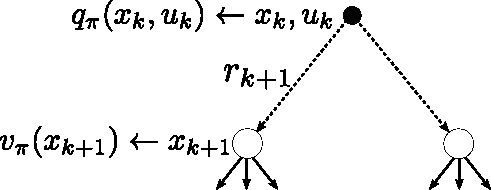
\includegraphics[width=6.5cm]{fig/lec02/Back_Up_Action_Value_MDP.pdf}
		\caption{Backup diagram for $q_{\pi}(x_k,u_k)$}
		\label{fig:Back_Up_Action_Value_MDP}
\end{figure}
}

%%%%%%%%%%%%%%%%%%%%%%%%%%%%%%%%%%%%%%%%%%%%%%%%%%%%%%%%%%%%%
%% Bellman Expectation Equation (3) %%
%%%%%%%%%%%%%%%%%%%%%%%%%%%%%%%%%%%%%%%%%%%%%%%%%%%%%%%%%%%%%
\frame{\frametitle{Bellman Expectation Equation (3)}
Inserting \eqref{eq:q_MDP_finite} into \eqref{eq:v_MDP_finite} directly results in:
\begin{equation}
	v_\pi(x_k)	= \sum_{u_k\in\mathcal{U}}\pi(u_k|x_k)\left(\mathcal{R}^u_x + \gamma\sum_{x_{k+1}\in\mathcal{X}}p_{xx'}^u v_\pi(x_{k+1})\right) \, .
\end{equation}
\pause
Conversely, the action value becomes:
\begin{equation}
	q_\pi(x_k,u_k)	= \mathcal{R}^u_x + \gamma\sum_{x_{k+1}\in\mathcal{X}}p_{xx'}^u \left(\sum_{u_{k+1}\in\mathcal{U}}\pi(u_{k+1}|x_{k+1})q_\pi(x_{k+1},u_{k+1})\right) \, .
\end{equation}
}

%%%%%%%%%%%%%%%%%%%%%%%%%%%%%%%%%%%%%%%%%%%%%%%%%%%%%%%%%%%%%
%% Bellman Expectation Equation in Matrix Form %%
%%%%%%%%%%%%%%%%%%%%%%%%%%%%%%%%%%%%%%%%%%%%%%%%%%%%%%%%%%%%%
\frame{\frametitle{Bellman Expectation Equation in Matrix Form}
Given a policy $\pi$ and following the same assumptions as for \eqref{eq:Bellman_MRP_linear}, the Bellman expectation equation can be expressed in Matrix form:
\begin{equation}
\label{eq:Bellman_MDP_linear}
\begin{split}
	\bm{v}_{\mathcal{X}}^{\pi}&=\bm{r}_{\mathcal{X}}^{\pi}+\gamma\bm{\mathcal{P}}_{xx'}^{\pi}\bm{v}_{\mathcal{X}}^{\pi},\\
	\begin{bmatrix} v_{1}^{\pi} \\ \vdots \\ v_{n}^{\pi} \end{bmatrix} &= \begin{bmatrix} \mathcal{R}_{1}^{\pi} \\ \vdots \\ \mathcal{R}_{n}^{\pi} \end{bmatrix} + \gamma\begin{bmatrix} p_{11}^{\pi} & \cdots & p_{1n}^{\pi}\\ \vdots &  & \vdots\\ p_{n1}^{\pi} & \cdots & p_{nn}^{\pi}\end{bmatrix}\begin{bmatrix} v_{1}^{\pi} \\ \vdots \\ v_{n}^{\pi} \end{bmatrix}.
\end{split}
\end{equation}
Here, $\bm{r}_{\mathcal{X}}^{\pi}$ and $\bm{\mathcal{P}}_{xx'}^{\pi}$ are the rewards and state transition probability following policy $\pi$. \pause Hence, the state value can be calculated by solving \eqref{eq:Bellman_MDP_linear} for $\bm{v}_{\mathcal{X}}^{\pi}$, e.g., by direct matrix inversion:
\begin{equation}
	\bm{v}_{\mathcal{X}}^{\pi}=\left(\bm{I}-\gamma\bm{\mathcal{P}}_{xx'}^{\pi}\right)^{-1}\bm{r}_{\mathcal{X}}^{\pi}.
\end{equation}
}

%%%%%%%%%%%%%%%%%%%%%%%%%%%%%%%%%%%%%%%%%%%%%%%%%%%%%%%%%%%%%
%% Bellman Expectation Equation Applied to Forest Tree Example (1)%%
%%%%%%%%%%%%%%%%%%%%%%%%%%%%%%%%%%%%%%%%%%%%%%%%%%%%%%%%%%%%%
\frame{\frametitle{Bellman Expectation Equation \& Forest Tree Example (1)}
Let's assume following very simple policy ('\textit{fifty-fifty}')
\begin{equation*}
\pi(u = \mbox{cut}|x) = 0.5, \quad \pi(u = \mbox{wait}|x) = 0.5 \quad\forall x\in\mathcal{X} \, .
\end{equation*}
\pause
Applied to the given environment behavior
\begin{alignat*}{2}
	\bm{\mathcal{P}}_{xx'}^{u=c} &= \begin{bmatrix}0 & 0 & 0 & 1  \\ 0 & 0 &0 & 1 \\ 0 & 0 &0 & 1 \\ 0 & 0 & 0 & 1\end{bmatrix}, \quad \bm{\mathcal{P}}_{xx'}^{u=w} &&= \begin{bmatrix}0 & 1-\alpha & 0 & \alpha  \\ 0 & 0 &1-\alpha & \alpha \\ 0 & 0 &1-\alpha & \alpha \\ 0 & 0 & 0 & 1\end{bmatrix},\\
	\bm{r}_{\mathcal{X}}^{u=c} &= \begin{bmatrix}1 & 2 & 3 & 0 \end{bmatrix}\T, \quad \bm{r}_{\mathcal{X}}^{u=w} &&= \begin{bmatrix}0 & 0 & 1 & 0 \end{bmatrix}\T ,
\end{alignat*}
\pause
one receives:
\begin{equation*}
	\bm{\mathcal{P}}_{xx'}^{\pi} = \begin{bmatrix}0 & \frac{1-\alpha}{2} & 0 & \frac{1+\alpha}{2}  \\ 0 & 0 &\frac{1-\alpha}{2} & \frac{1+\alpha}{2} \\ 0 & 0 &\frac{1-\alpha}{2} & \frac{1+\alpha}{2} \\ 0 & 0 & 0 & 1\end{bmatrix}, \quad\bm{r}_{\mathcal{X}}^{\pi} = \begin{bmatrix}0.5 \\ 1 \\ 2 \\ 0 \end{bmatrix} .
\end{equation*}
}

%%%%%%%%%%%%%%%%%%%%%%%%%%%%%%%%%%%%%%%%%%%%%%%%%%%%%%%%%%%%%
%% Bellman Expectation Equation Applied to Forest Tree Example (2)%%
%%%%%%%%%%%%%%%%%%%%%%%%%%%%%%%%%%%%%%%%%%%%%%%%%%%%%%%%%%%%%
\frame{\frametitle{Bellman Expectation Equation \& Forest Tree Example (2)}
\begin{figure}		
	%\hspace*{-1.5cm}
	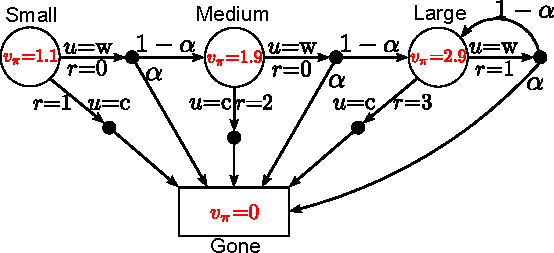
\includegraphics[width=10cm]{fig/lec02/Forest_Markov_Decision_Process_State_Value.pdf}
	\caption{Forest MDP with fifty-fifty-policy including state values}
	\label{fig:Forest_Markov_Decision_Process_State_Value}
\end{figure}
\begin{itemize}
	\item Discount factor $\gamma=0.8$
	\item Disaster probability $\alpha=0.2$
\end{itemize}
}

%%%%%%%%%%%%%%%%%%%%%%%%%%%%%%%%%%%%%%%%%%%%%%%%%%%%%%%%%%%%%
%% Bellman Expectation Equation Applied to Forest Tree Example (3)%%
%%%%%%%%%%%%%%%%%%%%%%%%%%%%%%%%%%%%%%%%%%%%%%%%%%%%%%%%%%%%%
\frame{\frametitle{Bellman Expectation Equation \& Forest Tree Example (3)}
Using the Bellman expectation eq. \eqref{eq:q_MDP_finite} the action values can be directly calculated: 
\vspace{0.5cm}
\begin{figure}		
	\hspace*{0.5cm}
	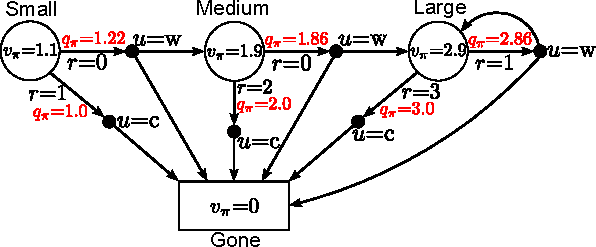
\includegraphics[width=10cm]{fig/lec02/Forest_Markov_Decision_Process_Action_Value.pdf}
	\caption{Forest MDP with fifty-fifty-policy plus action values}
	\label{fig:Forest_Markov_Decision_Process_Action_Value}
\end{figure}
Is the '\textit{fifty-fifty-policy}' maximizing our long-term reward? How can you evaluate your answer?
}

%%%%%%%%%%%%%%%%%%%%%%%%%%%%%%%%%%%%%%%%%%%%%%%%%%%%%%%%%%%%%%%%%%
\section{Optimal Policies and Value Functions} 
%%%%%%%%%%%%%%%%%%%%%%%%%%%%%%%%%%%%%%%%%%%%%%%%%%%%%%%%%%%%%%%%%%
\begin{frame}
\frametitle{Table of Contents}
\tableofcontents[currentsection]
\end{frame}

%%%%%%%%%%%%%%%%%%%%%%%%%%%%%%%%%%%%%%%%%%%%%%%%%%%%%%%%%%%%%
%% Optimal Value Functions in MDP %%
%%%%%%%%%%%%%%%%%%%%%%%%%%%%%%%%%%%%%%%%%%%%%%%%%%%%%%%%%%%%%
\frame{\frametitle{Optimal Value Functions in an MDP}
\begin{defi}{Optimal state-value function}{optimal_state_value_MDP}
The optimal state-value function of an MDP is the maximum state-value function over all polices:
\begin{equation}
		v^*(x) = \max_{\pi} v_{\pi}(x)\,.
	\end{equation}
\end{defi}
\vspace{-0.2cm}
\pause
\begin{defi}{Optimal action-value function}{optimal_action_value_MDP}
The optimal action-value function of an MDP is the maximum action-value function over all polices:
\begin{equation}
		q^*(x,u) = \max_{\pi} q_\pi(x,u)\, .
	\end{equation}
\end{defi}
\vspace{-0.1cm}
\pause
\begin{itemize}
	\item The optimal value function denotes the best possible agent's performance for a given MDP / environment. \pause
	\item A (finite) MDP can be easily solved in an optimal way if $q^*(x,u)$ is known. 
\end{itemize}
}

%%%%%%%%%%%%%%%%%%%%%%%%%%%%%%%%%%%%%%%%%%%%%%%%%%%%%%%%%%%%%
%% Optimal Policy in MDP %%
%%%%%%%%%%%%%%%%%%%%%%%%%%%%%%%%%%%%%%%%%%%%%%%%%%%%%%%%%%%%%
\frame{\frametitle{Optimal Policy in an MDP}
Define a partial ordering over polices
\begin{equation}
	\pi \geq \pi' \quad \mbox{if} \quad v_{\pi}(x) \geq v_{\pi'}(x) \quad \forall x\in\mathcal{X} \,.
\end{equation}
\pause
\begin{theo}{Optimal policies in MDPs}{Optimal_policies_MDP}
For any finite MDP
\begin{itemize}
	\item there exists an optimal policy $\pi^*\geq\pi$ that is better or equal to all other policies,
	\item all optimal policies achieve the same optimal state-value function $v^*(x)=v_{\pi^*}(x)$,
	\item all optimal policies achieve the same optimal action-value function $q^*(x, u)=q_{\pi^*}(x, u)$.
\end{itemize}
\end{theo}
}

%%%%%%%%%%%%%%%%%%%%%%%%%%%%%%%%%%%%%%%%%%%%%%%%%%%%%%%%%%%%%
%% Bellman Optimality Equation (1)%%
%%%%%%%%%%%%%%%%%%%%%%%%%%%%%%%%%%%%%%%%%%%%%%%%%%%%%%%%%%%%%
\frame{\frametitle{Bellman Optimality Equation (1)}
\onslide<1->{
\begin{theo}{Bellman's principle of optimality}{bellman_principle_optimality}
``\textit{An optimal policy has the property that whatever the initial state and initial decision are, the remaining decisions must constitute an optimal policy with regard to the state resulting from the first decision.}''(R.E. Bellman, Dynamic Programming, 1957) 
\end{theo}
}
\begin{itemize}
	\onslide<2->{\item Any policy (i.e., also the optimal one) must satisfy the self-consistency condition given by the Bellman expectation equation.}
	\onslide<3->{\item An optimal policy must deliver the maximum expected return being in a given state:}
\end{itemize}
\onslide<4->{
\begin{equation}
\begin{split}
		v^*(x_k) &= \max_{u} q_{\pi^*}(x_k, u)\, ,}\\
									&\onslide<5->{= \max_{u} \El{G_k|X_k=x_k, U=u}{\pi^*}\, ,}\\
									&\onslide<6->{= \max_{u} \El{R_{k+1} + \gamma G_{k+1}|X_k=x_k, U=u}{\pi^*}\, ,}\\
									&\onslide<7->{= \max_{u} \E{R_{k+1} + \gamma v^*(X_{k+1})|X_k=x_k, U=u}\, .}
\end{split}
\end{equation}
}

%%%%%%%%%%%%%%%%%%%%%%%%%%%%%%%%%%%%%%%%%%%%%%%%%%%%%%%%%%%%%
%% Bellman Optimality Equation (2)%%
%%%%%%%%%%%%%%%%%%%%%%%%%%%%%%%%%%%%%%%%%%%%%%%%%%%%%%%%%%%%%
\frame{\frametitle{Bellman Optimality Equation (2)}
Again, the Bellman optimality equation can be visualized by a backup diagram: 
\begin{figure}	
		 %\hspace*{-1.5cm}
		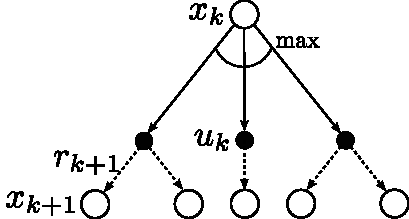
\includegraphics[width=4.5cm]{fig/lec02/Back_Up_Value_Optimal_MDP.pdf}
		\caption{Backup diagram for $v^*(x_k)$}
		\label{fig:Back_Up_Value_Optimal_MDP}
\end{figure}
\pause
For a finite MDP the following expression results:
\begin{equation}
\label{eq:Bellman_Optimal_State_Value_MDP}
	v^*(x_k) = \max_{u_k}\, \mathcal{R}^u_x+ \gamma \sum_{x_{k+1}\in\mathcal{X}}p_{xx'}^u v_{\pi^*}(x_{k+1}) .
\end{equation}
}

%%%%%%%%%%%%%%%%%%%%%%%%%%%%%%%%%%%%%%%%%%%%%%%%%%%%%%%%%%%%%
%% Bellman Optimality Equation (3)%%
%%%%%%%%%%%%%%%%%%%%%%%%%%%%%%%%%%%%%%%%%%%%%%%%%%%%%%%%%%%%%
\frame{\frametitle{Bellman Optimality Equation (3)}
Likewise, the Bellman optimality equation is applicable to the action value:
\begin{equation}
	q^*(x_k,u_k) = \E{R_{k+1}+ \gamma \max_{u_{k+1}} q^*(X_{k+1},U_{k+1})|X_k=x_k, U_k=u_k} . 
\end{equation}
\pause
And, in the finite MDP case:
\begin{equation}
\label{eq:Bellman_Optimal_action_Value_MDP}
	q^*(x_k,u_k) = \mathcal{R}^u_x + \gamma \sum_{x_{k+1}\in\mathcal{X}}p_{xx'}^u \max_{u_{k+1}}q^*(x_{k+1}, u_{k+1}) .
\end{equation}
\pause
\begin{figure}	
		 %\hspace*{-1.5cm}
		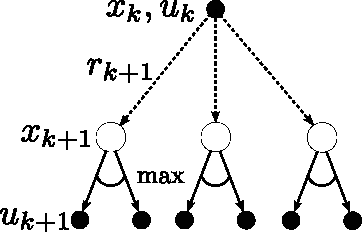
\includegraphics[width=4.7cm]{fig/lec02/Back_Up_Action_Value_Optimal_MDP.pdf}
		\caption{Backup diagram for $q^*(x_k,u_k)$}
		\label{fig:Back_Up_Action_Value_Optimal_MDP}
\end{figure}
}

%%%%%%%%%%%%%%%%%%%%%%%%%%%%%%%%%%%%%%%%%%%%%%%%%%%%%%%%%%%%%
%% Solving the Bellman Optimality Equation %%
%%%%%%%%%%%%%%%%%%%%%%%%%%%%%%%%%%%%%%%%%%%%%%%%%%%%%%%%%%%%%
\frame{\frametitle{Solving the Bellman Optimality Equation}
\begin{itemize}
	\item In finite MDPs with $n$ states, \eqref{eq:Bellman_Optimal_State_Value_MDP} delivers an \hl{algebraic equation system} with $n$ unknowns and $n$ \hl{state-value equations}. \pause
	\item Likewise, \eqref{eq:Bellman_Optimal_action_Value_MDP} delivers an algebraic equation system with up to $n\cdot m$ unknowns and $n \cdot m$ \hl{action-value equations} ($m=$number of actions). \pause
	\item Due to $\max$ operator the equation set is generally \hl{nonlinear}. Direct, closed form solution rarely available. \pause
	\item Hence, often  approximate / iterative solutions are required (upcoming lectures).\pause
	\item If environment is exactly known, solving for $v^*$ or $q^*$ directly delivers optimal policy. 
	\begin{itemize}
		\item If $v(x)$ is known, a one-step-ahead search is required to get $q(x)$.
		\item If $q(x, u)$ is known, directly choose $q^*$. \pause
	\end{itemize}
	\item Even though above decisions are very short sighted (one-step-ahead search for $v$ or direct choice of $q$), by Bellman's principle of optimality one receives the long-term maximum of the expected reward.
\end{itemize}
}

%%%%%%%%%%%%%%%%%%%%%%%%%%%%%%%%%%%%%%%%%%%%%%%%%%%%%%%%%%%%%
%% Optimal Forest MDP %%
%%%%%%%%%%%%%%%%%%%%%%%%%%%%%%%%%%%%%%%%%%%%%%%%%%%%%%%%%%%%%
\frame{\frametitle{Optimal Policy for Forest Tree MDP}
Remember the forest tree MDP example:
\begin{figure}		
	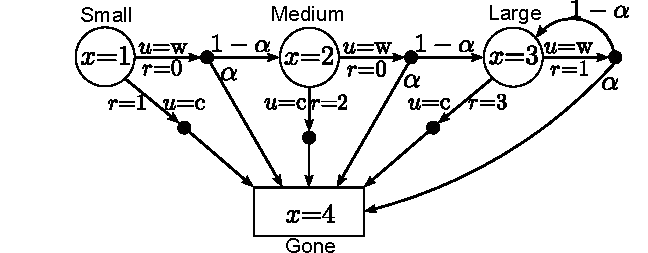
\includegraphics[width=11cm]{fig/lec02/Forest_Markov_Decision_Process_No_Color.pdf}
	\label{fig:Forest_Markov_Decision_Process_No_Color}
\end{figure}

\begin{itemize}
	\item Two actions possible in each state:
	\begin{itemize}
		\item Wait $u=w$: let the tree grow.
		\item Cut $u=c$: gather the wood.
	\end{itemize}
	\item Lets first calculate $v^*(x)$ and then $q^*(x,u)$.
\end{itemize}
}

%%%%%%%%%%%%%%%%%%%%%%%%%%%%%%%%%%%%%%%%%%%%%%%%%%%%%%%%%%%%%
%% Optimal Policy for Forest Tree MDP: State-Value (1)%%
%%%%%%%%%%%%%%%%%%%%%%%%%%%%%%%%%%%%%%%%%%%%%%%%%%%%%%%%%%%%%
\frame{\frametitle{Optimal Policy for Forest Tree MDP: State Value (1)}
\onslide<1->{Start with $v(x=4)$ ('gone') and then continue going backwards:}
\onslide<2->{
\begin{align*}
	v^*(x=4) &= 0\, ,}\\
	\onslide<3->{v^*(x=3) &= \max \begin{cases} 1 + \gamma\left[(1-\alpha)v^*(x=3) + \alpha v^*(x=4)\right]\, ,\\ 3+\gamma v^*(x=4)\, ,\end{cases}}\\
					 &\onslide<4->{= \max \begin{cases} 1 + \gamma\left[(1-\alpha)v^*(x=3)\right]\, ,\\ 3\, ,\end{cases}}\\\
	\onslide<5->{v^*(x=2) &= \max \begin{cases} 0 + \gamma\left[(1-\alpha)v^*(x=3) + \alpha v^*(x=4)\right]\, ,\\ 2+\gamma v^*(x=4)\, ,\end{cases}}\\
					 &\onslide<6->{= \max \begin{cases} \gamma\left[(1-\alpha)v^*(x=3)\right]\, ,\\ 2\, ,\end{cases}}\\
	\onslide<7->{v^*(x=1) &= \max \begin{cases} \gamma\left[(1-\alpha)v^*(x=2)\right]\, ,\\ 1\, .\end{cases}}
\end{align*}
}

%%%%%%%%%%%%%%%%%%%%%%%%%%%%%%%%%%%%%%%%%%%%%%%%%%%%%%%%%%%%%
%% Optimal Policy for Forest Tree MDP: State-Value (2)%%
%%%%%%%%%%%%%%%%%%%%%%%%%%%%%%%%%%%%%%%%%%%%%%%%%%%%%%%%%%%%%
\frame{\frametitle{Optimal Policy for Forest Tree MDP: State Value (2)}
\begin{itemize}
	\item Due to presence of terminal state ($x=4$) only three unknowns
	\item Solution: numerical optimization approach (e.g., simplex method, gradient descent,...)
\end{itemize}
\begin{figure}		
	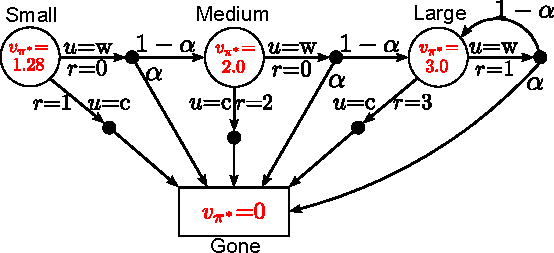
\includegraphics[width=11cm]{fig/lec02/Forest_Markov_Decision_Process_Optimal_State_Value.pdf}
		\caption{State values under optimal policy ($\gamma=0.8$,	$\alpha=0.2$)}
	\label{fig:Forest_Markov_Decision_Process_Optimal_State_Value}
\end{figure}
}

%%%%%%%%%%%%%%%%%%%%%%%%%%%%%%%%%%%%%%%%%%%%%%%%%%%%%%%%%%%%%
%% Optimal Policy for Forest Tree MDP: State-Value (3)%%
%%%%%%%%%%%%%%%%%%%%%%%%%%%%%%%%%%%%%%%%%%%%%%%%%%%%%%%%%%%%%
\frame{\frametitle{Optimal Policy for Forest Tree MDP: State Value (3)}
\begin{figure}		
	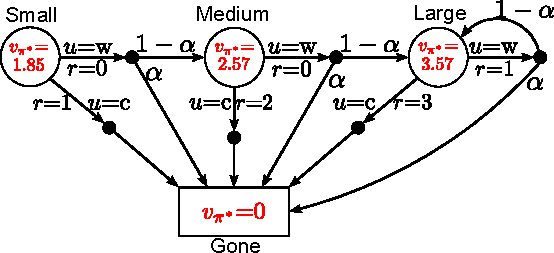
\includegraphics[width=11cm]{fig/lec02/Forest_Markov_Decision_Process_Optimal_State_Value_Gamma09.pdf}
		\caption{State values under optimal policy (\hl{$\gamma=0.9$},	$\alpha=0.2$)}
	\label{fig:Forest_Markov_Decision_Process_Optimal_State_Value_Gamma09}
\end{figure}
}

%%%%%%%%%%%%%%%%%%%%%%%%%%%%%%%%%%%%%%%%%%%%%%%%%%%%%%%%%%%%%
%% Optimal Policy for Forest Tree MDP: Action-Value (1)%%
%%%%%%%%%%%%%%%%%%%%%%%%%%%%%%%%%%%%%%%%%%%%%%%%%%%%%%%%%%%%%
\frame{\frametitle{Optimal Policy for Forest Tree MDP: Action Value (1)}
\onslide<1->{Use $u_{k+1}=u'$ to set up equation system:
\begin{align*}
q^*(x=1,u=c) &= 1\, ,}\\
\onslide<2->{q^*(x=1,u=w) &= \gamma(1-\alpha)\max_{u'}q^*(x=2,u')\, ,}\\
\onslide<3->{q^*(x=2,u=c) &= 2\, ,}\\
\onslide<4->{q^*(x=2,u=w) &= \gamma(1-\alpha)\max_{u'}q^*(x=3,u')\, ,}\\
\onslide<5->{q^*(x=3,u=c) &= 3\, ,}\\
\onslide<6->{q^*(x=3,u=w) &= 1+\gamma(1-\alpha)\max_{u'}q^*(x=3,u')\, .}
\end{align*}
\onslide<7->{
\begin{itemize}
	\item There are six action-state pairs in total.
	\item Three of them can be directly determined.
	\item Three unknowns and three equations remain.
\end{itemize}
}
}

%%%%%%%%%%%%%%%%%%%%%%%%%%%%%%%%%%%%%%%%%%%%%%%%%%%%%%%%%%%%%
%% Optimal Policy for Forest Tree MDP: Action-Value (2)%%
%%%%%%%%%%%%%%%%%%%%%%%%%%%%%%%%%%%%%%%%%%%%%%%%%%%%%%%%%%%%%
\frame{\frametitle{Optimal Policy for Forest Tree MDP: Action Value (2)}
\onslide<1->{
Rearrange $\max$ expressions for unknown action values: 
\begin{align*}
q^*(x=1,u=w) &= \gamma(1-\alpha)\max\begin{cases}\gamma(1-\alpha)\max\begin{cases}1+\gamma(1-\alpha)q^*(3,w)\\3\end{cases}\\2\end{cases}}\\
\onslide<2->{q^*(x=2,u=w) &= \gamma(1-\alpha)\max\begin{cases}1+\gamma(1-\alpha)q^*(3,w)\\3\end{cases}}\\
\onslide<3->{q^*(x=3,u=w) &= 1+\gamma(1-\alpha)\max\begin{cases}q^*(3,w)\\3\end{cases}\, .}
\end{align*}
\onslide<4->{Again, retrieve unknown optimal action values by numerical optimization solvers.}
}

%%%%%%%%%%%%%%%%%%%%%%%%%%%%%%%%%%%%%%%%%%%%%%%%%%%%%%%%%%%%%
%% Optimal Policy for Forest Tree MDP: Action-Value (3)%%
%%%%%%%%%%%%%%%%%%%%%%%%%%%%%%%%%%%%%%%%%%%%%%%%%%%%%%%%%%%%%
\frame{\frametitle{Optimal Policy for Forest Tree MDP: Action Value (3)}
\begin{figure}		
	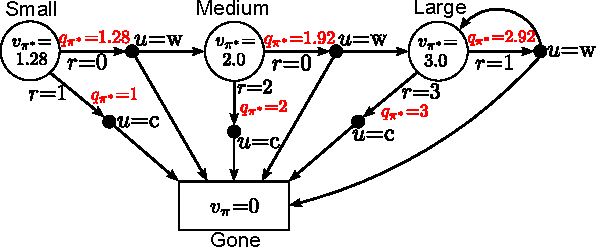
\includegraphics[width=11cm]{fig/lec02/Forest_Markov_Decision_Process_Optimal_Action_Value.pdf}
		\caption{Action values under optimal policy ($\gamma=0.8$,	$\alpha=0.2$)}
	\label{fig:Forest_Markov_Decision_Process_Optimal_Action_Value}
\end{figure}
}

%%%%%%%%%%%%%%%%%%%%%%%%%%%%%%%%%%%%%%%%%%%%%%%%%%%%%%%%%%%%%
%% Optimal Policy for Forest Tree MDP: Action-Value (4)%%
%%%%%%%%%%%%%%%%%%%%%%%%%%%%%%%%%%%%%%%%%%%%%%%%%%%%%%%%%%%%%
\frame{\frametitle{Optimal Policy for Forest Tree MDP: Action Value (4)}
\begin{figure}		
	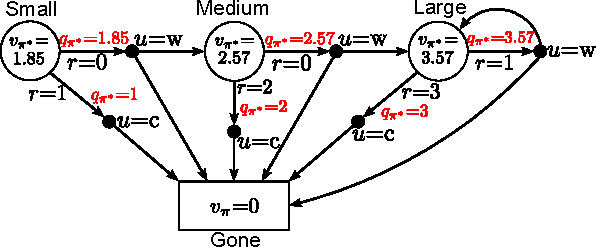
\includegraphics[width=11cm]{fig/lec02/Forest_Markov_Decision_Process_Optimal_Action_Value_Gamma09.pdf}
		\caption{Action values under optimal policy (\hl{$\gamma=0.9$},	$\alpha=0.2$)}
	\label{fig:Forest_Markov_Decision_Process_Optimal_Action_Value_Gamma09}
\end{figure}
}

%%%%%%%%%%%%%%%%%%%%%%%%%%%%%%%%%%%%%%%%%%%%%%%%%%%%%%%%%%%%%
%% Solving an MDP by Calculating Optimal State and Action-Values%%
%%%%%%%%%%%%%%%%%%%%%%%%%%%%%%%%%%%%%%%%%%%%%%%%%%%%%%%%%%%%%
\frame{\frametitle{Direct Numerical State and Action-Value Calculation}
\begin{itemize}
	\item Possible only for \hl{small action and state-space} MDPs
	\begin{itemize}
		\item 'Solving' Backgammon with $\approx 10^{20}$ states?
	\end{itemize}
	\pause
	\item Another issue: initial values?\pause
	\item And yet another issue: \hl{nonlinear system with multiple unknowns}
		\begin{itemize}
			\item Local solvers = local solutions
			\item Initial-point-dependent 
		\end{itemize}
		\pause
		\item And finally: total \hl{environment knowledge} required
\end{itemize}
\pause
\begin{block}{Framing the reinforcement learning problem}
Facing the above issues, RL addresses mainly two topics:
\begin{itemize}
	\item Approximate solutions of complex decision problems.
	\item Learning of such approximations based on environment interactions.
\end{itemize}
 
\end{block}
}

%%%%%%%%%%%%%%%%%%%%%%%%%%%%%%%%%%%%%%%%%%%%%%%%%%%%%%%%%%%%%
%% Summary %%
%%%%%%%%%%%%%%%%%%%%%%%%%%%%%%%%%%%%%%%%%%%%%%%%%%%%%%%%%%%%%
\begin{frame}
\frametitle{Summary: What You've Learned Today}
\begin{itemize}
	\item Differentiate finite Markov process models with or w/o rewards and actions.\pause
	\item Interpret such stochastic processes as simplified abstractions of real-world problems.\pause
	\item Understand the importance of value functions to describe the agent's performance. \pause
	\item Formulate value-function equation systems by the Bellman principle.\pause
	\item Recognize optimal policies.\pause
	\item Setting up nonlinear equation systems for retrieving optimal policies by the Bellman principle.\pause
	\item Solving for different value functions in MRP/MDP contexts by numerical optimization.
\end{itemize}
\end{frame}

\part{Lecture 03: Dynamic Programming}
\title[RL Lecture 03]{Lecture 03: Dynamic Programming}  
\date{}  
\frame{\titlepage} 
\frame{\frametitle{Table of contents}\tableofcontents} 

%%%%%%%%%%%%%%%%%%%%%%%%%%%%%%%%%%%%%%%%%%%%%%%%%%%%%%%%%%%%%%%%%%
\section{Introduction} 
%%%%%%%%%%%%%%%%%%%%%%%%%%%%%%%%%%%%%%%%%%%%%%%%%%%%%%%%%%%%%%%%%%

%%%%%%%%%%%%%%%%%%%%%%%%%%%%%%%%%%%%%%%%%%%%%%%%%%%%%%%%%%%%%
%% What is Dynamic Programming? %%
%%%%%%%%%%%%%%%%%%%%%%%%%%%%%%%%%%%%%%%%%%%%%%%%%%%%%%%%%%%%%
\frame{\frametitle{what is dynamic programming (dp)?}

\begin{block}{Basic DP definition}
\begin{itemize}
	\item \hl{Dynamic}: sequential or temporal problem structure
	\item \hl{Programming}: mathematical optimization, i.e., numerical solutions
\end{itemize}
\end{block}
\pause
\vspace{1cm}
Further characteristics:
\begin{itemize}
	\item DP is a collection of algorithms to solve MDPs and neighboring problems.
	\begin{itemize}
		\item \hl{We will focus only on finite MDPs.}
		\item In case of continuous action/state space: apply quantization.
	\end{itemize}\pause
	\item Use of value functions to organize and structure the search for an optimal policy.
	\item Breaks problems into subproblems and solves them.
\end{itemize}
}

%%%%%%%%%%%%%%%%%%%%%%%%%%%%%%%%%%%%%%%%%%%%%%%%%%%%%%%%%%%%%
%% Requirements %%
%%%%%%%%%%%%%%%%%%%%%%%%%%%%%%%%%%%%%%%%%%%%%%%%%%%%%%%%%%%%%
\frame{\frametitle{Requirements for dp}
DP can be applied to problems with the following characteristics.
\begin{itemize}
	\item Optimal substructure:
	\begin{itemize}
		\item Principle of optimality applies.
		\item Optimal solution can be derived from subproblems.
	\end{itemize}\pause
\end{itemize}
\begin{itemize}
	\item Overlapping subproblems:
	\begin{itemize}
		\item Subproblems recur many times.
		\item Hence, solutions can be cached and reused.
	\end{itemize}
\end{itemize}\pause
\vspace{1cm}
How is that connected to MDPs?
\begin{itemize}
	\item MDPs satisfy above's properties:
	\begin{itemize}
		\item Bellman equation provides recursive decomposition.
		\item Value function stores and reuses solutions.
	\end{itemize}
\end{itemize}
}

%%%%%%%%%%%%%%%%%%%%%%%%%%%%%%%%%%%%%%%%%%%%%%%%%%%%%%%%%%%%%
%% Example: DP vs. Exhaustive Search (1)%%
%%%%%%%%%%%%%%%%%%%%%%%%%%%%%%%%%%%%%%%%%%%%%%%%%%%%%%%%%%%%%
\frame{\frametitle{example: dp vs. exhaustive search (1)}
\begin{figure}		
	\animategraphics[loop,controls,width=10cm]{0.75}{fig/lec03/gif/PB_Bi_ES-}{0}{6}
	\caption{Shortest path problem to travel from Paderborn to Bielefeld: Eshaustive search requires 14 travel segment evaluations since every possible travel route is evaluated independently.}
	\label{fig:PB_Bi_ES}
\end{figure}
}

%%%%%%%%%%%%%%%%%%%%%%%%%%%%%%%%%%%%%%%%%%%%%%%%%%%%%%%%%%%%%
%% Example: DP vs. Exhaustive Search (2)%%
%%%%%%%%%%%%%%%%%%%%%%%%%%%%%%%%%%%%%%%%%%%%%%%%%%%%%%%%%%%%%
\frame{\frametitle{example: dp vs. exhaustive search (2)}
\begin{figure}		
	\animategraphics[loop,controls,width=10cm]{0.75}{fig/lec03/gif/PB_Bi_DP-}{0}{5}
	\caption{Shortest path problem to travel from Paderborn to Bielefeld: DP requires only 10 travel segment evaluations in order to calculate the optimal travel policy due to the reuse of subproblem results.}
	\label{fig:PB_Bi_DP}
\end{figure}
}

%%%%%%%%%%%%%%%%%%%%%%%%%%%%%%%%%%%%%%%%%%%%%%%%%%%%%%%%%%%%%
%% Utility DP %%
%%%%%%%%%%%%%%%%%%%%%%%%%%%%%%%%%%%%%%%%%%%%%%%%%%%%%%%%%%%%%
\frame{\frametitle{Utility of dp in the rl context}
DP is used for iterative \hl{planning} (i.e., \hl{model-based} prediction and control) in an MDP.
\begin{itemize}
	\item Prediction:
	\begin{itemize}
		\item Input: MDP $\left\langle\mathcal{X}, \mathcal{U}, \bm{\mathcal{P}}, \mathcal{R}, \gamma \right\rangle$ and policy $\pi$
		\item Output: (estimated) value function $\hat{v}_{\pi} \approx v_{\pi}$
	\end{itemize}\pause
	\item Control:
	\begin{itemize}
		\item Input: MDP $\left\langle\mathcal{X}, \mathcal{U}, \bm{\mathcal{P}}, \mathcal{R}, \gamma \right\rangle$
		\item Output: (estimated) optimal value function $\hat{v}_{\pi}^* \approx v_{\pi}^*$ or policy $\hat{\pi}^*\approx\pi^*$
	\end{itemize}\pause
\end{itemize}
\vspace{1cm}
In both applications \hl{DP requires full knowledge of the MDP} structure.
\begin{itemize}
	\item Feasibility in real-world engineering applications (model vs. system) is therefore limited.\pause
	\item But: \hl{following DP concepts are largely used in modern data-driven RL algorithms.}
\end{itemize}
}

%%%%%%%%%%%%%%%%%%%%%%%%%%%%%%%%%%%%%%%%%%%%%%%%%%%%%%%%%%%%%%%%%%
\section{Policy evaluation} 
%%%%%%%%%%%%%%%%%%%%%%%%%%%%%%%%%%%%%%%%%%%%%%%%%%%%%%%%%%%%%%%%%%
\begin{frame}
\frametitle{Table of contents}
\tableofcontents[currentsection]
\end{frame}

%%%%%%%%%%%%%%%%%%%%%%%%%%%%%%%%%%%%%%%%%%%%%%%%%%%%%%%%%%%%%
%% Policy Evaluation Background (1) %%
%%%%%%%%%%%%%%%%%%%%%%%%%%%%%%%%%%%%%%%%%%%%%%%%%%%%%%%%%%%%%
\frame{\frametitle{policy evaluation background (1)}
\begin{itemize}
	\item Problem: evaluate a given policy $\pi$ to predict $v_\pi$. \pause
	\item Recap: Bellman equation for $x_k\in\mathcal{X}$ is given as
	\begin{align*}
	v_\pi(x_k) &= \El{G_k|X_k=x_k}{\pi},\\
									&= \El{R_{k+1}+ \gamma G_{k+1}|X_k=x_k}{\pi},\\
									&= \El{R_{k+1}+ \gamma v_\pi(X_{k+1})|X_k=x_k}{\pi}.
	\end{align*}\vspace{-0.5cm}\pause
	\item Or in matrix form:
		\begin{equation*}
			\begin{split}
					\bm{v}_{\mathcal{X}}^{\pi}&=\bm{r}_{\mathcal{X}}^{\pi}+\gamma\bm{\mathcal{P}}_{xx'}^{\pi}\bm{v}_{\mathcal{X}}^{\pi},\\
					\begin{bmatrix} v_{1}^{\pi} \\ \vdots \\ v_{n}^{\pi} \end{bmatrix} &= \begin{bmatrix} \mathcal{R}_{1}^{\pi} \\ \vdots \\ \mathcal{R}_{n}^{\pi} \end{bmatrix} + \gamma\begin{bmatrix} p_{11}^{\pi} & \cdots & p_{1n}^{\pi}\\ \vdots &  & \vdots\\ p_{n1}^{\pi} & \cdots & p_{nn}^{\pi}\end{bmatrix}\begin{bmatrix} v_{1}^{\pi} \\ 			\vdots \\ v_{n}^{\pi} \end{bmatrix}.
			\end{split}
			\end{equation*}\pause
			\item Solving the Bellman equation for $v_\pi$ requires handling a linear equation system with $n$ unknowns (i.e., number of states).
			\item Remember that the reward function $\mathcal{R}_{x}^{\pi}$ might also contains stochastic influences depending on the MDP structure (see \defref{defi:Markov_decision_process}).
\end{itemize}
}

%%%%%%%%%%%%%%%%%%%%%%%%%%%%%%%%%%%%%%%%%%%%%%%%%%%%%%%%%%%%%
%% Policy Evaluation Background (2) %%
%%%%%%%%%%%%%%%%%%%%%%%%%%%%%%%%%%%%%%%%%%%%%%%%%%%%%%%%%%%%%
\frame{\frametitle{policy evaluation background (2)}
\begin{itemize}
	\item Problem: directly calculating $v_\pi$ is numerically costly for high-dimensional state spaces (e.g., by matrix inversion). \pause
	\item General idea: \hl{apply iterative approximations} $\hat{v}_{i}(x_{k})=v_{i}(x_{k})$ of $v_\pi(x_{k})$ with decreasing errors:
	\begin{equation}
	\left\|v_{i}(x_{k}) - v_\pi\right\|_{\infty}\rightarrow 0 \quad \mbox{for} \quad i=1,2,3,\ldots
\end{equation}\pause
	\item The Bellman equation in matrix form can be rewritten as:
	\begin{equation}
	\label{eq:Bellman_matrix_Ab}
	\underbrace{\left(\bm{I}-\gamma\bm{\mathcal{P}}_{xx'}^{\pi}\right)}_{\bm{A}}\underbrace{\bm{v}_{\mathcal{X}}^{\pi}}_{\bm{\zeta}} =\underbrace{\bm{r}_{\mathcal{X}}^{\pi}}_{\bm{b}}.
\end{equation}\pause
\item To iteratively solve this linear equation $\bm{A}\bm{\zeta}=\bm{b}$, one can apply numerous methods such as
\begin{itemize}
	\item General gradient descent,
	\item Richardson iteration,
	\item Kyrlov subspace methods.
\end{itemize}
\end{itemize}
}

%%%%%%%%%%%%%%%%%%%%%%%%%%%%%%%%%%%%%%%%%%%%%%%%%%%%%%%%%%%%%
%% Richardson Iteration (1)%%
%%%%%%%%%%%%%%%%%%%%%%%%%%%%%%%%%%%%%%%%%%%%%%%%%%%%%%%%%%%%%
\frame{\frametitle{richardson iteration (1)}
In the MDP context, the Richardson iteration became the default solution approach to iteratively solve:
\begin{equation*}
	\bm{A}\bm{\zeta} =\bm{b}.
\end{equation*}
The \hl{Richardson iteration} is 
\begin{equation}
\label{eq:richardson_general}
	\bm{\zeta}_{i+1}= \bm{\zeta}_{i} + \omega(\bm{b}-\bm{A}\bm{\zeta}_i)
\end{equation}
with $\omega$ being a scalar parameter that has to be chosen such that the sequence $\bm{\zeta}_{i}$ converges. \pause To choose $\omega$ we inspect the series of approximation errors $\bm{e}_i=\bm{\zeta}_{i}-\bm{\zeta}$ and apply it to \eqref{eq:richardson_general}:
\begin{equation}
	\bm{e}_{i+1}= \bm{e}_{i} - \omega\bm{A}\bm{e}_i=\left(\bm{I}-\omega\bm{A}\right)\bm{e}_{i}.
\end{equation}\pause
To evaluate convergence we inspect the following norm:
\begin{equation}
\label{eq:richardson_error_sequence}
	\left\|\bm{e}_{i+1}\right\|_{\infty}= \left\|\left(\bm{I}-\omega\bm{A}\right)\bm{e}_{i}\right\|_{\infty}.
\end{equation}
}

%%%%%%%%%%%%%%%%%%%%%%%%%%%%%%%%%%%%%%%%%%%%%%%%%%%%%%%%%%%%%
%% Richardson Iteration (2)%%
%%%%%%%%%%%%%%%%%%%%%%%%%%%%%%%%%%%%%%%%%%%%%%%%%%%%%%%%%%%%%
\frame{\frametitle{richardson iteration (2)}
Since any induced matrix norm is sub-multiplicative, we can approximate \eqref{eq:richardson_error_sequence} by the inequality:
\begin{equation}
	\left\|\bm{e}_{i+1}\right\|_{\infty} \leq \left\|\left(\bm{I}-\omega\bm{A}\right)\right\|_{\infty} \left\|\bm{e}_{i}\right\|_{\infty}.
\end{equation}\pause
Hence, the series converges if 
\begin{equation} 
	\left\|\left(\bm{I}-\omega\bm{A}\right)\right\|_{\infty}<1 .
\end{equation}\pause
Inserting from \eqref{eq:Bellman_matrix_Ab} leads to:
\begin{equation} 
	\left\|\left(\bm{I}(1-\omega)+\omega\gamma\bm{\mathcal{P}}_{xx'}^{\pi}\right)\right\|_{\infty}<1 .
\end{equation}\pause
For $\omega =1$ we receive:
\begin{equation} 
	\gamma\left\|\left(\bm{\mathcal{P}}_{xx'}^{\pi}\right)\right\|_{\infty}<1 .
\end{equation}\pause
Since the row elements of $\bm{\mathcal{P}}_{xx'}^{\pi}$ always sum up to 1,
\begin{equation} 
	\gamma < 1 
\end{equation}
follows. Hence, \hl{when discounting the Richardson iteration always converges for MDPs} even if we assume $\omega=1$.
}

%%%%%%%%%%%%%%%%%%%%%%%%%%%%%%%%%%%%%%%%%%%%%%%%%%%%%%%%%%%%%
%% Iterative Policy Evaluation by Richardson Iteration (1)%%
%%%%%%%%%%%%%%%%%%%%%%%%%%%%%%%%%%%%%%%%%%%%%%%%%%%%%%%%%%%%%
\frame{\frametitle{iterative policy evaluation by richardson iteration (1)}
Applying the Richardson iteration \eqref{eq:richardson_general} to the Bellman equation \eqref{eq:Bellman_MDP_linear_non_matrix} for any $x_k\in\mathcal{X}$ at iteration $i$ results in:
\begin{equation}
	v_{i+1}(x_k)	= \sum_{u_k\in\mathcal{U}}\bm{\pi}(u_k|x_k)\left(\mathcal{R}^u_x + \gamma\sum_{x_{k+1}\in\mathcal{X}}p_{xx'}^u v_{i}(x_{k+1})\right)\, .
\end{equation}\pause
Matrix form based on \eqref{eq:Bellman_MDP_linear} then is:
\begin{equation}
\label{eq:iterative_policy_eval_matrix}
	\bm{v}_{\mathcal{X},i+1}^{\pi} =\bm{r}_{\mathcal{X}}^{\pi}+\gamma\bm{\mathcal{P}}_{xx'}^{\pi}\bm{v}_{\mathcal{X},i}^{\pi}\, .
\end{equation}\pause
\vspace{0.5cm}
\begin{figure}		
	%\hspace*{-1.5cm}
	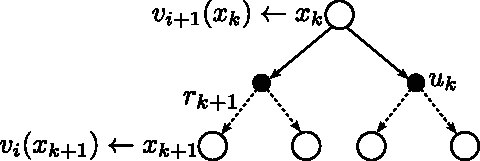
\includegraphics[width=7cm]{fig/lec03/Back_Up_Value_Policy_Evaluation.pdf}
	\caption{Backup diagram for iterative policy evaluation}
	\label{fig:Back_Up_Value_Policy_Evaluation}
\end{figure}
}


%%%%%%%%%%%%%%%%%%%%%%%%%%%%%%%%%%%%%%%%%%%%%%%%%%%%%%%%%%%%%
%% Iterative Policy Evaluation by Richardson Iteration (2)%%
%%%%%%%%%%%%%%%%%%%%%%%%%%%%%%%%%%%%%%%%%%%%%%%%%%%%%%%%%%%%%
\frame{\frametitle{iterative policy evaluation by richardson iteration (2)}
\begin{itemize}
	\item During one Richardson iteration the 'old' value of $x_k$ is replaced with a 'new' value from the 'old' values of the successor state $x_{k+1}$.
	\begin{itemize}
		\item Update $v_{i+1}(x_k)$ from $v_{i}(x_{k+1})$, see \figref{fig:Back_Up_Value_Policy_Evaluation}.
		\item Updating estimates $(v_{i+1})$ on the basis of other estimates $(v_{i})$ is often called \hl{bootstrapping}.
	\end{itemize}\pause
	\item The Richardson iteration can be interpreted as a gradient descent algorithm for solving \eqref{eq:Bellman_matrix_Ab}.\pause
	\item This leads to \hl{synchronous, full backups} of the entire state space $\mathcal{X}$.\pause
	\item Also called \hl{expected update} because it is based on the expectation over all possible next states (utilizing full knowledge).\pause
	\item In subsequent lectures, the expected update will be supplemented by data-driven samples from the environment.
\end{itemize}

}

%%%%%%%%%%%%%%%%%%%%%%%%%%%%%%%%%%%%%%%%%%%%%%%%%%%%%%%%%%%%%
%% Iterative Policy Evaluation Example: Forest Tree MDP%%
%%%%%%%%%%%%%%%%%%%%%%%%%%%%%%%%%%%%%%%%%%%%%%%%%%%%%%%%%%%%%
\frame{\frametitle{iterative policy evaluation example: forest tree mdp}
Let's reuse the forest tree MDP example from \figref{fig:Forest_Markov_Decision_Process_State_Value} with \textit{fifty-fifty policy} and discount factor $\gamma=0.8$
plus disaster probability $\alpha=0.2$:
\begin{equation*}
	\bm{\mathcal{P}}_{xx'}^{\pi} = \begin{bmatrix}0 & \frac{1-\alpha}{2} & 0 & \frac{1+\alpha}{2}  \\ 0 & 0 &\frac{1-\alpha}{2} & \frac{1+\alpha}{2} \\ 0 & 0 &\frac{1-\alpha}{2} & \frac{1+\alpha}{2} \\ 0 & 0 & 0 & 1\end{bmatrix}, \quad\bm{r}_{\mathcal{X}}^{\pi} = \begin{bmatrix}0.5 \\ 1 \\ 2 \\ 0 \end{bmatrix} \, .
\end{equation*}
\pause
\begin{table}
	\centering
		\begin{tabular}{l|l|l|l|l}
			$i$ & $v_i(x=1)$ & $v_i(x=2)$ & $v_i(x=3)$ & $v_i(x=4)$\\
			\hline
			0  & 0 & 0 & 0 & 0\\ \pause
			1  & 0.5 & 1 & 2 &0\\ \pause
			2  & 0.82 & 1.64 & 2.64 & 0\\ \pause
			3  & 1.03 & 1.85 & 2.85 & 0\\ \pause
			\vdots & \vdots & \vdots & \vdots & \vdots \\
			$\infty$ & 1.12 & 1.94 & 2.94 & 0
		\end{tabular}	
	\label{tab:Forest_tree_policy_eval}
	\caption{Policy evaluation by Richardson iteration \eqref{eq:iterative_policy_eval_matrix} for forest tree MDP}
\end{table}
}

%%%%%%%%%%%%%%%%%%%%%%%%%%%%%%%%%%%%%%%%%%%%%%%%%%%%%%%%%%%%%
%% Variant: In-Place Updates %%
%%%%%%%%%%%%%%%%%%%%%%%%%%%%%%%%%%%%%%%%%%%%%%%%%%%%%%%%%%%%%
\frame{\frametitle{variant: in-place updates}
Instead of applying \eqref{eq:iterative_policy_eval_matrix} to the entire vector $\bm{v}_{\mathcal{X},i+1}^{\pi}$ in 'one shot' (synchronous backup), an elementwise \hl{in-place} version of the policy evaluation can be carried out: 
\setlength{\algomargin}{0.5em}
\begin{algorithm}[H]
\SetKwInput{Input}{input} 
\SetKwInput{Output}{output}
\SetKwInput{Init}{init}
\SetKwInput{Param}{parameter}
\Input{full model of the MDP, i.e., $\left\langle\mathcal{X}, \mathcal{U}, \bm{\mathcal{P}}, \mathcal{R}, \gamma \right\rangle$ including policy $\pi$}
\Param{$\delta>0$ as accuracy termination threshold}
\Init{$v_0(x)\, \forall \, x\in\mathcal{X}$ arbitrary except $v_0(x)=0$ if $x$ is terminal}
 \Repeat{$\Delta<\delta$}{
		$\Delta \leftarrow 0 $\;
		\For{$\forall \, x_k\in\mathcal{X}$}{
			$\tilde{v}\leftarrow \hat{v}(x_k)$\;
			$\hat{v}(x_k)\leftarrow  \sum_{u_k\in\mathcal{U}}\pi(u_k|x_k)\left(\mathcal{R}^u_x + \gamma\sum_{x_{k+1}\in\mathcal{X}}p_{xx'}^u \hat{v}(x_{k+1})\right)$\;
			$\Delta \leftarrow \max\left(\Delta, |\tilde{v}-\hat{v}(x_k)|\right)$\;
		}
	}
\caption{
 Iterative policy evaluation using in-place updates (output: estimate of $\bm{v}_{\mathcal{X}}^{\pi}$)}
\label{algo:in_place_policy_update}
\end{algorithm}
}

%%%%%%%%%%%%%%%%%%%%%%%%%%%%%%%%%%%%%%%%%%%%%%%%%%%%%%%%%%%%%
%% In-Place Policy Evaluation Updates for Forest Tree MDP%%
%%%%%%%%%%%%%%%%%%%%%%%%%%%%%%%%%%%%%%%%%%%%%%%%%%%%%%%%%%%%%
\frame{\frametitle{In-place policy evaluation updates for forest tree mdp}
\begin{itemize}
	\item In-place algorithms allow to update states in a beneficial order. \pause
	\item May converge faster than regular Richardson iteration if state update order is chosen wisely (sweep through state space).\pause
	\item For forest tree MDP: reverse order, i.e., start with $x=4$.\pause
	\item As can be seen in \tabref{tab:Forest_tree_policy_eval_in_place} the in-place updates especially converge faster for the 'early states'.
\end{itemize}

\begin{table}
	\centering
		\begin{tabular}{l|l|l|l|l}
			$i$ & $v_i(x=1)$ & $v_i(x=2)$ & $v_i(x=3)$ & $v_i(x=4)$\\
			\hline
			0  & 0 & 0 & 0 & 0\\
			1  & 1.03 & 1.64 & 2 &0\\
			2  & 1.09 & 1.85 & 2.64 & 0\\
			3  & 1.11 & 1.91 & 2.85 & 0\\
			\vdots & \vdots & \vdots & \vdots & \vdots \\
			$\infty$ & 1.12 & 1.94 & 2.94 & 0
		\end{tabular}	
	\caption{In-place updates for forest tree MDP}
	\label{tab:Forest_tree_policy_eval_in_place}
\end{table}
}

%%%%%%%%%%%%%%%%%%%%%%%%%%%%%%%%%%%%%%%%%%%%%%%%%%%%%%%%%%%%%%%%%%
\section{Policy improvement} 
%%%%%%%%%%%%%%%%%%%%%%%%%%%%%%%%%%%%%%%%%%%%%%%%%%%%%%%%%%%%%%%%%%
\begin{frame}
\frametitle{Table of contents}
\tableofcontents[currentsection]
\end{frame}

%%%%%%%%%%%%%%%%%%%%%%%%%%%%%%%%%%%%%%%%%%%%%%%%%%%%%%%%%%%%%
%% General Idea on Policy Improvement%%
%%%%%%%%%%%%%%%%%%%%%%%%%%%%%%%%%%%%%%%%%%%%%%%%%%%%%%%%%%%%%
\frame{\frametitle{General idea on policy improvement}
\vspace{-0.1cm}
\begin{itemize}
	\item If we know $v_{\pi}$ of a given MDP, how to improve the policy?\pause
	\item The simple idea of policy improvement is:
	\begin{itemize}
		\item Consider a new (non-policy conform) action $u\neq{\pi}(x_k)$.
		\item Follow thereafter the current policy $\pi$.
		\item Check the action-value of this 'new move'. If it is better than the 'old' value, take it.
	\end{itemize}
\end{itemize}
	\begin{equation}
	\label{eq:policy_improv_theo01}
			q_\pi(x_k,u_k)	= \E{R_{k+1} + \gamma 	v_{\pi}(X_{k+1})|X_{k}=x_{k},U_{k}=u_{k}}\,.
	\end{equation}\pause\vspace{-0.3cm}
\vspace{-0.1cm}
\begin{theo}{Policy improvement}{Policy_improvement}
If for any deterministic policy pair $\pi$ and $\pi'$
\begin{equation}
\label{eq:policy_improv_theo02}
	q_{\pi}(x,\pi'(x))\geq v_{\pi}(x) \quad \forall x\in\mathcal{X}
\end{equation}
applies, then the policy $\pi'$ must be as good as or better than $\pi$. Hence, it obtains greater or equal expected return
\begin{equation}
\label{eq:policy_improv_theo03}
	v_{\pi'}(x) \geq v_{\pi}(x) \quad \forall x\in\mathcal{X} .
\end{equation}
\end{theo}
}

%%%%%%%%%%%%%%%%%%%%%%%%%%%%%%%%%%%%%%%%%%%%%%%%%%%%%%%%%%%%%
%% Proof of Policy Improvement Theorem %%
%%%%%%%%%%%%%%%%%%%%%%%%%%%%%%%%%%%%%%%%%%%%%%%%%%%%%%%%%%%%%
\frame{\frametitle{Proof of policy improvement theorem}
Start with \eqref{eq:policy_improv_theo02} and recursively reapply \eqref{eq:policy_improv_theo01}:
\begin{equation}
\hspace{-0.35cm}
	\begin{split}
		v_{\pi}(x_k) &\leq q_{\pi}(x_k,\pi'(x_k)),\\
											&= \E{R_{k+1} + \gamma 	v_{\pi}(X_{k+1})|X_{k}=x_{k},U_{k}=\pi'(x_{k})},\\
											&= \El{R_{k+1} + \gamma 	v_{\pi}(X_{k+1})|X_{k}=x_{k}}{\pi'},\\
											&\leq \El{R_{k+1} + \gamma 	q_{\pi}(x_{k+1},\pi'(x_{k+1}))|X_{k}=x_{k}}{\pi'},\\
											&= \El{R_{k+1} + \gamma 	\El{R_{k+2} + \gamma 	v_{\pi}(X_{k+2})|X_{k+1},\pi'(x_{k+1})}{\pi'}|X_{k}=x_{k}}{\pi'},\\
											&= \El{R_{k+1} + \gamma 	R_{k+2} + \gamma^2 v_{\pi}(X_{k+2})|X_{k}=x_{k}}{\pi'},\\
											&\leq \El{R_{k+1} + \gamma 	R_{k+2} + \gamma^2 R_{k+3}+ \gamma^3 v_{\pi}(X_{k+3})|X_{k}=x_{k}}{\pi'},\\
											&\hspace{0.2cm}\vdots\\
											&\leq \El{R_{k+1} + \gamma 	R_{k+2} + \gamma^2 R_{k+3}+ \gamma^3 R_{k+4}+\cdots|X_{k}=x_{k}}{\pi'},\\
											&=v_{\pi'}(x_k).
	\end{split}
\end{equation}
}

%%%%%%%%%%%%%%%%%%%%%%%%%%%%%%%%%%%%%%%%%%%%%%%%%%%%%%%%%%%%%
%% Greedy Policy Improvement (1) %%
%%%%%%%%%%%%%%%%%%%%%%%%%%%%%%%%%%%%%%%%%%%%%%%%%%%%%%%%%%%%%
\frame{\frametitle{greedy policy improvement (1)}
\begin{itemize}
	\item So far, policy improvement addressed only changing the policy at a single state.\pause
	\item Now, extend this scheme to all states by selecting the best action according to $q_\pi(x_{k}, u_{k})$ in every state (\hl{greedy policy improvement}):\pause
\end{itemize}
\vspace{0.25cm}
\begin{equation}
	\begin{split}
		\pi'(x_{k})&	=\argmax_{u_k\in\mathcal{U}} q_\pi(x_{k}, u_{k}),\\
										& = \argmax_{u_k\in\mathcal{U}} \E{R_{k+1} + \gamma 	v_{\pi}(X_{k+1})|X_{k}=x_{k},U_{k}=u_{k}},\\
										& = \argmax_{u_k\in\mathcal{U}} \mathcal{R}^u_x + \gamma \sum_{x_{k+1}\in\mathcal{X}}p_{xx'}^u v_\pi(x_{k+1}) \, .
	\end{split}
\end{equation}
\begin{itemize}
	\item Again, consider that $\mathcal{R}^u_x$ could be of deterministic or stochastic nature.
\end{itemize}
}

%%%%%%%%%%%%%%%%%%%%%%%%%%%%%%%%%%%%%%%%%%%%%%%%%%%%%%%%%%%%%
%% Greedy Policy Improvement (2) %%
%%%%%%%%%%%%%%%%%%%%%%%%%%%%%%%%%%%%%%%%%%%%%%%%%%%%%%%%%%%%%
\frame{\frametitle{greedy policy improvement (2)}
\begin{itemize}
	\item Each greedy policy improvement takes the best action in a one-step look-ahead search and, therefore, satisfies \theoref{theo:Policy_improvement}.\pause
	\item If after a policy improvement step $v_{\pi}(x_k) = v_{\pi'}(x_k)$ applies, it follows:
\end{itemize}
\vspace{0.25cm}
\begin{equation}
	\begin{split}
		v_{\pi'}(x_k) &=	\max_{u_k\in\mathcal{U}} \E{R_{k+1} + \gamma 	v_{\pi'}(X_{k+1})|X_{k}=x_{k},U_{k}=u_{k}},\\
										& = \max_{u_k\in\mathcal{U}} \mathcal{R}^u_x + \gamma \sum_{x_{k+1}\in\mathcal{X}}p_{xx'}^u v_{\pi'}(x_{k+1}) \, .
	\end{split}
\end{equation}\pause
\begin{itemize}
	\item This is the Bellman optimality equation, which guarantees that $\pi'=\pi$ must be optimal policies.\pause
	\item Although proof for policy improvement theorem was presented for deterministic policies, transfer to stochastic policies $\pi(u_k|x_k)$ is possible.\pause
	\item Takeaway message: \hl{policy improvement theorem guarantees finding optimal policies in finite MDPs} (e.g., by DP).
\end{itemize}	
}

%%%%%%%%%%%%%%%%%%%%%%%%%%%%%%%%%%%%%%%%%%%%%%%%%%%%%%%%%%%%%%%%%%
\section{Policy and value iteration} 
%%%%%%%%%%%%%%%%%%%%%%%%%%%%%%%%%%%%%%%%%%%%%%%%%%%%%%%%%%%%%%%%%%
\begin{frame}
\frametitle{Table of contents}
\tableofcontents[currentsection]
\end{frame}

%%%%%%%%%%%%%%%%%%%%%%%%%%%%%%%%%%%%%%%%%%%%%%%%%%%%%%%%%%%%%
%% Concept of Policy Iteration %%
%%%%%%%%%%%%%%%%%%%%%%%%%%%%%%%%%%%%%%%%%%%%%%%%%%%%%%%%%%%%%
\frame{\frametitle{Concept of policy iteration}
\begin{itemize}
	\item Policy iteration \hl{combines the previous policy evaluation and policy improvement} in an iterative sequence: 
\end{itemize}
\vspace{0.25cm}
\begin{equation}
\label{eq:policy_iter}
	\pi_0 \rightarrow v_{\pi_0} \rightarrow \pi_1 \rightarrow v_{\pi_1} \rightarrow \cdots \pi^* \rightarrow v_{\pi^*}
\end{equation}
\begin{itemize}
	\item Evaluate $\rightarrow$ improve $\rightarrow$ evaluate $\rightarrow$ improve ...\pause
	\item In the 'classic' policy iteration, each policy evaluation step in \eqref{eq:policy_iter} is fully executed, i.e., for each policy $\pi_i$ an exact estimate of $v_{\pi_i}$ is provided either by iterative policy evaluation with a sufficiently high number of steps or by any other method that fully solves \eqref{eq:Bellman_matrix_Ab}.
\end{itemize}
}

%%%%%%%%%%%%%%%%%%%%%%%%%%%%%%%%%%%%%%%%%%%%%%%%%%%%%%%%%%%%%
%% Policy Iteration Example: Forest Tree MDP (1) %%
%%%%%%%%%%%%%%%%%%%%%%%%%%%%%%%%%%%%%%%%%%%%%%%%%%%%%%%%%%%%%
\frame{\frametitle{policy iteration example: forest tree mdp (1)}
\begin{figure}		
	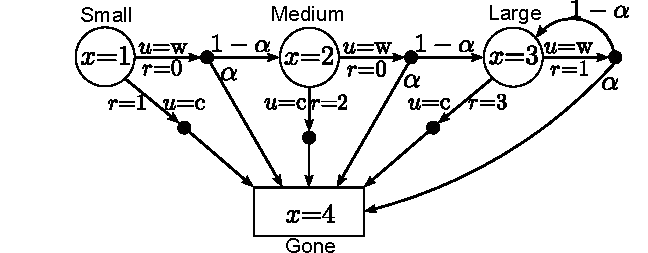
\includegraphics[width=11cm]{fig/lec03/Forest_Markov_Decision_Process.pdf}
\end{figure}
\begin{itemize}
	\item Two actions possible in each state:
	\begin{itemize}
		\item Wait $u=w$: let the tree grow.
		\item Cut $u=c$: gather the wood.
	\end{itemize}
\end{itemize}
}

%%%%%%%%%%%%%%%%%%%%%%%%%%%%%%%%%%%%%%%%%%%%%%%%%%%%%%%%%%%%%
%% Policy Iteration Example: Forest Tree MDP (2) %%
%%%%%%%%%%%%%%%%%%%%%%%%%%%%%%%%%%%%%%%%%%%%%%%%%%%%%%%%%%%%%
\frame{\frametitle{policy iteration example: forest tree mdp (2)}
Assume $\alpha=0.2$ and $\gamma=0.8$ and start with \hl{'tree hater' initial policy}:\pause
\begin{enumerate}
	\item $\pi_0=\pi(u_k =\mbox{c}|x_k) \quad \,\forall x_k\in\mathcal{X}$.\pause
	\item Policy evaluation: $v_\mathcal{X}^{\pi_0}=\begin{bmatrix}1 & 2 & 3 & 0\end{bmatrix}^T$\pause
	\item Greedy policy improvement: 
	\begin{equation*}
	\begin{split}
		\pi_1(x_{k})& = \argmax_{u_k\in\mathcal{U}} \E{R_{k+1} + \gamma 	v_{\pi_0}(X_{k+1})|X_{k}=x_{k},U_{k}=u_{k}},\\
										& = \left\{\pi(u_k =\mbox{w}|x_k=1), \pi(u_k =\mbox{c}|x_k=2), \pi(u_k =\mbox{c}|x_k=3)\right\}
	\end{split}
\end{equation*}\pause
\item Policy evaluation: $v_\mathcal{X}^{\pi_1}=\begin{bmatrix}1.28 & 2 & 3 & 0\end{bmatrix}^T$\pause
\item Greedy policy improvement: 
	\begin{equation*}
	\begin{split}
		\pi_2(x_{k})& = \argmax_{u_k\in\mathcal{U}} \E{R_{k+1} + \gamma 	v_{\pi_1}(X_{k+1})|X_{k}=x_{k},U_{k}=u_{k}},\\
										& = \left\{\pi(u_k =\mbox{w}|x_k=1), \pi(u_k =\mbox{c}|x_k=2), \pi(u_k =\mbox{c}|x_k=3)\right\},\\
										& = \pi_1(x_{k})\\
										& = \pi^*
	\end{split}
\end{equation*}
\end{enumerate}
}

%%%%%%%%%%%%%%%%%%%%%%%%%%%%%%%%%%%%%%%%%%%%%%%%%%%%%%%%%%%%%
%% Policy Iteration Example: Forest Tree MDP (3) %%
%%%%%%%%%%%%%%%%%%%%%%%%%%%%%%%%%%%%%%%%%%%%%%%%%%%%%%%%%%%%%
\frame{\frametitle{policy iteration example: forest tree mdp (3)}
Assume $\alpha=0.2$ and $\gamma=0.8$ and start with \hl{'tree lover' initial policy}:\pause
\begin{enumerate}
	\item $\pi_0=\pi(u_k =\mbox{w}|x_k) \quad \,\forall x_k\in\mathcal{X}$.\pause
	\item Policy evaluation: $v_\mathcal{X}^{\pi_0}=\begin{bmatrix}1.14 & 1.78 & 2.78 & 0\end{bmatrix}^T$\pause
	\item Greedy policy improvement: 
	\begin{equation*}
	\begin{split}
		\pi_1(x_{k})& = \argmax_{u_k\in\mathcal{U}} \E{R_{k+1} + \gamma 	v_{\pi_0}(X_{k+1})|X_{k}=x_{k},U_{k}=u_{k}},\\
										& = \left\{\pi(u_k =\mbox{w}|x_k=1), \pi(u_k =\mbox{c}|x_k=2), \pi(u_k =\mbox{c}|x_k=3)\right\}
	\end{split}
\end{equation*}\pause
\item Policy evaluation: $v_\mathcal{X}^{\pi_1}=\begin{bmatrix}1.28 & 2 & 3 & 0\end{bmatrix}^T$\pause
\item Greedy policy improvement: 
	\begin{equation*}
	\begin{split}
		\pi_2(x_{k})& = \argmax_{u_k\in\mathcal{U}} \E{R_{k+1} + \gamma 	v_{\pi_1}(X_{k+1})|X_{k}=x_{k},U_{k}=u_{k}},\\
										& = \left\{\pi(u_k =\mbox{w}|x_k=1), \pi(u_k =\mbox{c}|x_k=2), \pi(u_k =\mbox{c}|x_k=3)\right\},\\
										& = \pi_1(x_{k})\\
										& = \pi^*
	\end{split}
\end{equation*}
\end{enumerate}
}

%%%%%%%%%%%%%%%%%%%%%%%%%%%%%%%%%%%%%%%%%%%%%%%%%%%%%%%%%%%%%
%% Policy Iteration Example: Jack's Car Rental (1) %%
%%%%%%%%%%%%%%%%%%%%%%%%%%%%%%%%%%%%%%%%%%%%%%%%%%%%%%%%%%%%%
\frame{\frametitle{policy iteration example: jack's car rental (1)}
\begin{figure}		
	\includegraphics[width=2cm]{fig/lec03/car_rental.pdf}
\end{figure}
\begin{itemize}
	\item States: Two rental locations, maximum of 20 cars each\pause
	\item Actions: Move up to 5 cars between locations overnight\pause
	\item Reward: 
	\begin{itemize}
		\item  +10 \$ for each car rented (if available at location)
		\item -2 \$ for each overnight car transfer
		\item Discount: $\gamma=0.9$
	\end{itemize}\pause 
	\item Dynamics: Cars returned and requested randomly following Poisson distribution
	\begin{itemize}
		\item $P_\lambda(n)=\frac{\lambda^n}{n!}e^{-\lambda}$
		\item $P_\lambda(n)=$ probability of observing $n$ events with mean event rate $\lambda$
		\item 1st location: $\lambda_{\mbox{req.}}=3$, $\lambda_{\mbox{ret.}}=3$
		\item 2nd location: $\lambda_{\mbox{req.}}=4$, $\lambda_{\mbox{ret.}}=2$
	\end{itemize}
\end{itemize}
}

%%%%%%%%%%%%%%%%%%%%%%%%%%%%%%%%%%%%%%%%%%%%%%%%%%%%%%%%%%%%%
%% Policy Iteration Example: Jack's Car Rental (2) %%
%%%%%%%%%%%%%%%%%%%%%%%%%%%%%%%%%%%%%%%%%%%%%%%%%%%%%%%%%%%%%
\frame{\frametitle{policy iteration example: jack's car rental (2)}
\begin{figure}
		\includegraphics[width=9cm]{fig/lec03/Jack_Car_Rental.pdf}
		\caption{Sequence of policies found by policy iteration including optimal state value after termination (source: R. Sutton and G. Barto, Reinforcement learning: an introduction, 2018, \href{https://creativecommons.org/licenses/by-nc-nd/2.0/}{CC BY-NC-ND 2.0})}
		\label{fig:Jack_Car_Rental}
	\end{figure}
}

%%%%%%%%%%%%%%%%%%%%%%%%%%%%%%%%%%%%%%%%%%%%%%%%%%%%%%%%%%%%%
%% Value Iteration (1) %%
%%%%%%%%%%%%%%%%%%%%%%%%%%%%%%%%%%%%%%%%%%%%%%%%%%%%%%%%%%%%%
\frame{\frametitle{value iteration (1)}
\begin{itemize}
	\item Policy iteration involves full policy evaluation steps between policy improvements.
	\item In large state-space MDPs the full policy evaluation may be numerically very costly.\pause
	\item Using a limited number of iterative policy evaluations steps and then apply policy improvement may speed up the entire DP process.\pause
	\item \hl{Value iteration}: One step iterative policy evaluation followed by policy improvement.\pause
	\item Allows simple update rule which \hl{combines policy improvement with truncated policy evaluation}:
	\begin{equation}
	\begin{split}
		v_{i+1}(x_k) &=	\max_{u_k\in\mathcal{U}} \E{R_{k+1} + \gamma 	v_{i}(X_{k+1})|X_{k}=x_{k},U_{k}=u_{k}},\\
										&= \max_{u_k\in\mathcal{U}} \mathcal{R}^u_x + \gamma \sum_{x_{k+1}\in\mathcal{X}}p_{xx'}^u v_{i}(x_{k+1}) \, .
	\end{split}
\end{equation}
\end{itemize}
}

%%%%%%%%%%%%%%%%%%%%%%%%%%%%%%%%%%%%%%%%%%%%%%%%%%%%%%%%%%%%%
%% Value Iteration (2) %%
%%%%%%%%%%%%%%%%%%%%%%%%%%%%%%%%%%%%%%%%%%%%%%%%%%%%%%%%%%%%%
\frame{\frametitle{value iteration (2)}
\setlength{\algomargin}{0.5em}
\begin{algorithm}[H]
\SetKwInput{Input}{input} 
\SetKwInput{Output}{output}
\SetKwInput{Init}{init}
\SetKwInput{Param}{parameter}
\Input{full model of the MDP, i.e., $\left\langle\mathcal{X}, \mathcal{U}, \bm{\mathcal{P}}, \mathcal{R}, \gamma \right\rangle$}
\Param{$\delta>0$ as accuracy termination threshold}
\Init{$v_0(x)\, \forall \, x\in\mathcal{X}$ arbitrary except $v_0(x)=0$ if $x$ is terminal}
 \Repeat{$\Delta<\delta$}{
		$\Delta \leftarrow 0 $\;
		\For{$\forall \, x_k\in\mathcal{X}$}{
			$\tilde{v}\leftarrow \hat{v}(x_k)$\;
			$\hat{v}(x_k)\leftarrow  \max_{u_k\in\mathcal{U}}\left(\mathcal{R}^u_x + \gamma\sum_{x_{k+1}\in\mathcal{X}}p_{xx'}^u \hat{v}(x_{k+1})\right)$\;
			$\Delta \leftarrow \max\left(\Delta, |\tilde{v}-\hat{v}(x_k)|\right)$\;
		}
	}
\Output{Deterministic policy $\pi\approx\pi^*$, such that}
	$\pi(x_k)\leftarrow  \argmax_{u_k\in\mathcal{U}}\left(\mathcal{R}^u_x + \gamma\sum_{x_{k+1}\in\mathcal{X}}p_{xx'}^u \hat{v}(x_{k+1})\right)$\;
\caption{Value iteration (note: compared to policy iteration, value iteration doesn't require an initial policy but only a state-value guess)}
\end{algorithm}
}

%%%%%%%%%%%%%%%%%%%%%%%%%%%%%%%%%%%%%%%%%%%%%%%%%%%%%%%%%%%%%
%% Value Iteration for Forest Tree MDP %%
%%%%%%%%%%%%%%%%%%%%%%%%%%%%%%%%%%%%%%%%%%%%%%%%%%%%%%%%%%%%%
\frame{\frametitle{Value iteration for forest tree mdp}
\begin{figure}		
	\includegraphics[width=6cm]{fig/lec03/Forest_Markov_Decision_Process.pdf}
\end{figure}
\begin{itemize}
	\item Assume again $\alpha=0.2$ and $\gamma=0.8$.\pause
	\item Similar to in-place update policy evaluation, reverse order and start value iteration with $x=4$.\pause
	\item As shown in \tabref{tab:Forest_tree_value_iteration} value iteration converges in one step (for the given problem) to the optimal state-value. 
\end{itemize}
\begin{table}
	\centering
		\begin{tabular}{l|l|l|l|l}
			$i$ & $v_i(x=1)$ & $v_i(x=2)$ & $v_i(x=3)$ & $v_i(x=4)$\\
			\hline
			0  & 0 & 0 & 0 & 0\\
			1  & 1.28 & 2 & 3 &0\\
			*  & 1.28 & 2 & 3 &0
		\end{tabular}	
	\caption{Value iteration for forest tree MDP}
	\label{tab:Forest_tree_value_iteration}
\end{table}
}


%%%%%%%%%%%%%%%%%%%%%%%%%%%%%%%%%%%%%%%%%%%%%%%%%%%%%%%%%%%%%%%%%%
\section{Further aspects} 
%%%%%%%%%%%%%%%%%%%%%%%%%%%%%%%%%%%%%%%%%%%%%%%%%%%%%%%%%%%%%%%%%%
\begin{frame}
\frametitle{Table of contents}
\tableofcontents[currentsection]
\end{frame}

%%%%%%%%%%%%%%%%%%%%%%%%%%%%%%%%%%%%%%%%%%%%%%%%%%%%%%%%%%%%%
%% Summarizing DP Algorithms %%
%%%%%%%%%%%%%%%%%%%%%%%%%%%%%%%%%%%%%%%%%%%%%%%%%%%%%%%%%%%%%
\frame{\frametitle{Summarizing dp algorithms}
\begin{itemize}
	\item All DP algorithms are based on the state-value $v(x)$.
	\begin{itemize}
		\item Complexity is $\mathcal{O}(m\cdot n^2)$ for $m$ actions and $n$ states.
		\item Evaluate all $n^2$ state transitions while considering up to $m$ actions per state.
	\end{itemize}\pause
	\item Could be also applied to action-values $q(x,u)$.
	\begin{itemize}
		\item Complexity is inferior with $\mathcal{O}(m^2\cdot n^2)$.
		\item There are up to $m^2$ action-values which require $n^2$ state transition evaluations each.
	\end{itemize}
\end{itemize}
\pause
\begin{table}
	\centering
		\begin{tabular}{|M{1.65cm}||M{4.75cm}|M{4cm}|}
			\hline
			Problem & Relevant Equations & Algorithm\\
			\hline\hline
			prediction & Bellman expectation eq. &  policy evaluation\\
			\hline
			control & Bellman expectation eq. \& greedy policy improvement & policy iteration\\
			\hline
			control & Bellman optimality eq. & value iteration\\
			\hline
		\end{tabular}	
		\caption{Short overview addressing the treated DP algorithms}
		\label{tab:DP_syn_algos}
\end{table}
}

%%%%%%%%%%%%%%%%%%%%%%%%%%%%%%%%%%%%%%%%%%%%%%%%%%%%%%%%%%%%%
%%Asynchronous DP%%
%%%%%%%%%%%%%%%%%%%%%%%%%%%%%%%%%%%%%%%%%%%%%%%%%%%%%%%%%%%%%
\frame{\frametitle{Asynchronous dp}
\begin{itemize}
	\item DP algorithms considered so far used \hl{synchronous backups}:
	\begin{itemize}
		\item In one iteration the entire state space is updated.
		\item May be computational expensive for large MDPs.
		\item Some state-values or policy parts may converge faster than other but are updated as often as slowly converging states.
	\end{itemize}
	\vspace{0.5cm}\pause
	\item In contrast, \hl{asynchronous backups} update states individually in an (arbitrary) order:
	\begin{itemize}
		\item Choose smart order to achieve faster overall convergence rate.
		\item Some states may be updated more frequently than others.\pause
		\item Overall algorithms converges if all states are still visited to some extent (\hl{important requirement to ensure convergence}).\pause
		\item Simple example: in-place policy evaluation where only a subset of all states are updated each iterations (cf. \algoref{algo:in_place_policy_update}).
	\end{itemize}
\end{itemize}
}

%%%%%%%%%%%%%%%%%%%%%%%%%%%%%%%%%%%%%%%%%%%%%%%%%%%%%%%%%%%%%
%% Asynchronous DP: Prioritized Sweeping %%
%%%%%%%%%%%%%%%%%%%%%%%%%%%%%%%%%%%%%%%%%%%%%%%%%%%%%%%%%%%%%
\frame{\frametitle{asynchronous dp: prioritized sweeping}
\begin{itemize}
	\item Use magnitude of \hl{Bellman error} as an indicator which state should be updated next:
	\begin{equation}
		\argmax_{x_k\in\mathcal{X}}\left|\max_{u_k\in\mathcal{U}} \left(\mathcal{R}^u_x + \gamma \sum_{x_{k+1}\in\mathcal{X}}p_{xx'}^u v_{i}(x_{k+1})\right) - v_i(x_k)\right|\, .
	\end{equation}\pause
	\item Update the state with the largest Bellman error first. 
	\item Build up a priority queue of most relevant states by refreshing the Bellman error after each state update.
\end{itemize}
}

%%%%%%%%%%%%%%%%%%%%%%%%%%%%%%%%%%%%%%%%%%%%%%%%%%%%%%%%%%%%%
%% Asynchronous DP: Real-Time Updates %%
%%%%%%%%%%%%%%%%%%%%%%%%%%%%%%%%%%%%%%%%%%%%%%%%%%%%%%%%%%%%%
\frame{\frametitle{asynchronous dp: real-time updates}
\begin{itemize}
	\item Update those states which are frequently visited by the agent.
	\item Utilizes agent's experience to guide the asynchronous DP updates.
	\item After each time step $\left\langle x_k, u_k, r_{k+1}\right\rangle$ update $x_k$:
	\begin{equation}
		v_i(x_k) \leftarrow \max_{u_k\in\mathcal{U}} \left(\mathcal{R}^u_{x} + \gamma \sum_{x_{k+1}\in\mathcal{X}}p_{xx'}^u v_{i}(x_{k+1})\right).
	\end{equation}
\end{itemize}
\begin{figure}
		\includegraphics[width=5.5cm]{fig/lec03/RTDP.pdf}
		\caption{Real-time DP updates focus on reachable states (source: R. Sutton and G. Barto, Reinforcement learning: an introduction, 2018, \href{https://creativecommons.org/licenses/by-nc-nd/2.0/}{CC BY-NC-ND 2.0})}
		\label{fig:RTDP}
\end{figure}
}

%%%%%%%%%%%%%%%%%%%%%%%%%%%%%%%%%%%%%%%%%%%%%%%%%%%%%%%%%%%%%
%% Generalized Policy Iteration %%
%%%%%%%%%%%%%%%%%%%%%%%%%%%%%%%%%%%%%%%%%%%%%%%%%%%%%%%%%%%%%
\frame{\frametitle{generalized policy iteration (gpi)}
\begin{itemize}
	\item Almost all RL methods are well-described as GPI.
	\item \hl{Push-pull}: Improving the policy will deteriorate value estimation.  
	\item Well balanced \hl{trade-off between evaluating and improving} is required.
\end{itemize}
\begin{figure}
	\subfloat{
		\includegraphics[height=4cm]{fig/lec03/GPI_01.pdf}
	}
	\hspace{1cm}
	\subfloat{
		\includegraphics[height=4cm]{fig/lec03/GPI_02.pdf}
	}
\caption{Interpreting generalized policy iteration to switch back and forth between (arbitrary) evaluations and improvement steps (source: R. Sutton and G. Barto, Reinforcement learning: an introduction, 2018, \href{https://creativecommons.org/licenses/by-nc-nd/2.0/}{CC BY-NC-ND 2.0})}
\end{figure}
}

%%%%%%%%%%%%%%%%%%%%%%%%%%%%%%%%%%%%%%%%%%%%%%%%%%%%%%%%%%%%%
%% Curse of Dimensionality %%
%%%%%%%%%%%%%%%%%%%%%%%%%%%%%%%%%%%%%%%%%%%%%%%%%%%%%%%%%%%%%
\frame{\frametitle{Curse of dimensionality}
\begin{itemize}
	\item DP is much more efficient than an exhaustive search over all $n$ states and $m$ actions in finite MDPs in order to find an optimal policy.
	\begin{itemize}
		\item Exhaustive search for deterministic policies: $m^n$ evaluations.
		\item DP results in polynomial complexity regarding $m$ and $n$. 
	\end{itemize}
	\pause
	\item Nevertheless, DP uses full-width backups:
	\begin{itemize}
		\item For each state update, every successor state and action is considered.
		\item While utilizing full knowledge of the MDP structure.
	\end{itemize}
	\pause
	\item Hence, DP is can be effective up to medium-sized MDPs (i.e., million states)\pause
	\item For large problems DP suffers from the \hl{curse of dimensionality}:
	\begin{itemize}
		\item Number of finite states $n$ grows exponentially with the number of state variables.
		\item Also: if continuous variables need quantization typically a large number of states results. 
		\item Single state update may become computational infeasible. 
	\end{itemize}
\end{itemize}
}

%%%%%%%%%%%%%%%%%%%%%%%%%%%%%%%%%%%%%%%%%%%%%%%%%%%%%%%%%%%%%
%% Summary %%
%%%%%%%%%%%%%%%%%%%%%%%%%%%%%%%%%%%%%%%%%%%%%%%%%%%%%%%%%%%%%
\begin{frame}
\frametitle{summary: what you've learned today}
\begin{itemize}
	\item DP is applicable for prediction and control problems in MDPs.\pause
	\item But requires always full knowledge about the environment (i.e., it is a model-based solution also called planning).\pause
	\item DP is more efficient than exhaustive search.\pause
	\item But suffers from the curse of dimensionality for large MDPs.\pause
	\item (Iterative) policy evaluations and (greedy) improvements solve MDPs.\pause
	\item Both steps can be combined via value iteration.\pause
	\item This idea of (generalized) policy iteration is a basic scheme of RL.\pause
	\item Implementing DP algorithms comes with many degrees of freedom.
	\item For example how to order the state updates (asyn. vs. sync.).
\end{itemize}
\end{frame}

\part{Lecture 04: Monte Carlo Methods}
\title[RL Lecture 04]{Lecture 04: Monte Carlo Methods}  
\date{}  
\frame{\titlepage} 
\frame{\frametitle{Table of Contents}\tableofcontents} 

%%%%%%%%%%%%%%%%%%%%%%%%%%%%%%%%%%%%%%%%%%%%%%%%%%%%%%%%%%%%%%%%%%
\section{General Idea and Differences to Dynamic Programming} 
%%%%%%%%%%%%%%%%%%%%%%%%%%%%%%%%%%%%%%%%%%%%%%%%%%%%%%%%%%%%%%%%%%

%%%%%%%%%%%%%%%%%%%%%%%%%%%%%%%%%%%%%%%%%%%%%%%%%%%%%%%%%%%%%
%% Monte Carlo Methods vs. Dynamic Programming %%
%%%%%%%%%%%%%%%%%%%%%%%%%%%%%%%%%%%%%%%%%%%%%%%%%%%%%%%%%%%%%
\frame{\frametitle{Monte Carlo Methods vs. Dynamic Programming}
Dynamic Programming:
\begin{itemize}
	\item \hl{Model-based} prediction and control 
	\item Planning inside \hl{known MDPs}
\end{itemize}
\vspace{1cm}
\pause
Monte Carlo methods:
\begin{itemize}
	\item \hl{Model-free} prediction and control
	\item Estimating value functions and optimize policies in \hl{unknown MDPs}
	\item But: still assuming finite MDP problems (or problems close to that)
	\item In general: broad class of computational algorithms relying on \hl{repeated random sampling} to obtain numerical results
\end{itemize}
}

%%%%%%%%%%%%%%%%%%%%%%%%%%%%%%%%%%%%%%%%%%%%%%%%%%%%%%%%%%%%%
%% General Monte Carlo Methods' Characteristics %%
%%%%%%%%%%%%%%%%%%%%%%%%%%%%%%%%%%%%%%%%%%%%%%%%%%%%%%%%%%%%%
\frame{\frametitle{General Monte Carlo (MC) Methods' Characteristics}
\begin{itemize}
	\onslide<1->\item \hl{Learning  from experience}, i.e., sequences of samples $\left\langle x_k, u_k, r_{k+1}\right\rangle$
	\onslide<2->\item Main concept: Estimation by \hl{averaging sample returns}
	\onslide<3->\item To guarantee well-defined returns: \hl{limited to episodic tasks}
	\onslide<4->\item Consequence: Estimation and policy updates only possible in an episode-by-episode way compared to step-by-step (online)
\end{itemize}
\onslide<1->\begin{figure}
\includegraphics[width=8cm]{fig/lec04/Monte_Carlo_City.jpg}
\caption{Monte Carlo port \\(source: \href{https://www.flickr.com/photos/flynn_nrg/40890124713/}{www.flickr.com}, by \href{https://www.flickr.com/photos/flynn_nrg/}{Miguel Mendez} \href{https://creativecommons.org/licenses/by/2.0/}{CC BY 2.0})}
\label{fig:MMonte_Carlo_City}
\end{figure}
}

%%%%%%%%%%%%%%%%%%%%%%%%%%%%%%%%%%%%%%%%%%%%%%%%%%%%%%%%%%%%%%%%%%
\section{Basic Monte Carlo Prediction} 
%%%%%%%%%%%%%%%%%%%%%%%%%%%%%%%%%%%%%%%%%%%%%%%%%%%%%%%%%%%%%%%%%%
\begin{frame}
\frametitle{Table of Contents}
\tableofcontents[currentsection]
\end{frame}

%%%%%%%%%%%%%%%%%%%%%%%%%%%%%%%%%%%%%%%%%%%%%%%%%%%%%%%%%%%%%
%% Task Description and Basic Solution %%
%%%%%%%%%%%%%%%%%%%%%%%%%%%%%%%%%%%%%%%%%%%%%%%%%%%%%%%%%%%%%
\frame{\frametitle{Task Description and Basic Solution}
\begin{block}{MC prediction problem statement}
\begin{itemize}
	\item Estimate state value $v_{\pi}(x)$ for a given policy $\pi$.
	\item Available are samples $\left\langle x_{k,j}, u_{k,j}, r_{k+1,j}\right\rangle$ for episodes  $j=1,\ldots,J$.
\end{itemize}
\end{block}
\pause
\vspace{0.25cm}
MC solution approach:
\begin{itemize}
	\item Average returns after visiting state $x_k$ over episodes $j=1,\ldots$
	\begin{equation}
		v_{\pi}(x_k) \approx \hat{v}_{\pi}(x_k)=\frac{1}{J}\sum_{j=1}^J g_{k,j}=\frac{1}{J}\sum_{j=1}^J\sum_{i=0}^{T_j} \gamma^i r_{k+i+1,j}\, .
		\label{eq:MC_average_v_basic}
	\end{equation}
	\item Above, $T_j$ denotes the \hl{terminating time step} of each episode $j$.\pause
	\item \hl{First-visit MC}: Apply \eqref{eq:MC_average_v_basic} only to the first state visit per episode.\pause
	\item \hl{Every-visit MC}: Apply \eqref{eq:MC_average_v_basic} each time visiting a certain state per episode (if a state is visited more than one time per episode).
\end{itemize}
}

%%%%%%%%%%%%%%%%%%%%%%%%%%%%%%%%%%%%%%%%%%%%%%%%%%%%%%%%%%%%%
%% Algorithmic Implementation:MC-Based Prediction %%
%%%%%%%%%%%%%%%%%%%%%%%%%%%%%%%%%%%%%%%%%%%%%%%%%%%%%%%%%%%%%
\frame{\frametitle{Algorithmic Implementation: MC-Based Prediction}
\setlength{\algomargin}{0.5em}
\begin{algorithm}[H]
\SetKwInput{Input}{input} 
\SetKwInput{Output}{output}
\SetKwInput{Init}{init}
\SetKwInput{Param}{parameter}
\Input{a policy $\pi$ to be evaluated}
\Output{estimate of $\bm{v}_{\mathcal{X}}^{\pi}$ (i.e., value estimate for all states				 $x\in\mathcal{X}$)}
\Init{$\hat{v}(x)\, \forall \, x\in\mathcal{X}$ arbitrary except $v_0(x)=0$ if $x$ is terminal\newline 
$l(x)\leftarrow$ an empty list for every $x\in\mathcal{X}$}
 \For{$j=1,\ldots,J$ episodes}{
		Generate an episode following $\pi$: $x_{0}, u_{0}, r_{1},\ldots,x_{T_j}, u_{T_j}, r_{T_{j}+1}$ \;
		Set $g \leftarrow 0$\;
		\For{$k=T_j-1, T_j-2, T_j-3,\ldots, 0$ time steps}{
			$g \leftarrow \gamma g + r_{k+1}$\;
			\If{$x_{k}\notin \left\langle x_{0}, x_{1}, \ldots, x_{k-1}\right\rangle$}{
					Append $g$ to list $l(x_k)$\;
					$\hat{v}(x_k)\leftarrow \mbox{average}(\,l(x_k)\,)$\;}
		}
	}
\caption{First-visit MC state-value prediction}
\label{algo:MC_state_prediction_first_visit}
\end{algorithm}
}

%%%%%%%%%%%%%%%%%%%%%%%%%%%%%%%%%%%%%%%%%%%%%%%%%%%%%%%%%%%%%
%% Incremental Implementation%%
%%%%%%%%%%%%%%%%%%%%%%%%%%%%%%%%%%%%%%%%%%%%%%%%%%%%%%%%%%%%%
\frame{\frametitle{Incremental Implementation}
\begin{itemize}
	\item \algoref{algo:MC_state_prediction_first_visit} is inefficient due to large memory demand.
	\item Better: use \hl{incremental / recursive implementation}.\pause
	\item The sample mean $\mu_1,\mu_2,\ldots$ of an arbitrary sequence $g_1, g_2, \ldots$ is:
\end{itemize}
\begin{equation}
	\begin{split}
		\mu_j &= \frac{1}{j}\sum_{i=1}^j g_i,\\
					&= \frac{1}{j}\left[g_j + \sum_{i=1}^{j-1} g_i\right],\\
					&= \frac{1}{j}\left[g_j + (j-1) \mu_{j-1}\right],\\
					&=\mu_{j-1} + \frac{1}{j}\left[g_j-\mu_{j-1}\right].
	\end{split}
	\label{eq:inc_impl_MC_pred}
\end{equation} \pause
\begin{itemize}
	\item \hl{If a given decision problem is non-stationary}, using a forgetting factor $\alpha\in\left\{\mathbb{R}|0<\alpha<1\right\}$ allows for dynamic adaption: 
\end{itemize}
\begin{equation}
	\mu_j = \mu_{j-1} + \alpha\left[g_j-\mu_{j-1}\right] .
	\label{eq:inc_impl_MC_pred_non_stat}
\end{equation}
}

%%%%%%%%%%%%%%%%%%%%%%%%%%%%%%%%%%%%%%%%%%%%%%%%%%%%%%%%%%%%%
%% Statistical Properties of MC-Based Prediction (1)%%
%%%%%%%%%%%%%%%%%%%%%%%%%%%%%%%%%%%%%%%%%%%%%%%%%%%%%%%%%%%%%
\frame{\frametitle{Statistical Properties of MC-Based Prediction (1)}
\onslide<1->{First-time visit MC:
\begin{itemize}
	\item Each return sample $g_j$ is independent from the others since they were drawn from separate episodes.   
	\item One receives \hl{i.i.d. data} to estimate $\E{\hat{v}_{\pi}}$ and consequently this \hl{is bias-free}.
	\item The estimate's variance $\Var{\hat{v}_{\pi}}$ drops with $1/n$ ($n$: available samples). 
\end{itemize}}
\onslide<2->{Every-time visit MC:
\begin{itemize}
	\item Each return sample $g_j$ is not independent from the others since they might be obtained from same episodes.   
	\item One receives \hl{non-i.i.d.} data to estimate $\E{\hat{v}_{\pi}}$ and consequently this \hl{is biased} for any $n<\infty$.
	\item Only in the limit $n\rightarrow \infty$ one receives $\left(v_{\pi}(x)-\E{\hat{v}_{\pi}(x)}\right) \rightarrow 0$.
\end{itemize}}
\footnotesize
\vspace{0.5cm}
\onslide<1->More information: S. Singh and  R. Sutton, "Reinforcement Learning with Replacing Eligibility Traces", Machine Learning, Vol. 22, pp. 123-158, 1996  
}

%%%%%%%%%%%%%%%%%%%%%%%%%%%%%%%%%%%%%%%%%%%%%%%%%%%%%%%%%%%%%
%% Statistical Properties of MC-Based Prediction (2)%%
%%%%%%%%%%%%%%%%%%%%%%%%%%%%%%%%%%%%%%%%%%%%%%%%%%%%%%%%%%%%%
\frame{\frametitle{Statistical Properties of MC-Based Prediction (2)}

\begin{itemize}
	\item State-value estimates for each state are independent.
	\item One estimate does not rely on the estimate of other states \newline(\hl{no bootstrapping} compared to DP).
	\item Makes MC particularly attractive when one requires state-value knowledge of only one or few states.
	\begin{itemize}
		\item Hence, generating episodes starting from the state of interest.
	\end{itemize}
\end{itemize}
\begin{figure}
	\subfloat{
		\includegraphics[height=2.5cm]{fig/lec04/Back_Up_DP.pdf}
	}
	\hspace{1cm}
	\subfloat{
		\includegraphics[height=2.5cm]{fig/lec04/Back_Up_MC.pdf}
	}
\caption{Back-up diagrams for DP (left) and MC (right) prediction: shallow one-step back-ups with bootstrapping vs. deep back-ups over full epsiodes}
\end{figure}
}

%%%%%%%%%%%%%%%%%%%%%%%%%%%%%%%%%%%%%%%%%%%%%%%%%%%%%%%%%%%%%
%% MC-Based Predction Example: Forest Tree MDP%%
%%%%%%%%%%%%%%%%%%%%%%%%%%%%%%%%%%%%%%%%%%%%%%%%%%%%%%%%%%%%%
\frame{\frametitle{MC-Based Prediction Example: Forest Tree MDP (1)}
Let's reuse the forest tree MDP example with \textit{fifty-fifty policy} and discount factor $\gamma=0.8$
plus disaster probability $\alpha=0.2$:
\vspace{0.5cm}
\begin{figure}		
	%\hspace*{-1.5cm}
	\includegraphics[width=9cm]{fig/lec04/Forest_Markov_Decision_Process_State_Value.pdf}
	\caption{Forest MDP with fifty-fifty-policy including state values}
\end{figure}
}

%%%%%%%%%%%%%%%%%%%%%%%%%%%%%%%%%%%%%%%%%%%%%%%%%%%%%%%%%%%%%
%% MC-Based Predction Example: Forest Tree MDP%%
%%%%%%%%%%%%%%%%%%%%%%%%%%%%%%%%%%%%%%%%%%%%%%%%%%%%%%%%%%%%%
\frame{\frametitle{MC-Based Prediction Example: Forest Tree MDP (2)}

\begin{figure}		
	%\hspace*{-1.5cm}
	\includegraphics{fig/lec04/Forest_Tree_MC_Value_Prediction.pdf}
	\caption{State-value estimate of forest tree MDP initial state using MC-based prediction over the number of episodes being evaluated (mean and standard deviation are calculated based on 2000 independent runs)}
	\label{fig:Forest_Tree_MC_Value_Prediction}
\end{figure}
}

%%%%%%%%%%%%%%%%%%%%%%%%%%%%%%%%%%%%%%%%%%%%%%%%%%%%%%%%%%%%%
%% MC-Based Predction Example: Blackjack (1) %%
%%%%%%%%%%%%%%%%%%%%%%%%%%%%%%%%%%%%%%%%%%%%%%%%%%%%%%%%%%%%%
\frame{\frametitle{MC-Based Prediction Example: Blackjack (1)}
\begin{itemize}
	\item \hl{States} (200 in total)
	\begin{itemize}
		\item Player's sum: 12-21 (automatically twist if player's sum $<$ 12)
		\item Usable ace (counts 1/11): yes/no 
		\item Dealer's initial card: ace-10
	\end{itemize}\pause
	\item Action \hl{stick}: stop receiving cards (terminate episode)\pause
	\item Reward for \hl{stick}:
	\begin{itemize}
		\item +1 if player's sum $>$ dealer's sum
		\item 0 if player's sum $=$ dealer's sum
		\item -1 if player's sum $<$ dealer's sum
	\end{itemize}\pause
	\item Action \hl{twist/hit}: take another card (assuming no replacements)\pause
	\item Reward for \hl{twist/hit}:
	\begin{itemize}
		\item -1 if player's sum $>$  21 ('bust', terminates episode)
		\item 0 otherwise
	\end{itemize}\pause
	\item Dealer always sticks on any sum $\geq$ 17.
\end{itemize}
}

%%%%%%%%%%%%%%%%%%%%%%%%%%%%%%%%%%%%%%%%%%%%%%%%%%%%%%%%%%%%%
%% MC-Based Predction Example: Blackjack (2) %%
%%%%%%%%%%%%%%%%%%%%%%%%%%%%%%%%%%%%%%%%%%%%%%%%%%%%%%%%%%%%%
\frame{\frametitle{MC-Based Prediction Example: Blackjack (2)}
\begin{figure}
		\includegraphics[width=9cm]{fig/lec04/MC_Black_Jack.pdf}
		\caption{Approximate state-value functions by first-visit MC prediction for a \hl{player's policy that sticks only on 20 or 21} (source: R. Sutton and G. Barto, Reinforcement learning: an introduction, 2018, \href{https://creativecommons.org/licenses/by-nc-nd/2.0/}{CC BY-NC-ND 2.0})}
		\label{fig:Blackjack_MC}
\end{figure}
}
%Remarks: 
%Blackjack could be modeled as a MDP since one has full knowledge of the system 'dynamics'
%Problem: Analytical/exact calculation of all transition probabilities not easy / a lot of work
%MC offers an alternative: set up a simulation environment with less effort in order bypass the need of calculating the transition probabilities

%%%%%%%%%%%%%%%%%%%%%%%%%%%%%%%%%%%%%%%%%%%%%%%%%%%%%%%%%%%%%
%% MC Estimation of Action Values %%
%%%%%%%%%%%%%%%%%%%%%%%%%%%%%%%%%%%%%%%%%%%%%%%%%%%%%%%%%%%%%
\frame{\frametitle{MC Estimation of Action Values}
Is a \hl{model available} (i.e., tuple $\left\langle\mathcal{X}, \mathcal{U}, \bm{\mathcal{P}}, \mathcal{R}, \gamma \right\rangle$)? 
\begin{itemize}
	\item \hl{Yes}: state values plus one-step prediction deliver optimal policy.
	\item \hl{No}: action values are very useful to directly obtain optimal choices.  
	\item Recap policy improvement from last lecture.
\end{itemize}\pause
\hl{Estimating $q{_\pi}(x, u)$} using MC approach:
\begin{itemize}
	\item Analog to state values summarized in \algoref{algo:MC_state_prediction_first_visit}.
	\item Only small extension: a visit refers to a state-action pair $(x, u)$.
	\item First-visit and every-visit variants exist.
\end{itemize}\pause
Possible problem when following a deterministic policy $\pi$:
\begin{itemize}
	\item Certain state-action pairs $(x, u)$ are never visited.
	\item Missing degree of exploration.\pause
	\item Workaround: \hl{exploring starts}, i.e., starting episodes in random state-action pairs $(x, u)$ and thereafter following  $\pi$. 
\end{itemize}
}

%%%%%%%%%%%%%%%%%%%%%%%%%%%%%%%%%%%%%%%%%%%%%%%%%%%%%%%%%%%%%%%%%%
\section{Basic Monte Carlo Control} 
%%%%%%%%%%%%%%%%%%%%%%%%%%%%%%%%%%%%%%%%%%%%%%%%%%%%%%%%%%%%%%%%%%
\begin{frame}
\frametitle{Table of Contents}
\tableofcontents[currentsection]
\end{frame}

%%%%%%%%%%%%%%%%%%%%%%%%%%%%%%%%%%%%%%%%%%%%%%%%%%%%%%%%%%%%%
%% Applying Generalized Policy Iteration (GPI) to MC Control %%
%%%%%%%%%%%%%%%%%%%%%%%%%%%%%%%%%%%%%%%%%%%%%%%%%%%%%%%%%%%%%
\frame{\frametitle{Applying Generalized Policy Iteration (GPI) to MC Control}
\onslide<1->{GPI concept is directly applied to MC framework using action values:
\begin{equation}
\label{eq:GPI_MC}
	\pi_0 \rightarrow \hat{q}_{\pi_0} \rightarrow \pi_1 \rightarrow \hat{q}_{\pi_1} \rightarrow \cdots \pi^* \rightarrow \hat{q}_{\pi^*} \, .
\end{equation}}
\begin{itemize}
	\onslide<2->{\item Degree of freedom: Choose number of episodes to approximate $\hat{q}_{\pi_i}$.}
	\onslide<3->{\item Policy improvement is done by greedy choices:
	\begin{equation}
		\pi(x)= \argmax_{u} q(x, u) \quad \forall x\in\mathcal{X}\, .
	\end{equation}}
\end{itemize}
\onslide<1->{\begin{figure}
\begin{minipage}[c]{0.35\textwidth}
    \includegraphics[width=4cm]{fig/lec04/MC_GPI.pdf}
  \end{minipage}\hfill
  \begin{minipage}[c]{0.65\textwidth}
    \caption{Transferring GPI to MC-based control (source: R. Sutton and G. Barto, Reinforcement learning: an introduction, 2018, \href{https://creativecommons.org/licenses/by-nc-nd/2.0/}{CC BY-NC-ND 2.0})}
		\label{fig:GPI_MC}
  \end{minipage}
\end{figure}}
}

%%%%%%%%%%%%%%%%%%%%%%%%%%%%%%%%%%%%%%%%%%%%%%%%%%%%%%%%%%%%%
%% Policy Improvement Theoreom %%
%%%%%%%%%%%%%%%%%%%%%%%%%%%%%%%%%%%%%%%%%%%%%%%%%%%%%%%%%%%%%
\frame{\frametitle{Policy Improvement Theorem}
Assuming that one is operating in an \hl{unknown MDP}, the policy improvement theorem \theoref{theo:Policy_improvement} is still valid for MC-based control:
\begin{block}{Policy improvement for MC-based control}
\begin{equation}
	\begin{split}
		q_{\pi_i}(x,\pi_{i+1}(x)) &= q_{\pi_i}(x,\argmax_{u} q_{\pi_i}(x,u)),\\
											&= \max_{u} q_{\pi_i}(x,u),\\
											&\geq q_{\pi_i}(x,\pi_{i}(x)),\\
											&\geq v_{\pi_i}(x).
	\end{split}
\end{equation} 
\end{block}
\begin{itemize}
	\item Each $\pi_{i+1}$ is uniformly better or just as good (if optimal) as $\pi_{i}$.
	\item Assumption: All state-action pairs are evaluated due to sufficient exploration.
	\begin{itemize}
		\item For example using exploring starts. 
	\end{itemize}
\end{itemize}
}

%%%%%%%%%%%%%%%%%%%%%%%%%%%%%%%%%%%%%%%%%%%%%%%%%%%%%%%%%%%%%
%% Algorithmic Implementation: MC-Based Control Using Exploring Start %%
%%%%%%%%%%%%%%%%%%%%%%%%%%%%%%%%%%%%%%%%%%%%%%%%%%%%%%%%%%%%%
\frame{\frametitle{Algorithmic Implementation: MC-Based Control}
\setlength{\algomargin}{0.5em}
\begin{algorithm}[H]
\footnotesize
\SetKwInput{Input}{input} 
\SetKwInput{Output}{output}
\SetKwInput{Init}{init}
\SetKwInput{Param}{parameter}
\Output{Optimal deterministic policy $\pi^*$}
\Init{$\pi_{i=0}(x)\in\mathcal{U}$ arbitrarily $\forall x\in\mathcal{X}$\newline
$\hat{q}(x,u)$ arbitrarily $\forall \, \left\{x\in\mathcal{X}, u\in\mathcal{U}\right\}$\newline 
$n(x,u)\leftarrow$ an empty list for state-action visits $\forall \, \left\{x\in\mathcal{X}, u\in\mathcal{U}\right\}$}
\Repeat{$\pi_{i+1} = \pi_{i}$}{
	$i\leftarrow i+1$ \;
	Choose $\left\{x_{0}, u_{0}\right\}$ randomly such that all pairs have probability $>$ 0 \;
	Generate an episode from $\left\{x_{0}, u_{0}\right\}$ following $\pi_{i}$ until termination step $T_i$\;
	Set $g \leftarrow 0$\;
	\For{$k=T_i-1, T_i-2, T_i-3,\ldots, 0$ time steps}{
				$g \leftarrow \gamma g + r_{k+1}$\;
				\If{$\left\{x_{k}, u_{k}\right\}\notin \left\langle \left\{x_{0}, u_{0}\right\}, \ldots, \left\{x_{k-1}, u_{k-1}\right\}\right\rangle$}{
						$n(x_k,u_k)\leftarrow n(x_k,u_k)+1$\;
						$\hat{q}(x_k,u_k)\leftarrow \hat{q}(x_k,u_k) + 1/n(x_k,u_k)\cdot(g-\hat{q}(x_k,u_k))$\;
						$\pi_{i}(x_k)\leftarrow\argmax_{u}\,\, \hat{q}(x_k,u)$\;
				}
	}
}
\caption{MC-based control using exploring starts (first-visit)}
\label{algo:MC_ES}
\end{algorithm}
}

%%%%%%%%%%%%%%%%%%%%%%%%%%%%%%%%%%%%%%%%%%%%%%%%%%%%%%%%%%%%%
%% MC-Based Control Example: Blackjack %%
%%%%%%%%%%%%%%%%%%%%%%%%%%%%%%%%%%%%%%%%%%%%%%%%%%%%%%%%%%%%%
\frame{\frametitle{MC-Based Control Example: Blackjack}
\begin{figure}
		\includegraphics[width=9cm]{fig/lec04/MC_ES_Black_Jack.pdf}
		\caption{The optimal policy and state-value function for blackjack found by MC-based control using exploring starts. (source: R. Sutton and G. Barto, Reinforcement learning: an introduction, 2018, \href{https://creativecommons.org/licenses/by-nc-nd/2.0/}{CC BY-NC-ND 2.0})}
		\label{fig:MC_ES_Black_Jack}
\end{figure}
}

%%%%%%%%%%%%%%%%%%%%%%%%%%%%%%%%%%%%%%%%%%%%%%%%%%%%%%%%%%%%%%%%%%
\section{Extensions to Monte Carlo On-Policy Control} 
%%%%%%%%%%%%%%%%%%%%%%%%%%%%%%%%%%%%%%%%%%%%%%%%%%%%%%%%%%%%%%%%%%
\begin{frame}
\frametitle{Table of Contents}
\tableofcontents[currentsection]
\end{frame}

%%%%%%%%%%%%%%%%%%%%%%%%%%%%%%%%%%%%%%%%%%%%%%%%%%%%%%%%%%%%%
%% Off- and On-Policy Learning %%
%%%%%%%%%%%%%%%%%%%%%%%%%%%%%%%%%%%%%%%%%%%%%%%%%%%%%%%%%%%%%
\frame{\frametitle{Off- and On-Policy Learning}
\begin{itemize}
	\item \hl{On-policy learning}
	\begin{itemize}
		\item Evaluate or improve the policy used to make decisions.
		\item Agent picks own actions.
		\item Exploring starts (ES) is an on-policy method example.
		\item However: ES is a restrictive assumption and not always applicable \newline (in some cases the starting state-action pair cannot be choosen freely).
	\end{itemize}\pause
	\vspace{1cm}
	\item \hl{Off-policy learning}
		\begin{itemize}
		\item Evaluate or improve a policy different from that used to generate data.
		\item Agent cannot apply own actions.
		\item Will be focused in the next sections.
	\end{itemize}
\end{itemize}
}

%%%%%%%%%%%%%%%%%%%%%%%%%%%%%%%%%%%%%%%%%%%%%%%%%%%%%%%%%%%%%
%% Epsilon-Greedy as an On-Policy Alternative %%
%%%%%%%%%%%%%%%%%%%%%%%%%%%%%%%%%%%%%%%%%%%%%%%%%%%%%%%%%%%%%
\frame{\frametitle{$\varepsilon$-Greedy as an On-Policy Alternative}
\begin{itemize}
	\item Exploration requirement:
	\begin{itemize}
		\item Visit all state-action pairs with probability:
		\begin{equation}
			 \pi(u|x) > 0 \quad \forall\, \left\{x\in\mathcal{X}, u\in\mathcal{U}\right\}\, .
		\end{equation}
		\item Policies with this characteristic are called: \hl{soft}.
		\item Level of exploration can be tuned during the learning process.
	\end{itemize}\pause
	\vspace{0.5cm}
	\item \hl{$\varepsilon$-greedy on-policy learning} 
		\begin{itemize}
		\item With probability $\varepsilon$ the agent's choice (i.e., the policy output) is overwritten with a random action.
		\item Probability of all non-greedy actions: \begin{equation}\varepsilon/|\mathcal{U}|\,.\end{equation}
		\item Probability of the greedy action: \begin{equation}1-\varepsilon+\varepsilon/|\mathcal{U}|\,.\end{equation}
		\item Above, $|\mathcal{U}|$ is the cardinality of the action space.
	\end{itemize}
\end{itemize}
}

%%%%%%%%%%%%%%%%%%%%%%%%%%%%%%%%%%%%%%%%%%%%%%%%%%%%%%%%%%%%%
%% Algorithmic implementation $\varepsilon$-Greedy MC-Control %%
%%%%%%%%%%%%%%%%%%%%%%%%%%%%%%%%%%%%%%%%%%%%%%%%%%%%%%%%%%%%%
\frame{\frametitle{Algorithmic Implementation $\varepsilon$-Greedy MC-Control}
\vspace{-0.2cm}
\setlength{\algomargin}{0.5em}
\begin{algorithm}[H]
\footnotesize
\SetKwInput{Input}{input} 
\SetKwInput{Output}{output}
\SetKwInput{Init}{init}
\SetKwInput{Param}{parameter}
\Output{Optimal $\varepsilon$-greedy policy $\pi^*(u|x)$}
\Param{$\varepsilon\in\left\{\mathbb{R}|0<\varepsilon<<1\right\}$}
\Init{$\pi_{i=0}(u|x)$ arbitrarily soft $\forall \, \left\{x\in\mathcal{X}, u\in\mathcal{U}\right\}$\newline
$\hat{q}(x,u)$ arbitrarily $\forall \, \left\{x\in\mathcal{X}, u\in\mathcal{U}\right\}$\newline 
$n(x,u)\leftarrow$ an empty list counting state-action visits $\forall \, \left\{x\in\mathcal{X}, u\in\mathcal{U}\right\}$}
\Repeat{$\pi_{i+1} = \pi_{i}$}{
	Generate an episode following $\pi_i$: $x_{0}, u_{0}, r_{1},\ldots,x_{T_j}, u_{T_j}, r_{T_{j+1}}$ \;
	$i\leftarrow i+1$ \;
	Set $g \leftarrow 0$\;
	\For{$k=T_i-1, T_i-2, T_i-3,\ldots, 0$ time steps}{
				$g \leftarrow \gamma g + r_{k+1}$\;
				\If{$\left\{x_{k}, u_{k}\right\}\notin \left\langle \left\{x_{0}, u_{0}\right\}, \ldots, \left\{x_{k-1}, u_{k-1}\right\}\right\rangle$}{
						$n(x_k,u_k)\leftarrow n(x_k,u_k)+1$\;
						$\hat{q}(x_k,u_k)\leftarrow \hat{q}(x_k,u_k) + 1/n(x_k,u_k)\cdot(g-\hat{q}(x_k,u_k))$\;
						$\tilde{u}\leftarrow\argmax_{u}\,\, \hat{q}(x_k,u)$\;
						$\pi_i(u|x_k)\leftarrow\begin{cases}1-\varepsilon+\varepsilon/|\mathcal{U}|, \quad u=\tilde{u}\\ \varepsilon/|\mathcal{U}|, \quad u\neq\tilde{u}\end{cases}$\;
				}
	}
}
\caption{MC-based control using $\varepsilon$-greedy approach}
\label{algo:MC_eps_greedy}
\end{algorithm}
}

%%%%%%%%%%%%%%%%%%%%%%%%%%%%%%%%%%%%%%%%%%%%%%%%%%%%%%%%%%%%%
%% $\varepsilon$-Greedy Policy Improvement (1)%%
%%%%%%%%%%%%%%%%%%%%%%%%%%%%%%%%%%%%%%%%%%%%%%%%%%%%%%%%%%%%%
\frame{\frametitle{$\varepsilon$-Greedy Policy Improvement (1)}
\begin{theo}{Policy improvement for $\varepsilon$-greedy policy}{policy_improv_eps_greedy}
Given an MDP, for any $\varepsilon$-greedy policy $\pi$ the $\varepsilon$-greedy policy $\pi'$ with respect to $q_\pi$ is an improvement, i.e., $v_{\pi'} > v_{\pi} \quad \forall x\in\mathcal{X}$.
\end{theo}\pause
Small proof:
\small
\begin{equation}
	\begin{split}
		q_{\pi}(x,\pi'(x)) &= \sum_{u}\pi'(u|x)q_{\pi}(x,u),\\
											&= \frac{\varepsilon}{|\mathcal{U}|}\sum_{u}q_{\pi}(x,u) + (1-\varepsilon)\max_{u}q_{\pi}(x,u),\\
											&\geq \frac{\varepsilon}{|\mathcal{U}|}\sum_{u}q_{\pi}(x,u) + (1-\varepsilon)\sum_{u}\frac{\pi(u|x)-\frac{\varepsilon}{|\mathcal{U}|}}{1-\varepsilon}q_{\pi}(x,u).
\end{split}
\end{equation} 
\normalsize
In the inequality line, the second term is the weighted sum over action values given an $\varepsilon$-greedy policy. This weighted sum will be always smaller or equal than  $\max_{u}q_{\pi}(x,u)$.
}

%%%%%%%%%%%%%%%%%%%%%%%%%%%%%%%%%%%%%%%%%%%%%%%%%%%%%%%%%%%%%
%% $\varepsilon$-Greedy Policy Improvement (2)%%
%%%%%%%%%%%%%%%%%%%%%%%%%%%%%%%%%%%%%%%%%%%%%%%%%%%%%%%%%%%%%
\frame{\frametitle{$\varepsilon$-Greedy Policy Improvement (2)}
Continuation:
\small
\begin{equation}
	\begin{split}
		q_{\pi}(x,\pi'(x)) &\geq \frac{\varepsilon}{|\mathcal{U}|}\sum_{u}q_{\pi}(x,u) + (1-\varepsilon)\sum_{u}\frac{\pi(u|x)-\frac{\varepsilon}{|\mathcal{U}|}}{1-\varepsilon}q_{\pi}(x,u),\\
											&= \frac{\varepsilon}{|\mathcal{U}|}\sum_{u}\left(q_{\pi}(x,u) - q_{\pi}(x,u)\right) + \sum_{u}\pi(u|x)q_{\pi}(x,u),\\
											&=\sum_{u}\pi(u|x)q_{\pi}(x,u),\\
											&=v_{\pi}(x).
	\end{split}
\end{equation} 
\normalsize\pause
\begin{itemize}
	\item Policy improvement theorem is still valid when comparing $\varepsilon$-greedy policies against each other.
	\item But: There might be a non-$\varepsilon$-greedy policy which is better. 
\end{itemize}
}

%%%%%%%%%%%%%%%%%%%%%%%%%%%%%%%%%%%%%%%%%%%%%%%%%%%%%%%%%%%%%
%% MC-Based Control Example: Forest Tree MDP (1)%%
%%%%%%%%%%%%%%%%%%%%%%%%%%%%%%%%%%%%%%%%%%%%%%%%%%%%%%%%%%%%%
\frame{\frametitle{MC-Based Control Example: Forest Tree MDP (1)}
\vspace{-0.5cm}
\begin{figure}		
	\includegraphics{fig/lec04/Forest_Tree_MC_Control_eps_02.pdf}
	\caption{Different estimates of forest tree MDP ($\alpha=0.2, \gamma=0.8$) using MC control with \hl{$\varepsilon=0.2$} over the number of episodes. Mean is red and standard deviation is light blue, both calculated based on 2000 independent uns.}
	\label{fig:Forest_Tree_MC_Control_eps_02}
\end{figure}
}

%%%%%%%%%%%%%%%%%%%%%%%%%%%%%%%%%%%%%%%%%%%%%%%%%%%%%%%%%%%%%
%% MC-Based Control Example: Forest Tree MDP (2)%%
%%%%%%%%%%%%%%%%%%%%%%%%%%%%%%%%%%%%%%%%%%%%%%%%%%%%%%%%%%%%%
\frame{\frametitle{MC-Based Control Example: Forest Tree MDP (2)}
\vspace{-0.5cm}
\begin{figure}		
	\includegraphics{fig/lec04/Forest_Tree_MC_Control_eps_005.pdf}
	\caption{Different estimates of forest tree MDP ($\alpha=0.2, \gamma=0.8$) using MC control with \hl{$\varepsilon=0.05$} over the number of episodes. Mean is red and standard deviation is light blue, both calculated based on 2000 independent runs.}
	\label{fig:Forest_Tree_MC_Control_eps_005}
\end{figure}
}

%%%%%%%%%%%%%%%%%%%%%%%%%%%%%%%%%%%%%%%%%%%%%%%%%%%%%%%%%%%%%
%% MC-Based Control Example: Forest Tree MDP (3)%%
%%%%%%%%%%%%%%%%%%%%%%%%%%%%%%%%%%%%%%%%%%%%%%%%%%%%%%%%%%%%%
\frame{\frametitle{MC-Based Control Example: Forest Tree MDP (3)}
Observations on forest tree MDP with $\varepsilon$-greedy MC-based control:
\begin{itemize}
	\item Rather slow convergence rate: quite a number of episodes is required. \pause
	\item Significant uncertainty present in a single sequence. \pause
	\item Later states are less often visited and, therefore, more uncertain. \pause
	\item Exploration is controlled by $\varepsilon$: in a totally greedy policy the state $x=3$ is not visited at all (cf. \figref{fig:Forest_Markov_Decision_Process_Optimal_Action_Value}). With $\varepsilon$-greedy this state is visited occasionally. \pause
	\item Nevertheless, the above figures highlight that MC-based control for the forest tree MDP tend towards the optimal policies discovered by dynamic programming (cf. \tabref{tab:Forest_tree_value_iteration}). 
\end{itemize}
}

%%%%%%%%%%%%%%%%%%%%%%%%%%%%%%%%%%%%%%%%%%%%%%%%%%%%%%%%%%%%%
%% Greedy in the Limit with Infinite Exploration (GLIE) %%
%%%%%%%%%%%%%%%%%%%%%%%%%%%%%%%%%%%%%%%%%%%%%%%%%%%%%%%%%%%%%
\frame{\frametitle{Greedy in the Limit with Infinite Exploration (GLIE)}
\begin{defi}{Greedy in the limit with infinite exploration (GLIE)}{GLIE}
A learning policy $\pi$ is called GLIE if it satisfies the following two properties:
\begin{itemize}
	\item If a state is visited infinitely often, then each action is chosen infinitely often:
	\begin{equation}
		\lim_{i\rightarrow\infty} \pi_i(u|x)=1 \quad \forall \, \left\{x\in\mathcal{X}, u\in\mathcal{U}\right\}\, .
	\end{equation}
	\item In the limit ($i\rightarrow \infty$) the learning policy is greedy with respect to the learned action value:
	\begin{equation}
		\lim_{i\rightarrow\infty} \pi_i(u|x)=\pi(x)= \argmax_{u} q(x, u) \quad \forall x\in\mathcal{X} \, .
	\end{equation}
\end{itemize}
\end{defi}
}

%%%%%%%%%%%%%%%%%%%%%%%%%%%%%%%%%%%%%%%%%%%%%%%%%%%%%%%%%%%%%
%% GlIE Monte-Carlo Control %%
%%%%%%%%%%%%%%%%%%%%%%%%%%%%%%%%%%%%%%%%%%%%%%%%%%%%%%%%%%%%%
\frame{\frametitle{GLIE Monte Carlo Control}
\begin{theo}{Optimal decision using MC-control with $\varepsilon$-greedy}{GLIE_MC}
MC-based control using $\varepsilon$-greedy exploration is GLIE, if $\varepsilon$ is decreased at rate
\begin{equation}
	\varepsilon_i = \frac{1}{i}
\end{equation}
with $i$ being the increasing episode index. In this case,
\begin{equation}
	\hat{q}(x, u) = q^*(x, u)
\end{equation}
follows.
\end{theo}
\pause
Remarks:
\begin{itemize}
	\item Limited feasibility: infinite number of episodes required.
	\item $\varepsilon$-greedy is an undirected exploration strategy. Can that be the most efficient way of learning?
\end{itemize}
}

%%%%%%%%%%%%%%%%%%%%%%%%%%%%%%%%%%%%%%%%%%%%%%%%%%%%%%%%%%%%%%%%%%
\section{Monte Carlo Off-Policy Prediction} 
%%%%%%%%%%%%%%%%%%%%%%%%%%%%%%%%%%%%%%%%%%%%%%%%%%%%%%%%%%%%%%%%%%
\begin{frame}
\frametitle{Table of Contents}
\tableofcontents[currentsection]
\end{frame}

%%%%%%%%%%%%%%%%%%%%%%%%%%%%%%%%%%%%%%%%%%%%%%%%%%%%%%%%%%%%%
%% Off-Policy Learning Background %%
%%%%%%%%%%%%%%%%%%%%%%%%%%%%%%%%%%%%%%%%%%%%%%%%%%%%%%%%%%%%%
\frame{\frametitle{Off-Policy Learning Background}
Drawback of on-policy learning:
\begin{itemize}
	\item Only a compromise: comes with inherent exploration but at the cost of learning action values for a \hl{near-optimal policy}. 
\end{itemize}
\vspace{0.75cm}\pause
Idea off-policy learning:
\begin{itemize}
	\item Use two separated policies:
	\begin{itemize}
		\item \hl{Behavior policy} $b(u|x)$: Explores in order to generate experience.
		\item \hl{Target policy} $\pi(u|x)$: Learns from that experience to become the optimal policy.
	\end{itemize}\pause
	\item Use cases:
	\begin{itemize}
		\item Learn from observing humans or other agents/controllers.
		\item Re-use experience generated from old policies ($\pi_0,\pi_1,\ldots$).
		\item Learn about multiple policies while following one policy.
	\end{itemize}
\end{itemize}
}

%%%%%%%%%%%%%%%%%%%%%%%%%%%%%%%%%%%%%%%%%%%%%%%%%%%%%%%%%%%%%
%% Off-Policy Prediction Problem Statement %%
%%%%%%%%%%%%%%%%%%%%%%%%%%%%%%%%%%%%%%%%%%%%%%%%%%%%%%%%%%%%%
\frame{\frametitle{Off-Policy Prediction Problem Statement}
\begin{block}{MC off-policy prediction problem statement}
\begin{itemize}
	\item Estimate $v_\pi$ and/or $q_\pi$ while following $b(u|x)$.
	\item Both policies are considered fixed (prediction assumption).
\end{itemize}
\end{block}
\vspace{0.75cm}\pause
Requirement:
\begin{itemize}
	\item \hl{Coverage}: Every action taken under $\pi$ must be (at least occasionally) taken under $b$, too. Hence, it follows:
	\begin{equation}
		\pi(u|x) > 0 \Rightarrow b(u|x) > 0 \quad \forall \, \left\{x\in\mathcal{X}, u\in\mathcal{U}\right\} .
	\end{equation}\pause
	\item Consequences from that:
	\begin{itemize}
		\item In any state $b$ is not identical to $\pi$, $b$ must be stochastic.
		\item Nevertheless: $\pi$ might be deterministic (e.g., control applications) or stochastic.
	\end{itemize}
\end{itemize}
}

%%%%%%%%%%%%%%%%%%%%%%%%%%%%%%%%%%%%%%%%%%%%%%%%%%%%%%%%%%%%%
%% Importance Sampling %%
%%%%%%%%%%%%%%%%%%%%%%%%%%%%%%%%%%%%%%%%%%%%%%%%%%%%%%%%%%%%%
\frame{\frametitle{Importance Sampling}
What is the probability of observing a certain trajectory on random variables $U_k, X_{k+1}, U_{k+1}, \ldots, X_{T}$ starting in $X_{k}$ while following $\pi$?
\begin{equation}
\begin{split}
	&\Pb{U_k, X_{k+1}, U_{k+1}, \ldots , X_{T}| X_{k}, \pi},\\
	=&\pi(U_k|X_{k})p(X_{k+1}|X_{k}, U_{k})\pi(U_{k+1}|X_{k+1})\cdots\,,\\
	=&\prod_k^{T-1} \pi(U_k|X_{k})p(X_{k+1}|X_{k}, U_{k}).
	\end{split}
\end{equation}
Above $p$ is the state-transition probability (cf. \defref{defi:Markov_decision_process}).\pause
\begin{defi}{Importance sampling ratio}{import_sampl_ratio}
The relative probability of a trajectory under the target and behavior policy, the importance sampling ratio, from sample step $k$ to $T$ is:
\begin{equation}
	\rho_{k:T}=\frac{\prod_k^{T-1} \pi(U_k|X_{k})p(X_{k+1}|X_{k}, U_{k})}{\prod_k^{T-1} b(U_k|X_{k})p(X_{k+1}|X_{k}, U_{k})}=\frac{\prod_k^{T-1} \pi(U_k|X_{k})}{\prod_k^{T-1} b(U_k|X_{k})} .
	\label{eq:import_sampl_ratio}
\end{equation}
\end{defi}
}

%%%%%%%%%%%%%%%%%%%%%%%%%%%%%%%%%%%%%%%%%%%%%%%%%%%%%%%%%%%%%
%% Importance Sampling for Monte Carlo Prediction (1)%%
%%%%%%%%%%%%%%%%%%%%%%%%%%%%%%%%%%%%%%%%%%%%%%%%%%%%%%%%%%%%%
\frame{\frametitle{Importance Sampling for Monte Carlo Prediction (1)}
\begin{defi}{State-value estimation via Monte Carlo importance sampling}{MC_ord_import_sampl}
Estimating the state value $v_\pi$ following a behavior policy $b$ using (ordinary) importance sampling (OIS) results in scaling and averaging the sampled returns by the importance sampling ratio per episode:
\begin{equation}
	\hat{v}_\pi(x_k)=\frac{\sum_{k\in\mathcal{T}(x_k)}\rho_{k:T(k)}g_k}{|\mathcal{T}(x_k)|}.
	\label{eq:OIS}
\end{equation}
\end{defi}
Notation remark:
\begin{itemize}
	\item $\mathcal{T}(x_k)$: set of all time steps in which the state $x_k$ is visited the first or each time per episode.
	\item $T(k)$: Termination of a specific episode starting from $k$.
\end{itemize}\pause
General remark:
\begin{itemize}
	\item From \eqref{eq:import_sampl_ratio} it can be seen that $\hat{v}$ is bias-free (first-visit assumption).
	\item However, if $\rho$ is large (distinctly different policies) the estimate's variance is large (i.e., uncertain for small numbers of samples).
\end{itemize}
}

%%%%%%%%%%%%%%%%%%%%%%%%%%%%%%%%%%%%%%%%%%%%%%%%%%%%%%%%%%%%%
%% Importance Sampling for Monte Carlo Prediction (2)%%
%%%%%%%%%%%%%%%%%%%%%%%%%%%%%%%%%%%%%%%%%%%%%%%%%%%%%%%%%%%%%
\frame{\frametitle{Importance Sampling for Monte Carlo Prediction (2)}
\begin{defi}{Weighted importance sampling for MC-based prediction}{MC_weighted_import_sampl}
Estimating the state value $v_\pi$ following a behavior policy $b$ using weighted importance sampling (WIS) results in a scaling and a weighted averaging of the sampled returns by the importance sampling ratio per episode:
\begin{equation}
\begin{split}
	\hat{v}_\pi(x_k)= \begin{cases}\frac{\sum_{k\in\mathcal{T}(x_k)}\rho_{k:T(k)}g_k}{\sum_{k\in\mathcal{T}(x_k)}\rho_{k:T(k)}}, \quad &\mbox{if}\,\,\sum_{k\in\mathcal{T}(x_k)}\rho_{k:T(k)}\neq0 \\ 0, &\mbox{if}\,\,\sum_{k\in\mathcal{T}(x_k)}\rho_{k:T(k)} = 0\quad \end{cases}.
\end{split}
\label{eq:WIS_MC}
\end{equation}
\end{defi}\pause
Comparison to OIS:
\begin{itemize}
	\item Weighting introduces bias (which reduces to zero in the limit).\pause
	\item But: weighting limits variance while the OIS's variance is unbounded.
	\begin{itemize}
		\item Largest weight per return sample for WIS is one, while OIS's weights are unbounded. 
	\end{itemize}\pause
	\item Conclusion: WIS delivers 'better' estimates for few samples and, therefore, is often preferred in practice.
\end{itemize}
}

%%%%%%%%%%%%%%%%%%%%%%%%%%%%%%%%%%%%%%%%%%%%%%%%%%%%%%%%%%%%%
%% Importance Sampling Example: Blackjack%%
%%%%%%%%%%%%%%%%%%%%%%%%%%%%%%%%%%%%%%%%%%%%%%%%%%%%%%%%%%%%%
\frame{\frametitle{Importance Sampling Example: Blackjack}
\begin{itemize}
	\item Behavior policy: stick or hit at equal probability.
	\item Target policy: stick if player has sum of 20 or 21 (cf. \figref{fig:Blackjack_MC}).
	\item True state value of target policy is $v=-0.2773$.\pause
\end{itemize}
\begin{figure}		
	\includegraphics[width=8cm]{fig/lec04/Importance_Sampling_Blackjack.pdf}
	\caption{Off-policy state-value estimation of single state $\{$dealer's sum = 2, player's sum = 13 and player has usable ace$\}$ (source: R. Sutton and G. Barto, Reinforcement learning: an introduction, 2018, \href{https://creativecommons.org/licenses/by-nc-nd/2.0/}{CC BY-NC-ND 2.0})}
	\label{fig:Importance_Sampling_Blackjack}
\end{figure}
}

%%%%%%%%%%%%%%%%%%%%%%%%%%%%%%%%%%%%%%%%%%%%%%%%%%%%%%%%%%%%%
%% Weighted Importance Sampling: Incremental Implementation %%
%%%%%%%%%%%%%%%%%%%%%%%%%%%%%%%%%%%%%%%%%%%%%%%%%%%%%%%%%%%%%
\frame{\frametitle{WIS: Incremental Implementation}
\begin{itemize}
	\item For OIS, \eqref{eq:OIS} can be directly transformed into an incremental implementation following \eqref{eq:inc_impl_MC_pred}.\pause
	\item For WIS an incremental implementation is also highly desirable to save memory and computational resources.\pause
	\item Rewrite WIS \eqref{eq:WIS_MC} for a sequence of returns $g_1, g_2,\ldots$:
	\begin{equation}
		\hat{v}_i(x) = \frac{\sum_{k=1}^{i-1} w_k g_k}{\sum_{k=1}^{i-1} w_k} \quad \mbox{with} \quad w_k=\rho_{k:T(k)} .
	\end{equation}\pause
	\item The WIS recursive/incremental update rule is then:
	\begin{align}
	\hat{v}_{i+1}(x) &= \hat{v}_{i}(x) + \frac{w_i}{c_i}\left(g_i - \hat{v}_{i}(x)\right),\quad i \geq 1 \\
	c_{i+1} &= c_i + w_{i+1} \quad \mbox{with} \quad c_0=0.
	\end{align}
	\item Above, $c_i$ is the cumulative sum of weights over all considered state visits.
\end{itemize}
}

%%%%%%%%%%%%%%%%%%%%%%%%%%%%%%%%%%%%%%%%%%%%%%%%%%%%%%%%%%%%%
%% Algorithmic Implementation: MC-Based Off-Policy Prediction Using WIS %%
%%%%%%%%%%%%%%%%%%%%%%%%%%%%%%%%%%%%%%%%%%%%%%%%%%%%%%%%%%%%%
\frame{\frametitle{MC-Based Off-Policy Prediction Using WIS}
\setlength{\algomargin}{0.5em}
\begin{algorithm}[H]
\footnotesize
\SetKwInput{Input}{input} 
\SetKwInput{Output}{output}
\SetKwInput{Init}{init}
\SetKwInput{Param}{parameter}
\Input{a target policy $\pi$ to be evaluated}
\Init{$\hat{q}(x,u)$ arbitrarily $\forall \, \left\{x\in\mathcal{X}, u\in\mathcal{U}\right\}$\newline 
$c(x,u)\leftarrow 0$ cumulative sum of WIS weights $\forall \, \left\{x\in\mathcal{X}, u\in\mathcal{U}\right\}$}
 \For{$j=1,\ldots,J$ episodes}{
	Choose an arbitrary behavior policy $b$ with coverage of $\pi$\;
	Generate an episode following $b$: $x_{0}, u_{0}, r_{1},\ldots,x_{T_j}, u_{T_j}, r_{T_{j+1}}$ \;
	Set $g \leftarrow 0$\;
	Set $w \leftarrow 1$\;
	\For{$k=T_i-1, T_i-2, T_i-3,\ldots, 0$ time steps while $w \neq 0$}{
				$g \leftarrow \gamma g + r_{k+1}$\;
				$c(x_k,u_k) \leftarrow c(x_k,u_k) + w$\;
				$\hat{q}(x_k,u_k) \leftarrow \hat{q}(x_k,u_k)+\frac{w}{c(x_k,u_k)}\left(g - \hat{q}(x_k,u_k)\right)$\;
				$w \leftarrow w\frac{\pi(u_k|x_{k})}{b(u_k|x_{k})}$\;				
	}
}
\caption{MC-based off-policy prediction using WIS}
\label{algo:MC_off_policy_pred_WIS}
\end{algorithm}
}

%%%%%%%%%%%%%%%%%%%%%%%%%%%%%%%%%%%%%%%%%%%%%%%%%%%%%%%%%%%%%
%% MC-Based Off-Policy Prediction Using WIS: Forest Tree MDP %%
%%%%%%%%%%%%%%%%%%%%%%%%%%%%%%%%%%%%%%%%%%%%%%%%%%%%%%%%%%%%%
\frame{\frametitle{MC-Based Off-Policy Prediction: Forest Tree MDP}
\begin{itemize}
	\item Behavior policy $b$: '\textit{fifty-fifty}'
	\item Target policy $\pi$: optimal policy from \figref{fig:Forest_Markov_Decision_Process_Optimal_Action_Value}
\end{itemize}
\vspace{-0.5cm}
\begin{figure}	
	\hspace*{-1.0cm}
	\includegraphics{fig/lec04/Forest_Tree_MC_Off_Policy_Prediction_WIS.pdf}
	\caption{Action-value estimates of forest tree MDP ($\alpha=0.2, \gamma=0.8$) using MC-based off-policy prediction with WIS over the number of episodes. Mean is red and standard deviation is light blue, both calculated based on 2000 independent runs.}
	\label{fig:Forest_Tree_MC_Off_Policy_Prediction_WIS}
\end{figure}
}

%%%%%%%%%%%%%%%%%%%%%%%%%%%%%%%%%%%%%%%%%%%%%%%%%%%%%%%%%%%%%%%%%%
\section{Monte Carlo Off-Policy Control} 
%%%%%%%%%%%%%%%%%%%%%%%%%%%%%%%%%%%%%%%%%%%%%%%%%%%%%%%%%%%%%%%%%%
\begin{frame}
\frametitle{Table of Contents}
\tableofcontents[currentsection]
\end{frame}

%%%%%%%%%%%%%%%%%%%%%%%%%%%%%%%%%%%%%%%%%%%%%%%%%%%%%%%%%%%%%
%% Off-Policy Monte Carlo Control: Introduction %%
%%%%%%%%%%%%%%%%%%%%%%%%%%%%%%%%%%%%%%%%%%%%%%%%%%%%%%%%%%%%%
\frame{\frametitle{Off-Policy Monte Carlo Control: Introduction}
Just put everything together:
\begin{itemize}
	\item MC-based control utilizing GPI (cf. \figref{fig:GPI_MC}),
	\item Off-policy learning based on \algoref{algo:MC_off_policy_pred_WIS}.
\end{itemize}
\vspace{1cm}
Requirement for off-policy MC-based control:
\begin{itemize}
	\item \hl{Coverage}: behavior policy $b$  has nonzero probability of selecting actions that might be taken by the target policy $\pi$.
	\item Consequence: behavior policy $b$ is \hl{soft} (e.g., $\varepsilon$-soft).  
\end{itemize}
}

%%%%%%%%%%%%%%%%%%%%%%%%%%%%%%%%%%%%%%%%%%%%%%%%%%%%%%%%%%%%%
%% Algorithmic Implementation: MC-Based Off-Policy Control Using WIS %%
%%%%%%%%%%%%%%%%%%%%%%%%%%%%%%%%%%%%%%%%%%%%%%%%%%%%%%%%%%%%%
\frame{\frametitle{MC-Based Off-Policy Control Using WIS}
\vspace{-0.175cm}
\setlength{\algomargin}{0.5em}
\begin{algorithm}[H]
\footnotesize
\SetKwInput{Input}{input} 
\SetKwInput{Output}{output}
\SetKwInput{Init}{init}
\SetKwInput{Param}{parameter}
\Init{$\hat{q}(x,u)$ arbitrarily $\forall \, \left\{x\in\mathcal{X}, u\in\mathcal{U}\right\}$\newline 
$c(x,u)\leftarrow 0$ cumulative sum of WIS weights $\forall \, \left\{x\in\mathcal{X}, u\in\mathcal{U}\right\}$\newline
$\pi(x) \leftarrow \argmax_{u} \hat{q}(x,u)$ (with ties broken consistently)}
 \For{$j=1,\ldots,J$ episodes}{
	Choose an arbitrary soft policy $b$\;
	Generate an episode following $b$: $x_{0}, u_{0}, r_{1},\ldots,x_{T_j}, u_{T_j}, r_{T_{j+1}}$ \;
	Set $g \leftarrow 0$\;
	Set $w \leftarrow 1$\;
	\For{$k=T_i-1, T_i-2, T_i-3,\ldots, 0$ time steps}{
				$g \leftarrow \gamma g + r_{k+1}$\;
				$c(x_k,u_k) \leftarrow c(x_k,u_k) + w$\;
				$\hat{q}(x_k,u_k) \leftarrow \hat{q}(x_k,u_k)+\frac{w}{c(x_k,u_k)}\left(g - \hat{q}(x_k,u_k)\right)$\;
				$\pi(x_k) \leftarrow \argmax_{u_k} \hat{q}(x_k,u_k)$ (with ties broken consistently)\;
				\If{$u_k\neq\pi(x_k)$}{
						break/exit inner loop\;
				}
				$w \leftarrow w\frac{1}{b(u_k|x_{k})}$\;
	}
}
\caption{MC-based off-policy control using WIS}
\label{algo:MC_off_policy_control_WIS}
\end{algorithm}
}

%%%%%%%%%%%%%%%%%%%%%%%%%%%%%%%%%%%%%%%%%%%%%%%%%%%%%%%%%%%%%
%% MC-Based Off-Policy Control Using WIS: Forest Tree MDP %%
%%%%%%%%%%%%%%%%%%%%%%%%%%%%%%%%%%%%%%%%%%%%%%%%%%%%%%%%%%%%%
\frame{\frametitle{MC-Based Off-Policy Control: Forest Tree MDP}
\begin{itemize}
	\item Behavior policy $b$: '\textit{fifty-fifty}'
	\item Initial target policy $\pi$: '\textit{fifty-fifty}'
\end{itemize}
\vspace{-0.5cm}
\begin{figure}	
	\hspace*{-1.0cm}
	\includegraphics{fig/lec04/Forest_Tree_MC_Off_Policy_Control_WIS.pdf}
	\caption{Action-value estimates and policy trends of forest tree MDP ($\alpha=0.2, \gamma=0.8$) using MC-based off-policy control with WIS over the number of episodes. Mean is red and standard deviation is light blue, both calculated based on 2000 independent runs.}
	\label{fig:Forest_Tree_MC_Off_Policy_Control_WIS}
\end{figure}
}

%%%%%%%%%%%%%%%%%%%%%%%%%%%%%%%%%%%%%%%%%%%%%%%%%%%%%%%%%%%%%
%% Remark on MC-Based Off-Policy Control with WIS %%
%%%%%%%%%%%%%%%%%%%%%%%%%%%%%%%%%%%%%%%%%%%%%%%%%%%%%%%%%%%%%
\frame{\frametitle{Remark on MC-Based Off-Policy Control with WIS}
Potential problems with MC-based off-policy control:
\begin{itemize}
	\item Learns only 'from tails' of episodes if the remaining actions generated by $b$ are greedy with respect to $\pi$. 
	\begin{itemize}
		\item See last and inner-most \textit{if} query in \algoref{algo:MC_off_policy_control_WIS}.
		\item Hence, a lot of samples generated by $b$ remain unused for training $\pi$.
	\end{itemize}\pause
	\item Slows down training.
	\item Adds uncertainty to the training process. 
\end{itemize}
\vspace{0.5cm}\pause
Possible improvements/extensions:
\begin{enumerate}
	\item \hl{Per-decision importance sampling}
	\item \hl{Discounting-aware importance sampling} (if discount factor $\gamma<1$)
\end{enumerate}
\begin{itemize}
	\item Introduce modified value estimators for importance sampling.
	\item Main goal: decrease variance of the learning process.
	\item For details see chapter 5.8 \& 5.9 of R. Sutton and G. Barto, Reinforcement learning: an introduction, 2018 .
\end{itemize}
}

%%%%%%%%%%%%%%%%%%%%%%%%%%%%%%%%%%%%%%%%%%%%%%%%%%%%%%%%%%%%%
%% Summary %%
%%%%%%%%%%%%%%%%%%%%%%%%%%%%%%%%%%%%%%%%%%%%%%%%%%%%%%%%%%%%%
\begin{frame}
\frametitle{Summary: What You've Learned Today}
\begin{itemize}
	\item MC methods allow model-free learning of value functions and optimal policies from experience in the form of sampled episodes.
	\item Using deep back-ups over full episodes, MC is largely based on averaging returns. \pause
	\item MC-based control reuses generalized policy iteration (GPI), i.e., mixing policy evaluation and improvement. \pause
	\item Maintaining sufficient exploration is important:
	\begin{itemize}
		\item Exploring starts: not feasible in all applications but simple.
		\item On-policy $\varepsilon$-greedy learning: trade-off between optimality and exploration cannot be resolved easily.
		\item Off-policy learning: agent learns about a (possibly deterministic) target policy from an exploratory, soft behavior policy.
	\end{itemize}\pause
	\item Importance sampling transforms expectations from the behavior to the target policy.
	\begin{itemize}
		\item This estimation task comes with a bias-variance-dilemma.
		\item Slow learning can result from ineffective experience usage in MC methods.
	\end{itemize}
\end{itemize}
\end{frame}

\part{Lecture 05: Temporal-Difference Learning}
\title[RL Lecture 05]{Lecture 05: Temporal-Difference Learning}  
\date{}  
\frame{\titlepage} 


%%%%%%%%%%%%%%%%%%%%%%%%%%%%%%%%%%%%%%%%%%%%%%%%%%%%%%%%%%%%%
%% Temporal-Difference Learning and the Previous Methods %%
%%%%%%%%%%%%%%%%%%%%%%%%%%%%%%%%%%%%%%%%%%%%%%%%%%%%%%%%%%%%%
\frame{\frametitle{Temporal-difference learning and the previous methods}
Temporal-difference (TD) learning combines the previous ideas introduced in DP and MC:
\begin{itemize}
	\item From Monte Carlo (MC) methods: Learns directly from experience.
	\item From dynamic programming (DP): Updates estimates based on other learned estimates (bootstrap).
\end{itemize}
\pause
\vspace{1cm}
Hence, TD characteristics are:
\begin{itemize}
	\item Allows model-free prediction and control in unknown MDPs.
	\item Updates policy evaluation and improvement in an online fashion (i.e., not per episode) by bootstrapping. 
	\item Still assumes  finite MDP problems (or problems close to that).
\end{itemize}
}

%%%%%%%%%%%%%%%%%%%%%%%%%%%%%%%%%%%%%%%%%%%%%%%%%%%%%%%%%%%%%%%%%%
\section{Temporal-difference prediction} 
%%%%%%%%%%%%%%%%%%%%%%%%%%%%%%%%%%%%%%%%%%%%%%%%%%%%%%%%%%%%%%%%%%
\begin{frame}
\frametitle{Table of contents}
\tableofcontents
\end{frame}

%%%%%%%%%%%%%%%%%%%%%%%%%%%%%%%%%%%%%%%%%%%%%%%%%%%%%%%%%%%%%
%% General TD Prediction Updates %%
%%%%%%%%%%%%%%%%%%%%%%%%%%%%%%%%%%%%%%%%%%%%%%%%%%%%%%%%%%%%%
\frame{\frametitle{General TD prediction updates}
Recap the every-visit MC update rule \eqref{eq:inc_impl_MC_pred_non_stat} for non-stationary problems: 
\begin{equation}
	\hat{v}(x_k) \leftarrow \hat{v}(x_k) + \alpha\left[g_k - \hat{v}(x_k)\right] .
	\label{eq:MC_non_stat_up_lec05}
\end{equation}
\begin{itemize}
	\item $\alpha\in\left\{\mathbb{R}|0<\alpha<1\right\}$ is the forgetting factor / step size.
	\item $g_k$ is the \hl{target} of the incremental update rule.
	\item To execute the update \eqref{eq:MC_non_stat_up_lec05} one has to wait until the episode's termination since only then $g_k$ is available (MC requirement).
\end{itemize}\pause
\begin{block}{One-step TD / TD(0) update}
\begin{equation}
	\hat{v}(x_k) \leftarrow \hat{v}(x_k) + \alpha\left[r_{k+1}+\gamma\hat{v}(x_{k+1}) - \hat{v}(x_k)\right] .
	\label{eq:TD_zero_update}
\end{equation}
\vspace{-0.5cm}
\begin{itemize}
	\item Here, the TD target is $r_{k+1}+\gamma\hat{v}(x_{k+1})$. 
	\item TD is bootstrapping: estimate $\hat{v}(x_k)$ based on $\hat{v}(x_{k+1})$. 
	\item Delay time of one step and no need to wait until the episode's end.
\end{itemize}
\end{block}
}

%%%%%%%%%%%%%%%%%%%%%%%%%%%%%%%%%%%%%%%%%%%%%%%%%%%%%%%%%%%%%
%% Algorithmic Implementation: TD-Based Prediction %%
%%%%%%%%%%%%%%%%%%%%%%%%%%%%%%%%%%%%%%%%%%%%%%%%%%%%%%%%%%%%%
\frame{\frametitle{Algorithmic implementation: TD-based prediction}
\setlength{\algomargin}{0.5em}
\begin{algorithm}[H]
\SetKwInput{Input}{input} 
\SetKwInput{Output}{output}
\SetKwInput{Init}{init}
\SetKwInput{Param}{parameter}
\Input{a policy $\pi$ to be evaluated}
\Output{estimate of $\bm{v}_{\mathcal{X}}^{\pi}$ (i.e., value estimates for all states				 $x\in\mathcal{X}$)}
\Init{$\hat{v}(x)\, \forall \, x\in\mathcal{X}$ arbitrary except $v_0(x)=0$ if $x$ is terminal}
 \For{$j=1,\ldots,J$ episodes}{
		Initialize $x_{0}$\;
		\For{$k=0, 1, 2 \ldots $ time steps}{
			$u_k \leftarrow$ apply action from $\pi(x_k)$\;
			Observe $x_{k+1}$ and $r_{k+1}$\;
			$\hat{v}(x_k) \leftarrow \hat{v}(x_k) + \alpha\left[r_{k+1}+\gamma\hat{v}(x_{k+1}) - \hat{v}(x_k)\right] $ \;
			Exit loop if $x_{k+1}$ is terminal\;
		}
	}
\caption{Tabular TD(0) prediction}
\label{algo:TD_zero_state_prediction_tabular}
\end{algorithm}
\begin{itemize}
	\item Note that the algorithm can be directly adapted to action-value prediction as it will be used for the later TD-based control approaches.
\end{itemize}
}

%%%%%%%%%%%%%%%%%%%%%%%%%%%%%%%%%%%%%%%%%%%%%%%%%%%%%%%%%%%%%
%% TD Error %%
%%%%%%%%%%%%%%%%%%%%%%%%%%%%%%%%%%%%%%%%%%%%%%%%%%%%%%%%%%%%%
\frame{\frametitle{TD error}
\begin{columns}[t,onlytextwidth]
\begin{column}{0.25\textwidth}
\begin{minipage}[c]{\linewidth}
	\begin{figure}
		\includegraphics[width=0.5cm]{fig/lec05/Back_Up_TD.pdf}
		\caption{Back up diagram for TD(0)}
		\label{fig:Back_up_TD0}
	\end{figure}
\end{minipage}
\end{column}
\hfill
\begin{column}{0.72\textwidth}
\begin{minipage}[c]{\linewidth}
	\begin{itemize}
		\item TD as well as MC use \hl{sample updates}.
		\item Looking ahead to a sample successor state including its value and the reward along the way to compute a backed up value estimate.
	\end{itemize}
\end{minipage}
\end{column}
\end{columns}
\vspace{0.5cm}\pause
The \hl{TD error} is:
\begin{equation}
	\delta_k = r_{k+1}+\gamma \hat{v}(x_{k+1}) - \hat{v}(x_{k}).
\end{equation}
\begin{itemize}
	\item $\delta_k$ is available at time step $k+1$.
	\item Iteratively $\delta_k$ converges towards zero. 
\end{itemize}
}

%%%%%%%%%%%%%%%%%%%%%%%%%%%%%%%%%%%%%%%%%%%%%%%%%%%%%%%%%%%%%
%% TD Error and its Relation to the MC Error %%
%%%%%%%%%%%%%%%%%%%%%%%%%%%%%%%%%%%%%%%%%%%%%%%%%%%%%%%%%%%%%
\frame{\frametitle{TD error and its relation to the MC error }
\onslide<1->{Let's assume that the TD(0) estimate $\hat{v}(x)$ is not changing over one episode as it would be for MC prediction: 
\begin{equation}
\begin{split}
\underbrace{g_k - \hat{v}(x_k)}_{\mbox{MC-error}} &= r_{k+1} + \gamma g_{k+1} - \hat{v}(x_k)	+\gamma  \hat{v}(x_{k+1})	-\gamma  \hat{v}(x_{k+1}),\\}
																									\onslide<2->{&=\delta_k + \gamma(g_{k+1} - \hat{v}(x_{k+1})),\\}
																									\onslide<3->{&=\delta_k + \gamma \delta_{k+1} + \gamma^2(g_{k+2} - \hat{v}(x_{k+2})),\\}
																									\onslide<4->{&=\delta_k + \gamma \delta_{k+1} + \gamma^2 \delta_{k+2} +\gamma^3(g_{k+3} - \hat{v}(x_{k+3}))=\cdots ,\\}
																									\onslide<5->{&=\sum_{i=k}^{T-1} \gamma^{i-k}\delta_i.}
\end{split}
\end{equation}
\onslide<5->{
\begin{itemize}
	\item MC error is the discounted sum of TD errors in this simplified case.
	\item If $\hat{v}(x)$ is updated during one episode (as expected in TD(0)), the above identity only holds approximately. 
\end{itemize}}
}

%%%%%%%%%%%%%%%%%%%%%%%%%%%%%%%%%%%%%%%%%%%%%%%%%%%%%%%%%%%%%
%% Overview of the RL methods considered so far %%
%%%%%%%%%%%%%%%%%%%%%%%%%%%%%%%%%%%%%%%%%%%%%%%%%%%%%%%%%%%%%
\frame{\frametitle{Overview of the RL methods considered so far}
\begin{figure}		
	\includegraphics[height=0.65\textheight]{fig/lec05/Compare_RL_Methods_Update.pdf}
	\caption{Comparison of the RL methods considered so far with regard to the update rules (source: R. Sutton and G. Barto, Reinforcement learning: an introduction, 2018, \href{https://creativecommons.org/licenses/by-nc-nd/2.0/}{CC BY-NC-ND 2.0})}
	\label{fig:Compare_RL_Methods_Update}
\end{figure}
}

%%%%%%%%%%%%%%%%%%%%%%%%%%%%%%%%%%%%%%%%%%%%%%%%%%%%%%%%%%%%%
%% Driving Home Example %%
%%%%%%%%%%%%%%%%%%%%%%%%%%%%%%%%%%%%%%%%%%%%%%%%%%%%%%%%%%%%%
\frame{\frametitle{Driving home example}
\begin{figure}		
	\includegraphics[width=10cm]{fig/lec05/Driving_home_example.pdf}
	\caption{Updates by MC (left) and TD (right) for $\alpha = 1$ (source: R. Sutton and G. Barto, Reinforcement learning: an introduction, 2018, \href{https://creativecommons.org/licenses/by-nc-nd/2.0/}{CC BY-NC-ND 2.0})}
	\label{fig:Driving_home_example}
\end{figure}
\begin{itemize}
	\item TD can learn before knowing the final outcome.
	\begin{itemize}
		\item TD learns after every step.
		\item MC must wait until the episode's end.
	\end{itemize}
	\item TD could learn without a final outcome.
	\begin{itemize}
		\item MC is only applicable to episodic tasks.
		\item TD can learn from incomplete sequences, i.e., in continuing tasks.
	\end{itemize}
\end{itemize}
}

%%%%%%%%%%%%%%%%%%%%%%%%%%%%%%%%%%%%%%%%%%%%%%%%%%%%%%%%%%%%%
%% TD(0) Prediction Example: Forest Tree MDP (1 )%%
%%%%%%%%%%%%%%%%%%%%%%%%%%%%%%%%%%%%%%%%%%%%%%%%%%%%%%%%%%%%%
\frame{\frametitle{TD(0) prediction example: forest tree MDP (1)}
Let's reuse the forest tree MDP example with \textit{fifty-fifty policy} and discount factor $\gamma=0.8$
plus disaster probability $\alpha=0.2$:
\vspace{0.5cm}
\begin{figure}		
	%\hspace*{-1.5cm}
	\includegraphics[height=0.55\textheight]{fig/lec04/Forest_Markov_Decision_Process_State_Value.pdf}
	\caption{Forest MDP with fifty-fifty-policy including state values}
\end{figure}
}

%%%%%%%%%%%%%%%%%%%%%%%%%%%%%%%%%%%%%%%%%%%%%%%%%%%%%%%%%%%%%
%% TD(0) Prediction Example: Forest Tree MDP(2)%%
%%%%%%%%%%%%%%%%%%%%%%%%%%%%%%%%%%%%%%%%%%%%%%%%%%%%%%%%%%%%%
\frame{\frametitle{TD(0) prediction example: forest tree MDP (2)}
\begin{figure}		
	\includegraphics[height=0.7\textheight]{fig/lec05/Forest_Tree_TD0_Prediction.pdf}
	\caption{State-value estimate of forest tree MDP using TD(0) prediction over the number of episodes being evaluated (mean and standard deviation are calculated based on 2000 independent runs)}
	\label{fig:Forest_Tree_TD0_Prediction}
\end{figure}
}

%%%%%%%%%%%%%%%%%%%%%%%%%%%%%%%%%%%%%%%%%%%%%%%%%%%%%%%%%%%%%
%% TD(0) vs. MC Prediction Example: Forest Tree MDP(1)%%
%%%%%%%%%%%%%%%%%%%%%%%%%%%%%%%%%%%%%%%%%%%%%%%%%%%%%%%%%%%%%
\frame{\frametitle{TD(0) vs. MC prediction example: forest tree MDP (1)}
\begin{figure}		
	\includegraphics[height=0.7\textheight]{fig/lec05/Forest_Tree_TD0_MC_RMS_Prediction_Zero_Init_500_eps.pdf}
	\caption{Averaged mean of state-value estimates of forest tree MDP using TD(0) and MC over 1000 independent runs with $\hat{v}_0(x)=0\,\forall x\in\mathcal{X}$}
	\label{fig:Forest_Tree_TD0_MC_RMS_Prediction_Zero_Init_500_eps}
\end{figure}
}

%%%%%%%%%%%%%%%%%%%%%%%%%%%%%%%%%%%%%%%%%%%%%%%%%%%%%%%%%%%%%
%% TD(0) Prediction Example: Forest Tree MDP(2)%%
%%%%%%%%%%%%%%%%%%%%%%%%%%%%%%%%%%%%%%%%%%%%%%%%%%%%%%%%%%%%%
\frame{\frametitle{TD(0) vs. MC prediction example: forest tree MDP (2)}
\begin{figure}		
	\includegraphics[height=0.7\textheight]{fig/lec05/Forest_Tree_TD0_MC_RMS_Prediction_Good_Init_200_eps.pdf}
	\caption{Averaged mean of state-value estimates of forest tree MDP using TD(0) and MC over 1000 independent runs with \hl{$\hat{v}_0(x)\approx v(x) \,\forall x\in\mathcal{X}$}}
	\label{fig:Forest_Tree_TD0_MC_RMS_Prediction_Good_Init_200_eps}
\end{figure}
}

%%%%%%%%%%%%%%%%%%%%%%%%%%%%%%%%%%%%%%%%%%%%%%%%%%%%%%%%%%%%%
%% Convergence of TD(0)%%
%%%%%%%%%%%%%%%%%%%%%%%%%%%%%%%%%%%%%%%%%%%%%%%%%%%%%%%%%%%%%
\frame{\frametitle{Convergence of TD(0)}
\begin{theo}{Convergence of TD(0)}{converge_TD_zero}
Given a finite MDP and a fixed policy $\pi$ the state-value estimate of TD(0) converges to the true $v_\pi$
\begin{itemize}
	\item in the mean for a constant but sufficiently small step-size $\alpha$ and
	\item with probability 1 if the step-size holds the condition
	\begin{equation}
		\sum_{k=1}^{\infty}  \alpha_k = \infty \quad \mbox{and} \quad \sum_{k=1}^{\infty}  \alpha_k^2 < \infty .
		\label{eq:stoch_approx_condition}
	\end{equation}
\end{itemize}
Above $k$ is the sample index (i.e., how often the TD update was applied). 
\end{theo}\pause
\begin{itemize}
	\item In particular, $\alpha_k=\frac{1}{k}$ meets the condition \eqref{eq:stoch_approx_condition}.\pause
	\item Often TD(0) converges faster than MC, but there is no guarantee.\pause
	\item TD(0) can be more sensitive to bad initializations $\hat{v}_0(x)$ compared to MC.
\end{itemize}
}

%%%%%%%%%%%%%%%%%%%%%%%%%%%%%%%%%%%%%%%%%%%%%%%%%%%%%%%%%%%%%
%% Batch Training%%
%%%%%%%%%%%%%%%%%%%%%%%%%%%%%%%%%%%%%%%%%%%%%%%%%%%%%%%%%%%%%
\frame{\frametitle{Batch training}
\begin{itemize}
	\item If experience $\rightarrow\infty$ both MC and TD converge $\hat{v}(x)\rightarrow v(x)$.
	\item But how to handle limited experience, i.e., a finite set of episodes
	\begin{align*}
		&x_{1,1}, u_{1,1} , r_{2,1}, \ldots, x_{T_1,1},\\
		&x_{1,2}, u_{1,2} , r_{2,2}, \ldots, x_{T_2,2},\\
		&\hspace{2cm}\vdots\\
		&x_{1,j}, u_{1,j} , r_{2,j}, \ldots, x_{T_j,j},\\
		&\hspace{2cm}\vdots\\
		&x_{1,J}, u_{1,J} , r_{2,J}, \ldots, x_{T_J,J}.
	\end{align*}
\end{itemize}\pause
\begin{block}{Batch training}
\begin{itemize}
	\item Process all available episodes $j\in\left[1,J\right]$ repeatedly to MC and TD.
	\item If the step size $\alpha$ is sufficiently small both will converge to certain steady-state values. 
\end{itemize}
\end{block}
}

%%%%%%%%%%%%%%%%%%%%%%%%%%%%%%%%%%%%%%%%%%%%%%%%%%%%%%%%%%%%%
%% Batch Training: AB-Example (1) %%
%%%%%%%%%%%%%%%%%%%%%%%%%%%%%%%%%%%%%%%%%%%%%%%%%%%%%%%%%%%%%
\frame{\frametitle{Batch training: AB-example (1)}
\begin{columns}[t,onlytextwidth]
\begin{column}{0.58\textwidth}
\begin{minipage}[c]{\linewidth}
	\begin{figure}
		\includegraphics[width=4.5cm]{fig/lec05/Batch_AB_Example.pdf}
		\caption{Example environment (source: R. Sutton and G. Barto, Reinforcement learning: an introduction, 2018, \href{https://creativecommons.org/licenses/by-nc-nd/2.0/}{CC BY-NC-ND 2.0})}
		\label{fig:Batch_AB_Example}
	\end{figure}
\end{minipage}
\end{column}
\hfill
\begin{column}{0.40\textwidth}
\begin{minipage}[c]{\linewidth}
	\begin{itemize}
		\item Only two states: A, B
		\item No discounting
		\item 8 episodes of experience available (see \tabref{tab:state_reward_AB_example})
		\item What is $\hat{v}(A)$ and $\hat{v}(B)$ using batch training TD(0) and MC?
	\end{itemize}
\end{minipage}
\end{column}
\end{columns}
\vspace{0.25cm}
\begin{table}
	\centering
		\begin{tabular}{M{2cm}|M{2cm}}
			A, 0, B, 0 & B,1\\
			\hline
			B,1 & B,1\\
			\hline
			B,1	& B,1\\
			\hline
			B,1	& B,0
		\end{tabular}	
	\caption{Example state-reward sequences for \figref{fig:Batch_AB_Example}}
	\label{tab:state_reward_AB_example}
\end{table}
}

%%%%%%%%%%%%%%%%%%%%%%%%%%%%%%%%%%%%%%%%%%%%%%%%%%%%%%%%%%%%%
%% Batch Training: AB-Example (2) %%
%%%%%%%%%%%%%%%%%%%%%%%%%%%%%%%%%%%%%%%%%%%%%%%%%%%%%%%%%%%%%
\frame{\frametitle{Batch training: AB-example (2)}
First, recap MC and TD(0) update rules:
\begin{align*}
	\mbox{MC}: \quad &\hat{v}(x_k) \leftarrow \hat{v}(x_k) + \alpha\left[g_k - \hat{v}(x_k)\right],\\
	\mbox{TD}:	\quad&\hat{v}(x_k) \leftarrow \hat{v}(x_k) + \alpha\left[r_{k+1}+\gamma\hat{v}(x_{k+1}) - \hat{v}(x_k)\right] .
\end{align*}\pause
Then, in steady state one receives:  
\begin{align*}
	\mbox{MC}: \quad &0=\alpha\left[g_k - \hat{v}(x_k)\right]=g_k - \hat{v}(x_k),\\
	\mbox{TD}:	\quad&0=\alpha\left[r_{k+1}+\gamma\hat{v}(x_{k+1}) - \hat{v}(x_k)\right] =r_{k+1}+\gamma\hat{v}(x_{k+1}) - \hat{v}(x_k).
\end{align*}\pause
Considering a batch learning sweep over $j=1,\ldots,J$ episodes:
\begin{align*}
	\mbox{MC}: \quad &0=\sum_{j=1}^J g_{k,j} - \hat{v}(x_{k,j}),\\
	\mbox{TD}:	\quad&0=\sum_{j=1}^J r_{k+1,j}+\gamma\hat{v}(x_{k+1,j}) - \hat{v}(x_{k,j}).
\end{align*}
}

%%%%%%%%%%%%%%%%%%%%%%%%%%%%%%%%%%%%%%%%%%%%%%%%%%%%%%%%%%%%%
%% Batch Training: AB-Example (3) %%
%%%%%%%%%%%%%%%%%%%%%%%%%%%%%%%%%%%%%%%%%%%%%%%%%%%%%%%%%%%%%
\frame{\frametitle{Batch training: AB-example (3)}
Apply the previous equations first to state B. Since B is a terminal state, $\hat{v}(x_{k+1})=0$ and $g_{k,j}= r_{k+1,j}$ apply, i.e., the MC and TD updates are identical for B:
\begin{alignat*}{3}
	\mbox{MC}|_{x=\mbox{B}}: \quad &0=\sum_{j=1}^J g_{k,j} - \hat{v}(x_{k,j})\quad &&\Leftrightarrow \quad &&\hat{v}(\mbox{B})=\frac{1}{J}\sum_{j=1}^J g_{k,j},\\
	\mbox{TD}|_{x=\mbox{B}}:	\quad&0=\sum_{j=1}^J r_{k+1,j}- \hat{v}(x_{k,j})\quad &&\Leftrightarrow \quad &&\hat{v}(\mbox{B})=\frac{1}{J}\sum_{j=1}^J g_{k,j}.
\end{alignat*}\pause
This is the average return of the available episodes from \tabref{tab:state_reward_AB_example} , i.e., $6\times 1$ and $2\times 0$:
\begin{equation}
	\hat{v}(\mbox{B})|_{\mbox{MC}}=\hat{v}(\mbox{B})|_{\mbox{TD}}=\frac{6}{8}=0.75\, .
\end{equation}
}

%%%%%%%%%%%%%%%%%%%%%%%%%%%%%%%%%%%%%%%%%%%%%%%%%%%%%%%%%%%%%
%% Batch Training: AB-Example (4) %%
%%%%%%%%%%%%%%%%%%%%%%%%%%%%%%%%%%%%%%%%%%%%%%%%%%%%%%%%%%%%%
\frame{\frametitle{Batch training: AB-example (4)}
Now consider state A assuming the steady state of batch learning process:
\begin{itemize}
	\item The instantaneous reward is always $r=0$.
	\item The TD bootstrap estimate of B is $\hat{v}(x_{k+1,j})=\hat{v}(B)=\frac{3}{4}$.
\end{itemize}\pause
\begin{align*}
	\mbox{MC}: \quad &0=\sum_{j=1}^J g_{k,j} - \hat{v}(x_{k,j})=\sum_{j=1}^J g_{k,j} - \hat{v}(A),\\
	\mbox{TD}:	\quad&0=\sum_{j=1}^J r_{k+1,j}+\gamma\hat{v}(x_{k+1,j}) - \hat{v}(x_{k,j})=\sum_{j=1}^J \gamma\hat{v}(B) - \hat{v}(A).
\end{align*}\pause
Looking at \tabref{tab:state_reward_AB_example} there is only one episode visiting state A, where the sample return is $g_{k,j}=0$. Hence, it follows: 
\begin{equation*}
	\hat{v}(\mbox{A})|_{\mbox{MC}} =0, \quad \hat{v}(\mbox{A})|_{\mbox{TD}} =\gamma\hat{v}(B)=\frac{3}{4}.
\end{equation*}
Where does this mismatch between the MC and TD estimates come from?
}

%%%%%%%%%%%%%%%%%%%%%%%%%%%%%%%%%%%%%%%%%%%%%%%%%%%%%%%%%%%%%
%% Certainty Equivalence %%
%%%%%%%%%%%%%%%%%%%%%%%%%%%%%%%%%%%%%%%%%%%%%%%%%%%%%%%%%%%%%
\frame{\frametitle{Certainty equivalence}
\begin{itemize}
	\item MC batch learning converges to the \hl{least squares fit} of the sampled returns:
	\begin{equation}
		\sum_{j=1}^{J}\sum_{k=1}^{T_j} \left(g_{k,j}- \hat{v}(x_{k,j})\right)^2 .
	\end{equation}\pause\vspace{-0.25cm}
	\item TD batch learning converges to the \hl{maximum likelihood estimate} such that $\left\langle\mathcal{X}, \mathcal{U}, \hat{\mathcal{P}}, \hat{\mathcal{R}}, \gamma \right\rangle$ explains the data with highest probability:
	\begin{equation}
		\begin{split}
		\hat{p}_{xx'}^u&=\frac{1}{n(x,u)}\sum_{j=1}^{J}\sum_{k=1}^{T_j} 1(X_{k+1}=x'|X_{k}=x, U_k=u),\\
		\hat{\mathcal{R}}_{x}^u&=\frac{1}{n(x,u)}\sum_{j=1}^{J}\sum_{k=1}^{T_j} 1(X_{k}=x|U_k=u) r_{k+1,j}.
	\end{split}
	\end{equation}
	\item Here, TD assumes a MDP problem structure and is absolutely certain that its internal model concept describes the real world perfectly (so-called \hl{certainty equivalence}).
\end{itemize}
}

%%%%%%%%%%%%%%%%%%%%%%%%%%%%%%%%%%%%%%%%%%%%%%%%%%%%%%%%%%%%%%%%%%
\section{Temporal-difference on-policy control: SARSA} 
%%%%%%%%%%%%%%%%%%%%%%%%%%%%%%%%%%%%%%%%%%%%%%%%%%%%%%%%%%%%%%%%%%
\begin{frame}
\frametitle{Table of contents}
\tableofcontents[currentsection]
\end{frame}

%%%%%%%%%%%%%%%%%%%%%%%%%%%%%%%%%%%%%%%%%%%%%%%%%%%%%%%%%%%%%
%% Applying Generalized Policy Iteration (GPI) to MC Control %%
%%%%%%%%%%%%%%%%%%%%%%%%%%%%%%%%%%%%%%%%%%%%%%%%%%%%%%%%%%%%%
\frame{\frametitle{Applying generalized policy iteration (GPI) to TD control}
GPI concept is directly applied to the TD framework using action values:
\begin{equation}
	\pi_0 \rightarrow \hat{q}_{\pi_0} \rightarrow \pi_1 \rightarrow \hat{q}_{\pi_1} \rightarrow \cdots \pi^* \rightarrow \hat{q}_{\pi^*} \, .
\end{equation}\pause
\begin{block}{One-step TD / TD(0) action-value update (SARSA)}
	The TD(0) action-value update is:
		\begin{equation}
		\hat{q}(x_k, u_k) \leftarrow \hat{q}(x_k, u_k) + \alpha\left[r_{k+1}+\gamma\hat{q}(x_{k+1}, u_{k+1}) - \hat{q}(x_k, u_k)\right] .
		\label{eq:TD_zero_update_action_value}
		\end{equation}
		\hl{SARSA}: \hl{s}tate, \hl{a}ction, \hl{r}eward, (next) \hl{s}tate, (next) \hl{a}ction evaluation
	\end{block}\pause
\begin{itemize}
	\item In contrast to MC: continuous online updates of policy evaluation and improvement.\pause
	\item On-policy approach requires exploration, e.g., by an $\varepsilon$-greedy policy:
	\begin{equation}
		\pi_i(u|x)\leftarrow\begin{cases}1-\varepsilon+\varepsilon/|\mathcal{U}|, \quad u=\tilde{u},\\ \varepsilon/|\mathcal{U}|, \quad u\neq\tilde{u}.\end{cases}
	\end{equation}
\end{itemize}
}

%%%%%%%%%%%%%%%%%%%%%%%%%%%%%%%%%%%%%%%%%%%%%%%%%%%%%%%%%%%%%
%% TD-Based On-Policy Control (Sarsa) %%
%%%%%%%%%%%%%%%%%%%%%%%%%%%%%%%%%%%%%%%%%%%%%%%%%%%%%%%%%%%%%
\frame{\frametitle{TD-based on-policy control (SARSA)}
\vspace{-0.2cm}
\setlength{\algomargin}{0.5em}
\begin{algorithm}[H]
\footnotesize
\SetKwInput{Input}{input} 
\SetKwInput{Output}{output}
\SetKwInput{Init}{init}
\SetKwInput{Param}{parameter}
\Param{$\varepsilon\in\left\{\mathbb{R}|0<\varepsilon<<1\right\}, \quad \alpha\in\left\{\mathbb{R}|0<\alpha<1\right\}$}
\Init{$\hat{q}(x,u)$ arbitrarily (except terminal states) $\forall \, \left\{x\in\mathcal{X}, u\in\mathcal{U}\right\}$}
\For{$j=1,2,\ldots$ episodes}{
	Initialize $x_0$\;
	Choose $u_0$ from $x_0$ using a soft policy (e.g., $\varepsilon$-greedy) derived from $\hat{q}(x,u)$\;
	$k \leftarrow 0$\;
	\Repeat{$x_k$ is terminal}{
				Take action $u_k$, observe $r_{k+1}$ and $x_{k+1}$\;
				Choose $u_{k+1}$ from $x_{k+1}$ using a soft policy derived from $\hat{q}(x,u)$\;
				$\hat{q}(x_k, u_k) \leftarrow \hat{q}(x_k, u_k) + \alpha\left[r_{k+1}+\gamma\hat{q}(x_{k+1}, u_{k+1}) - \hat{q}(x_k, u_k)\right]$\;
				$k \leftarrow k+1$\;
	}
}
\caption{TD-based on-policy control (SARSA)}
\label{algo:Sarsa}
\end{algorithm}
Convergence properties are comparable to MC-based on-policy control:
\begin{itemize}
	\item Policy improvement theorem \theoref{theo:policy_improv_eps_greedy} holds.
	\item Greedy in the limit with infinite exploration (GLIE) from \defref{defi:GLIE} and step-size requirements in \theoref{theo:converge_TD_zero} apply. 
\end{itemize}
}

%%%%%%%%%%%%%%%%%%%%%%%%%%%%%%%%%%%%%%%%%%%%%%%%%%%%%%%%%%%%%
%% Sarsa Example: Forest Tree MDP (1)%%
%%%%%%%%%%%%%%%%%%%%%%%%%%%%%%%%%%%%%%%%%%%%%%%%%%%%%%%%%%%%%
\frame{\frametitle{SARSA example: forest tree MDP (1)}

\begin{figure}		
	\includegraphics[height=0.6\textheight]{fig/lec05/Forest_Tree_Sarsa_alpha_0.2.png}
	\caption{SARSA-based control with \hl{$\alpha_{\mathrm{SARSA}}=0.2$} and $\varepsilon$-greedy policy with $\varepsilon=0.2$ of forest tree MDP over the number of episodes being evaluated (mean and standard deviation are calculated based on 2000 independent runs)}
	\label{fig:Sarsa_forest_tree_02}
\end{figure}
}

%%%%%%%%%%%%%%%%%%%%%%%%%%%%%%%%%%%%%%%%%%%%%%%%%%%%%%%%%%%%%
%% Sarsa Example: Forest Tree MDP (2)%%
%%%%%%%%%%%%%%%%%%%%%%%%%%%%%%%%%%%%%%%%%%%%%%%%%%%%%%%%%%%%%
\frame{\frametitle{SARSA example: forest tree MDP (2)}

\begin{figure}		
	\includegraphics[height=0.6\textheight]{fig/lec05/Forest_Tree_Sarsa_alpha_0.1.png}
	\caption{SARSA-based control with \hl{$\alpha_{\mathrm{SARSA}}=0.1$} and $\varepsilon$-greedy policy with $\varepsilon=0.2$ of forest tree MDP over the number of episodes being evaluated (mean and standard deviation are calculated based on 2000 independent runs)}
	\label{fig:Sarsa_forest_tree_01}
\end{figure}
}


%%%%%%%%%%%%%%%%%%%%%%%%%%%%%%%%%%%%%%%%%%%%%%%%%%%%%%%%%%%%%
%% Sarsa Example: Forest Tree MDP (3)%%
%%%%%%%%%%%%%%%%%%%%%%%%%%%%%%%%%%%%%%%%%%%%%%%%%%%%%%%%%%%%%
\frame{\frametitle{SARSA example: forest tree MDP (3)}

\begin{figure}		
	\includegraphics[height=0.6\textheight]{fig/lec05/Forest_Tree_Sarsa_alpha_adapt}
	\caption{SARSA-based control with \hl{adaptive $\alpha_{\mathrm{SARSA}}=\frac{1}{\sqrt{j}}$} ($j=$episode) and $\varepsilon$-greedy policy with $\varepsilon=0.2$ of forest tree MDP over the number of episodes being evaluated (mean and standard deviation are calculated based on 2000 independent runs)}
	\label{Forest_Tree_Sarsa_alpha_adapt}
\end{figure}
}

%%%%%%%%%%%%%%%%%%%%%%%%%%%%%%%%%%%%%%%%%%%%%%%%%%%%%%%%%%%%%%%%%%
\section{Temporal-difference off-policy control: \texorpdfstring{$Q$}{Q}-learning} 
%%%%%%%%%%%%%%%%%%%%%%%%%%%%%%%%%%%%%%%%%%%%%%%%%%%%%%%%%%%%%%%%%%
\begin{frame}
\frametitle{Table of contents}
\tableofcontents[currentsection]
\end{frame}

%%%%%%%%%%%%%%%%%%%%%%%%%%%%%%%%%%%%%%%%%%%%%%%%%%%%%%%%%%%%%
%% Q-Learning Approach %%
%%%%%%%%%%%%%%%%%%%%%%%%%%%%%%%%%%%%%%%%%%%%%%%%%%%%%%%%%%%%%
\frame{\frametitle{$Q$-learning approach}
Similar to SARSA updates, but $Q$-learning directly estimates $q^*$:
\begin{block}{$Q$-learning action-value update}
	The $Q$-learning action-value update is:
		\begin{equation}
		\hat{q}(x_k, u_k) \leftarrow \hat{q}(x_k, u_k) + \alpha\left[r_{k+1}+\gamma \max_u \hat{q}(x_{k+1}, u) - \hat{q}(x_k, u_k)\right] .
		\label{eq:Q_learning_update_action_value}
		\end{equation}
		This is an \hl{off-policy} update, since the optimal action-value function is updated independent of a given behavior policy.
	\end{block}\pause
Requirement for $Q$-learning control:
\begin{itemize}
	\item Coverage: behavior policy $b$  has nonzero probability of selecting actions that might be taken by the target policy $\pi$.
	\item Consequence: behavior policy $b$ is soft (e.g., $\varepsilon$-soft).  
	\item Step-size requirements \eqref{eq:stoch_approx_condition} regarding $\alpha$ apply. 
\end{itemize}
}

%%%%%%%%%%%%%%%%%%%%%%%%%%%%%%%%%%%%%%%%%%%%%%%%%%%%%%%%%%%%%
%% TD-Based Off-Policy Control (Q-learning) %%
%%%%%%%%%%%%%%%%%%%%%%%%%%%%%%%%%%%%%%%%%%%%%%%%%%%%%%%%%%%%%
\frame{\frametitle{TD-based off-policy control ($Q$-learning)}

\setlength{\algomargin}{0.5em}
\begin{algorithm}[H]
\footnotesize
\SetKwInput{Input}{input} 
\SetKwInput{Output}{output}
\SetKwInput{Init}{init}
\SetKwInput{Param}{parameter}
\Param{$\varepsilon\in\left\{\mathbb{R}|0<\varepsilon<<1\right\}, \quad \alpha\in\left\{\mathbb{R}|0<\alpha<1\right\}$}
\Init{$\hat{q}(x,u)$ arbitrarily (except terminal states) $\forall \, \left\{x\in\mathcal{X}, u\in\mathcal{U}\right\}$}
\For{$j=1,2,\ldots$ episodes}{
	Initialize $x_0$\;
	$k \leftarrow 0$\;
	\Repeat{$x_k$ is terminal}{
				Choose $u_k$ from $x_k$ using a soft behavior policy\;
				Take action $u_k$, observe $r_{k+1}$ and $x_{k+1}$\;
				$\hat{q}(x_k, u_k) \leftarrow \hat{q}(x_k, u_k) + \alpha\left[r_{k+1}+\gamma \max_{u} \hat{q}(x_{k+1}, u) - \hat{q}(x_k, u_k)\right]$\;
				$k \leftarrow k+1$\;
	}
}
\caption{TD-based off-policy control ($Q$-learning)}
\label{algo:Q_learning}
\end{algorithm}
\vspace{0.5cm}
\begin{itemize}
	\item Even simpler compared to SARSA implementation in \algoref{algo:Sarsa}.
	\item As discussed with MC-based off-policy control: avoidance of the exploration-optimality trade-off for on-policy methods.  
	\item No importance sampling required as for off-policy MC-based control.
\end{itemize}
}

%%%%%%%%%%%%%%%%%%%%%%%%%%%%%%%%%%%%%%%%%%%%%%%%%%%%%%%%%%%%%
%% Q-Learning Control Example: Cliff Walking %%
%%%%%%%%%%%%%%%%%%%%%%%%%%%%%%%%%%%%%%%%%%%%%%%%%%%%%%%%%%%%%
\frame{\frametitle{$Q$-learning control example: cliff walking}
\begin{columns}[c,onlytextwidth]
\begin{column}{0.58\textwidth}
\begin{minipage}[t]{\linewidth}
	\begin{figure}
		\includegraphics[width=5.0cm]{fig/lec05/Cliff_Walking.pdf}
		\caption{Cliff walking environment (source: R. Sutton and G. Barto, Reinforcement learning: an introduction, 2018, \href{https://creativecommons.org/licenses/by-nc-nd/2.0/}{CC BY-NC-ND 2.0})}
		\label{fig:Cliff_Walking}
	\end{figure}
\end{minipage}
\end{column}
\hfill
\begin{column}{0.40\textwidth}
\begin{minipage}[t]{\linewidth}
	\begin{itemize}
		\item $r=-1$ per time step
		\item Large penalty if you fall off the cliff 
		\item No discounting
		\item $\varepsilon=0.1$
	\end{itemize}
	\vspace{1cm}\pause
	\begin{itemize}
		\item Why is SARSA better in this example?
		\item And what policy's performance is shown here in particular?
	\end{itemize}
\end{minipage}
\end{column}
\end{columns}
}


%%%%%%%%%%%%%%%%%%%%%%%%%%%%%%%%%%%%%%%%%%%%%%%%%%%%%%%%%%%%%%%%%%
\section{Maximization bias and double learning} 
%%%%%%%%%%%%%%%%%%%%%%%%%%%%%%%%%%%%%%%%%%%%%%%%%%%%%%%%%%%%%%%%%%
\begin{frame}
\frametitle{Table of contents}
\tableofcontents[currentsection]
\end{frame}

%%%%%%%%%%%%%%%%%%%%%%%%%%%%%%%%%%%%%%%%%%%%%%%%%%%%%%%%%%%%%
%% Maximization Bias %%
%%%%%%%%%%%%%%%%%%%%%%%%%%%%%%%%%%%%%%%%%%%%%%%%%%%%%%%%%%%%%
\frame{\frametitle{Maximization bias}
All control algorithms discussed so far \hl{involve maximization operations}:
\begin{itemize}
	\item $Q$-learning: target policy is greedy and directly uses $\max$ operator for action-value updates.
	\item SARSA: typically uses an $\varepsilon$-greedy framework, which also involves $\max$ updates during policy improvement.
\end{itemize}\pause
This can lead to a significant \hl{positive bias}:
\begin{itemize}
	\item Maximization over sampled values is used implicitly as an estimate of the maximum value.
	\item This issue is called \hl{maximization bias}.
\end{itemize}\pause
Small example:
\begin{itemize}
	\item Consider a single state $x$ with multiple possible actions $u$.
	\item The true action values are all $q(x,u)=0$ .
	\item The sampled estimates $\hat{q}(x,u)$ are uncertain, i.e., randomly distributed. Some samples are above and below zero.
	\item Consequence: The maximum of the estimate is positive.
\end{itemize}
}

%%%%%%%%%%%%%%%%%%%%%%%%%%%%%%%%%%%%%%%%%%%%%%%%%%%%%%%%%%%%%
%% Double Learning Approach %%
%%%%%%%%%%%%%%%%%%%%%%%%%%%%%%%%%%%%%%%%%%%%%%%%%%%%%%%%%%%%%
\frame{\frametitle{Double learning approach}

Split the learning process:
\begin{itemize}
	\item Divide sampled experience into two sets.
	\item Use sets to estimate independent estimates $\hat{q}_1(x,u)$ and $\hat{q}_2(x,u)$.
\end{itemize}\pause
\vspace{0.5cm}
Assign specific tasks to each estimate:
\begin{itemize}
	\item Estimate the maximizing action: 
	\begin{equation}
		 u^*=\argmax_u \hat{q}_1(x,u) .
	\end{equation}\pause
	\item Estimate corresponding action value: 
	\begin{equation}
		q(x,u^*) \approx \hat{q}_2(x,u^*)= \hat{q}_2(x,\argmax_u \hat{q}_1(x,u)) .
	\end{equation}
\end{itemize}
}

%%%%%%%%%%%%%%%%%%%%%%%%%%%%%%%%%%%%%%%%%%%%%%%%%%%%%%%%%%%%%
%% Double Q-Learning Algorithm %%
%%%%%%%%%%%%%%%%%%%%%%%%%%%%%%%%%%%%%%%%%%%%%%%%%%%%%%%%%%%%%
\frame{\frametitle{Double $Q$-learning algorithm}
\vspace{0.1cm}
\setlength{\algomargin}{0.5em}
\begin{algorithm}[H]
\footnotesize
\SetKwInput{Input}{input} 
\SetKwInput{Output}{output}
\SetKwInput{Init}{init}
\SetKwInput{Param}{parameter}
\Param{$\varepsilon\in\left\{\mathbb{R}|0<\varepsilon<<1\right\}, \quad \alpha\in\left\{\mathbb{R}|0<\alpha<1\right\}$}
\Init{$\hat{q}_1(x,u),\,\hat{q}_2(x,u)$ arbitrarily (except terminal states) $\forall \, \left\{x\in\mathcal{X}, u\in\mathcal{U}\right\}$}
\For{$j=1,2,\ldots$ episodes}{
	Initialize $x_0$\;
	$k \leftarrow 0$\;
	\Repeat{$x_k$ is terminal}{
				Choose $u_k$ from $x_k$ using the policy $\varepsilon$-greedy based on $\hat{q}_1(x,u)+\hat{q}_2(x,u)$\;
				Take action $u_k$, observe $r_{k+1}$ and $x_{k+1}$\;
				\eIf{$n\sim \mathcal{N}(\mu=0, \sigma)>0$}{
				$\hat{q}_1(x_k, u_k) \leftarrow \hat{q}_1(x_k, u_k) + \alpha\left[r_{k+1}+\gamma \hat{q}_2(x_{k+1}, \argmax_u \hat{q}_1(x_{k+1},u)) - \hat{q}_1(x_k, u_k)\right]$\;}
				{$\hat{q}_2(x_k, u_k) \leftarrow \hat{q}_2(x_k, u_k) + \alpha\left[r_{k+1}+\gamma \hat{q}_1(x_{k+1}, \argmax_u \hat{q}_2(x_{k+1},u)) - \hat{q}_2(x_k, u_k)\right]$\;}
				
				$k \leftarrow k+1$\;
	}
}
\caption{TD-based off-policy control with double learning}
\label{algo:double_Q_learning}
\end{algorithm}
\begin{itemize}
	\item Doubles memory demand while computational demand per episode is remains unchanged
	\item Less sample efficient than regular $Q$-learning (samples are split between two estimators)
\end{itemize}
}

%%%%%%%%%%%%%%%%%%%%%%%%%%%%%%%%%%%%%%%%%%%%%%%%%%%%%%%%%%%%%
%% Maximization Bias Example %%
%%%%%%%%%%%%%%%%%%%%%%%%%%%%%%%%%%%%%%%%%%%%%%%%%%%%%%%%%%%%%
\frame{\frametitle{Maximization bias example}
\vspace{-0.2cm}
\begin{figure}		
	\hspace*{-1.0cm}
	\includegraphics[width=9cm]{fig/lec05/Double_Learning_Example.pdf}
	\caption{Comparison of $Q$-learning and double $Q$-learning on a simple episodic MDP. $Q$-learning initially learns to take the left action much more often than the right action, and always takes it significantly more often than the $5 \%$ minimum probability enforced by $\varepsilon$-greedy action selection with $\varepsilon= 0.1$. In contrast, double $Q$-learning is essentially unaffected by maximization bias. These data are averaged over 10,000 runs. The initial action-value estimates were zero. (source: R. Sutton and G. Barto, Reinforcement learning: an introduction, 2018, \href{https://creativecommons.org/licenses/by-nc-nd/2.0/}{CC BY-NC-ND 2.0})}
	\label{Double_Learning_Example}
\end{figure}
}

%%%%%%%%%%%%%%%%%%%%%%%%%%%%%%%%%%%%%%%%%%%%%%%%%%%%%%%%%%%%%
%% Summary %%
%%%%%%%%%%%%%%%%%%%%%%%%%%%%%%%%%%%%%%%%%%%%%%%%%%%%%%%%%%%%%
\begin{frame}
\frametitle{Summary: what you've learned today}
\begin{itemize}
	\item TD unites two key characteristics from DP and MC:
	\begin{itemize}
		\item From MC: Sample-based updates (i.e., operating in unknown MDPs).
		\item From DP: Update estimates based on other estimates (bootstrapping).
	\end{itemize}\pause
	\item TD allows certain simplifications and improvements compared to MC:
	\begin{itemize}
		\item Updates are available after each step and not after each episode.\pause
		\item Off-policy learning comes without importance sampling.\pause
		\item Exploits MDP formalism by maximum likelihood estimates. \pause
		\item Hence, TD prediction and control exhibit a high applicability for many problems.\pause
	\end{itemize}
	\item Batch training can be used when only limited experience is available, i.e., the available samples are re-processed again and again.\pause
	\item Greedy policy improvements can lead to maximization biases and, therefore, slow down the learning process. \pause
	\item TD requires careful tuning of learning parameters:
	\begin{itemize}
		\item Step size $\alpha$: how to tune convergence rate vs. uncertainty / accuracy?
		\item Exploration vs. exploitation: how to visit all state-action pairs?
	\end{itemize}
\end{itemize}
\end{frame}

\part{Lecture 06: Multi-Step Bootstrapping}
\title[RL Lecture 06]{Lecture 06: Multi-Step Bootstrapping}  
\date{}  
\frame{\titlepage} 

%%%%%%%%%%%%%%%%%%%%%%%%%%%%%%%%%%%%%%%%%%%%%%%%%%%%%%%%%%%%%
%% Lets Unify MC and One-Step TD Learning %%
%%%%%%%%%%%%%%%%%%%%%%%%%%%%%%%%%%%%%%%%%%%%%%%%%%%%%%%%%%%%%
\frame{\frametitle{Lets unify MC and TD learning}
\begin{figure}		
	\includegraphics[height=0.65\textheight]{fig/lec06/Compare_RL_Methods_Update.pdf}
	\caption{MC and TD are the 'extreme options' in terms of the update's depth: what about intermediate solutions? (source: R. Sutton and G. Barto, Reinforcement learning: an introduction, 2018, \href{https://creativecommons.org/licenses/by-nc-nd/2.0/}{CC BY-NC-ND 2.0})}
	\label{fig:Compare_RL_Methods_Update_lec06}
\end{figure}
}

%%%%%%%%%%%%%%%%%%%%%%%%%%%%%%%%%%%%%%%%%%%%%%%%%%%%%%%%%%%%%%%%%%
\section{\texorpdfstring{$n$-step}{n-Step} TD Prediction} 
%%%%%%%%%%%%%%%%%%%%%%%%%%%%%%%%%%%%%%%%%%%%%%%%%%%%%%%%%%%%%%%%%%
\begin{frame}
\frametitle{Table of contents}
\tableofcontents
\end{frame}

%%%%%%%%%%%%%%%%%%%%%%%%%%%%%%%%%%%%%%%%%%%%%%%%%%%%%%%%%%%%%
%% n-Step Bootstrapping Idea %%
%%%%%%%%%%%%%%%%%%%%%%%%%%%%%%%%%%%%%%%%%%%%%%%%%%%%%%%%%%%%%
\frame{\frametitle{$n$-step bootstrapping idea}
\begin{columns}[t,onlytextwidth]
\begin{column}{0.6\textwidth}
\begin{minipage}[c]{\linewidth}
	\begin{figure}		
	\includegraphics[height=0.65\textheight]{fig/lec06/Back_Up_n_Step_Methods.pdf}
	\caption{Different backup diagrams of $n$-step state-value prediction methods}
	\label{fig:Back_Up_n_Step_Methods}
\end{figure}
\end{minipage}
\end{column}
\hfill
\begin{column}{0.38\textwidth}
\begin{minipage}[c]{\linewidth}
	\begin{itemize}
		\item $n$-step update: consider $n$ rewards plus estimated value $n$-steps later (bootstrapping).\pause
		\item Consequence: Estimate update is available only after an $n$-step delay.\pause
		\item TD(0) and MC are special cases included in $n$-step prediction.
	\end{itemize}
\end{minipage}
\end{column}
\end{columns}
}

%%%%%%%%%%%%%%%%%%%%%%%%%%%%%%%%%%%%%%%%%%%%%%%%%%%%%%%%%%%%%
%% Formal Notation (1) %%
%%%%%%%%%%%%%%%%%%%%%%%%%%%%%%%%%%%%%%%%%%%%%%%%%%%%%%%%%%%%%
\frame{\frametitle{Formal notation (1)}
Recap the \hl{update targets} for the incremental prediction methods \eqref{eq:inc_impl_MC_pred_non_stat}:
\begin{itemize}
	\item Monte Carlo: builds on the complete sampled return series
	\begin{equation}
		g_{k:T} = r_{k+1}+\gamma r_{k+2}+\gamma^2 r_{k+3}+\cdots+\gamma^{T-k-1}r_T .
	\end{equation}
	\begin{itemize}
		\item $g_{k:T}$ denotes that all steps until termination at $T$ are considered to derive an estimate target adressing step $k$.
	\end{itemize}\pause
	\vspace{0.5cm}
	\item TD(0): utilizes a one-step bootstrapped return
	\begin{equation}
		g_{k:k+1} = r_{k+1}+\gamma \hat{v}_{k}(x_{k+1}) .
	\end{equation}
	\begin{itemize}
		\item For TD(0), $g_{k:k+1}$ highlights that only one future sampled reward step is considered before bootstrapping.
		\item $\hat{v}_{k}$ is an estimate of $v_\pi$ at time step $k$.
	\end{itemize}
\end{itemize}
}

%%%%%%%%%%%%%%%%%%%%%%%%%%%%%%%%%%%%%%%%%%%%%%%%%%%%%%%%%%%%%
%% Formal Notation (1) %%
%%%%%%%%%%%%%%%%%%%%%%%%%%%%%%%%%%%%%%%%%%%%%%%%%%%%%%%%%%%%%
\frame{\frametitle{Formal notation (2)}
\begin{block}{$n$-step state-value prediction target}
Now, the target is generalized to an arbitrary $n$-step target:
\begin{equation}
		g_{k:k+n} = r_{k+1}+\gamma r_{k+2}+\cdots+\gamma^{n-1} r_{k+n}+\gamma^{n} \hat{v}_{k+n-1}(x_{k+n}) .
\end{equation}
\end{block}\pause
\begin{itemize}
	\item Approximation of full return series truncated after $n$-steps.
	\item If $k+n \geq T$ (i.e., $n$-step prediction exceeds termination lookahead), then all missing terms are considered zero.
\end{itemize}\pause
\begin{block}{$n$-step TD}
The state-value estimate using the $n$-step return approximation is
\begin{equation}
	\hat{v}_{k+n}(x_k) = \hat{v}_{k+n-1}(x_k) + \alpha \left[g_{k:k+n} - \hat{v}_{k+n-1}(x_k)\right], \quad 0\leq k < T.
\end{equation}
\end{block}\pause
\begin{itemize}
	\item Delay of $n$-steps before $\hat{v}(x)$ is updated.
	\item Additional auxiliary update steps required at the end of each episode.
\end{itemize}
}

%%%%%%%%%%%%%%%%%%%%%%%%%%%%%%%%%%%%%%%%%%%%%%%%%%%%%%%%%%%%%
%% Convergence %%
%%%%%%%%%%%%%%%%%%%%%%%%%%%%%%%%%%%%%%%%%%%%%%%%%%%%%%%%%%%%%
\frame{\frametitle{Convergence}

\begin{theo}{Error reduction property}{error_reduction_property}
The worst error of the expected $n$-step return is always less than or equal to $\gamma^n$ times the worst error under the estimate $\hat{v}_{k+n-1}$:
\begin{equation}
	\max_x \left|\El{G_{k:k+n}|X_k = x}{\pi} - v_\pi(x)\right| \leq \gamma^n \max_x \left|\hat{v}_{k+n-1}(x) - v_\pi(x)\right| .
\end{equation}
\end{theo}\pause
\begin{itemize}
	\item Assuming an infinite number of steps/episodes and an appropriate step-size control according to \theoref{theo:converge_TD_zero}, $n$-step TD prediction converges to the true value.\pause
	\item In a more practical framework with limited number of steps/episodes:
	\begin{itemize}
		\item Choosing the best $n$-step lookahead horizon is an engineering degree of freedom.
		\item This is highly application-dependent (i.e., no predefined optimum).
		\item Prediction/estimation errors can remain due to limited data.
	\end{itemize}
\end{itemize}
}

%%%%%%%%%%%%%%%%%%%%%%%%%%%%%%%%%%%%%%%%%%%%%%%%%%%%%%%%%%%%%
%% Algorithmic Implementation: $n$-step TD-Based Prediction %%
%%%%%%%%%%%%%%%%%%%%%%%%%%%%%%%%%%%%%%%%%%%%%%%%%%%%%%%%%%%%%
\frame{\frametitle{Algorithmic implementation: $n$-step TD prediction}
\setlength{\algomargin}{0.5em}
\begin{algorithm}[H]
\small
\SetKwInput{Input}{input} 
\SetKwInput{Output}{output}
\SetKwInput{Init}{init}
\SetKwInput{Param}{parameter}
\Input{a policy $\pi$ to be evaluated, \quad \textbf{parameter:} step size $\alpha\in(0,1]$, prediction steps $n\in\mathbb{Z}^+$}
\Init{$\hat{v}(x)\, \forall \, x\in\mathcal{X}$ arbitrary except $v_0(x)=0$ if $x$ is terminal}
 \For{$j=1,\ldots,J$ episodes}{
		initialize and store $x_{0}$\;
		$T\leftarrow\infty$\;
		\Repeat( $k=0, 1, 2, \ldots$){$\tau=T-1$}{
			\If{$k<T$}{
				take action from $\pi(x_k)$, observe and store $x_{k+1}$ and $r_{k+1}$\;
				if $x_{k+1}$ is terminal: $T\leftarrow k+1$\;
				}
			$\tau\leftarrow k-n+1$ ($\tau$ time index for estimate update)\;
			\If{$\tau \geq 0$}{
				$g\leftarrow \sum_{i=\tau+1}^{\min(\tau + n, T)}\gamma^{i-\tau-1} r_i$\;
				if $\tau+n < T$: $g\leftarrow g + \gamma^n \hat{v}(x_{\tau+n})$\;
				$\hat{v}(x_{\tau}) \leftarrow \hat{v}(x_{\tau}) + \alpha\left[g - \hat{v}(x_{\tau})\right]$\;
			}
		}
	}
\caption{$n$-step TD prediction (output is an estimate $\hat{v}_\pi(x)$)}
\label{algo:TD_n_step_pred}
\end{algorithm}
}

%%%%%%%%%%%%%%%%%%%%%%%%%%%%%%%%%%%%%%%%%%%%%%%%%%%%%%%%%%%%%
%% Convergence %%
%%%%%%%%%%%%%%%%%%%%%%%%%%%%%%%%%%%%%%%%%%%%%%%%%%%%%%%%%%%%%
\frame{\frametitle{Example: 19 state random walk}
\begin{figure}		
	\includegraphics[height=0.1\textheight]{fig/lec06/Random_Walk_19_States.pdf}
	\caption{Exemplary random walk Markov reward process (MRP)}
	\label{fig:Random_Walk_19_States}
\end{figure}
\begin{columns}[t,onlytextwidth]
\begin{column}{0.6\textwidth}
\begin{minipage}[c]{\linewidth}
	\begin{figure}		
	\includegraphics[height=0.45\textheight]{fig/lec06/n_Step_TD_Random_Walk.pdf}
	\caption{$n$-step TD performance (source: R. Sutton and G. Barto, Reinforcement learning: an introduction, 2018, \href{https://creativecommons.org/licenses/by-nc-nd/2.0/}{CC BY-NC-ND 2.0})}
	\label{fig:n_Step_TD_Random_Walk}
\end{figure}
\end{minipage}
\end{column}
\hfill
\begin{column}{0.38\textwidth}
\begin{minipage}[c]{\linewidth}
	\begin{itemize}
		\item Early stage performance after only 10 episodes
		\item Averaged over 100 independent runs
		\item Best result here: $n=4, \alpha \approx 0.4$
		\item Picture may change for longer episodes (no generalizable results)
	\end{itemize}
\end{minipage}
\end{column}
\end{columns}
}

%%%%%%%%%%%%%%%%%%%%%%%%%%%%%%%%%%%%%%%%%%%%%%%%%%%%%%%%%%%%%%%%%%
\section{\texorpdfstring{$n$-step}{n-Step} Control} 
%%%%%%%%%%%%%%%%%%%%%%%%%%%%%%%%%%%%%%%%%%%%%%%%%%%%%%%%%%%%%%%%%%
\begin{frame}
\frametitle{Table of contents}
\tableofcontents[currentsection]
\end{frame}

%%%%%%%%%%%%%%%%%%%%%%%%%%%%%%%%%%%%%%%%%%%%%%%%%%%%%%%%%%%%%
%% Transfer the $n$-step Approach to State-Action Values (1)%%
%%%%%%%%%%%%%%%%%%%%%%%%%%%%%%%%%%%%%%%%%%%%%%%%%%%%%%%%%%%%%
\frame{\frametitle{Transfer the $n$-step approach to state-action values (1)}
\begin{itemize}
	\item For on-policy control by SARSA action-value estimates are required. 
	\item Recap the one-step action-value update as required for 'SARSA(0)':
	\begin{equation}
		\hat{q}(x_k, u_k) \leftarrow \hat{q}(x_k, u_k) + \alpha\left[\underbrace{r_{k+1}+\gamma\hat{q}(x_{k+1}, u_{k+1})}_{\mbox{\footnotesize target }\normalsize g} - \hat{q}(x_k, u_k)\right] .
	\end{equation}
	\end{itemize}\pause
\begin{block}{$n$-step state-action value prediction target}
Analog to $n$-step TD, the state-action value target is rewritten as:
		\begin{equation}
		g_{k:k+n} = r_{k+1}+\gamma r_{k+2}+\cdots+\gamma^{n-1} r_{k+n}+\gamma^{n} \hat{q}_{k+n-1}(x_{k+n}, u_{k+n}) .
\end{equation}
\end{block}\pause
\begin{itemize}
	\item Again, if an episode terminates within the lookahead horizon ($k+n\geq T$) the target is equal to the Monte Carlo update:
	\begin{equation}
		g_{k:k+n}=g_k .
	\end{equation}
\end{itemize}
}


%%%%%%%%%%%%%%%%%%%%%%%%%%%%%%%%%%%%%%%%%%%%%%%%%%%%%%%%%%%%%
%% Transfer $n$-step Update to Action Values (2)%%
%%%%%%%%%%%%%%%%%%%%%%%%%%%%%%%%%%%%%%%%%%%%%%%%%%%%%%%%%%%%%
\frame{\frametitle{Transfer the $n$-step approach to state-action values (2)}
\begin{itemize}
	\item For $n$-step \hl{expected SARSA}, the update is similar but the state-action value estimate at step $k+n$ becomes the \hl{expected approximate value of $x$} under the target policy valid at time step $k$:
		\begin{equation}
		g_{k:k+n} = r_{k+1}+\gamma r_{k+2}+\cdots+\gamma^{n-1} r_{k+n}+\gamma^{n} \hl{\sum_u \pi(u|x)\hat{q}_k(x,u) }.
		\end{equation}\pause
\item Finally, the modified $n$-step targets can be directly integrated to the state-action value estimate update rule of SARSA:
\end{itemize}		
\begin{block}{$n$-step SARSA}
\begin{equation}
	\hat{q}_{k+n}(x_k,u_k) = \hat{q}_{k+n-1}(x_k,u_k) + \alpha \left[g_{k:k+n} - \hat{q}_{k+n-1}(x_k, u_k)\right], \quad 0\leq k < T.
\end{equation}
\end{block}
}

%%%%%%%%%%%%%%%%%%%%%%%%%%%%%%%%%%%%%%%%%%%%%%%%%%%%%%%%%%%%%
%% $n$-Step Bootstrapping for State-Action Values %%
%%%%%%%%%%%%%%%%%%%%%%%%%%%%%%%%%%%%%%%%%%%%%%%%%%%%%%%%%%%%%
\frame{\frametitle{$n$-step bootstrapping for state-action values}
\begin{figure}		
	\includegraphics[height=0.75\textheight]{fig/lec06/Back_Up_n_Step_Sarsa.pdf}
	\caption{Different backup diagrams of $n$-step state-action value update targets}
	\label{fig:Back_Up_n_Step_Sarsa}
\end{figure}
}

%%%%%%%%%%%%%%%%%%%%%%%%%%%%%%%%%%%%%%%%%%%%%%%%%%%%%%%%%%%%%
%% Algorithmic Implementation: $n$-step Sarsa %%
%%%%%%%%%%%%%%%%%%%%%%%%%%%%%%%%%%%%%%%%%%%%%%%%%%%%%%%%%%%%%
\frame{\frametitle{Algorithmic implementation: $n$-step SARSA}
\setlength{\algomargin}{0.5em}
\begin{algorithm}[H]
\footnotesize
\SetKwInput{Input}{input} 
\SetKwInput{Output}{output}
\SetKwInput{Init}{init}
\SetKwInput{Param}{parameter}
%\Output{estimate $\hat{q}_\pi$ or $\hat{q}^*$}
\Param{$\alpha\in(0,1]$, $n\in\mathbb{Z}^+$, $\varepsilon\in\left\{\mathbb{R}|0<\varepsilon<<1\right\}$}
\Init{$\hat{q}(x,u)$ arbitrarily (except terminal states) $\forall \, \left\{x\in\mathcal{X}, u\in\mathcal{U}\right\}$}
\Init{$\pi$ to be $\varepsilon$-greedy with respect to $\hat{q}$ or to a given, fixed policy}
 \For{$j=1,\ldots,J$ episodes}{
		initialize $x_{0}$ and action $u_0 \sim \pi(\cdot | x_0)$ and store them\;
		$T\leftarrow\infty$\;
		\Repeat( $k=0, 1, 2, \ldots$){$\tau=T-1$}{
			\If{$k<T$}{
				take action $u_k$, observe and store $x_{k+1}$ and $r_{k+1}$\;
				\leIf{$x_{k+1}$ is terminal}{$T\leftarrow k+1$}{store $u_{k+1} \sim \pi(\cdot | x_{k+1})$}
			}
			$\tau\leftarrow k-n+1$ ($\tau$ time index for estimate update)\;
			\If{$\tau \geq 0$}{
				$g\leftarrow \sum_{i=\tau+1}^{\min(\tau + n, T)}\gamma^{i-\tau-1} r_i$\;
				if $\tau+n < T$: $g\leftarrow g + \gamma^n \hat{q}(x_{\tau+n}, u_{\tau+n})$\;
				$\hat{q}(x_{\tau},u_{\tau}) \leftarrow \hat{q}(x_{\tau},u_{\tau}) + \alpha\left[g - \hat{q}(x_{\tau}, u_{\tau})\right]$\;
				if $\pi\approx\pi^*$ is being learned, ensure $\pi(\cdot|x_\tau)$ is $\varepsilon$-greedy w.r.t $\hat{q}$\;
			}
		}
	}
\caption{$n$-step SARSA (output is an estimate $\hat{q}_\pi$ or $\hat{q}^*$)}
\label{algo:n_step_Sarsa}
\end{algorithm}
}

%%%%%%%%%%%%%%%%%%%%%%%%%%%%%%%%%%%%%%%%%%%%%%%%%%%%%%%%%%%%%
%% Illustration with Grid-World Example %%
%%%%%%%%%%%%%%%%%%%%%%%%%%%%%%%%%%%%%%%%%%%%%%%%%%%%%%%%%%%%%
\frame{\frametitle{Illustration with grid-world example}
\begin{figure}		
	\includegraphics[height=0.35\textheight]{fig/lec06/n_step_Sarsa_Grid_World_Example.pdf}
	\caption{Executed updates (highlighted by arrows) for different $n$-step SARSA implementations during an episode (source: R. Sutton and G. Barto, Reinforcement learning: an introduction, 2018, \href{https://creativecommons.org/licenses/by-nc-nd/2.0/}{CC BY-NC-ND 2.0})}
	\label{fig:n_step_Sarsa_Grid_World_Example}
\end{figure}
\begin{itemize}
	\item For one-step SARSA, one state-action value is updated.\pause
	\item For ten-step SARSA, ten state-action values are updated. \pause
	\item Consequence: a trade-off between the resulting learning delay and the number of updated state-action values results.
\end{itemize}
}

%%%%%%%%%%%%%%%%%%%%%%%%%%%%%%%%%%%%%%%%%%%%%%%%%%%%%%%%%%%%%%%%%%
\section{\texorpdfstring{$n$-step}{n-Step} Off-Policy Learning} 
%%%%%%%%%%%%%%%%%%%%%%%%%%%%%%%%%%%%%%%%%%%%%%%%%%%%%%%%%%%%%%%%%%
\begin{frame}
\frametitle{Table of contents}
\tableofcontents[currentsection]
\end{frame}

%%%%%%%%%%%%%%%%%%%%%%%%%%%%%%%%%%%%%%%%%%%%%%%%%%%%%%%%%%%%%
%% Recap on Off-Policy Learning with Importance Sampling%%
%%%%%%%%%%%%%%%%%%%%%%%%%%%%%%%%%%%%%%%%%%%%%%%%%%%%%%%%%%%%%
\frame{\frametitle{Recap on off-policy learning  with importance sampling}
Consider two separate policies in order to break the on-policy optimality trade-off:
	\begin{itemize}
		\item \hl{Behavior policy} $b(u|x)$: Explores in order to generate experience.
		\item \hl{Target policy} $\pi(u|x)$: Learns from that experience to become the optimal policy.\pause
		\item Important requirement is \hl{coverage}: Every action taken under $\pi$ must be (at least occasionally) taken under $b$, too. Hence, it follows:
	\begin{equation}
		\pi(u|x) > 0 \Rightarrow b(u|x) > 0 \quad \forall \, \left\{x\in\mathcal{X}, u\in\mathcal{U}\right\} .
	\end{equation}
	\end{itemize}\pause
\begin{block}{Importance sampling ratio (revision from \defref{defi:import_sampl_ratio})}
The relative probability of a trajectory under the target and behavior policy, the importance sampling ratio, from sample step $k$ to $T$ is:
\begin{equation}
	\rho_{k:T}=\frac{\prod_k^{T-1} \pi(u_k|x_{k})p(x_{k+1}|x_{k}, u_{k})}{\prod_k^{T-1} b(u_k|x_{k})p(x_{k+1}|x_{k}, u_{k})}=\frac{\prod_k^{T-1} \pi(u_k|x_{k})}{\prod_k^{T-1} b(u_k|x_{k})} .
\end{equation}
\end{block}
}

%%%%%%%%%%%%%%%%%%%%%%%%%%%%%%%%%%%%%%%%%%%%%%%%%%%%%%%%%%%%%
%% Transfer Importance Sampling to $n$-Step Updates %%
%%%%%%%%%%%%%%%%%%%%%%%%%%%%%%%%%%%%%%%%%%%%%%%%%%%%%%%%%%%%%
\frame{\frametitle{Transfer importance sampling to $n$-step updates}
For a straightforward \hl{$n$-step off-policy TD-style update}, just weight the update by the importance sampling ratio:
\begin{align}
	\hat{v}_{k+n}(x_k) &= \hat{v}_{k+n-1}(x_k) + \alpha \hl{\rho_{k:k+n-1}}\left[g_{k:k+n} - \hat{v}_{k+n-1}(x_k)\right], \quad 0\leq k < T, \notag \\
										\rho_{k:h}&=	\prod_k^{\min (h,T-1)}\frac{\pi(u_k|x_{k})}{b(u_k|x_{k})} .\label{eq:rho_off_policy_TD}
\end{align}
\begin{itemize}
	\item $\rho_{k:k+n-1}$ is the relative probability under the two polices taking $n$ actions from $u_k$ to $u_{k+n}$.
\end{itemize}\pause
Analog, an \hl{$n$-step off-policy SARSA-style update} exists:
\begin{equation}
\begin{split}
	\hat{q}_{k+n}(x_k,u_k) &= \hat{q}_{k+n-1}(x_k,u_k) \\&+ \alpha \hl{\rho_{k+1:k+n}}\left[g_{k:k+n} - \hat{q}_{k+n-1}(x_k, u_k)\right], \quad 0\leq k < T.
	\end{split}
\end{equation}
\begin{itemize}
	\item Here, $\rho$ starts and ends one step later compared to the TD case since state-action pairs are updated.
\end{itemize}
}

%%%%%%%%%%%%%%%%%%%%%%%%%%%%%%%%%%%%%%%%%%%%%%%%%%%%%%%%%%%%%
%% Algorithmic Implementation: Off-Policy $n$-step TD Prediction %%
%%%%%%%%%%%%%%%%%%%%%%%%%%%%%%%%%%%%%%%%%%%%%%%%%%%%%%%%%%%%%
\frame{\frametitle{Algorithmic implementation: off-policy $n$-step TD-based prediction}
\vspace{-0.2cm}
\setlength{\algomargin}{0.5em}
\begin{algorithm}[H]
\small
\SetKwInput{Input}{input} 
\SetKwInput{Output}{output}
\SetKwInput{Init}{init}
\SetKwInput{Param}{parameter}
\Input{a target policy $\pi$ and a behavior policy $b$ with coverage of $\pi$}
\Param{step size $\alpha\in(0,1]$, prediction steps $n\in\mathbb{Z}^+$}
\Init{$\hat{v}(x)\, \forall \, x\in\mathcal{X}$ arbitrary except $v_0(x)=0$ if $x$ is terminal}
 \For{$j=1,\ldots,J$ episodes}{
		initialize and store $x_{0}$ and set $T\leftarrow\infty$\;
		\Repeat( $k=0, 1, 2, \ldots$){$\tau=T-1$}{
			\If{$k<T$}{
				take action from $b(x_k)$, observe and store $x_{k+1}$ and $r_{k+1}$\;
				if $x_{k+1}$ is terminal: $T\leftarrow k+1$\;
				}
			$\tau\leftarrow k-n+1$ ($\tau$ time index for estimate update)\;
			\If{$\tau \geq 0$}{
				\hl{$\rho \leftarrow \prod_{i=\tau }^{\min (\tau + n - 2,T-1)}\frac{\pi(u_i|x_{k})}{b(u_i|x_{i})}$}\;
				$g\leftarrow \sum_{i=\tau+1}^{\min(\tau + n, T)}\gamma^{i-\tau-1} r_i$\;
				if $\tau+n < T$: $g\leftarrow g + \gamma^n \hat{v}(x_{\tau+n})$\;
				$\hat{v}(x_{\tau}) \leftarrow \hat{v}(x_{\tau}) + \alpha \hl{\rho}\left[g - \hat{v}(x_{\tau})\right]$\;
			}
		}
	}
\caption{Off-policy $n$-step TD prediction (output is  an estimate $\hat{v}_\pi(x)$)}
\label{algo:TD_n_step_pred_off_policy}
\end{algorithm}
}

%%%%%%%%%%%%%%%%%%%%%%%%%%%%%%%%%%%%%%%%%%%%%%%%%%%%%%%%%%%%%
%% Algorithmic Implementation: Off-Policy $n$-step Sarsa %%
%%%%%%%%%%%%%%%%%%%%%%%%%%%%%%%%%%%%%%%%%%%%%%%%%%%%%%%%%%%%%
\frame{\frametitle{Algorithmic implementation: off-policy $n$-step SARSA}
\setlength{\algomargin}{0.5em}
\vspace{-0.15cm}
\begin{algorithm}[H]
\footnotesize
\SetKwInput{Input}{input} 
\SetKwInput{Output}{output}
\SetKwInput{Init}{init}
\SetKwInput{Param}{parameter}
\Input{an arbitrary behavior policy $b$ with $b(u|x)>0 \, \forall \, \left\{x\in\mathcal{X}, u\in\mathcal{U}\right\}$}
\Param{$\alpha\in(0,1]$, $n\in\mathbb{Z}^+$, $\varepsilon\in\left\{\mathbb{R}|0<\varepsilon<<1\right\}$}
\Init{$\hat{q}(x,u)$ $\forall \, \left\{x\in\mathcal{X}, u\in\mathcal{U}\right\}$ and a policy $\pi$ to be greedy with respect to $\hat{q}$ or to a given, fixed policy}
 \For{$j=1,\ldots,J$ episodes}{
		initialize $x_{0}$ and action $u_0 \sim b(\cdot | x_0)$ and store them, set also $T\leftarrow\infty$\;
		\Repeat( $k=0, 1, 2, \ldots$){$\tau=T-1$}{
			\If{$k<T$}{
				take action $u_k\sim b(\cdot | x_k)$, observe and store $x_{k+1}$ and $r_{k+1}$\;
				\leIf{$x_{k+1}$ is terminal}{$T\leftarrow k+1$}{store $u_{k+1} \sim b(\cdot | x_{k+1})$}
			}
			$\tau\leftarrow k-n+1$ ($\tau$ time index for estimate update)\;
			\If{$\tau \geq 0$}{
				\hl{$\rho \leftarrow \prod_{i=\tau +1}^{\min (\tau + n -1,T-1)}\frac{\pi(u_i|x_{i})}{b(u_i|x_{i})}$}\;
				$g\leftarrow \sum_{i=\tau+1}^{\min(\tau + n, T)}\gamma^{i-\tau-1} r_i$\;
				if $\tau+n < T$: $g\leftarrow g + \gamma^n \hat{q}(x_{\tau+n}, u_{\tau+n})$\;
				$\hat{q}(x_{\tau},u_{\tau}) \leftarrow \hat{q}(x_{\tau},u_{\tau}) + \alpha \hl{\rho} \left[g - \hat{q}(x_{\tau}, u_{\tau})\right]$\;
				if $\pi\approx\pi^*$ is being learned, ensure $\pi(\cdot|x_\tau)$ is $\varepsilon$-greedy w.r.t to $\hat{q}$\;
			}
		}
	}
\caption{Off-policy $n$-step SARSA (output is an estimate $\hat{q}_\pi$ or $\hat{q}^*$)}
\label{algo:n_step_Sarsa_off_policy}
\end{algorithm}
}

%%%%%%%%%%%%%%%%%%%%%%%%%%%%%%%%%%%%%%%%%%%%%%%%%%%%%%%%%%%%%%%%%%
\section{TD(\texorpdfstring{$\lambda$}{Lambda})} 
%%%%%%%%%%%%%%%%%%%%%%%%%%%%%%%%%%%%%%%%%%%%%%%%%%%%%%%%%%%%%%%%%%
\begin{frame}
\frametitle{Table of contents}
\tableofcontents[currentsection]
\end{frame}

%%%%%%%%%%%%%%%%%%%%%%%%%%%%%%%%%%%%%%%%%%%%%%%%%%%%%%%%%%%%%
%%  Averaging of $n$-Step Returns %%
%%%%%%%%%%%%%%%%%%%%%%%%%%%%%%%%%%%%%%%%%%%%%%%%%%%%%%%%%%%%%
\frame{\frametitle{Averaging of $n$-step returns}
\begin{columns}[t,onlytextwidth]
\begin{column}{0.35\textwidth}
\begin{minipage}[c]{\linewidth}
\begin{figure}
	\includegraphics[height=0.65\textheight]{fig/lec06/Average_Bootstrap_Example.pdf}
	\caption{Exemplary averaging of $n$-step returns}
	\label{fig:Average_Bootstrap_Example}
\end{figure}
\end{minipage}
\end{column}
\hfill
\begin{column}{0.65\textwidth}
\begin{minipage}[c]{\linewidth}
\begin{itemize}
	\item Averaging different $n$-step returns is possible without introducing a bias (if sum of weights is one).
	\item Example on the left:
	\begin{equation*}
		g = \frac{1}{3}g_{k:k+1} + \frac{2}{3}g_{k:k+3}
	\end{equation*}
	\item Horizontal line in backup diagram indicates the averaging.\pause 
	\item Enables additional degree of freedom to reduce prediction error.
	\item Such updates are called \hl{compound updates}.
\end{itemize}
\end{minipage}
\end{column}
\end{columns}
}

%%%%%%%%%%%%%%%%%%%%%%%%%%%%%%%%%%%%%%%%%%%%%%%%%%%%%%%%%%%%%
%% $\lambda$-Return (1) %%
%%%%%%%%%%%%%%%%%%%%%%%%%%%%%%%%%%%%%%%%%%%%%%%%%%%%%%%%%%%%%
\frame{\frametitle{$\lambda$-return (1)}
\begin{columns}[t,onlytextwidth]
\begin{column}{0.45\textwidth}
\begin{minipage}[c]{\linewidth}
\begin{figure}
	\includegraphics[height=0.7\textheight]{fig/lec06/Lambda_Return_Backup.pdf}
	\caption{Backup diagram for $\lambda$-returns}
	\label{fig:Lambda_Return_Backup}
\end{figure}
\end{minipage}
\end{column}
\hfill
\begin{column}{0.55\textwidth}
\begin{minipage}[c]{\linewidth}
\begin{itemize}
	\item \hl{$\lambda$-return}: is a compound update with exponentially decaying weights:
	\begin{equation}
		g_k^\lambda = (1-\lambda)\sum_{n=1}^{\infty}\lambda^{(n-1)}g_{k:k+n}\,.
		\label{eq:lambda_return}
	\end{equation}
	\item Parameter is $\lambda\in\left\{\mathbb{R}|0\leq \lambda \leq 1\right\}$.
	\item Geometric series of weights is one:
	\begin{equation*}
		(1-\lambda)\sum_{n=1}^{\infty}\lambda^{(n-1)} = 1
	\end{equation*}
\end{itemize}
\end{minipage}
\end{column}
\end{columns}
}

%%%%%%%%%%%%%%%%%%%%%%%%%%%%%%%%%%%%%%%%%%%%%%%%%%%%%%%%%%%%%
%% $\lambda$-Return (2) %%
%%%%%%%%%%%%%%%%%%%%%%%%%%%%%%%%%%%%%%%%%%%%%%%%%%%%%%%%%%%%%
\frame{\frametitle{$\lambda$-return (2)}
\onslide<1->{\begin{itemize}
	\item Rewrite $\lambda$-return for episodic tasks with termination at $k=T$:
		\begin{equation}
		g_k^\lambda = (1-\lambda)\sum_{n=1}^{T-k-1}\lambda^{(n-1)}g_{k:k+n} + \lambda^{T-k-1}g_k\,.
		\label{eq:lambda_return_episodic}
	\end{equation}
	\item Return $g_k$ after termination is weighted with residual weight $\lambda^{T-k-1}$.}
	\onslide<2->{\item Above, \eqref{eq:lambda_return_episodic} includes two special cases:
	\begin{itemize}
		\item If $\lambda=0$: becomes TD(0) update.
		\item If $\lambda=1$: becomes MC update.
	\end{itemize}}
\end{itemize}
\onslide<1->{\begin{figure}
\includegraphics[height=0.29\textheight]{fig/lec06/Lambda_Weighting_Series.pdf}
\caption{Weighting overview in $\lambda$-return series (source: R. Sutton and G. Barto, Reinforcement learning: an introduction, 2018, \href{https://creativecommons.org/licenses/by-nc-nd/2.0/}{CC BY-NC-ND 2.0})}
\label{fig:Lambda_Weighting_Series}
\end{figure}}
}

%%%%%%%%%%%%%%%%%%%%%%%%%%%%%%%%%%%%%%%%%%%%%%%%%%%%%%%%%%%%%
%% Truncated $\lambda$-Returns %%
%%%%%%%%%%%%%%%%%%%%%%%%%%%%%%%%%%%%%%%%%%%%%%%%%%%%%%%%%%%%%
\frame{\frametitle{Truncated $\lambda$-returns for continuing tasks}
\begin{itemize}
	\item Using $\lambda$-returns as in \eqref{eq:lambda_return} is not feasible for \hl{continuing tasks}.
	\item One would have to wait infinitely long to receive the trajectory.\pause
	\item Intuitive approximation: \hl{truncate $\lambda$-return after $h$ steps} 
	\begin{equation}
		g_{k:h}^\lambda = (1-\lambda)\sum_{n=1}^{h-k-1}\lambda^{(n-1)}g_{k:k+n} + \lambda^{h-k-1}g_{k:h}\,.
		\label{eq:lambda_return_trunc}
	\end{equation}
	\item Horizon $h$ divides continuing tasks in rolling episodes.
\end{itemize}
}

%%%%%%%%%%%%%%%%%%%%%%%%%%%%%%%%%%%%%%%%%%%%%%%%%%%%%%%%%%%%%
%% Forward View %%
%%%%%%%%%%%%%%%%%%%%%%%%%%%%%%%%%%%%%%%%%%%%%%%%%%%%%%%%%%%%%
\frame{\frametitle{Forward view}
\onslide<1->{\begin{itemize}
	\item Both, $n$-step and $\lambda$-return updates, are based on a forward view.  
	\item We have to wait for future states and rewards to arrive before we are able to perform an update.}
	\onslide<2->{\item Currently, $\lambda$-returns are only an alternative to $n$-step updates with different weighting options.}
\end{itemize}
\onslide<1->{\begin{figure}
\includegraphics[height=0.25\textheight]{fig/lec06/Forward_View.pdf}
\caption{The forward view: an update of the current state value is evaluated by future transitions (source: R. Sutton and G. Barto, Reinforcement learning: an introduction, 2018, \href{https://creativecommons.org/licenses/by-nc-nd/2.0/}{CC BY-NC-ND 2.0})}
\label{fig:Forward_View}
\end{figure}}
}

%%%%%%%%%%%%%%%%%%%%%%%%%%%%%%%%%%%%%%%%%%%%%%%%%%%%%%%%%%%%%
%% Backward View %%
%%%%%%%%%%%%%%%%%%%%%%%%%%%%%%%%%%%%%%%%%%%%%%%%%%%%%%%%%%%%%
\frame{\frametitle{Backward view of TD($\lambda$)}
\onslide<1->{General idea:
\begin{itemize}
	\item Use $\lambda$-weighted returns looking into the past. 
	\item Implement this in a recursive fashion to save memory.}
	\onslide<2->{\item Therefore, an \hl{eligibility trace $z_k$} denoting the importance of past events to the current state update is introduced. }
\end{itemize}
\onslide<1->{\begin{figure}
\includegraphics[height=0.4\textheight]{fig/lec06/Backward_View.pdf}
\caption{The backward view: an update of the current state value is evaluated based on a trace of past transitions (source: R. Sutton and G. Barto, Reinforcement learning: an introduction, 2018, \href{https://creativecommons.org/licenses/by-nc-nd/2.0/}{CC BY-NC-ND 2.0})}
\label{fig:Backward_View}
\end{figure}}
}

%%%%%%%%%%%%%%%%%%%%%%%%%%%%%%%%%%%%%%%%%%%%%%%%%%%%%%%%%%%%%
%% Eligibility Trace %%
%%%%%%%%%%%%%%%%%%%%%%%%%%%%%%%%%%%%%%%%%%%%%%%%%%%%%%%%%%%%%
\frame{\frametitle{Eligibility trace}
The \hl{eligibility trace $z_k(x)\in\mathbb{R}$} is defined and tracked for each state $x$ separately:
	\begin{equation}
\begin{split}
	z_{0}(x)&=0,\\
	z_k(x) &=\gamma\lambda z_{k-1}(x)+\begin{cases}0, \quad\mbox{if } x_k \neq x, \\ 1, \quad \mbox{if } x_k = x.\end{cases}
\end{split}	
\label{eq:Elig_trace}
\end{equation}
\begin{figure}
\includegraphics[height=0.36\textheight]{fig/lec06/State_Visits_Eligibility_Trace.pdf}
\caption{Simplified representation of updating an eligibility trace of an arbitrary state in a finite MDP}
\label{fig:State_Visits_Eligibility_Trace}
\end{figure}
}

%%%%%%%%%%%%%%%%%%%%%%%%%%%%%%%%%%%%%%%%%%%%%%%%%%%%%%%%%%%%%
%% TD($\lambda$) updates using eligibility traces %%
%%%%%%%%%%%%%%%%%%%%%%%%%%%%%%%%%%%%%%%%%%%%%%%%%%%%%%%%%%%%%
\frame{\frametitle{TD($\lambda$) updates using eligibility traces}
Based on the eligibility trace definition from \eqref{eq:Elig_trace} we can modify our value estimates:
\begin{block}{TD($\lambda$) state-value update}
The TD($\lambda$) state-value update is:
\begin{equation}
		\hat{v}(x_k) \leftarrow \hat{v}(x_k) + \alpha \left[r_{k+1} + \gamma \hat{v}(x_{k+1})- \hat{v}(x_k)\right]z_k(x_k).
\end{equation}
\end{block}
\pause
\begin{block}{TD($\lambda$) action-value update}
	The TD($\lambda$) action-value update is:
		\begin{equation}
		\hat{q}(x_k, u_k) \leftarrow \hat{q}(x_k, u_k) + \alpha\left[r_{k+1}+\gamma\hat{q}(x_{k+1}, u_{k+1}) - \hat{q}(x_k, u_k)\right]z_k(x_k) .
		\end{equation}
\end{block}
\pause
Already known prediction and control methods can be modified accordingly. In contrast to $n$-step forward updates, one can conclude:
\begin{itemize}
	\item Advantage: recursive updates based on past updates (no additional waiting time),
	\item Disadvantage: effort for storing an eligibility trace for each state (scaling problem).
\end{itemize}
}

%%%%%%%%%%%%%%%%%%%%%%%%%%%%%%%%%%%%%%%%%%%%%%%%%%%%%%%%%%%%%
%% Sarsa Learning Comparison in Gridworld Example %%
%%%%%%%%%%%%%%%%%%%%%%%%%%%%%%%%%%%%%%%%%%%%%%%%%%%%%%%%%%%%%
\frame{\frametitle{SARSA learning comparison in gridworld example}
\begin{itemize}
	\item $\lambda$ can be interpreted as the discounting factor acting on the eligibility trace (see right-most panel below).
	\item Intuitive interpretation: more recent transitions are more certain/relevant for the current update step. 
\end{itemize}
\vspace{0.3cm}
\begin{figure}
\includegraphics[height=0.4\textheight]{fig/lec06/Traces_Sarsa_Gridworld.pdf}
\caption{SARSA variants after an arbitrary episode within a gridworld environment -- arrows indicate action-value change starting from initially zero estimates (source: R. Sutton and G. Barto, Reinforcement learning: an introduction, 2018, \href{https://creativecommons.org/licenses/by-nc-nd/2.0/}{CC BY-NC-ND 2.0})}
\label{fig:Traces_Sarsa_Gridworld}
\end{figure}
}


%%%%%%%%%%%%%%%%%%%%%%%%%%%%%%%%%%%%%%%%%%%%%%%%%%%%%%%%%%%%%
%% Summary %%
%%%%%%%%%%%%%%%%%%%%%%%%%%%%%%%%%%%%%%%%%%%%%%%%%%%%%%%%%%%%%
\begin{frame}
\frametitle{Summary: what you've learned today}
\begin{itemize}
	\item $n$-step updates allow for an intermediate solution in between temporal difference and Monte Carlo:
	\begin{itemize}
		\item $n=1$: TD as special case,
		\item $n=T$: MC as special case.
	\end{itemize}\pause
	\item The parameter $n$ is a delicate degree of freedom:
	\begin{itemize}
		\item It contains a trade-off between the learning delay and uncertainty reduction when considering more or less steps.
		\item Choosing it is non-trivial and sometimes more art than science.
	\end{itemize}
	\item $\lambda$-returns lead to compound updates which introduce an exponential weighting to visited states.
	\begin{itemize}
		\item Rationale: states which have been already visited long ago are less important for the current learning step.
	\end{itemize}
	\item TD($\lambda$) transfers this idea into a recursive, backward oriented approach.
	\begin{itemize}
		\item Eligibility traces store the long-term visiting history of each state in a recursive fashion.
	\end{itemize}
\end{itemize}
\end{frame}
\part{Lecture 07: Planning and Learning with Tabular Methods}
\title[RL Lecture 07]{Lecture 07: Planning and Learning \\with Tabular Methods}  
\date{}  
\frame{\titlepage} 

%%%%%%%%%%%%%%%%%%%%%%%%%%%%%%%%%%%%%%%%%%%%%%%%%%%%%%%%%%%%%
%% Recall: RL Agent Taxonomy%%
%%%%%%%%%%%%%%%%%%%%%%%%%%%%%%%%%%%%%%%%%%%%%%%%%%%%%%%%%%%%%
\frame{\frametitle{Recap: RL Agent Taxonomy}
\begin{figure}
	\includegraphics[width=5.5cm]{fig/lec01/RL_Agent_Taxonomy.pdf}
	\caption{Main categories of reinforcement learning algorithms\\  \SilverLectureSource}
\end{figure}
\begin{itemize}
	\item Up to now: independent usage of model-free and model-based RL
	\item Today: integrating both strategies (on finite  state \& action spaces)
\end{itemize}
}

%%%%%%%%%%%%%%%%%%%%%%%%%%%%%%%%%%%%%%%%%%%%%%%%%%%%%%%%%%%%%%%%%%
\section{Repetition: Model-based and Model-free RL} 
%%%%%%%%%%%%%%%%%%%%%%%%%%%%%%%%%%%%%%%%%%%%%%%%%%%%%%%%%%%%%%%%%%
\begin{frame}
\frametitle{Table of Contents}
\tableofcontents
\end{frame}

%%%%%%%%%%%%%%%%%%%%%%%%%%%%%%%%%%%%%%%%%%%%%%%%%%%%%%%%%%%%%
%% Model-based RL %%
%%%%%%%%%%%%%%%%%%%%%%%%%%%%%%%%%%%%%%%%%%%%%%%%%%%%%%%%%%%%%
\frame{\frametitle{Model-based RL}
\begin{itemize}
	\item \hl{Plan/predict} value functions and/or policy from a model.
	\item Requires an a priori model or to learn a model from experience.
	\item Solves control problems by planning algorithms such as
	\begin{itemize}
		\item Policy iteration or
		\item Value iteration.
	\end{itemize}
\end{itemize}
\begin{figure}
	\includegraphics[width=5.5cm]{fig/lec07/Markov_Decision_Process.pdf}
	\caption{A model for discrete state and action space problems is generally an MDP (source: \href{https://commons.wikimedia.org/wiki/File:Markov_Decision_Process.svg}{www.wikipedia.org},  by \href{https://commons.wikimedia.org/wiki/User:Waldoalvarez}{Waldoalvarez} \href{https://creativecommons.org/licenses/by-sa/4.0/deed.en}{CC BY-SA 4.0})}
	\label{fig:Markov_Decision_Process}
\end{figure}
}

%%%%%%%%%%%%%%%%%%%%%%%%%%%%%%%%%%%%%%%%%%%%%%%%%%%%%%%%%%%%%
%% What is a Model? %%
%%%%%%%%%%%%%%%%%%%%%%%%%%%%%%%%%%%%%%%%%%%%%%%%%%%%%%%%%%%%%
\frame{\frametitle{What is a Model?}
\begin{itemize}
	\item A model $\mathcal{M}$ is an MDP tuple $\left\langle\mathcal{X}, \mathcal{U}, \bm{\mathcal{P}}, \mathcal{R}, \gamma \right\rangle$. \pause
	\item In particular, we require the  
	\begin{itemize}
		\item state-transition probability
	\begin{equation}
		\bm{\mathcal{P}} = \Pb{\bm{X}_{k+1}=\bm{x}_{k+1}|\bm{X}_k=\bm{x}_k, \bm{U}_k=\bm{u}_k}
	\end{equation}
	\item and the reward probability
	\begin{equation}
		\mathcal{R} = \Pb{R_{k+1}=r_{k+1}|\bm{X}_k=\bm{x}_k, \bm{U}_k=\bm{u}_k}\,.
	\end{equation}
	\end{itemize}\pause
	\item State space $\mathcal{X}$ and action space $\mathcal{U}$ is assumed to be known.\pause
	\item Discount factor $\gamma$ might be given by environment or engineer's choice. \pause
	\item What kind of model is available?
	\begin{itemize}
	\item If $\mathcal{M}$ is perfectly known a priori: \hl{true MDP}.
	\item If $\hat{\mathcal{M}}\approx \mathcal{M}$ needs to be learned: \hl{approximated MDP}.
\end{itemize}
\end{itemize}

}

%%%%%%%%%%%%%%%%%%%%%%%%%%%%%%%%%%%%%%%%%%%%%%%%%%%%%%%%%%%%%
%% Model Learning / Identification %%
%%%%%%%%%%%%%%%%%%%%%%%%%%%%%%%%%%%%%%%%%%%%%%%%%%%%%%%%%%%%%
\frame{\frametitle{Model Learning / Identification}
\begin{itemize}
	\item Ideally, the model $\mathcal{M}$ is exactly known a priori (e.g., gridworld case). \pause
	\item On the contrary, a model might be too complex to derive or not exactly available (e.g., real physical systems). \pause
	\begin{itemize}
		\item \hl{Objective: estimate model $\hat{\mathcal{M}}$ from experience $\left\{X_0, U_0,R_1,\ldots,X_T\right\}$.} \pause
	\end{itemize}
	\item This is a supervised learning / system identification task:
	\begin{align*}
		\left\{X_0, U_0\right\}&\rightarrow\left\{X_1, R_1\right\}\\
		&\vdots\\
		\left\{X_{T-1}, U_{T-1}\right\}&\rightarrow\left\{X_{T}, R_{T}\right\}
	\end{align*}\pause\vspace{-0.2cm} 
	\item Simple tabular / look-up table approach (with $n(x,u)$ visit count):
	\begin{equation}
		\begin{split}
		\hat{p}_{xx'}^u&=\frac{1}{n(x,u)}\sum_{k=0}^{T} 1(X_{k+1}=x'|X_{k}=x, U_k=u),\\
		\hat{\mathcal{R}}_{x}^u&=\frac{1}{n(x,u)}\sum_{k=0}^{T} 1(X_{k}=x|U_k=u) r_{k+1}.
	\end{split}
	\label{eq:dist_model}
	\end{equation}
\end{itemize}
}

%%%%%%%%%%%%%%%%%%%%%%%%%%%%%%%%%%%%%%%%%%%%%%%%%%%%%%%%%%%%%
%% Distribution vs. Sample Models %%
%%%%%%%%%%%%%%%%%%%%%%%%%%%%%%%%%%%%%%%%%%%%%%%%%%%%%%%%%%%%%
\frame{\frametitle{Distribution vs. Sample Models}
\begin{itemize}
	\onslide<1->{\item A model based on $\bm{\mathcal{P}}$ and $\mathcal{R}$ is called a \hl{distribution model}.
	\begin{itemize}
		\item Contains descriptions of all possibilities by random distributions. 
		\item Has full explanatory power, but is still rather complex to obtain. 
	\end{itemize}}
	\onslide<2->{\item Alternatively, use \hl{sample models} to receive realization series.
	\begin{itemize}
		\item Remember black jack examples: easy to sample by simulation but hard to model a full distributional MDP. 
	\end{itemize}}
\end{itemize}
\onslide<1->{\begin{figure}
	\includegraphics[width=5.0cm]{fig/lec07/cards_dice.jpg}
	\caption{Depending on the application distribution models are easily available or not (source: Josh Appel on \href{https://unsplash.com/photos/PHwdpTVUlXw}{Unsplash})}
\end{figure}}
}

%%%%%%%%%%%%%%%%%%%%%%%%%%%%%%%%%%%%%%%%%%%%%%%%%%%%%%%%%%%%%
%% Model-free RL %%
%%%%%%%%%%%%%%%%%%%%%%%%%%%%%%%%%%%%%%%%%%%%%%%%%%%%%%%%%%%%%
\frame{\frametitle{Model-free RL}
\begin{itemize}
	\item \hl{Learn} value functions and/or policy directly from experience.
	\item Requires no model at all (policy can be considered an implicit model). \pause
	\item Solves control problems by learning algorithms such as
	\begin{itemize}
		\item Monte-Carlo,
		\item Sarsa or
		\item $Q$-learning.
	\end{itemize}
\end{itemize}\pause
\begin{figure}
	\includegraphics[width=4.5cm]{fig/lec07/direct_indirect_RL.pdf}
	\caption{If a perfect a priori model is not available, RL can be realized directly or indirectly (source: R. Sutton and G. Barto, Reinforcement learning: an introduction, 2018, \href{https://creativecommons.org/licenses/by-nc-nd/2.0/}{CC BY-NC-ND 2.0})}
	\label{fig:direct_indirect_RL}
\end{figure}
}

%%%%%%%%%%%%%%%%%%%%%%%%%%%%%%%%%%%%%%%%%%%%%%%%%%%%%%%%%%%%%
%% Advantages and Drawbacks: Model-free vs. Model-based RL %%
%%%%%%%%%%%%%%%%%%%%%%%%%%%%%%%%%%%%%%%%%%%%%%%%%%%%%%%%%%%%%
\frame{\frametitle{Advantages \& Drawbacks: Model-free vs. Model-based RL }
\onslide<1->{Pro model-based / indirect RL:
\begin{itemize}
	\item Efficiently uses limited amount of experience (e.g., by replay).  
	\item Allows integration of available a priori knowledge. 
	\item Learned models might be re-used for other tasks (e.g., monitoring).
\end{itemize}}
\vspace{0.25cm}
\onslide<2->{Pro model-free / direct RL:
\begin{itemize}
	\item Is simpler to implement (only one task, not two consequent ones).
	\item Not affected by model bias / error during model learning.
\end{itemize}}
\onslide<1->{\begin{figure}
	\includegraphics[width=7.0cm]{fig/lec07/crossroads.jpg}
	\caption{What way is better? (source: Mike Kononov on \href{https://unsplash.com/photos/FY0nQ-I3H_U}{Unsplash})}
\end{figure}}
}

%%%%%%%%%%%%%%%%%%%%%%%%%%%%%%%%%%%%%%%%%%%%%%%%%%%%%%%%%%%%%%%%%%
\section{Dyna: Integrated Planning, Acting and Learning} 
%%%%%%%%%%%%%%%%%%%%%%%%%%%%%%%%%%%%%%%%%%%%%%%%%%%%%%%%%%%%%%%%%%
\begin{frame}
\frametitle{Table of Contents}
\tableofcontents[currentsection]
\end{frame}

%%%%%%%%%%%%%%%%%%%%%%%%%%%%%%%%%%%%%%%%%%%%%%%%%%%%%%%%%%%%%
%% The General Dyna Architecture (1)%%
%%%%%%%%%%%%%%%%%%%%%%%%%%%%%%%%%%%%%%%%%%%%%%%%%%%%%%%%%%%%%
\frame{\frametitle{The General Dyna Architecture (1)}
\begin{itemize}
	\item Proposed by R. Sutton in 1990's
	\item General framework with many different implementation variants
\end{itemize}
\begin{figure}
	\includegraphics[width=7cm]{fig/lec07/Dyna.pdf}
	\caption{Dyna framework (source: R. Sutton and G. Barto, Reinforcement learning: an introduction, 2018, \href{https://creativecommons.org/licenses/by-nc-nd/2.0/}{CC BY-NC-ND 2.0})}
	\label{fig:Dyna}
\end{figure}
}

%%%%%%%%%%%%%%%%%%%%%%%%%%%%%%%%%%%%%%%%%%%%%%%%%%%%%%%%%%%%%
%% The General Dyna Architecture (2)%%
%%%%%%%%%%%%%%%%%%%%%%%%%%%%%%%%%%%%%%%%%%%%%%%%%%%%%%%%%%%%%
\frame{\frametitle{The General Dyna Architecture (2)}
\begin{itemize}
	\onslide<1->{\item \hl{Direct RL update}: any model-free algorithm: $Q$-learning, Sarsa, ...}
	\onslide<2->{\item \hl{Model learning}:
	\begin{itemize}
		\item In tabular case: simple distribution estimation as in \eqref{eq:dist_model}
		\item Simple experience buffer to re-apply model-free algorithm 
		\item For large or continuous state/action spaces: function approximation by supervised learning / system identification (next lecture)
	\end{itemize}}
	\onslide<3->{\item \hl{Search control}: strategies for selecting starting states and action to generate simulated experience}
\end{itemize}
\onslide<1->{\begin{figure}
	\includegraphics[width=5cm]{fig/lec07/Dyna.pdf}
\end{figure}}
}

%%%%%%%%%%%%%%%%%%%%%%%%%%%%%%%%%%%%%%%%%%%%%%%%%%%%%%%%%%%%%
%% Algorithmic Implementation: Dyna-Q %%
%%%%%%%%%%%%%%%%%%%%%%%%%%%%%%%%%%%%%%%%%%%%%%%%%%%%%%%%%%%%%
\frame{\frametitle{Algorithmic Implementation: Dyna-$Q$}

\setlength{\algomargin}{0.5em}
\begin{algorithm}[H]
\footnotesize
\SetKwInput{Input}{input} 
\SetKwInput{Output}{output}
\SetKwInput{Init}{init}
\SetKwInput{Param}{parameter}
\Param{$\alpha\in\left\{\mathbb{R}|0<\alpha<1\right\}, \quad n\in\left\{\mathbb{N}|n \geq 1\right\}$ (planning steps per real step)}
\Init{$\hat{q}(x,u)$ arbitrary (except terminal) and $\hat{\mathcal{M}}(x,u)$ $\forall \, \left\{x\in\mathcal{X}, u\in\mathcal{U}\right\}$}
\For{$j=1,2,\ldots$ episodes}{
	Initialize $x_0$\;
	$k \leftarrow 0$\;
	\Repeat{$x_k$ is terminal}{
				Choose $u_k$ from $x_k$ using a soft policy derived from $\hat{q}(x,u)$\;
				Take action $u_k$, observe $r_{k+1}$ and $x_{k+1}$\;
				$\hat{q}(x_k, u_k) \leftarrow \hat{q}(x_k, u_k) + \alpha\left[r_{k+1}+\gamma \max_{u} \hat{q}(x_{k+1}, u) - \hat{q}(x_k, u_k)\right]$\;
				$\hat{\mathcal{M}}(x_k,u_k)\leftarrow \left\{r_{k+1}, x_{k+1}\right\}$ (assuming deterministic env.)\;
				\For{$i=1,2,\ldots$ n}{
						$\tilde{x}_i\leftarrow$ random previously visited state\;
						$\tilde{u}_i\leftarrow$ random previously taken action in $\tilde{x}_i$\;
						$\left\{\tilde{r}_{i+1}, \tilde{x}_{i+1}\right\}\leftarrow\hat{\mathcal{M}}(\tilde{x}_i, \tilde{u}_i)$\;
						$\hat{q}(\tilde{x}_i, \tilde{u}_i) \leftarrow \hat{q}(\tilde{x}_i, \tilde{u}_i) + \alpha\left[\tilde{r}_{i+1}+\gamma \max_{u} \hat{q}(\tilde{x}_{i+1}, u) - \hat{q}(\tilde{x}_i, \tilde{u}_i)\right]$\;
				}
				$k \leftarrow k+1$\;
	}
}
\caption{Dyna with $Q$-learning (Dyna-$Q$)}
\label{algo:Dyna_Q}
\end{algorithm}
}

%%%%%%%%%%%%%%%%%%%%%%%%%%%%%%%%%%%%%%%%%%%%%%%%%%%%%%%%%%%%%
%% Remarks on Dyna-Q Implementation %%
%%%%%%%%%%%%%%%%%%%%%%%%%%%%%%%%%%%%%%%%%%%%%%%%%%%%%%%%%%%%%
\frame{\frametitle{Remarks on Dyna-$Q$ Implementation}
The specific Dyna-$Q$ characteristics are:
\begin{itemize}
	\item Direct RL update: $Q$-learning, 
	\item Model: simple memory buffer of previous real experience,
	\item Search strategy: random choices from model buffer.
\end{itemize}\pause
\vspace{0.5cm}
Moreover:
\begin{itemize}
	\item Number of Dyna planning steps $n$ is to be delimited from $n$-step bootstrapping (same symbol, two interpretations).\pause
	\item Without the model $\hat{\mathcal{M}}$ one would receive one-step $Q$-learning.\pause
	\item The model-based learning is done $n$ times per real environment interaction:
	\begin{itemize}
		\item Previous real experience is re-applied to $Q$-learning.
		\item Can be considered a \hl{background task}: choose $\max n$ s.t. hardware limitations (prevent turnaround errors).\pause 
	\end{itemize}  
	\item For stochastic environments: use a distributional model as in \eqref{eq:dist_model}.
	\begin{itemize}
		\item Update rule then may be modified from sample to expected update.
	\end{itemize}
\end{itemize}
}

%%%%%%%%%%%%%%%%%%%%%%%%%%%%%%%%%%%%%%%%%%%%%%%%%%%%%%%%%%%%%
%% Maze Example (1) %%
%%%%%%%%%%%%%%%%%%%%%%%%%%%%%%%%%%%%%%%%%%%%%%%%%%%%%%%%%%%%%
\frame{\frametitle{Maze Example (1)}
\begin{columns}[t,onlytextwidth]
\begin{column}{0.6\textwidth}
\begin{minipage}[c]{\linewidth}
\begin{figure}
	\includegraphics[width=7cm]{fig/lec07/Dyna_Simple_Maze.pdf}
	\caption{Applying Dyna-$Q$ with different planning steps $n$ to simple maze (source: R. Sutton and G. Barto, Reinforcement learning: an introduction, 2018, \href{https://creativecommons.org/licenses/by-nc-nd/2.0/}{CC BY-NC-ND 2.0})}
	\label{fig:Dyna_Simple_Maze}
\end{figure}
\end{minipage}
\end{column}
\hfill
\begin{column}{0.39\textwidth}
\begin{minipage}[c]{\linewidth}
	\begin{itemize}
		\item Maze with obstacles (gray blocks)
		\item Start at $S$ and reach $G$
		\item $r_T=+1$ at $G$
		\item Episodic task with $\gamma=0.95$
		\item Step size $\alpha=0.1$
		\item Exploration $\varepsilon=0.1$
		\item Averaged learning curves
	\end{itemize}
\end{minipage}
\end{column}
\end{columns}
}

%%%%%%%%%%%%%%%%%%%%%%%%%%%%%%%%%%%%%%%%%%%%%%%%%%%%%%%%%%%%%
%% Maze Example (2) %%
%%%%%%%%%%%%%%%%%%%%%%%%%%%%%%%%%%%%%%%%%%%%%%%%%%%%%%%%%%%%%
\frame{\frametitle{Maze Example (2)}
\begin{itemize}
	\item Blocks without an arrow depict a neutral policy (equal action values).
	\item Black squares indicate agent's position during second episode.
	\item Without planning ($n=0$), each episodes only adds one new item to the policy.
	\item With planning ($n=50$), the available experience is efficiently utilized.
		\item After the third episode, the planning agent found the optimal policy.
\end{itemize}
\begin{figure}
	\includegraphics[width=7.5cm]{fig/lec07/Dyna_Simple_Maze_Updates.pdf}
	\caption{Policies (greedy action) for Dyna-$Q$ agent halfway through second episode (source: R. Sutton and G. Barto, Reinforcement learning: an introduction, 2018, \href{https://creativecommons.org/licenses/by-nc-nd/2.0/}{CC BY-NC-ND 2.0})}
	\label{fig:Dyna_Simple_Maze_Updates}
\end{figure}
}

%%%%%%%%%%%%%%%%%%%%%%%%%%%%%%%%%%%%%%%%%%%%%%%%%%%%%%%%%%%%%
%% What if the Model is Wrong? %%
%%%%%%%%%%%%%%%%%%%%%%%%%%%%%%%%%%%%%%%%%%%%%%%%%%%%%%%%%%%%%
\frame{\frametitle{What if the Model is Wrong?}
Possible model error sources:
\begin{itemize}
	\item A provided a priori model may be inaccurate (expert knowledge). \pause
	\item Environment behavior changes over time (non-stationary).\pause
	\item Early-stage model is biased due to learning process.\pause
	\item If function approximators are used: generalization error (cf. lecture 08 and following). \pause
\end{itemize}
\vspace{0.5cm}
Consequences:
\begin{itemize}
	\item Model errors are likely to lead to a suboptimal policy. \pause
	\item If lucky: errors are quickly discovered and directly corrected by default, random exploration.\pause
	\item Nevertheless, more intelligent exploration / correction strategies might be useful (compared to random actions as in $\varepsilon$-greedy strategies).
\end{itemize}
}

%%%%%%%%%%%%%%%%%%%%%%%%%%%%%%%%%%%%%%%%%%%%%%%%%%%%%%%%%%%%%
%% The Blocking Maze Example %%
%%%%%%%%%%%%%%%%%%%%%%%%%%%%%%%%%%%%%%%%%%%%%%%%%%%%%%%%%%%%%
\frame{\frametitle{The Blocking Maze Example}
\begin{columns}[t,onlytextwidth]
\begin{column}{0.6\textwidth}
\begin{minipage}[c]{\linewidth}
\begin{figure}
	\includegraphics[width=6.75cm]{fig/lec07/Dyna_Q_Blocking.pdf}
	\caption{Maze with a changing layout after 1000 steps illustrates a model error (source: R. Sutton and G. Barto, Reinforcement learning: an introduction, 2018, \href{https://creativecommons.org/licenses/by-nc-nd/2.0/}{CC BY-NC-ND 2.0})}
	\label{fig:Dyna_Q_Blocking}
\end{figure}
\end{minipage}
\end{column}
\hfill
\begin{column}{0.39\textwidth}
\begin{minipage}[c]{\linewidth}
	\begin{itemize}
		\item Maze with a changing obstacle line
		\item Start at $S$ and reach $G$
		\item $r_T=+1$ at $G$
		\item Dyna-$Q+$ encourages intelligent exploration (upcoming slides)
		\item Dyna-$Q$ requires more steps in order to overcome the blockade
		\item Averaged learning curves
	\end{itemize}
\end{minipage}
\end{column}
\end{columns}
}

%%%%%%%%%%%%%%%%%%%%%%%%%%%%%%%%%%%%%%%%%%%%%%%%%%%%%%%%%%%%%
%% The Shortcut Maze Example %%
%%%%%%%%%%%%%%%%%%%%%%%%%%%%%%%%%%%%%%%%%%%%%%%%%%%%%%%%%%%%%
\frame{\frametitle{The Shortcut Maze Example}
\begin{columns}[t,onlytextwidth]
\begin{column}{0.6\textwidth}
\begin{minipage}[c]{\linewidth}
\begin{figure}
	\includegraphics[width=6.75cm]{fig/lec07/Dyna_Q_Shortcut.pdf}
	\caption{Maze with an additional shortcut after 3000 steps (source: R. Sutton and G. Barto, Reinforcement learning: an introduction, 2018, \href{https://creativecommons.org/licenses/by-nc-nd/2.0/}{CC BY-NC-ND 2.0})}
	\label{fig:Dyna_Q_Shortcut}
\end{figure}
\end{minipage}
\end{column}
\hfill
\begin{column}{0.39\textwidth}
\begin{minipage}[c]{\linewidth}
	\begin{itemize}
		\item Maze opens a shortcut after 3000 steps
		\item Start at $S$ and reach $G$
		\item $r_T=+1$ at $G$
		\item Dyna-$Q$ with random exploration is likely not finding the shortcut
		\item Dyna-$Q$+ exploration strategy is able to correct internal model
		\item Averaged learning curves
	\end{itemize}
\end{minipage}
\end{column}
\end{columns}
}

%%%%%%%%%%%%%%%%%%%%%%%%%%%%%%%%%%%%%%%%%%%%%%%%%%%%%%%%%%%%%
%% Dyna-Q+ Extensions %%
%%%%%%%%%%%%%%%%%%%%%%%%%%%%%%%%%%%%%%%%%%%%%%%%%%%%%%%%%%%%%
\frame{\frametitle{Dyna-$Q$+ Extensions}
Compared to default Dyna-$Q$ in \algoref{algo:Dyna_Q}, Dyna-$Q$+ contains the following extensions: 
\begin{itemize}
	\item Search heuristic: add $\kappa \sqrt{\tau}$ to regular reward.
	\begin{itemize}
		\item $\tau$: is the number of time steps a state-action transition has not been tried.
		\item $\kappa$: is a small scaling factor $\kappa\in\left\{\mathbb{R}|0<\kappa\right\}$.
		\item Agent is encouraged to keep testing all accessible transitions.
	\end{itemize}\pause
	\vspace{0.25cm}
	\item Actions for given states that had never been tried before are allowed for simulation-based planning.
	\begin{itemize}
		\item Initial model for that: actions lead back to same state without reward.
	\end{itemize}
\end{itemize}
}

%%%%%%%%%%%%%%%%%%%%%%%%%%%%%%%%%%%%%%%%%%%%%%%%%%%%%%%%%%%%%%%%%%
\section{Prioritized Sweeping} 
%%%%%%%%%%%%%%%%%%%%%%%%%%%%%%%%%%%%%%%%%%%%%%%%%%%%%%%%%%%%%%%%%%
\begin{frame}
\frametitle{Table of Contents}
\tableofcontents[currentsection]
\end{frame}

%%%%%%%%%%%%%%%%%%%%%%%%%%%%%%%%%%%%%%%%%%%%%%%%%%%%%%%%%%%%%
%% Background and Idea %%
%%%%%%%%%%%%%%%%%%%%%%%%%%%%%%%%%%%%%%%%%%%%%%%%%%%%%%%%%%%%%
\frame{\frametitle{Background and Idea}

\begin{itemize}
	\item Dyna-$Q$ randomly samples from the memory buffer.
	\begin{itemize}
		\item Many planning updates maybe pointless, e.g., zero-valued state updates during early training.
		\item In large state-action spaces: inefficient search since transitions are chosen far away from optimal policies. 
	\end{itemize}\pause
	\vspace{0.5cm}
	\item Better: focus on important updates.
	\begin{itemize}
		\item In episodic tasks: \hl{backward focusing} starting from the goal state.
		\item In continuing tasks: \hl{prioritize} according to impact on value updates. \pause
	\end{itemize}
	\vspace{0.5cm}
	\item Solution method is called \hl{prioritized sweeping}.
	\begin{itemize}
		\item Build up a queue of every state-action pair whose value would change significantly. 
		\item Prioritize updates by the size of change.
		\item Neglect state-action pairs with only minor impact.
	\end{itemize}
\end{itemize}
}

%%%%%%%%%%%%%%%%%%%%%%%%%%%%%%%%%%%%%%%%%%%%%%%%%%%%%%%%%%%%%
%% Algorithmic Implementation: Prioritized sweeping %%
%%%%%%%%%%%%%%%%%%%%%%%%%%%%%%%%%%%%%%%%%%%%%%%%%%%%%%%%%%%%%
\frame{\frametitle{Algorithmic Implementation: Prioritized Sweeping}
\vspace{-0.15cm}
\setlength{\algomargin}{0.5em}
\begin{algorithm}[H]
\footnotesize
\SetKwInput{Input}{input} 
\SetKwInput{Output}{output}
\SetKwInput{Init}{init}
\SetKwInput{Param}{parameter}
\Param{$\alpha\in\left\{\mathbb{R}|0<\alpha<1\right\}, \quad n\in\left\{\mathbb{N}|n \geq 1\right\}, \quad \theta\in\left\{\mathbb{R}|\theta \geq 0\right\}$}
\Init{$\hat{q}(x,u)$ arbitrary and $\hat{\mathcal{M}}(x,u)$ $\forall \, \left\{x\in\mathcal{X}, u\in\mathcal{U}\right\}$, empty queue $\mathcal{Q}$}
\For{$j=1,2,\ldots$ episodes}{
	Initialize $x_0$ and $k \leftarrow 0$\;
	\Repeat{$x_k$ is terminal}{
				Choose $u_k$ from $x_k$ using a soft policy derived from $\hat{q}(x,u)$\;
				Take action $u_k$, observe $r_{k+1}$ and $x_{k+1}$\;
				%$\hat{q}(x_k, u_k) \leftarrow \hat{q}(x_k, u_k) + \alpha\left[r_{k+1}+\gamma \max_{u} \hat{q}(x_{k+1}, u) - \hat{q}(x_k, u_k)\right]$\;
				$\hat{\mathcal{M}}(x_k,u_k)\leftarrow \left\{r_{k+1}, x_{k+1}\right\}$ (assuming deterministic env.)\;
				$P \leftarrow \left|r_{k+1}+\gamma \max_{u} \hat{q}(x_{k+1}, u) - \hat{q}(x_k, u_k)\right|$\;
				\lIf{$P>\theta$}{insert $\left\{x_{k}, u_{k}\right\}$ in $\mathcal{Q}$ with priority $P$}
				\For{$i=1,2,\ldots$ n while queue $\mathcal{Q}$ is not empty}{
						$\left\{\tilde{x}_{i}, \tilde{u}_{i}\right\}\leftarrow \argmax_{P}(\mathcal{Q})$\;
						$\left\{\tilde{r}_{i+1}, \tilde{x}_{i+1}\right\}\leftarrow\hat{\mathcal{M}}(\tilde{x}_i, \tilde{u}_i)$\;
						$\hat{q}(\tilde{x}_i, \tilde{u}_i) \leftarrow \hat{q}(\tilde{x}_i, \tilde{u}_i) + \alpha\left[\tilde{r}_{i+1}+\gamma \max_{u} \hat{q}(\tilde{x}_{i+1}, u) - \hat{q}(\tilde{x}_i, \tilde{u}_i)\right]$\;
						\For{$\forall \left\{\overline{x}, \overline{u}\right\}$ predicted to lead to $\tilde{x}_i$}{
						$\overline{r}\leftarrow$ predicted reward for $\left\{\overline{x}, \overline{u}, \tilde{x}_i\right\}$\;
						$P \leftarrow \left|\overline{r}+\gamma \max_{u} \hat{q}(\tilde{x}_i, u) - \hat{q}(\overline{x}, \overline{u})\right|$\;
						\lIf{$P>\theta$}{insert $\left\{\overline{x}, \overline{u}\right\}$ in $\mathcal{Q}$ with priority $P$}
						}
				}
				$k \leftarrow k+1$\;
	}
}
%\caption{Prioritized sweeping}
\label{algo:prior_sweeping}
\end{algorithm}
}

%%%%%%%%%%%%%%%%%%%%%%%%%%%%%%%%%%%%%%%%%%%%%%%%%%%%%%%%%%%%%
%% Remarks on Prioritized Sweeping Implementation %%
%%%%%%%%%%%%%%%%%%%%%%%%%%%%%%%%%%%%%%%%%%%%%%%%%%%%%%%%%%%%%
\frame{\frametitle{Remarks on Prioritized Sweeping Implementation}
The specific prioritized sweeping characteristics are:
\begin{itemize}
	\item Direct RL update: $Q$-learning, 
	\item Model: simple memory buffer of previous real experience,
	\item \hl{Search strategy}: prioritized updates based on predicted value change.
\end{itemize}\pause
\vspace{0.5cm}
Moreover:
\begin{itemize}
	\item $\theta$ is a hyperparameter denoting the update significance threshold.\pause
	\item Prediction step regarding $\tilde{x}_i$ is a backward search in the model buffer.\pause
	\item For stochastic environments: use a distributional model as in \eqref{eq:dist_model}.
	\begin{itemize}
		\item Update rule then may be modified from sample to expected update.
	\end{itemize}
\end{itemize}
}

%%%%%%%%%%%%%%%%%%%%%%%%%%%%%%%%%%%%%%%%%%%%%%%%%%%%%%%%%%%%%
%% Comparing Against Dyna-$Q$ on Simple Maze Example %%
%%%%%%%%%%%%%%%%%%%%%%%%%%%%%%%%%%%%%%%%%%%%%%%%%%%%%%%%%%%%%
\frame{\frametitle{Comparing Against Dyna-$Q$ on Simple Maze Example}
\begin{columns}[t,onlytextwidth]
\begin{column}{0.6\textwidth}
\begin{minipage}[c]{\linewidth}
\begin{figure}
	\includegraphics[width=6.75cm]{fig/lec07/Prior_Sweeping_Dyna.pdf}
	\caption{Comparison of prioritized sweeping and Dyna-$Q$ on simple maze (source: R. Sutton and G. Barto, Reinforcement learning: an introduction, 2018, \href{https://creativecommons.org/licenses/by-nc-nd/2.0/}{CC BY-NC-ND 2.0})}
	\label{fig:Prior_Sweeping_Dyna}
\end{figure}
\end{minipage}
\end{column}
\hfill
\begin{column}{0.39\textwidth}
\begin{minipage}[c]{\linewidth}
	\begin{itemize}
		\item Environment framework as in \figref{fig:Dyna_Simple_Maze}
		\item But: changing maze sizes (number of states)
		\item Both methods can utilize up to $n=5$ planning steps
		\item Prioritized sweeping finds optimal solution 5-10 times quicker
	\end{itemize}
\end{minipage}
\end{column}
\end{columns}
}

%%%%%%%%%%%%%%%%%%%%%%%%%%%%%%%%%%%%%%%%%%%%%%%%%%%%%%%%%%%%%%%%%%
\section{Update Variants} 
%%%%%%%%%%%%%%%%%%%%%%%%%%%%%%%%%%%%%%%%%%%%%%%%%%%%%%%%%%%%%%%%%%
\begin{frame}
\frametitle{Table of Contents}
\tableofcontents[currentsection]
\end{frame}

%%%%%%%%%%%%%%%%%%%%%%%%%%%%%%%%%%%%%%%%%%%%%%%%%%%%%%%%%%%%%
%% Update Rule Alternatives %%
%%%%%%%%%%%%%%%%%%%%%%%%%%%%%%%%%%%%%%%%%%%%%%%%%%%%%%%%%%%%%
\frame{\frametitle{Update Rule Alternatives}
\begin{itemize}
	\item Dyna updates (search strategy) are not bound to $Q$-learning during planning and can be exchanged in many ways (see \figref{fig:Backup_one_step}).
	\item Even evaluating a fixed policy $\pi$ in terms of $v_\pi(x)$ and $q_\pi(x,u)$ is possible.
\end{itemize}
\begin{figure}
	\includegraphics[width=11cm]{fig/lec07/Backup_one_step.pdf}
	\caption{Possible one-step updates: alternatives for Dyna}
	\label{fig:Backup_one_step}
\end{figure}
}

%%%%%%%%%%%%%%%%%%%%%%%%%%%%%%%%%%%%%%%%%%%%%%%%%%%%%%%%%%%%%
%% Advantages and Drawbacks: Expected vs. Sampled Updates %%
%%%%%%%%%%%%%%%%%%%%%%%%%%%%%%%%%%%%%%%%%%%%%%%%%%%%%%%%%%%%%
\frame{\frametitle{Advantages \& Drawbacks: Expected vs. Sampled Updates}
Pro expected updates:
\begin{itemize}
	\item Delivers more accurate value estimates (no sampling error).  \pause
\end{itemize}
\vspace{0.25cm}
Pro sample updates:
\begin{itemize}
	\item Is computational cheaper (e.g., distributional model not required). \pause
\end{itemize}
\vspace{0.25cm}
Leads to trade-off:
\begin{itemize}
	\item Estimation accuracy vs. computational burden.\pause
	\item Evaluate decision on given problem, i.e., how many state-action pairs have to be evaluated for a new expected update?\pause
	\item Utilize \hl{branching factor $b$} metric: corresponds to number of possible next states $x'$ with $p(x'|x,u)>0$. 
	\begin{itemize}
		\item If expected update is available, this will be roughly as accurate as $b$ samplings.
		\item If only incomplete expected update is available, prefer sampling solution (often applies to large state-action spaces).
	\end{itemize}
\end{itemize}
}

%%%%%%%%%%%%%%%%%%%%%%%%%%%%%%%%%%%%%%%%%%%%%%%%%%%%%%%%%%%%%
%% Example for Sampled vs. Expected Updates %%
%%%%%%%%%%%%%%%%%%%%%%%%%%%%%%%%%%%%%%%%%%%%%%%%%%%%%%%%%%%%%
\frame{\frametitle{Example for Sampled vs. Expected Updates}
\begin{itemize}
	\item Artificial prediction task where all $b$ successor states are equally likely
	\item Method initialization such that RMS error is always one 
	\item Sample updates perform particularly well for large branching factors $b$ (takeaway message: \hl{if facing large stochastic problems, use sampling})
\end{itemize}
\begin{figure}
	\includegraphics[width=8.5cm]{fig/lec07/Expected_vs_sample_updates_example.pdf}
	\caption{Comparison of expected vs. sampled updates (source: R. Sutton and G. Barto, Reinforcement learning: an introduction, 2018, \href{https://creativecommons.org/licenses/by-nc-nd/2.0/}{CC BY-NC-ND 2.0})}
	\label{fig:Expected_vs_sample_updates_example}
\end{figure}
}

%%%%%%%%%%%%%%%%%%%%%%%%%%%%%%%%%%%%%%%%%%%%%%%%%%%%%%%%%%%%%
%% Alternative on Distributing the Updates %%
%%%%%%%%%%%%%%%%%%%%%%%%%%%%%%%%%%%%%%%%%%%%%%%%%%%%%%%%%%%%%
\frame{\frametitle{Alternatives on Distributing the Updates}
Recap:
\begin{itemize}
	\item Dynamic programming: sweep through the entire state(-action) space
	\item Dyna-$Q$: random uniform sampling
	\item Mutual problem: irrelevant updates decrease computational efficiency
\end{itemize}\pause
\vspace{0.5cm}
Alternative: update according to on-policy distribution
\begin{itemize}
	\item Based on sampling along the encountered state(-action) pairs (\hl{trajectory sweeping})\pause
	\item Based on explicit on-policy distribution\pause
	\item In both cases: ignore vast, uninteresting parts of the problem space at the risk of updating same old parts all over again 
\end{itemize}
}

%%%%%%%%%%%%%%%%%%%%%%%%%%%%%%%%%%%%%%%%%%%%%%%%%%%%%%%%%%%%%
%% Exemplary Update Distribution Comparison %%
%%%%%%%%%%%%%%%%%%%%%%%%%%%%%%%%%%%%%%%%%%%%%%%%%%%%%%%%%%%%%
\frame{\frametitle{Exemplary Update Distribution Comparison}
\begin{columns}[t,onlytextwidth]
\begin{column}{0.62\textwidth}
\begin{minipage}[c]{\linewidth}
\begin{figure}
	\includegraphics[width=4.5cm]{fig/lec07/Trajectory_sampling.pdf}
	\caption{Update distribution comparison (source: R. Sutton and G. Barto, Reinforcement learning: an introduction, 2018, \href{https://creativecommons.org/licenses/by-nc-nd/2.0/}{CC BY-NC-ND 2.0})}
	\label{fig:Trajectory_sampling}
\end{figure}
\end{minipage}
\end{column}
\hfill
\begin{column}{0.39\textwidth}
\begin{minipage}[c]{\linewidth}
Example:
	\begin{itemize}
		\item Two actions per state
		\item Both actions led to $b$ next states
		\item $10\,\%$ probability of transition to terminal state
		\item reward per transition: $\mathcal{N}(\mu=0, \sigma^2=1)$
		\item Task: estimate start state value
		\item 200 randomly generated undiscounted episodic runs
	\end{itemize}
\end{minipage}
\end{column}
\end{columns}
}

%%%%%%%%%%%%%%%%%%%%%%%%%%%%%%%%%%%%%%%%%%%%%%%%%%%%%%%%%%%%%%%%%%
\section{Planning at Decision Time} 
%%%%%%%%%%%%%%%%%%%%%%%%%%%%%%%%%%%%%%%%%%%%%%%%%%%%%%%%%%%%%%%%%%
\begin{frame}
\frametitle{Table of Contents}
\tableofcontents[currentsection]
\end{frame}

%%%%%%%%%%%%%%%%%%%%%%%%%%%%%%%%%%%%%%%%%%%%%%%%%%%%%%%%%%%%%
%% Background Planning vs. Planning at Decision Time %%
%%%%%%%%%%%%%%%%%%%%%%%%%%%%%%%%%%%%%%%%%%%%%%%%%%%%%%%%%%%%%
\frame{\frametitle{Background Planning vs. Planning at Decision Time}
\hl{Background Planning} (discussed so far):
\begin{itemize}
	\item Gradually improves policy or value function if time is available.
	\item Backward view: re-apply gathered experience. \pause
	\item Feasible for fast execution: policy or value estimate are available with low latency (important, e.g., for real-time control). \pause
\end{itemize}
\vspace{0.5cm}
\hl{Planning at decision time}\footnote[1]{\onslide<3->{Can be interpreted as \textit{model predictive control} in an engineering context.}} (not yet discussed alternative):
\begin{itemize}
	\item Select single next future action through planning.
	\item Forward view: predict future trajectories starting from current state. \pause
	\item Typically discards previous planning outcomes (start from scratch after state transition).\pause
	\item If multiple trajectories are independent: easy parallel implementation.\pause
	\item Most useful if fast responses are not required (e.g., turn-based games).
\end{itemize}
}

%%%%%%%%%%%%%%%%%%%%%%%%%%%%%%%%%%%%%%%%%%%%%%%%%%%%%%%%%%%%%
%% Heuristic Search %%
%%%%%%%%%%%%%%%%%%%%%%%%%%%%%%%%%%%%%%%%%%%%%%%%%%%%%%%%%%%%%
\frame{\frametitle{Heuristic Search}
\begin{itemize}
	\item Develop \hl{tree-like continuations} from each state encountered. 
	\item Approximate value function at leaf nodes (using a model) and back up towards the current state.
	\item Choose action according to predicted trajectory with highest value. 
	\item Predictions are normally discarded (new search tree in each state). 
\end{itemize}
\begin{figure}
	\includegraphics[width=7.0cm]{fig/lec07/Heuristic_search_tree.pdf}
	\caption{Heuristic search tree with exemplary order of back-up operations (source: R. Sutton and G. Barto, Reinforcement learning: an introduction, 2018, \href{https://creativecommons.org/licenses/by-nc-nd/2.0/}{CC BY-NC-ND 2.0})}
	\label{fig:Heuristic_search_tree}
\end{figure}
}

%%%%%%%%%%%%%%%%%%%%%%%%%%%%%%%%%%%%%%%%%%%%%%%%%%%%%%%%%%%%%
%% Rollout Algorithms %%
%%%%%%%%%%%%%%%%%%%%%%%%%%%%%%%%%%%%%%%%%%%%%%%%%%%%%%%%%%%%%
\frame{\frametitle{Rollout Algorithms}
\begin{itemize}
	\item Similar to heuristic search, but: \hl{simulate trajectories following a rollout policy}.
	\item Use Monte Carlo estimates of action value \hl{only for current state} to evaluate on best action.
	\item Gradually improves rollout policy but optimal policy might not be found if rollout sequences are too short. 
	\item Predictions are normally discarded (new rollout in each state). 
\end{itemize}
\begin{figure}
	\includegraphics[width=6.5cm]{fig/lec07/Rollout.pdf}
	\caption{Simplified processing diagram of rollout algorithms}
	\label{fig:Rollout}
\end{figure}
}

%%%%%%%%%%%%%%%%%%%%%%%%%%%%%%%%%%%%%%%%%%%%%%%%%%%%%%%%%%%%%
%% Monte Carlo Tree Search (MCTS) %%
%%%%%%%%%%%%%%%%%%%%%%%%%%%%%%%%%%%%%%%%%%%%%%%%%%%%%%%%%%%%%
\frame{\frametitle{Monte Carlo Tree Search (MCTS)}
\begin{itemize}
	\item Rollout algorithm, but: 
	\begin{itemize}
		\item \hl{accumulates values estimates} from former MC simulations,
		\item makes use of an \hl{informed tree policy} (e.g., $\varepsilon$-greedy).
	\end{itemize}
\end{itemize}
\begin{figure}
	\includegraphics[width=8cm]{fig/lec07/MCTS.pdf}
	\caption{Basic building blocks of MCTS algorithms (source: R. Sutton and G. Barto, Reinforcement learning: an introduction, 2018, \href{https://creativecommons.org/licenses/by-nc-nd/2.0/}{CC BY-NC-ND 2.0})}
	\label{fig:MCTS}
\end{figure}
}

%%%%%%%%%%%%%%%%%%%%%%%%%%%%%%%%%%%%%%%%%%%%%%%%%%%%%%%%%%%%%
%% Basic MCTS Procedure %%
%%%%%%%%%%%%%%%%%%%%%%%%%%%%%%%%%%%%%%%%%%%%%%%%%%%%%%%%%%%%%
\frame{\frametitle{Basic MCTS Procedure}
Repeat the following steps while prediction time is available:
\begin{enumerate}
	\item \hl{Selection}: Starting at root node, use a tree policy (e.g., $\varepsilon$-greedy) to travel through the tree until arriving at a leaf node.\pause
	\begin{itemize}
		\item The tree policy exploits auspicious tree regions while maintaining some exploration.
		\item It is improved and (possibly) extended in every simulation run. \pause
	\end{itemize}
	\item \hl{Expansion}: Add child node(s) to the leaf node by evaluating unexplored actions (optional step). \pause
	\item \hl{Simulation}: Simulate the remaining full episode using the rollout policy starting from the leaf or child node (if available). \pause
	\begin{itemize}
		\item The rollout policy could be random, pre-trained or based on model-free methods using real experience (if available). \pause
	\end{itemize}
	\item \hl{Backup}: Update the values along the traveled trajectory but only saves those within the tree policy. 
\end{enumerate}
}

%%%%%%%%%%%%%%%%%%%%%%%%%%%%%%%%%%%%%%%%%%%%%%%%%%%%%%%%%%%%%
%% Further MCTS Remarks %%
%%%%%%%%%%%%%%%%%%%%%%%%%%%%%%%%%%%%%%%%%%%%%%%%%%%%%%%%%%%%%
\frame{\frametitle{Further MCTS Remarks}
What is happening after reaching the feasible simulation runs?
\begin{itemize}
	\item After time is up, MCTS picks an appropriate action regarding the root node, e.g.:
	\begin{itemize}
		\item The action visited the most times during all simulation runs or
		\item The action having the largest action value. \pause
	\end{itemize}
	\item After transitioning to a new state, the MCTS procedure re-starts:
	\begin{itemize}
		\item Either with a new tree incorporating only the root node or
		\item by re-utilizing the applicable parts from the previous tree. \pause
	\end{itemize}
\end{itemize}
\vspace{0.5cm}
Further reading on MCTS:
\begin{itemize}
	\item MCTS-based algorithms are not limited to game applications but were able to achieve outstanding success in this field.
	\begin{itemize}
		\item Famous AlphaGo (cf. \href{https://www.youtube.com/watch?v=Wujy7OzvdJk}{Keynote lecture from D. Silver})\pause
	\end{itemize}
	\item More in-depth lectures on MCTS can be found (among others) here:
	\begin{itemize}
		\item \href{https://www.youtube.com/watch?v=vDF1BYWhqL8}{Stanford Online: CS234}
		\item \href{https://www.youtube.com/watch?v=xmImNoDc9Z4}{MIT OpenCourseWare}
		\item \href{https://www.lri.fr/~sebag/Slides/InvitedTutorial_CP12.pdf}{Extensive slide set from M. Sebag at Universite Paris Sud}
	\end{itemize}
\end{itemize}
}

%%%%%%%%%%%%%%%%%%%%%%%%%%%%%%%%%%%%%%%%%%%%%%%%%%%%%%%%%%%%%
%% Summary %%
%%%%%%%%%%%%%%%%%%%%%%%%%%%%%%%%%%%%%%%%%%%%%%%%%%%%%%%%%%%%%
\begin{frame}
\frametitle{Summary: What You've Learned Today}
\begin{itemize}
	\item Model-free RL is easy to implement and cannot suffer any model learning error while model-based approaches use a limited amount of experience much more efficient. \pause
	\item Integrating these two RL branches can be achieved using the Dyna framework (background planning) incorporating the steps:
	\begin{itemize}
		\item Direct RL updates (any model-free approach, e.g., $Q$-learning),
		\item Model learning: use real experience to improve model predictions,
		\item Search control: strategies on how to generate simulated experience. \pause
	\end{itemize}
	\item The Dyna framework allows many different algorithms such as Dyna-$Q$(+) or prioritized sweeping.
	\begin{itemize}
		\item Learning efficiency is much increased compared to pure model-based/free approaches.
		\item Many degrees of freedom regarding internal update rules exist.\pause 
	\end{itemize}
	\item In contrast, planning at decision time predicts future trajectories starting from the current state (forward view).
	\begin{itemize}
		\item Rather computationally expensive leading to high latency responses.
		\item The Monte Carlo tree search rollout algorithm is a well-known example.
	\end{itemize}
\end{itemize}
\end{frame}

%%%%%%%%%%%%%%%%%%%%%%%%%%%%%%%%%%%%%%%%%%%%%%%%%%%%%%%%%%%%%
%% Final Slide %%
%%%%%%%%%%%%%%%%%%%%%%%%%%%%%%%%%%%%%%%%%%%%%%%%%%%%%%%%%%%%%
\frame{\frametitle{The End for Today}
\vspace{-0.25cm}
\begin{figure}
\hspace*{-0.5cm}
\includegraphics[width=10cm]{fig/lec07/dilbert.png}
\end{figure}
\vspace{1cm}
\centering
Thanks for your attention and have a nice week!
}
\setcounter{figure}{0} % Compensate summary part one in 'part' counter 
%\addcontentsline{toc}{part}{Summary of Part I: Reinforcement Learning in Finite State and Action Spaces}
%\part{Summary of Part I: Reinforcement Learning in Finite State and Action Spaces}
\pdfbookmark[1]{Summary of Part I: Reinforcement Learning in Finite State and Action Spaces}{Sum_Part_One} 
\title[Summary of Part I]{Summary of Part I: Reinforcement Learning in Finite State and Action Spaces}  
\date{}  
\frame{\titlepage}
\renewcommand{\thefigure}{S-I.\arabic{figure}} 

%%%%%%%%%%%%%%%%%%%%%%%%%%%%%%%%%%%%%%%%%%%%%%%%%%%%%%%%%%%%%
%% Common Key Ideas to Explored RL Methods %%
%%%%%%%%%%%%%%%%%%%%%%%%%%%%%%%%%%%%%%%%%%%%%%%%%%%%%%%%%%%%%
\frame{\frametitle{Common Key Ideas to all Discussed RL Methods so far}
\begin{enumerate}
	\item Estimating and comparing value functions
	\item Backing up values along actual or possible state trajectories
	\item Usage of GPI mechanism to maintain an approximate value function and policy trying to improve each of them on the basis of the other
\end{enumerate}
\begin{figure}
	\subfloat{
		\includegraphics[height=4cm]{fig/lec03/GPI_01.pdf}
	}
	\hspace{1cm}
	\subfloat{
		\includegraphics[height=4cm]{fig/lec03/GPI_02.pdf}
	}
\caption{Generalized policy iteration (GPI) as a mutual building block of all previously discussed RL methods (source: R. Sutton and G. Barto, Reinforcement learning: an introduction, 2018, \href{https://creativecommons.org/licenses/by-nc-nd/2.0/}{CC BY-NC-ND 2.0})}
\end{figure}
}


%%%%%%%%%%%%%%%%%%%%%%%%%%%%%%%%%%%%%%%%%%%%%%%%%%%%%%%%%%%%%
%% Two Important RL Dimensions: Depth and Width of Updates %%
%%%%%%%%%%%%%%%%%%%%%%%%%%%%%%%%%%%%%%%%%%%%%%%%%%%%%%%%%%%%%
\frame{\frametitle{Two Important RL Dimensions: Update Depth and Width}
\begin{figure}
	\includegraphics[width=7cm]{fig/lec06/Compare_RL_Methods_Update.pdf}
	\caption{A slice through the RL method space (source: R. Sutton and G. Barto, Reinforcement learning: an introduction, 2018, \href{https://creativecommons.org/licenses/by-nc-nd/2.0/}{CC BY-NC-ND 2.0})}
\end{figure}
}

%%%%%%%%%%%%%%%%%%%%%%%%%%%%%%%%%%%%%%%%%%%%%%%%%%%%%%%%%%%%%
%% Other Important RL Dimensions %%
%%%%%%%%%%%%%%%%%%%%%%%%%%%%%%%%%%%%%%%%%%%%%%%%%%%%%%%%%%%%%
\frame{\frametitle{Other Important RL Dimensions}
Selected, non-exhaustive list:
\begin{itemize}
	\item \hl{Problem space}: How many states and actions? Stochastic vs. deterministic environment? Stationary?\pause
	\item \hl{Policy objective}: on-policy vs. off-policy? Explicit vs. implicit policy?\pause
	\item \hl{Task}: Episodic vs. continuing?\pause
	\item \hl{Return definition}: Discounting? General reward design?\pause
	\item \hl{Value}: State vs. action value estimation? \pause
	\item \hl{Model}: Required? Distribution vs. sample models? Learning vs. a priori (expert) knowledge?\pause 
	\item \hl{Exploration}: How to search for new policies?\pause
	\item \hl{Update order}: synchronous vs. asynchronous? If latter, which order?\pause
	\item \hl{Experience}: simulated vs. real experience? Memory length and style?
	\item ...
\end{itemize}
}

%%%%%%%%%%%%%%%%%%%%%%%%%%%%%%%%%%%%%%%%%%%%%%%%%%%%%%%%%%%%%
%% Outlook %%
%%%%%%%%%%%%%%%%%%%%%%%%%%%%%%%%%%%%%%%%%%%%%%%%%%%%%%%%%%%%%
\frame{\frametitle{Outlook}
First part of the course:
\begin{block}{Reinforcement learning on small finite action and state spaces}
The problem space is such small that RL methods based on look-up tables are applicable.
\end{block}\pause
\vspace{0.5cm}
Second part of the course::
\begin{block}{Reinforcement learning using function approximators}
The problem space is either continuous or contains an unfeasible large amount of discrete state-action pairs. Value estimates, models or explicit policies stored in look-up tables would let the memory demand explode. Modifications and extensions of available RL algorithms using function approximators are required.    
\end{block}
}

%%%%%%%%%%%%%%%%%%%%%%%%%%%%%%%%%%%%%%%%%%%%%%%%%%%%%%%%%%%%%
%% Final Slide %%
%%%%%%%%%%%%%%%%%%%%%%%%%%%%%%%%%%%%%%%%%%%%%%%%%%%%%%%%%%%%%
\frame{\frametitle{The End for Today}
\vspace{-0.25cm}
\begin{figure}
\hspace*{-0.5cm}
\includegraphics[width=10cm]{fig/lec07/dilbert2.png}
\end{figure}
\vspace{1cm}
\centering
Thanks for your attention and have a nice week!
}

\renewcommand{\thefigure}{\arabic{part}.\arabic{figure}}
\part{Lecture 08: Supervised Learning}
\author{Wilhelm Kirchg\"assner}
\title[RL Lecture 08]{Lecture 08: Function Approximation \\with Supervised Learning}  
\date{}  
\frame{\titlepage} 
\frame{\frametitle{Table of Contents}\tableofcontents} 


\section{Motivation and Background} 

\frame{\frametitle{The Machine Learning Triad}
\begin{figure}
	\includegraphics[width=11cm]{fig/lec01/Machine_Learning_Disciplines.pdf}
	\caption{Disciplines of machine learning 
	%(cf. \ref{fig:Machine_Learning_Disciplines})
	}
	\label{fig:Machine_Learning_Disciplines_2}
\end{figure}
}

\frame{\frametitle{Introductory Material}
Machine learning (ML) and especially the field of supervised learning (SL) is extensively researched and taught.
\begin{itemize}
	\item Courses at UPB
	\begin{itemize}
		\item \href{https://ei.uni-paderborn.de/en/nt/teaching/veranstaltungen/statistical-and-machine-learning/}{\textit{Statistical and Machine Learning} by the Comm. Eng. Dept. (NT)}
		\item \href{https://cs.uni-paderborn.de/is/teaching/}{\textit{Machine Learning I \& II} by CS Dept. Intelligent Systems and ML}
	\end{itemize}\pause
	\item Renowned online courses
	\begin{itemize}
		\item \href{https://de.coursera.org/learn/machine-learning}{\textit{Coursera ML} by Stanford's Andrew Ng}
		\item \href{https://www.fast.ai/}{\textit{Practical deep learning for coders} by fast.ai}
		\item \href{https://www.kaggle.com/learn/overview}{\textit{Intro to ML} by Kaggle Courses}
	\end{itemize}\pause
	\item Books classics
	\begin{itemize}
		\item \href{http://users.isr.ist.utl.pt/~wurmd/Livros/school/Bishop\%20-\%20Pattern\%20Recognition\%20And\%20Machine\%20Learning\%20-\%20Springer\%20\%202006.pdf}{\textit{Pattern Recognition and Machine Learning} by M. Bishop}
		\item \href{http://www-stat.stanford.edu/~tibs/ElemStatLearn/printings/ESLII_print10.pdf}{\textit{The Elements of Statistical Learning} by Hastie et al.}
		\item \href{https://www.deeplearningbook.org/}{\textit{Deep Learning} by I. Goodfellow et al.}				\end{itemize}
\end{itemize}
}


%  ML hype in industry
\frame{\frametitle{Machine Learning in Industry}
	Machine learning applications are a \href{https://magazine.startus.cc/how-machine-learning-is-changing-the-major-industries/}{fast growing industry itself}, and enhance more and more automation in classical industry as well.
	
	Among others, popular industries are:
	\begin{itemize}
		\item Embedded systems,
		\item Mobility, and
		\item Digital assistants
	\end{itemize}
	
	Most applications are of the supervised type.
	
	The demand for highly skilled ML engineers is growing correspondingly.
}

\frame{\frametitle{Instances of ML Applications}
	\begin{itemize}
		\item Recommendation systems
		\begin{itemize}
			\item Which ads to display on a website?
			\item Which items are \href{https://tech.instacart.com/deep-learning-with-emojis-not-math-660ba1ad6cdc}{most likely put into cart next} by the user?
		\end{itemize}\pause
		\item Forecasting
		\begin{itemize}
			\item Weather, sales, \href{https://eng.uber.com/forecasting-introduction/}{geospatial Uber calls}, \href{https://www.kaggle.com/c/recruit-restaurant-visitor-forecasting}{restaurant}/\href{https://towardsdatascience.com/web-traffic-forecasting-f6152ca240cb}{website} traffic
			\item Material attrition in engineering processes (predictive maintenance)
		\end{itemize}\pause
		\item Classification/Regression
		\begin{itemize}
			\item Speech assistants (Alexa/Siri), pedestrial detection (autonomous driving), \href{https://www.kaggle.com/c/severstal-steel-defect-detection}{fault detection in engineering processes}
			\item Chatbots, translators, credit scoring (fintech) 
		\end{itemize}\pause
		\item \href{https://developers.google.com/machine-learning/gan}{Generative models}

	\end{itemize}
}

%  Kaggle comps
\frame{\frametitle{ML Competitions with Price Pool}
	\begin{figure}
		\includegraphics[width=9cm]{fig/lec08/comp_logos.pdf}
		\caption{Kaggle and DrivenData}
		\label{fig:comp_logos}
	\end{figure}
	
	Open ML competition platforms like \href{https://www.kaggle.com/}{kaggle} or \href{https://www.drivendata.org/competitions/}{DrivenData} offer a multitude of diverse competitions to participate in at no cost.
	
	\begin{itemize}
		\item Most competitions come with a decent price pool of 15 tsd. dollars up to 1 mil. dollars hosted by stakeholders from the industry and government.
		\item These competitions are almost exclusively of the supervised type.
	\end{itemize}
}

%  Typical ML pipeline
\frame{\frametitle{Typical Supervised Learning Pipeline}
	\begin{figure}
		\includegraphics[width=9cm]{fig/lec08/ML_pipeline.png}
		\caption{A typical supervised learning pipeline -- sometimes more art than science}
		\label{fig:ml_pipeline}
	\end{figure}
}


%  How does this contribute to RL? See AlphaGo, which is built on SL
%	Future RL will benefit from methods borrowed from SL, 
\frame{\frametitle{Supervised Learning in Reinforcement Learning}
	\hl{SL approximates functions, RL approximates policies.}
	\pause
	
	However, there are two situations where SL is auxiliary in RL:
	
	\begin{itemize}
		\item Function approximation of (action-)state values, if the number of possible states exceeds any reasonable memory capabability, which is often the case.
		\begin{itemize}
			\item	$v_\pi(x) \approx \hat v(x, \bm w)$ with $\bm w$ being a trainable weight vector.
		\end{itemize} \pause
		\item Imitation learning. A simple-to-implement, deterministic baseline policy is often available, but an RL agent might fail to achieve that performance when learning from scratch. With SL, this baseline policy can be approximated to be the initial behavior of the agent.\pause
		\begin{itemize}
			\item Expert moves in board games.
			\item Basic linear controllers in engineering applications with feedback-loops.
		\end{itemize}
	\end{itemize}
}

\section{Supervised Learning Problem Statement}

\frame{\frametitle{Supervised Learning Problem Statement}
	\begin{block}{Supervised learning}
		Given a \hl{labeled} data set $\left\langle\bm x_k, \bm y_k\right\rangle \in \bm{\mathcal{D}}$ with $k \in [0, K]$ and $K$ being the data set size, approximate the mapping function $f^\ast: \bm x_k \mapsto \bm y_k$ with a parameterizable ML \hl{model} $f_{\bm w}: \bm x_k \mapsto \hat{\bm y}_k \approx \bm y_k \quad\forall k$.
				
	\end{block}\pause
	\begin{itemize}
		\item Goodness of fit can be measured by a manifold of \hl{metrics} \\(e.g., mean squared error, classification accuracy, etc.).\pause
		\item Reducing the look-up-table-like mapping $f^\ast$ to a parameterized function $f_{\bm w}$ degrades any metric on the data set but enables interpolation to unseen data.\pause
		\item The dimension $\xi$ of model parameters $\bm w \in \mathbb R^\xi$ is adjustable in many model families, which trades off \hl{bias} with \hl{variance} (among other factors, leading to so-called under- and overfitting).\pause
		\item On top of $\bm w$, an ML model might also have hyperparameters that can be optimized (e.g., number of layers in a neural network).
	\end{itemize}
}

\frame{\frametitle{Bias and Variance}
	\begin{figure}
		\includegraphics[width=12cm]{fig/lec08/bias_variance.pdf}
		\caption{Left: Decision boundaries in binary classification, $k$-nearest neighbors with one (bright) and nine (dark) neighbors. Right: Regression example, least squares (dark) and $2$-nearest neighbors (bright).}
		\label{fig:bias_variance}
	\end{figure}
}

\frame{\frametitle{Generalization Error}
	
	\begin{block}{Supervised learning performance}
		SL performance is measured by a model's \hl{generalization error}, i.e., goodness of fit on unseen data.
	\end{block}\pause
	
	A data set is often finite as opposed to RL environments generating arbitrarily many observations.
	
	\begin{itemize}
	\item How to generate unseen data?\pause
	\begin{itemize}
		\item Hold out portions of the data set for \hl{cross-validation}.
	\end{itemize}
	\end{itemize}
	
}

\frame{\frametitle{$k$-fold Cross-Validation}
	\begin{columns}[t,onlytextwidth]
	\begin{column}{0.55\textwidth}
	\begin{minipage}[c]{\linewidth}
	
		\begin{figure}
			\includegraphics[width=\textwidth]{fig/lec08/kfold-cv.pdf}
			\caption{$k$-fold CV with five folds}
			\label{fig:kfold-cv}
		\end{figure}
	\end{minipage}
	\end{column}
	\hfill
	\begin{column}{0.45\textwidth}
	\begin{minipage}[c]{\linewidth}
		\begin{itemize}
		\item Cross-validation (CV) can be conducted with $k$-fold CV.\pause
		\item Training is repeated $k$ times with $k$ different splits of the training set.\pause
		\item Each observation serves as unseen instance at least once.\pause
		\item The validation error is an indicator for tuning hyperparameters.
		\end{itemize}
	\end{minipage}
	\end{column}
	\end{columns}
}


\frame{\frametitle{Means to Improve an SL Model}
	SL performance can be improved by:
	\begin{itemize}
		\item Collecting more data, i.e., increasing $K$ (more data is always better).\pause
		\item Choosing a more appropriate model.\pause
		\item Optimizing hyperparameters of the model.\pause
		\item Averaging over several different models (ensembling).\pause
		\item Most effectively: Revealing the most predictive patterns in the data to the model (feature engineering).
	\end{itemize}
}

\section{Feature Engineering}
\frame{\frametitle{Table of Contents}
\tableofcontents[currentsection]
}

\frame{\frametitle{Feature Engineering}
	Additional features might be:
	\begin{itemize}
		\item Coming from the real world via additional sensors or additional tracking mechanisms (think of a user's click behavior on a website)\pause
		\item Hand-designed (\textit{engineered}) by experts in the corresponding domain from the original feature set\pause
		\item Automatically built according to properties of each feature in the original set (Auto-ML)\pause
	\end{itemize}
	\begin{alertblock}{Caution}
		Adding more features is not equivalent to having more data (which is always better).
		Having a fixed data set size, adding arbitrarily many features, regardless of their origin, increases chances to align statistical fluctuations with the target $\bm y_k$ - overfitting is the result.

	\end{alertblock}
}

\frame{\frametitle{Feature Engineering Example (Classification)}

	\begin{figure}
		\includegraphics[width=11cm]{fig/lec08/fe_example.pdf}
		\caption{Features $r=\sqrt{\text{width}^2 + \text{height}^2}$ and $\theta = \arctan{(\frac{\text{height}}{\text{width}})}$ reveal linearly separable class distribution}
		\label{fig:fe_example}
	\end{figure}
	
}


\frame{\frametitle{Feature Engineering Example (Regression)}
	\begin{figure}
		\includegraphics[width=11cm]{fig/lec08/fe_example2.pdf}
		\caption{Log-transform of the target signal exhibits linear relationship to the regressor}
		\label{fig:fe_example2}
	\end{figure}
}


\frame{\frametitle{Normalization}
Most models require data to be \hl{normalized} before training (apart from tree-based models).

Typical normalizaton schemes:
\begin{itemize}
	\item Standard scaling: $\tilde{ \bm x} = (\bm x- \text{Avg}(\bm x)) / \text{Std}(\bm x)$
	\item Min-Max scaling: $\tilde{\bm x} = (\bm x - \text{min}(\bm x))/ (\text{max}(\bm x) - \text{min}(\bm x))$
\end{itemize}

In an unnormalized data set, features with high variance will eclipse patterns in other features.
}

\frame{\frametitle{Data Types}
Several different data types can be utilized for ML:
\begin{itemize}
	\item Binary: 1 or 0 (True or False).\pause
	\item Integer: $\mathbb{N}$ (e.g., number of rooms in a building).\pause
	\item Real-valued: $\mathbb{R}$ (e.g., temperature).\pause
	\item Categorical: like \{blue, green, red\}\pause
	\item Ordinal: Categoricals that can be ordered, e.g., educational experience (From elementary school to Ph.D.)
\end{itemize}

}

\frame{\frametitle{Data Type Specific Normalization}

How to normalize categorical data?\pause

\begin{itemize}
	\item \textit{One-hot} encoding
		\begin{itemize}
			\item Replace a categorical of $n$ values with $n$ binary features.
			\item Feature space gets sparse and might get too big for memory. 
		\end{itemize}\pause
	\item Mean target encoding
	\begin{itemize}
		\item Replace each value of a categorical with the average (regression) or mode (classification) of the dependent variable being observed with the corresponding value.
		\item This might lead to information \textit{leaking} from the dependent variables into the independent variables, and might exhibit high performance that cannot be reproduced on unseen data.
	\end{itemize}\pause
	\item Entity embeddings
	\begin{itemize}
		\item Let a neural network find a cardinality-constrained set of real-valued features for each categorical.
		\item Works well in practice but is more intricate than alternatives.
	\end{itemize}
	
\end{itemize}
}

\frame{\frametitle{Typical Feature Engineering Schemes}
	Feature design is often of the following form (tricks of the trade):
	
	Given $K$ feature vectors $\bm x_k \in \mathbb R^P$ with, e.g., $P=3$ (two real-valued regressors and a categorical independent variable $\bm x_k = (x_{k,r_1}, x_{k,r_2}, x_{k,c})$):\pause
	\begin{itemize}
		\item $\tilde x_{k} = x_{k,r_1} + x_{k,r_2}$ (or any other combination, e.g., product, division, subtraction, also cf. \figref{fig:fe_example}),\pause
		\item $\tilde x_k = x_{k,r} - \frac{1}{|\mathcal B|}\sum_{i \in \mathcal B} x_{i,r}\quad\forall r = \{r_1, r_2\}$ with $\mathcal B = \{i: x_{i,c} = x_{k, c}\}$,\pause
		\item Clip/drop/aggregate outliers away,\pause
		\item Coordinate transformations for spatial features (e.g., rotation),\pause
		\item In time domain:
		\begin{itemize}
			\item $\tilde{\bm{x}}_k = (x_{k,r_1}, x_{k-1,r_1}, x_{k-2,r_1}, x_{k,r_2}, x_{k,c})$ (lag features),
			\item $\tilde x_k = (1-\alpha)\tilde x_{k-1} + \alpha x_{k,r}$ (moving averages).
		\end{itemize}\pause
		\item In frequency domain:
		\begin{itemize}
			\item Amplitude and index of frequencies from a fast fourier transform (FFT)
		\end{itemize}
		
	\end{itemize}
}

\section{Typical Machine Learning Models}

\frame{\frametitle{Table of Contents}
\tableofcontents[currentsection]
}

%  Model zoo (and their Hyperparameters)
\frame{\frametitle{Model Landscape}
	When trying to find an appropriate mapping between input and output data, one can choose from a variety of models:\pause
	
	\begin{itemize}
		\item Linear/logistic regression (with regularization)
		\begin{itemize}
			\item The simplest data-fitting algorithm
		\end{itemize}\pause
		\item Support vector machines (SVM)
		\begin{itemize}
			\item Most popular algorithm before 2012
		\end{itemize}\pause
		\item (Deep) neural networks (DNN)
		\begin{itemize}
			\item Also coined as \textit{deep learning}, soared in popularity since 2012
			\item Most prevalent in the domains of natural language processing (NLP) and image processing
		\end{itemize}\pause
		\item Gradient Boosting Machines (GBM)
		\begin{itemize}
			\item Chaining of \textit{weak} models (most of the time decision trees)
			\item The best performing stand-alone model in tabular ML competitions
		\end{itemize}
	\end{itemize}
}

\frame{\frametitle{Model Choice}
	\begin{figure}
		\includegraphics[width=9cm]{fig/lec08/bigdrill.png}
		\caption{Choose models appropriate for the problem!\\(Source: Adapted from \href{https://www.reddit.com/r/toolporn/comments/1kw63x/hilti_30c_in_your_hands_feels_huge_1050_x_750/}{reddit})}
		\label{fig:bigdrill}
	\end{figure}
}




\subsection{Linear Regression}
\frame{\frametitle{Linear Regression (1)}
%\textit{In the following, ML models for regression are presented. 
%Each model is equivalently suitable for classification though after minor adaptions.}

Linear models assume a linear relationship between $\bm x_k = (1, x_{k,1}, x_{k,2},\dots,x_{k,P})$ and $y_k$ via trainable coefficients $\bm w \in \mathbb{R}^{P+1}$:
\begin{align}
	f(\bm x_k) &= \hat y_k = w_0 + \sum_{p=1}^P x_{k,p}w_p, \\
	\hat{\bm y}&= \bm{\Xi}\bm w,
\end{align}
where $\bm{\Xi} = (\bm x_1, \dots, \bm x_K)$. \pause
Among other methods, $\bm w$ can be estimated from $K$ samples by minimizing the residual sum of squares (RSS), which is coined the \hl{least squares} method:
\begin{equation}
	RSS(\bm w) = \sum_{k=1}^K (y_k - f(\bm x_k))^2 = (\bm y-\bm{\Xi w})\T(\bm y - \bm{\Xi w}).
	\label{eq:rss}
\end{equation}
}

\frame{\frametitle{Linear Regression (2)}
	Deriving (\ref{eq:rss}) with respect to $\bm w$ and setting it to zero while assuming $\bm{\Xi}\T\bm{\Xi}$ is positive definite, yields an analytically closed solution form:
	\begin{equation}
		\hat{\bm{y}} = \bm{\Xi\hat{w}} = \bm{\Xi} (\bm{\Xi}\T\bm{\Xi})^{-1}\bm{\Xi}\T\bm{y}.
		\label{eq:OLS_estimate}
	\end{equation}\pause
	
	\begin{alertblock}{Multicollinearity}
		If two regressors exhibit strong linear correlation, their coefficients can grow indeterministically.
		This corresponds to high variance in $\hat{\bm w}$.
		Regularization of $\hat{\bm w}$ alleviates this effect - it induces bias for less variance.
		Most prevalent linear regularized techniques are LASSO and Ridge:
		\begin{align}
			RSS_{LASSO}(\bm w) &= (\bm y-\bm{\Xi w})\T(\bm y - \bm{\Xi w}) + \lambda||\bm w||_1, \\
			RSS_{Ridge}(\bm w) &= (\bm y-\bm{\Xi w})\T(\bm y - \bm{\Xi w}) + \lambda||\bm w||_2,
			\label{eq:ridge}
		\end{align}
		where $\lambda$ controls the growth penalty.
	\end{alertblock}
}

\subsection{Artificial Neural Networks}
\frame{\frametitle{Artificial Neural Networks}
	Artificial neural networks (ANNs) describe non-linear approximators $\hat{\bm y} = f(\bm{\Xi; \bm w})$ that are end-to-end differentiable.\pause
	\newline
	\begin{columns}[t,onlytextwidth]
	\begin{column}{0.45\textwidth}
	\begin{minipage}[c]{\linewidth}
	
		\begin{figure}
			\includegraphics[width=\textwidth]{fig/lec08/neuron.pdf}
			\caption{A typical neuron as the key building block of ANNs.}
			\label{fig:neuron}
		\end{figure}
	\end{minipage}
	\end{column}
	\hfill
	\begin{column}{0.55\textwidth}
	\begin{minipage}[c]{\linewidth}
		\begin{itemize}
		\item An ANN consists of \hl{nodes} in one or more \hl{layers}.\pause
		\item Each node transforms the weighted sum of all previous nodes through an activation function.\pause
		\item The weighted connections are called \hl{edges}, and the weights are the parameters of the ANN.
		\end{itemize}
	\end{minipage}
	\end{column}
	\end{columns}
	
}

\frame{\frametitle{Multi-Layer Perceptron}
	A vanilla ANN is the so-called \hl{feed-forward ANN} or \hl{multi-layer perceptron}.
	\newline
	\begin{columns}[t,onlytextwidth]
	\begin{column}{0.45\textwidth}
	\begin{minipage}[c]{\linewidth}
	
		\begin{figure}
			\includegraphics[width=\textwidth]{fig/lec08/MLP.pdf}
			\caption{Multi-layer perceptron.}
			\label{fig:mlp}
		\end{figure}
	\end{minipage}
	\end{column}
	\hfill
	\begin{column}{0.5\textwidth}
	\begin{minipage}[r]{\linewidth}
		\begin{itemize}
		\item Only forward-flowing edges.\pause
		\item The \hl{depth} $L$ and width $H^{(l)}$ are hyperparameters.\pause
		\end{itemize}
		With $\varphi^{(l)}$ and $\bm{\mathcal Z}^{(l)}$ denoting the activation function and activation of layer $l$ respectively, we get for the output matrix $\bm{\mathcal H}^{(l)}$
		\begin{equation*}
			\bm{\mathcal H}^{(l)} = \varphi^{(l)}\big( \underbrace{\bm{\mathcal H}^{(l-1)}\bm{\mathcal{W}}^{(l)}  + \bm{b}^{(l)}}_{\bm{\mathcal Z}^{(l)}} \big).
		\end{equation*}
		
	\end{minipage}
	\end{column}
	\end{columns}\pause
	Weight matrix $\bm{\mathcal{W}}^{(l)} \in \mathbb{R}^{H^{(l-1)}\times H^{(l)}}$ and (broadcasted) bias matrix $\bm{b}^{(l)} \in \mathbb{R}^{K\times H^{(l)}}$ are iteratively optimized, and constitute $\bm w$.
}

\frame{\frametitle{Activation Functions}
	
	
	\begin{columns}[t,onlytextwidth]
	\begin{column}{0.45\textwidth}
	\begin{minipage}[c]{\linewidth}
		Within hidden layers most \\prevalent activation functions $\varphi(\cdot)$ are
		\begin{itemize}
			\item $h = \text{tanh}(z)$
			\item $h = \frac{1}{1+e^{-z}}$ (sigmoid)
			\item $h = \text{max}(0,z)$ \\(rectified linear unit (ReLU))
		\end{itemize}
		
	\end{minipage}
	\end{column}
	\hfill
	\begin{column}{0.52\textwidth}
	\begin{minipage}[r]{\linewidth}
		\begin{figure}
			\includegraphics[width=\textwidth]{fig/lec08/act_funcs.pdf}
			\caption{Common activation functions}
			\label{fig:act_funcs}
		\end{figure}
		
	\end{minipage}
	\end{column}
	\end{columns}\pause
	Whereas $\varphi^{(L)}(\cdot)$ is task-dependent:
		\begin{itemize}
			\item Regression: $\hat{{y}} = {h}^{(L)} = {z}^{(L)}$
			\item Binary classification: sigmoid
			\item Multi-class classification: 
			\begin{equation*}
			h_c^{(L)} = \frac{e^{z_c}}{\sum_{i=1}^C e^{z_i}}\quad\text{(softmax)}
			\end{equation*}
		\end{itemize}
}

\frame{\frametitle{Training Neural Networks (1)}
	ANN parameters are usually iteratively optimized via a variant of \hl{gradient descent}, e.g., stochastic gradient descent (SGD).
	\begin{align}
	\label{eq:weight_update}
		\bm{\mathcal{W}}^{(l)} &\leftarrow \bm{\mathcal{W}}^{(l)} - \alpha \nabla_{\bm{\mathcal{W}}^{(l)}} \mathcal{L}(\bm y, \hat{\bm y}),\\
		\label{eq:bias_update}
		\bm{b}^{(l)} &\leftarrow \bm{b}^{(l)} - \alpha \nabla_{\bm{b}^{(l)}} \mathcal{L}(\bm y, \hat{\bm y}),
	\end{align}
	with $\alpha$ being the step size and $\mathcal{L}(\cdot)$ denoting the \hl{loss} between the ground truth vector and the estimation vector.\pause
	
	
Typical loss functions:

\begin{itemize}
	\item Regression: (root) mean squared error (RMSE), mean absolute error
	\item Classification: Cross-entropy (CE)
\end{itemize}
Several iterations over the data set $\bm{\mathcal D}$ are called \hl{epochs}.
}

\frame{\frametitle{Training Neural Networks (2)}

% typ. gradientenabstiegsbild und da dann nochmal eine gesondere erklärung worin sich SGD und GD unterscheidet.

%Darauf aufbauend könnte man dann erwähnen, dass die typische built-in optimierer in den ANN toolboxen aufgebohrte SGD variaten sind und hier auf die weitere literatur verweisen
\begin{columns}[t,onlytextwidth]
	\begin{column}{0.45\textwidth}
	\begin{minipage}[c]{\linewidth}
		\begin{figure}
		\includegraphics[width=\textwidth]{fig/lec08/sgd.pdf}
		\caption{BGD vs. SGD}
		\label{fig:sgd}
	\end{figure}
	\end{minipage}
	\end{column}
	\hfill
	\begin{column}{0.52\textwidth}
	\begin{minipage}[r]{\linewidth}
		Gradient descent alternatives:
		\begin{itemize}
			\item Batch gradient descent (BGD): Average gradients over all samples, then update weights.
			\item Stochastic gradient descent (SGD): Update weights after each sample.
		\end{itemize}
			
	\end{minipage}
	\end{column}
	\end{columns}
	SGD is more computationally  efficient, but steps are more random.
	
	Nowadays mini-batch gradient descent is used (mix of SGD and BGD), and further improvements, e.g., momentum and second derivatives, to ensure faster convergence to better optima.
}



\frame{\frametitle{Training Neural Networks (3)}
	\textbf{How to retrieve the gradients:}
	
	Recall chain rule for vector derivatives, e.g., with $\bm y = g(\bm x)$ and $z = f(\bm y)$ where $g: \mathbb{R}^m \rightarrow \mathbb{R}^n$ and $f: \mathbb{R}^n \rightarrow \mathbb{R}$:
	\begin{equation}
		\nabla_{\bm x}z = \frac{\partial z}{\partial \bm x} = {\underbrace{\bigg( \frac{\partial \bm y}{\partial \bm x}\bigg)}_{\text{Jacobian of g }}}\T\cdot \underbrace{\frac{\partial z}{\partial\bm y}}_\text{gradient} = \sum_{j} \frac{\partial y_j}{\partial \bm x}\cdot\frac{\partial z}{\partial y_j}.
	\end{equation}\pause
	This can be used equivalently for matrices/tensors of any shape $\nabla_{\bm{\Xi}}y = \frac{\partial y}{\partial \bm{\Xi}}$ when we assume to enumerate each element of the tensor consecutively and loop through them.\pause
	
	\begin{block}{Error Backpropagation}
		After a \hl{forward step} through the network, make a \hl{backward step} in which the gradient $\theta$ of the loss $\mathcal{L}(\bm y, \hat{\bm y})$ is computed w.r.t the ANN's parameters from the output layer back to the input layer.
	\end{block}
}

\frame{\frametitle{Training Neural Networks (4)}
	\setlength{\algomargin}{0.5em}
	\begin{algorithm}[H]
	\SetKwInput{Input}{input} 
	\SetKwInput{Output}{output}
	\SetKwInput{Init}{init}
	\SetKwInput{Param}{parameter}
	%\Input{$\bm{\mathcal{W}}, \bm b, \bm x, \bm y$ }
	%\Output{$\hat{\bm y}$ and list of loss gradients w.r.t. all network parameters.}
	\Init{$\bm{\mathcal H}^{(0)} \leftarrow \bm{\Xi}$}
	// forward propagation\\
	\For{$l=1,\ldots,L$ layers}{ 
		$\bm{\mathcal Z}^{(l)} \leftarrow \bm{\mathcal H}^{(l-1)}\bm{\mathcal{W}}^{(l)} + \bm{b}^{(l)}$\\
		$\bm{\mathcal H}^{(l)} \leftarrow \varphi^{(l)}(\bm{\mathcal Z}^{(l)})$\\
	}
	// backward propagation\\
	$\theta \leftarrow \nabla_{\bm{h}^{(L)}}\mathcal{L}(\bm y, \hat{\bm y})$ // note that $\bm{h}^{(L)} = \hat{\bm y}$\\
	\For{$l= L, \ldots, 1$ layers}{
		$\theta \leftarrow \theta \odot \partial (\varphi^{(l)})(\bm{\mathcal Z}^{(l)}) = \nabla_{\bm{\mathcal Z}^{(l)}} \mathcal{L}(\bm y, \hat{\bm y})$ // $\odot$: elementwise mult.\\
		Append $\theta = \nabla_{\bm{b}^{(l)}} \mathcal{L}(\bm y, \hat{\bm y})$ to list of bias gradients\\
		Append $(\bm{\mathcal H}^{(l-1)})\T\cdot\theta  = \nabla_{\bm{\mathcal W}^{(l)}} \mathcal{L}(\bm y, \hat{\bm y})$ to list of weight gradients\\
		$\theta \leftarrow \theta\cdot(\bm{\mathcal W}^{(l)})\T = \nabla_{\bm{\mathcal H}^{(l-1)}}\mathcal{L}(\bm y, \hat{\bm y})$\\
	}
		
	\caption{Error backpropagation}
	\label{algo:errorbp}
	\end{algorithm}
}

\frame{\frametitle{Error Backpropagation Example (1)}
% minimalproblem wo man mal den Loss ausrechnet und einen gradienten abstiegsschritt darstellt
Assume $\bm x_0 = [2, 5, 7], y_0 = 2.5$, and a two-layered ANN with the MSE cost, and sigmoid activation functions $\sigma(z) = \frac{1}{1+e^{-z}}$.
The hidden layer contains two neurons with output $\bm h^{(1)} \in \mathbb{R}^2$, while the weight vectors are initialized with $\bm{\mathcal W}^{(1)} = \big[\begin{smallmatrix} 0.1& -0.3 & 0.2\\
												0.0& 0.4 & -0.9 \\\end{smallmatrix} \big]\T, \bm b^{(1)} = [0.05, -0.03]$,  and $\bm{\mathcal W}^{(2)} = [ 0.2, -0.8]\T, \bm b^{(2)} = [0.1]$.\pause
			
Applying SGD, we start with forward propagation:
\begin{align*}
	\bm h^{(1)} &= \varphi^{(1)}(\bm{x}_0\bm{\mathcal{W}}^{(1)} + \bm{b}^{(1)}) \\
	\quad &= \sigma([0.1, -4.3] + [0.05, -0.03]) = [0.53, 0.01]\\
	\hat{y}_0 &= \bm{h}^{(1)}\bm{\mathcal{W}}^{(2)} + \bm{b}^{(2)} = 0.198
\end{align*}
				
}

\frame{\frametitle{Error Backpropagation Example (2)}
	Backpropagation (with $\sigma^\prime(z) = \partial_z \sigma(z) = \sigma(z)(1-\sigma(z))$):
	
	\begin{align*}
		\theta^{(2)} = \nabla_{\hat{y}_0}\mathcal{L}(y_0, \hat{y_0}) &= \nabla_{\hat{\bm{y}}} (y_0 - \hat y_0)^2 = -2 (y_0 - \hat y_0) = -4.604\\
		\nabla_{\bm{b}^{(2)}} \mathcal{L}(y_0, \hat{y_0}) &= \theta^{(2)} \odot \partial (\varphi^{(2)})(\bm z^{(2)}) = \theta^{(2)} \\
		\nabla_{\bm{\mathcal W}^{(2)}} \mathcal{L}(y_0, \hat{y}_0) &= (\bm{h}^{(1)})\T\cdot\theta^{(2)} = [-2.44, -0.046]\T\\
		\theta^{(1)} = \nabla_{\bm{h}^{(1)}}\mathcal{L}(y_0, \hat{y}_0)&= \theta^{(2)}\cdot(\bm{\mathcal W}^{(2)})\T = [-0.921, 3.683]\\
		\nabla_{\bm{b}^{(1)}} \mathcal{L}(y_0, \hat{y_0}) &= \theta^{(1)} \odot \partial (\varphi^{(1)})(\bm z^{(1)}) = \theta^{(1)}\odot \sigma^\prime(\bm{x}_0\bm{\mathcal{W}}^{(1)} + \bm{b}^{(1)}) \\
		\quad &= \theta^{(1)}\odot (\bm h^{(1)}(1-\bm h^{(1)})) = [-0.229, 0.036]\\
		\nabla_{\bm{\mathcal W}^{(1)}} \mathcal{L}(y_0, \hat{y}_0) &= \bm{x}_0\T\cdot\theta^{(1)} = \big[\begin{smallmatrix} -1.84 & -4.605 & -6.447\\ 7.366& 18.415 & 25.781 \\\end{smallmatrix} \big]\T
	\end{align*}
	
	Now update weights and biases according to (\ref{eq:weight_update}) and (\ref{eq:bias_update}).
}




\frame{\frametitle{Weight Initialization}

Early in deep learning research, it was found that random uniform or random normal weight initialization leads to poor training.

According to Glorot and Bengio\footnote{X. Glorot and Y. Bengio, "Understanding the difficulty of training deep feedforward neural networks", \textit{Proceedings of Machine Learning Research}, 2010}, use the following layer-specific initialization schemes (with $H_\text{in}$ and $H_\text{out}$ denoting amount of hidden units of previous and current layer, respectively):
\begin{itemize}
	\item uniform: $\bm{w} \sim \mathcal{U}\Big(-\frac{\sqrt{6}}{\sqrt{H_\text{in}+H_\text{out}}}, \frac{\sqrt{6}}{\sqrt{H_\text{in}+H_\text{out}}} \Big)$
	\item normal: $\bm{w} \sim \mathcal{N}\Big(0, \frac{\sqrt{2}}{\sqrt{H_\text{in}+H_\text{out}}}  \Big)$
\end{itemize}\pause

Please note that generally due to the random weight initialization the result of repeated error backpropagation training is always different regardless of having the same hyperparameters and the same data.

This equals to \hl{local optimization in highly non-linear parameter spaces at random starting points}.
}

\frame{\frametitle{Regularizing Neural Networks}
	In order to mitigate overfitting, ANNs must be regularized by
	\begin{itemize}
		\item weight decay, i.e., adding an $\ell_2$ penalty term to the weights, see (\ref{eq:ridge}), \pause
		\item layer normalization during training,
		\begin{itemize}
			\item i.e all layers' activations are normalized by standard scaling separately,
		\end{itemize}\pause
		\item dropout, i.e., randomly disable nodes' contribution.
		\begin{itemize}
			\item This helps especially in deep networks,
			\item and effectively builds an ensemble of ANNs with shared edges.
		\end{itemize}
	\end{itemize}
}

\frame{\frametitle{Advanced Topologies}
	\begin{figure}[tbp]
    \centering
    \begin{minipage}[t]{0.38\textwidth}
        %\centering
        \includegraphics[width=\textwidth]{fig/lec08/RNN_over_sequence.pdf}
    \end{minipage}\hfill
    \begin{minipage}[t]{0.55\textwidth}
        \centering
        \includegraphics[width=\textwidth]{fig/lec08/CNN_over_sequence.pdf}
        \end{minipage}
        \caption{Recurrent (left) and 1-D convolutional (right) ANNs are more appropriate in time domains, e.g., where the given data set has a dynamic system background}
\end{figure}
	%2-D Convolutional NNs are the state of the art in image processing
}

\subsection{Gradient Boosting Machines}
\frame{\frametitle{Gradient Boosting Machines}
Gradient boosting machines (GBMs) consist of $M$ additive \hl{chained weak learners} $\psi(\bm{\Xi})$, where each learner tries to minimize the whole ensemble's overall loss $\mathcal{L}(\bm y, \hat{\bm y}_m)$ given the preceding ensemble $\hat{\bm y}_{m-1}$ (assume scalar regression):
\begin{equation}
	\hat{\bm y}_m = \hat{\bm y}_{m-1} + \psi_m(\bm{\Xi}) = \sum_{m=1}^M \psi_m(\bm{\Xi}).
\end{equation}\pause

\begin{columns}[t,onlytextwidth]
	\begin{column}{0.45\textwidth}
	\begin{minipage}[c]{\linewidth}
		Weak learners are often small decision trees with a depth of less than 10.
		\newline\newline
		Instead of optimizing real-valued parameters, here we are searching for functions $\psi(\cdot)$.
		Hence, optimization has to be additive.
	\end{minipage}
	\end{column}
	\hfill
	\begin{column}{0.52\textwidth}
	\begin{minipage}[r]{\linewidth}
		\begin{figure}
			\includegraphics[width=\textwidth]{fig/lec08/decision_tree.pdf}
			\caption{Exemplary decision tree for binary classification and two regressors}
			\label{fig:decision_tree}
		\end{figure}
		
	\end{minipage}
	\end{column}
	\end{columns}

%	Boosting Algorithm
}

\frame{\frametitle{Boosting Tree Ensembles (1)}
	The minimization objective $J_m$ for growing trees at the $m$-th boosting round can be taylor-expanded to the second-order approximation:
	\begin{align}
	\begin{split}
		J_m &= \mathcal{L}(\bm{y}, \hat{\bm{y}}_{m-1} + \psi(\bm{\Xi}))\\
			&\approx \mathcal{L}(\bm y, \hat{\bm y}_{m-1}) + (\bm{\tau}')\T \psi_m(\bm{\Xi}) +\frac{1}{2}(\bm{\tau}'')\T \psi_m^2(\bm{\Xi}),
	\end{split}
	\end{align}
	with $\bm{\tau}' = \partial_{\hat{\bm y}_{m-1}}\mathcal{L}(\bm y, \hat{\bm y}_{m-1})$ and $\bm{\tau}'' = \partial_{\hat{\bm y}_{m-1}}^2\mathcal{L}(\bm y, \hat{\bm y}_{m-1})$.\pause
	
	Removing the constant part leaves us with a simplified objective:
	\begin{align}
	\begin{split}
		\tilde{J}_m &= (\bm{\tau}')\T\psi_m(\bm{\Xi}) +\frac{1}{2}(\bm{\tau}'')\T{\psi_m}^2(\bm{\Xi}) \\
		&= \sum_{k=1}^K [\tau'_k \psi_m(\bm x_k) + \frac{1}{2}\tau''_k\psi_m^2(\bm x_k)].
	\end{split}
	\end{align}
}

\frame{\frametitle{Boosting Tree Ensembles (2)}
Now consider a single tree with $N$ leaves to be defined as a vector of leaf-scores $\psi_m(\bm{x}) = \bm{w}_{s(\bm x)}, \bm w \in \mathbb{R}^N, s: \mathbb{R}^P \rightarrow [1, N]$ where $s$ maps data observations to the index of the tree's corresponding outcome (leaf).

Consider the set of observations in leaf $n$ to be $I_n = \{ k | s(\bm x_k) = n \}$.\pause

Then, we can regroup the objective by each leaf:
\begin{align}
\begin{split}
	\tilde{J}_m &= \sum_{k=1}^K \bigg[\tau'_k w_{s(\bm x_k)} + \frac{1}{2}\tau''w_{s(\bm x_k)}^2\bigg]\\
	&= \sum_{n=1}^N \bigg[\underbrace{\bigg(\sum_{k\in I_n}\tau'_k\bigg)}_{T'}w_n + \frac{1}{2}\underbrace{\bigg(\sum_{k\in I_n} \tau''_k\bigg)}_{T''}w_n^2\bigg].
\end{split}
\end{align}
This is a sum of single-variabled quadratic functions.
}
	
\frame{\frametitle{Boosting Tree Ensembles (3)}
	Assuming a fixed tree structure $s(\bm x)$, the optimal weights and corresponding loss directly follow:
	\begin{align}
		w_n^\ast = \frac{-T'_k}{T''_k}\qquad \tilde{J} = -\frac{1}{2}\sum_{n=1}^N\frac{(T')_k^2}{T''_k}.
	\end{align}
	
	Infinitely many possible tree structures $s$ makes a greedy search inevitable.\pause
	
	\begin{block}{Greedy best split search}
	Start a tree with depth $0$. Then, for each tree node, try to add a split. The corresponding change in the objective is the \hl{gain}:
	\begin{equation}
		\frac{1}{2}\big(\underbrace{\frac{(T')_\text{left}^2}{T''_\text{left}}}_{\text{cost of left child}} + \underbrace{\frac{(T')_\text{right}^2}{T''_\text{right}}}_{\text{cost of right child}} - \underbrace{\frac{(T')_\text{left}^2 + (T')_\text{right}^2}{T''_\text{left} + T''_\text{right}}}_\text{cost of no split}\big).
	\end{equation}
	Find the best split over each features' range by a linear scan of the gain.
	\end{block}	
}

\frame{\frametitle{Implementation Considerations}
	The GBM became renowned by fast, scalable, cache-aware, and sparsity-aware implementations (e.g., XGBoost, LightGBM, CatBoost).
	As always, regularization is also part of the optimization but was not outlined here for conciseness.
	The spectrum of regularization factors comprises:
	\begin{itemize}
		\item Tree constraints (depth, number of leaves, etc.),
		\item Weight decay,
		\item Random sampling (column- and row-wise),
		\item Learning rates for each additional tree.
	\end{itemize}
}

\frame{\frametitle{Hyperparameter Optimization (1)}
	\begin{figure}
		\includegraphics[width=10cm]{fig/lec08/levels_of_opt.pdf}
		\caption{The three levels of optimization}
		\label{fig:levels_of_opt}
	\end{figure}
	
}

\frame{\frametitle{Hyperparameter Optimization (2)}
	\begin{itemize}
		\item Hyperparameter optimization is, again, a non-linear optimization problem.
		\item Evaluation of any point in this space can be very costly, though.
		\item Information gathered during a search must be fully utilized.
		\item Toolboxes (incomprehensive)
		\begin{itemize}
			\item \href{https://github.com/hyperopt/hyperopt}{Hyperopt}
			\item \href{https://scikit-optimize.github.io/stable/}{Scikit-optimize}
			\item \href{https://pyswarms.readthedocs.io/en/latest/}{Pyswarm}
		\end{itemize}
	\end{itemize}
}

\frame{\frametitle{SL Toolboxes}
	\begin{itemize}
		\item Deep learning
		\begin{itemize}
			\item \href{https://www.tensorflow.org/tutorials/quickstart/beginner}{Tensorflow 2 (Keras)}
			\item \href{https://pytorch.org/}{PyTorch}
			\item \href{https://chainer.org/}{Chainer}
			\item \href{https://docs.microsoft.com/en-us/cognitive-toolkit/}{CNTK}
		\end{itemize}\pause
		\item Gradient boosting machines
		\begin{itemize}
			\item \href{https://xgboost.readthedocs.io/en/latest/}{XGBoost}
			\item \href{https://lightgbm.readthedocs.io/en/latest/}{LightGBM}
			\item \href{https://catboost.ai/}{CatBoost}
		\end{itemize}\pause
		\item Linear, tree-based, memory-based models, SVMs, among others
		\begin{itemize}
			\item \href{https://scikit-learn.org/stable/}{Scikit-learn}
		\end{itemize}
	\end{itemize}		

}


%%%%%%%%%%%%%%%%%%%%%%%%%%%%%%%%%%%%%%%%%%%%%%%%%%%%%%%%%%%%%
%% Summary %%
%%%%%%%%%%%%%%%%%%%%%%%%%%%%%%%%%%%%%%%%%%%%%%%%%%%%%%%%%%%%%
\begin{frame}
\frametitle{Summary: What You've Learned Today}
\begin{itemize}
	\item Industry has high demand for ML applications.\pause
	\item Higher bias trades off variance for a better overall score.\pause
	\item How to cross-validate and improve SL models.\pause
	\item How features are engineered and normalized.\pause
	\item Fundamentals of linear regression, neural networks and gradient boosted trees.
\end{itemize}
\end{frame}

\author{Oliver Wallscheid}
\part{Lecture 09: On-Policy Prediction with Function Approximation}
\title[RL Lecture 09]{Lecture 09: On-Policy Prediction \\with Function Approximation}  
\date{}  
\frame{\titlepage} 

%%%%%%%%%%%%%%%%%%%%%%%%%%%%%%%%%%%%%%%%%%%%%%%%%%%%%%%%%%%%%
%% Preface %%
%%%%%%%%%%%%%%%%%%%%%%%%%%%%%%%%%%%%%%%%%%%%%%%%%%%%%%%%%%%%%
\frame{\frametitle{Preface}
Until further notice we assume that:
\begin{itemize}
	\item The \hl{state space is consisting of at least one continuous quantity or an unfeasible large amount of discrete states (quasi-continuous)}.
	\begin{itemize}
		\item The state is considered a vector: $\bm{x}=\begin{bmatrix} x_1 & x_2 & \cdots \end{bmatrix}\T$ .\pause
	\end{itemize}
	\item The \hl{action space remains discrete and feasible small}.
	\begin{itemize}
		\item The action can be represented as a scalar: $\bm{u}=u$ (cf. 2nd lecture). \pause
	\end{itemize}
	\item The applied approximation tools are \hl{differentiable functions} $J(\bm{w})$ with the parameter vector $\bm{w}$.
	\begin{itemize}
		\item Therefore, the gradient $\nabla J(\bm{w})=\begin{bmatrix} \frac{\partial J(\bm{w})}{\partial w_1} & \frac{\partial J(\bm{w})}{\partial w_2} & \cdots \end{bmatrix}\T$ exists. \pause
	\end{itemize}
\end{itemize}
Focus of this and the next lecture:
\begin{itemize}
	\item Transferring previous RL methods from discrete to continuous state-space problems in the on-policy case.\pause
	\item Applying off-policy approaches with function approximation is not straightforward and will be largely skipped.  
	\begin{itemize}
		\item For further insights we refer to chapter 11 in \textit{R. Sutton and G. Barto, Reinforcement learning: an introduction, 2018}. 
	\end{itemize}
\end{itemize}
}

%%%%%%%%%%%%%%%%%%%%%%%%%%%%%%%%%%%%%%%%%%%%%%%%%%%%%%%%%%%%%%%%%%
\section{Impact of function approximation to the rl task} 
%%%%%%%%%%%%%%%%%%%%%%%%%%%%%%%%%%%%%%%%%%%%%%%%%%%%%%%%%%%%%%%%%%
\begin{frame}
\frametitle{Table of contents}
\tableofcontents
\end{frame}

%%%%%%%%%%%%%%%%%%%%%%%%%%%%%%%%%%%%%%%%%%%%%%%%%%%%%%%%%%%%%
%% Non-stationarity  %%
%%%%%%%%%%%%%%%%%%%%%%%%%%%%%%%%%%%%%%%%%%%%%%%%%%%%%%%%%%%%%
\frame{\frametitle{Non-stationarity}
\begin{itemize}
	\item Standard assumption of supervised ML: static and i.i.d. data processes \pause
	\item Deviating impacts in the RL framework:
	\begin{itemize}
		\item Changing environments (e.g., by tear and wear)
		\item Dynamic learning in control tasks, i.e., changing policy (next lecture)
	\end{itemize}
\end{itemize}
\begin{figure}
	\subfloat{
		\includegraphics[height=3.8cm]{fig/lec03/GPI_01.pdf}
	}
	\hspace{1cm}
	\subfloat{
		\includegraphics[height=3.8cm]{fig/lec03/GPI_02.pdf}
	}
\caption{GPI changes the underlying stochastic processes generating data inputs to be learned by function approximators (source: R. Sutton and G. Barto, Reinforcement learning: an introduction, 2018, \href{https://creativecommons.org/licenses/by-nc-nd/2.0/}{CC BY-NC-ND 2.0})}
\end{figure}
}


%%%%%%%%%%%%%%%%%%%%%%%%%%%%%%%%%%%%%%%%%%%%%%%%%%%%%%%%%%%%%
%% Prediction Objective with Function Approximation (1)%%
%%%%%%%%%%%%%%%%%%%%%%%%%%%%%%%%%%%%%%%%%%%%%%%%%%%%%%%%%%%%%
\frame{\frametitle{prediction framework with function approximation (1)}
\begin{itemize}
	\item Estimate true value function $v_\pi(\bm{x})$ using a parametrizable approximate value function
		\begin{equation}
			\hat{v}(\tilde{\bm{x}}, \bm{w}) \approx v_\pi(\bm{x}) .
		\end{equation}
	\item The state $\bm{x}$ might be enhanced by \hl{feature engineering} (i.e., additional signal inputs are derived in the \hl{feature vector $\tilde{\bm{x}}=\bm{f}(\bm{x})\in\mathbb{R}^\kappa$}).
	\item Above, \hl{$\bm{w} \in \mathbb R^\zeta$ is the parameter vector}. \pause
	\item Typically, $\zeta << |\mathcal{X}|$ applies (otherwise approximation is pointless).\pause
\end{itemize}
\begin{block}{Generalization}
Due to the usage of function approximation one incremental learning step changes at least one element $w_i\in\bm{w}$ which
\begin{itemize}
	\item affects the estimated value of many states compared to
	\item the tabular case where one update step affects only one state.
\end{itemize}
\end{block}
}

%%%%%%%%%%%%%%%%%%%%%%%%%%%%%%%%%%%%%%%%%%%%%%%%%%%%%%%%%%%%%
%% Prediction Objective with Function Approximation (2)%%
%%%%%%%%%%%%%%%%%%%%%%%%%%%%%%%%%%%%%%%%%%%%%%%%%%%%%%%%%%%%%
\frame{\frametitle{prediction framework with function approximation (2)}
\begin{itemize}
	\item In the tabular case a specific \hl{prediction objective} was not needed:
	\begin{itemize}
		\item The learned value function could exactly match the true value.
		\item The value estimate at each state was decoupled from other states.  \pause
	\end{itemize}
	\item Due to generalization impact we need to define an accuracy metric on the entire state space (the RL prediction goal):
\end{itemize}
\begin{defi}{Mean Squared Value Error}{VE}
The RL prediction objective is defined as the mean squared value error
\begin{equation}
	\overline{\mbox{VE}}(\bm{w}) = \int_{\mathcal{X}}\mu(\bm{x})\left[v_{\pi}(\bm{x}) - \hat{v}(\tilde{\bm{x}}, \bm{w})\right]^2
\label{eq:VE}
\end{equation}
with $\mu(\bm{x})\in\left\{\mathbb{R}|\mu(\bm{x})\geq 0\right\}$ being a state distribution weight with $\int_{\mathcal{X}}\mu=1$. 
\end{defi}\pause
\begin{itemize}
	\item Practical note: As the true value $v_{\pi}(\bm{x})$ is most likely unknown in most tasks, \eqref{eq:VE} cannot be computed exactly but only estimated.
\end{itemize}
}

%%%%%%%%%%%%%%%%%%%%%%%%%%%%%%%%%%%%%%%%%%%%%%%%%%%%%%%%%%%%%
%% Simplification for On-Policy Prediction %%
%%%%%%%%%%%%%%%%%%%%%%%%%%%%%%%%%%%%%%%%%%%%%%%%%%%%%%%%%%%%%
\frame{\frametitle{Simplification for on-policy prediction}
\begin{itemize}
	\item For prediction we focus entirely on the on-policy case. 
	\item Hence, \hl{$\mu(\bm{x})$ is the on-policy distribution} under $\pi$. \pause
	\item For practical usage we can therefore approximate the weighted integration over the entire state space $\mathcal{X}$ in \eqref{eq:VE} by the sampled MSE of the visited state trajectory:
\end{itemize}
\vspace{0.5cm}
\begin{equation}
	\overline{\mbox{VE}}(\bm{w}) \approx J(\bm{w})= \sum_k \left[v_{\pi}(\bm{x}_k) - \hat{v}(\tilde{\bm{x}}_k, \bm{w})\right]^2
\label{eq:VE_J}
\end{equation}\pause
\vspace{0.25cm}
\begin{itemize}
	\item If we would perform off-policy prediction we have to transform the sampled value (estimates) from the behavior to the target policy.
	\item Likewise when doing this for tabular methods, this increases the prediction variance. \pause
	\item In combination with generalization errors due to function approximation, the overall risk of diverging is significantly higher compared to the on-policy case.
\end{itemize}
}


%%%%%%%%%%%%%%%%%%%%%%%%%%%%%%%%%%%%%%%%%%%%%%%%%%%%%%%%%%%%%
%% Prediction Challenges with Function Approximation %%
%%%%%%%%%%%%%%%%%%%%%%%%%%%%%%%%%%%%%%%%%%%%%%%%%%%%%%%%%%%%%
\frame{\frametitle{Prediction challenges with function approximation}
Summarizing the two previous slides:
\begin{itemize}
	\item The goal is to find 
	\begin{equation}
		\bm{w}^* = \argmin_{\bm{w}} J(\bm{w}).
		\label{eq:min_prediction_objective}
	\end{equation}
\end{itemize}\pause
First challenge:
\begin{itemize}
	\item Function approximator $\hat{v}(\tilde{\bm{x}}, \bm{w})$ requires certain form to fit $v_{\pi}(\bm{x})$.
\end{itemize}\pause
\vspace{0.5cm}
Second challenge:
\begin{itemize}
	\item If $\hat{v}(\tilde{\bm{x}}, \bm{w})$ is linear: convex optimization problem.
	\begin{itemize}
		\item The \hl{nice case}: the local optimum equals the global optimum and is uniquely discoverable. But requires linear feature dependence.
	\end{itemize}\pause
	\item If $\hat{v}(\tilde{\bm{x}}, \bm{w})$ is non-linear: non-linear optimization problem.
	\begin{itemize}
		\item The \hl{ugly case}: possible multitude of local optima with no guarantee to locate the global one. 
		\item Depending on optimization strategy the \hl{RL algorithm may diverge}. 
	\end{itemize}
\end{itemize}
}

%%%%%%%%%%%%%%%%%%%%%%%%%%%%%%%%%%%%%%%%%%%%%%%%%%%%%%%%%%%%%%%%%%
\section{Gradient-based prediction} 
%%%%%%%%%%%%%%%%%%%%%%%%%%%%%%%%%%%%%%%%%%%%%%%%%%%%%%%%%%%%%%%%%%
\begin{frame}
\frametitle{Table of contents}
\tableofcontents[currentsection]
\end{frame}

%%%%%%%%%%%%%%%%%%%%%%%%%%%%%%%%%%%%%%%%%%%%%%%%%%%%%%%%%%%%%
%% Updating the Parameter Vector to Find (Local) Optimum %%
%%%%%%%%%%%%%%%%%%%%%%%%%%%%%%%%%%%%%%%%%%%%%%%%%%%%%%%%%%%%%
\frame{\frametitle{updating the parameter vector to find (local) optimum}
Transferring the idea of incremental learning steps from the tabular case 
\begin{equation}
	\hat{v}(x) \leftarrow \hat{v}(x) + \alpha \left[v_\pi(x) - \hat{v}(x)\right] 
\end{equation}
to function approximation using a gradient descent update:
\begin{equation}
	\bm{w}\leftarrow\bm{w}-\alpha \nabla_{\bm{w}}J(\bm{w}).
	\label{eq:gradient_learning}
\end{equation}
\begin{itemize}
	\item The search direction is the prediction objective gradient $\nabla_{\bm{w}}J(\bm{w})$.
	\item The learning rate $\alpha$ determines the step size of one update.
\end{itemize}
}

%%%%%%%%%%%%%%%%%%%%%%%%%%%%%%%%%%%%%%%%%%%%%%%%%%%%%%%%%%%%%
%% How to Retrieve the Gradient? %%
%%%%%%%%%%%%%%%%%%%%%%%%%%%%%%%%%%%%%%%%%%%%%%%%%%%%%%%%%%%%%
\frame{\frametitle{how to retrieve the gradient?}
\begin{columns}[t,onlytextwidth]
\begin{column}{0.475\textwidth}
\begin{minipage}[c]{\linewidth}
\begin{figure}
	\includegraphics[width=4.5cm]{fig/lec09/Gradient_descent.pdf}
	\caption{Exemplary optimization paths for (stochastic) gradient descent \\(derivative work of \href{https://commons.wikimedia.org/wiki/File:Gradient_descent.svg}{www.wikipedia.org}, \href{https://creativecommons.org/publicdomain/zero/1.0/deed.en}{CC0 1.0})}
	\label{fig:Gradient_descent}
\end{figure}
\end{minipage}
\end{column}
\hfill
\begin{column}{0.54\textwidth}
\begin{minipage}[c]{\linewidth}
\begin{itemize}
	\item Full calculus of $\nabla_{\bm{w}}J(\bm{w})$:
	\begin{itemize}
		\item Batch evaluation on sampled sequence $\bm{x}_0, \bm{x}_1, \bm{x}_2,\ldots$ might be computationally costly. 
		\item In RL control: since $\pi$ changes over time, past data in batch is not fully representative. 
	\end{itemize}\pause
	\item SGD: sample gradient at a given state $\bm{x}_k$ and parameter vector $\bm{w}_k$:
	\begin{equation*}
	\begin{split}
		\nabla_{\bm{w}}J(\bm{w}) \approx &-\left[v_\pi(\bm{x}_k) - \hat{v}(\tilde{\bm{x}}_k, \bm{w}_k)\right]\\ &\hspace{0.1cm}\nabla_{\bm{w}} \hat{v}(\tilde{\bm{x}}_k, \bm{w}_k).
	\end{split}
	\end{equation*}\pause
	\item Regular gradient descent leads to same result as SGD in expectation (averaging of samples). 
\end{itemize}
\end{minipage}
\end{column}
\end{columns}
}

%%%%%%%%%%%%%%%%%%%%%%%%%%%%%%%%%%%%%%%%%%%%%%%%%%%%%%%%%%%%%
%% Asking an Expert on Convergence Properties %%
%%%%%%%%%%%%%%%%%%%%%%%%%%%%%%%%%%%%%%%%%%%%%%%%%%%%%%%%%%%%%
\frame{\frametitle{Asking an expert on convergence properties}
The optimization task \eqref{eq:min_prediction_objective} could be
\begin{itemize}
	\item non-linear,
	\item multidimensional and
	\item non-stationary.
\end{itemize}\pause
Applying gradient descent to such a problem requires:
\begin{itemize}
	\item Enormous luck to initialize $\bm{w}_0$ close to the global optimum.
	\item Cautious tuning of $\alpha$ to prevent diverging or chattering of $\bm{w}_k$.
\end{itemize}
\begin{figure}
	\includegraphics[width=6cm]{fig/lec09/Picard_GD.jpg}
	\label{fig:Picard_GD.jpg}
\end{figure}
}

%%%%%%%%%%%%%%%%%%%%%%%%%%%%%%%%%%%%%%%%%%%%%%%%%%%%%%%%%%%%%
%% SGD-Based Learning Step %%
%%%%%%%%%%%%%%%%%%%%%%%%%%%%%%%%%%%%%%%%%%%%%%%%%%%%%%%%%%%%%
\frame{\frametitle{Sgd-based learning step}
Despite the possible problems we apply SGD-based learning due to its striking simplicity (and wide distribution in the literature): 
\begin{block}{Gradient-based parameter update}
To optimize \eqref{eq:min_prediction_objective} by an appropriate function approximator $\hat{v}(\tilde{\bm{x}}, \bm{w})$ the incremental learning update per step is
 \begin{equation}
	 \bm{w}_{k+1} = \bm{w}_{k} + \alpha\left[v_\pi(\bm{x}_k) - \hat{v}(\tilde{\bm{x}}_k, \bm{w}_k)\right]\nabla_{\bm{w}} \hat{v}(\tilde{\bm{x}}_k, \bm{w}_k) .
	\label{eq:gradient_param_value}
 \end{equation}
\end{block}\pause
Nevertheless, the true update target $v_\pi(\bm{x}_k)$ is often unknown due to
\begin{itemize}
	\item noise or
	\item the learning process itself (e.g. bootstrapping estimates). 
\end{itemize}
}

%%%%%%%%%%%%%%%%%%%%%%%%%%%%%%%%%%%%%%%%%%%%%%%%%%%%%%%%%%%%%
%% Generalization Example for Gradient-Based Parameter Update %%
%%%%%%%%%%%%%%%%%%%%%%%%%%%%%%%%%%%%%%%%%%%%%%%%%%%%%%%%%%%%%
\frame{\frametitle{Generalization example for parameter update}
\begin{itemize}
	\item Function approximation $\hat{v}(\tilde{\bm{x}}, \bm{w})=\begin{bmatrix}w_1 & w_2 & w_3\end{bmatrix}\begin{bmatrix}x_1 & x_2 & 1\end{bmatrix}\T$\pause
	\item Initial parameter: $\bm{w}\T_0=\begin{bmatrix}1 & 1 & 1\end{bmatrix}$, $v_\pi(\bm{x}_0=\begin{bmatrix}1 & 1\end{bmatrix}\T)=1$,  $\alpha=0.1$\pause
	\item New parameter set:
	\begin{align*}
	\bm{w}\T_{1} 		&= \bm{w}\T_{0} + \alpha\left[v_\pi(\bm{x}_0) - \hat{v}(\tilde{\bm{x}}_0, \bm{w}_0)\right](\nabla_{\bm{w}} \hat{v}(\tilde{\bm{x}}_0, \bm{w}_0))\T\\
								&=\begin{bmatrix}1 & 1 & 1\end{bmatrix} + 0.1\left(1-3\right)\begin{bmatrix}1 & 1 & 1\end{bmatrix}=\begin{bmatrix}0.8 & 0.8 & 0.8\end{bmatrix}
 \end{align*}
\end{itemize}
\pause
\begin{figure}
	\includegraphics[width=9.25cm]{fig/lec09/Simple_LinearRegression_Example.pdf}
	\label{fig:Simple_LinearRegression_Example.jpg}
	\caption{Exemplary state-value estimation update with linear regression model}
\end{figure}
}

%%%%%%%%%%%%%%%%%%%%%%%%%%%%%%%%%%%%%%%%%%%%%%%%%%%%%%%%%%%%%
%% Gradient Monte Carlo %%
%%%%%%%%%%%%%%%%%%%%%%%%%%%%%%%%%%%%%%%%%%%%%%%%%%%%%%%%%%%%%
\frame{\frametitle{algorithmic implementation: gradient monte carlo}
\begin{itemize}
	\item Direct transfer from tabular case to function approximation
	\item Update target becomes the sampled return $v_\pi(\bm{x}_k)\approx g_k$
\end{itemize}
\setlength{\algomargin}{0.5em}
\begin{algorithm}[H]
\SetKwInput{Input}{input} 
\SetKwInput{Output}{output}
\SetKwInput{Init}{init}
\SetKwInput{Param}{parameter}
\Input{a policy $\pi$ to be evaluated, a feature representation $\tilde{\bm{x}}=\bm{f}(\bm{x})$}
\Input{a differentiable function $\hat{v}:\mathbb{R}^\kappa\times\mathbb{R}^\zeta\rightarrow\mathbb{R}$}
\Param{step size $\alpha\in\left\{\mathbb{R}|0<\alpha<1\right\}$}
\Init{value-function weights $\bm{w}\in\mathbb{R}^\zeta$ arbitrarily}
 \For{$j=1,2,\ldots,$ episodes}{
		generate an episode following $\pi$: $x_{0}, u_{0}, r_{1},\ldots,x_{T}$ \;
		calculate every-visit return $g_k$\;  
		\For{$k=0,1,\ldots, T-1$ time steps}{
			$\bm{w} \leftarrow \bm{w} + \alpha\left[g_k - \hat{v}(\tilde{\bm{x}}_k, \bm{w})\right]\nabla_{\bm{w}} \hat{v}(\tilde{\bm{x}}_k, \bm{w})$\; 
		}
	}
\caption{Every-visit gradient MC (output: parameter vector $\bm{w}$ for $\hat{v}_\pi$)}
\label{algo:MC_gradient}
\end{algorithm}
}

%%%%%%%%%%%%%%%%%%%%%%%%%%%%%%%%%%%%%%%%%%%%%%%%%%%%%%%%%%%%%
%% Semi-Gradient Methods %%
%%%%%%%%%%%%%%%%%%%%%%%%%%%%%%%%%%%%%%%%%%%%%%%%%%%%%%%%%%%%%
\frame{\frametitle{Semi-gradient methods}
\begin{itemize}
	\item If bootstrapping is applied, the true target $v_\pi(\bm{x}_k)$ is approximated by a target depending on the estimate $\hat{v}(\tilde{\bm{x}}_k, \bm{w})$.\pause
	\item If $\hat{v}(\tilde{\bm{x}}_k, \bm{w})$ does not perfectly fit  $v_\pi(\bm{x}_k)$, \hl{the update target becomes a biased estimate of $v_\pi(\bm{x}_k)$}.\pause
	\begin{itemize}
		\item For example, in the TD(0) case applying SGD we receive: 
		\end{itemize}
		\begin{equation}
		\begin{split}
				v_\pi(\bm{x}) &\approx r + \gamma \hat{v}(\tilde{\bm{x}}', \bm{w}),\\
				J(\bm{w}) &\approx \sum_k \left[r_{k+1} + \gamma \hat{v}(\tilde{\bm{x}}_{k+1}, \bm{w}_k) - \hat{v}(\tilde{\bm{x}}_k, \bm{w}_k)\right]^2,\\
				\nabla_{\bm{w}} J(\bm{w}) &\approx \left[r_{k+1} + \gamma \hat{v}(\tilde{\bm{x}}_{k+1}, \bm{w}_k) - \hat{v}(\tilde{\bm{x}}_k, \bm{w}_k)\right]\\
				&\hspace{0.5cm}\nabla_{\bm{w}} \left[\gamma \hat{v}(\tilde{\bm{x}}_{k+1}, \bm{w}_k)  - \hat{v}(\tilde{\bm{x}}_k, \bm{w}_k)\right].
		\end{split}	
		\end{equation}
\end{itemize}\pause
\vspace{-0.2cm}
\begin{block}{Semi-gradient methods}
When bootstrapping is applied, the gradient does not take into account any gradient component of the bootstrapped target estimate.    
\end{block}\pause
\begin{itemize}
	\item Motivation: speed up gradient calculation while assuming that the simplification error is small (e.g. due to discounting).
\end{itemize}
}

%%%%%%%%%%%%%%%%%%%%%%%%%%%%%%%%%%%%%%%%%%%%%%%%%%%%%%%%%%%%%
%% Semi-Gradient TD(0) %%
%%%%%%%%%%%%%%%%%%%%%%%%%%%%%%%%%%%%%%%%%%%%%%%%%%%%%%%%%%%%%
\frame{\frametitle{algorithmic implementation: semi-gradient td(0)}
The semi-gradient of $J(\bm{w})$ for TD(0) from prev. slide is then
\begin{equation}
	\nabla_{\bm{w}} J(\bm{w}) \approx -\left[r_{k+1} + \gamma \hat{v}(\tilde{\bm{x}}_{k+1}, \bm{w}_k) - \hat{v}(\tilde{\bm{x}}_k, \bm{w}_k)\right]\nabla_{\bm{w}}\hat{v}(\tilde{\bm{x}}_k, \bm{w}_k) .
\end{equation}\pause
\setlength{\algomargin}{0.5em}
\begin{algorithm}[H]
\SetKwInput{Input}{input} 
\SetKwInput{Output}{output}
\SetKwInput{Init}{init}
\SetKwInput{Param}{parameter}
\Input{a policy $\pi$ to be evaluated, a feature representation $\tilde{\bm{x}}=\bm{f}(\bm{x})$}
\Input{a differentiable function $\hat{v}:\mathbb{R}^\kappa\times\mathbb{R}^\zeta\rightarrow\mathbb{R}$ with $\hat{v}(\tilde{\bm{x}}_T, \cdot)=0$}
\Param{step size $\alpha\in\left\{\mathbb{R}|0<\alpha<1\right\}$}
\Init{value-function weights $\bm{w}\in\mathbb{R}^\zeta$ arbitrarily}
 \For{$j=1,2,\ldots$ episodes}{
		initialize $\bm{x}_{0}$\;
		\For{$k=0, 1, 2 \ldots $ time steps}{
			$u_k \leftarrow$ apply action from $\pi(\bm{x}_k)$\;
			observe $\bm{x}_{k+1}$ and $r_{k+1}$\;
			$\bm{w} \leftarrow \bm{w} + \alpha\left[r_{k+1} +\gamma \hat{v}(\tilde{\bm{x}}_{k+1}, \bm{w}) - \hat{v}(\tilde{\bm{x}}_k, \bm{w})\right]\nabla_{\bm{w}} \hat{v}(\tilde{\bm{x}}_k, \bm{w})$\; 
			exit loop if $\bm{x}_{k+1}$ is terminal\;
		}
	}
\caption{Semi-gradient TD(0) (output: parameter vector $\bm{w}$ for $\hat{v}_\pi$)}
\label{algo:Semi_gradient_TD0}
\end{algorithm}
}

%%%%%%%%%%%%%%%%%%%%%%%%%%%%%%%%%%%%%%%%%%%%%%%%%%%%%%%%%%%%%
%% n-step Semi-Gradient TD %%
%%%%%%%%%%%%%%%%%%%%%%%%%%%%%%%%%%%%%%%%%%%%%%%%%%%%%%%%%%%%%
\frame{
\setlength{\algomargin}{0.5em}
\begin{algorithm}[H]
\small
\SetKwInput{Input}{input} 
\SetKwInput{Output}{output}
\SetKwInput{Init}{init}
\SetKwInput{Param}{parameter}
\Input{a policy $\pi$ to be evaluated, a feature representation $\tilde{\bm{x}}= \bm{f}(\bm{x})$}
\Input{a differentiable function $\hat{v}:\mathbb{R}^\kappa\times\mathbb{R}^\zeta\rightarrow\mathbb{R}$ with $\hat{v}(\tilde{\bm{x}}_T, \cdot)=0$}
\Param{step size $\alpha\in\left\{\mathbb{R}|0<\alpha<1\right\}$, prediction steps $n\in\mathbb{Z}^+$}
\Init{value-function weights $\bm{w}\in\mathbb{R}^\zeta$ arbitrarily}
 \For{$j=1,2\ldots$ episodes}{
		initialize and store $\bm{x}_{0}$\;
		$T\leftarrow\infty$\;
		\Repeat( $k=0, 1, 2, \ldots$){$\tau=T-1$}{
			\If{$k<T$}{
				take action from $\pi(\bm{x}_k)$, observe and store $\bm{x}_{k+1}$ and $r_{k+1}$\;
				if $\bm{x}_{k+1}$ is terminal: $T\leftarrow k+1$\;
				}
			$\tau\leftarrow k-n+1$ ($\tau$ time index for estimate update)\;
			\If{$\tau \geq 0$}{
				$g\leftarrow \sum_{i=\tau+1}^{\min(\tau + n, T)}\gamma^{i-\tau-1} r_i$\;
				if $\tau+n < T$: $g\leftarrow g + \gamma^n \hat{v}(\tilde{\bm{x}}_{\tau+n}, \bm{w})$\;
				$\bm{w} \leftarrow \bm{w} + \alpha\left[g - \hat{v}(\tilde{\bm{x}}_\tau, \bm{w})\right]\nabla_{\bm{w}} \hat{v}(\tilde{\bm{x}}_\tau, \bm{w})$\; 
			}
		}
	}
\caption{$n$-step semi-gradient TD (output: parameter vector $\bm{w}$ for $\hat{v}_\pi$)}
\label{algo:Semi_gradient_TD_nstep}
\end{algorithm}
}

%%%%%%%%%%%%%%%%%%%%%%%%%%%%%%%%%%%%%%%%%%%%%%%%%%%%%%%%%%%%%%%%%%
\section{Batch learning} 
%%%%%%%%%%%%%%%%%%%%%%%%%%%%%%%%%%%%%%%%%%%%%%%%%%%%%%%%%%%%%%%%%%
\begin{frame}
\frametitle{Table of contents}
\tableofcontents[currentsection]
\end{frame}

%%%%%%%%%%%%%%%%%%%%%%%%%%%%%%%%%%%%%%%%%%%%%%%%%%%%%%%%%%%%%
%% Background and Motivation %%
%%%%%%%%%%%%%%%%%%%%%%%%%%%%%%%%%%%%%%%%%%%%%%%%%%%%%%%%%%%%%
\frame{\frametitle{Background and motivation}
\begin{itemize}
	\item As already discussed in the tabular case: incremental learning is not data efficient (cf. example \figref{fig:Batch_AB_Example}).
	\begin{itemize}
		\item During one incremental learning step we are not utilizing the given information to the maximum possible extent.
		\item Also applies to SGD-based updates with function approximation.
	\end{itemize}\pause
	\vspace{0.5cm}
	\item Alternative: batch learning methods
	\begin{itemize}
		\item Find $\bm{w}^*$ given a fixed, consistent data set $\bm{\mathcal{D}}$
		\item $\bm{\mathcal{D}}=\left\{\left\langle \bm{x}_0, v_\pi(\bm{x}_0)\right\rangle, \left\langle \bm{x}_1, v_\pi(\bm{x}_1)\right\rangle,\ldots\right\}$
	\end{itemize}\pause
\vspace{0.5cm}
\item What batch learning options do we have?
	\begin{itemize}
		\item Experience replay (cf. planning and learning lecture e.g. \figref{fig:Dyna})
		\item If $\hat{v}(\tilde{\bm{x}}, \bm{w})$ is linear: closed-form least-squares solution
	\end{itemize}
	\end{itemize}
}

%%%%%%%%%%%%%%%%%%%%%%%%%%%%%%%%%%%%%%%%%%%%%%%%%%%%%%%%%%%%%
%% SGD with Experience Replay %%
%%%%%%%%%%%%%%%%%%%%%%%%%%%%%%%%%%%%%%%%%%%%%%%%%%%%%%%%%%%%%
\frame{\frametitle{Sgd with experience replay}
Based on the data set
\begin{equation*}
	\bm{\mathcal{D}}=\left\{\left\langle \bm{x}_0, v_\pi(\bm{x}_0)\right\rangle, \left\langle \bm{x}_1, v_\pi(\bm{x}_1)\right\rangle,\ldots\right\}
\end{equation*}
repeat:
\begin{enumerate}
	\item Sample uniformly $i=1,\ldots,b$ state-value pairs from experience (so-called mini batch)
		\begin{equation*}
			\left\langle \bm{x}_i, v_\pi(\bm{x}_i)\right\rangle\sim\bm{\mathcal{D}}.
		\end{equation*}\pause
	\item Apply (semi) SGD update step:
		 \begin{equation*}
			\bm{w}_{k+1} = \bm{w}_{k} + \frac{\alpha}{b} \sum_{i=1}^b\left[v_\pi(\bm{x}_i) - \hat{v}(\tilde{\bm{x}}_i, \bm{w}_i)\right]\nabla_{\bm{w}} \hat{v}(\tilde{\bm{x}}_i, \bm{w}_i) .
			\end{equation*}\pause
\end{enumerate}
\begin{itemize}
	\item Universally applicable: $\hat{v}(\tilde{\bm{x}}, \bm{w})$ can be any differentiable function.\pause
	\item The usual technical tuning requirements regarding $\alpha$ apply.\pause
	\item True target $v_\pi(\bm{x})$ is usually approximated by MC or TD targets. 
\end{itemize}
}


%%%%%%%%%%%%%%%%%%%%%%%%%%%%%%%%%%%%%%%%%%%%%%%%%%%%%%%%%%%%%
%% (Ordinary) Least Squares%%
%%%%%%%%%%%%%%%%%%%%%%%%%%%%%%%%%%%%%%%%%%%%%%%%%%%%%%%%%%%%%
\frame{\frametitle{(ordinary) least squares}
Assuming the following applies: 
\begin{itemize}
	\item $\hat{v}(\tilde{\bm{x}}, \bm{w})$ is a linear estimator and
	\item $\bm{\mathcal{D}}$ a fixed, representative data set following the on-policy distribution.
\end{itemize}\pause
\vspace{0.2cm}
Then, minimizing the quadratic cost function \eqref{eq:VE_J} becomes
\begin{itemize}
	\item an ordinary least squares (OLS) / linear regression problem.
\end{itemize}\pause
\vspace{0.5cm}
We focus on the \hl{combination of OLS and TD(0) (so-called LSTD)}, but the following can be equally extended to $n$-step learning or MC.
\begin{itemize}
	\item Rewriting $J(\bm{w})$ from \eqref{eq:VE_J} using linear approximation TD(0) target: 
\end{itemize}
	\begin{align}
			v_{\pi}(\bm{x}_k)&\approx r_{k+1} + \gamma \hat{v}(\bm{x}_{k+1})=r_{k+1} + \gamma \tilde{\bm{x}}\T_{k+1}\bm{w}\\
			J(\bm{w}) &= \sum_k \left[v_{\pi}(\bm{x}_k) - \hat{v}(\tilde{\bm{x}}_k, \bm{w})\right]^2 = \sum_k \left[r_{k+1} - \left(\tilde{\bm{x}}\T_{k} - \gamma \tilde{\bm{x}}\T_{k+1}\right)\bm{w}\right]^2.\notag
	\end{align}

}

%%%%%%%%%%%%%%%%%%%%%%%%%%%%%%%%%%%%%%%%%%%%%%%%%%%%%%%%%%%%%
%% Ordindary LSTD (1)%%
%%%%%%%%%%%%%%%%%%%%%%%%%%%%%%%%%%%%%%%%%%%%%%%%%%%%%%%%%%%%%
\frame{\frametitle{ordinary lstd (2)}
The quadratic cost function
\begin{equation*}
		J(\bm{w}) = \sum_k \left[r_{k+1} - \left(\tilde{\bm{x}}\T_{k} - \gamma \tilde{\bm{x}}\T_{k+1}\right)\bm{w}\right]^2
\end{equation*}
obtains the least squares
\begin{itemize}
	\item target / dependent variable  $r_{k+1}$ and
	\item regressor / independent variable $\left(\tilde{\bm{x}}\T_{k} - \gamma \tilde{\bm{x}}\T_{k+1}\right)$.
\end{itemize}\pause
With $b$ samples we can form a target vector $\bm{y}$ and regressor matrix $\bm{\Xi}$:
\begin{equation}
	\bm{y} = \begin{bmatrix} r_1 \\ r_2 \\ \vdots \\ r_b \end{bmatrix}, \quad \bm{\Xi}=\begin{bmatrix} \left(\tilde{\bm{x}}\T_{0} - \gamma \tilde{\bm{x}}\T_{1}\right) \\ \left(\tilde{\bm{x}}\T_{1} - \gamma \tilde{\bm{x}}\T_{2}\right)\\ \vdots \\\left(\tilde{\bm{x}}\T_{b-1} - \gamma \tilde{\bm{x}}\T_{b}\right) \end{bmatrix}\, .
	\label{eq:LSTD_data}
\end{equation}
}

%%%%%%%%%%%%%%%%%%%%%%%%%%%%%%%%%%%%%%%%%%%%%%%%%%%%%%%%%%%%%
%% Ordindary LSTD (2)%%
%%%%%%%%%%%%%%%%%%%%%%%%%%%%%%%%%%%%%%%%%%%%%%%%%%%%%%%%%%%%%
\frame{\frametitle{Ordinary lstd and regularization}
Applying the linear regression solution \eqref{eq:OLS_estimate} from previous lecture:
\begin{block}{LSTD solution}
Having arranged $i=1,\ldots,b$ samples $\left\langle \bm{x}_i, v_\pi(\bm{x}_i)\right\rangle\sim\bm{\mathcal{D}}$ using TD(0) and linear function approximation as in \eqref{eq:LSTD_data}, the LSTD solution is
\begin{equation}
		\bm{w}^* = (\bm{\Xi}\T\bm{\Xi})^{-1}\bm{\Xi}\T\bm{y} .
\end{equation}
\end{block}\pause
\begin{itemize}
	\item The parameter $\bm{w}^*$ is also called the \hl{TD fixed point}.\pause
	\item The state-value prediction is simply $\hat{v}(\tilde{\bm{x}}_k)=\tilde{\bm{x}}\T_{k}\bm{w}^*$.
\end{itemize}\pause
Depending on the policy $\pi$ the rows in $\bm{\Xi}$ might be linearly correlated.
\begin{itemize}
	\item Bad matrix condition of $\bm{\Xi}\T\bm{\Xi}$ can lead to unfeasible values in $\bm{w}^*$.\pause
	\item Counter measure: Add Tikhonov regularization (Ridge regression with penalty term $\epsilon$, cf. \eqref{eq:ridge}):
\end{itemize}
\begin{equation}
	\bm{w}_{\mbox{Ridge}}^* = (\bm{\Xi}\T\bm{\Xi}+\epsilon\bm{I})^{-1}\bm{\Xi}\T\bm{y} .
	\label{eq:Ridge_LSTD}
\end{equation}
}



%%%%%%%%%%%%%%%%%%%%%%%%%%%%%%%%%%%%%%%%%%%%%%%%%%%%%%%%%%%%%
%% Recursive Least Squares%%
%%%%%%%%%%%%%%%%%%%%%%%%%%%%%%%%%%%%%%%%%%%%%%%%%%%%%%%%%%%%%
\frame{\frametitle{Recursive least squares}
\begin{itemize}
	\item OLS computational complexity is $\mathcal{O}(\kappa^3)$. 
	\begin{itemize}
		\item $\kappa$ being the number of features.
	\end{itemize}\pause
	\item Computational costly if new data points $\left\langle \bm{x}_i, v_\pi(\bm{x}_i)\right\rangle$ are added to $\bm{\mathcal{D}}$.\pause
	\item Consider supplement / extension: recursive least square (RLS).
	\begin{itemize}
		\item Each RLS update complexity is $\mathcal{O}(\kappa^2)$.\pause
	\end{itemize}
	\item In the following, we briefly represent the recipe-style RLS equations.
	\begin{itemize}
		\item Detailed derivation can be found e.g. R. Isermann and M. M\"unchhof, \textit{Identification of Dynamic Systems}, Springer-Verlag Berlin Heidelberg, 2011 (also as electronic copy on Panda).
	\end{itemize}
\end{itemize}
}

%%%%%%%%%%%%%%%%%%%%%%%%%%%%%%%%%%%%%%%%%%%%%%%%%%%%%%%%%%%%%
%% Recursive LSTD  %%
%%%%%%%%%%%%%%%%%%%%%%%%%%%%%%%%%%%%%%%%%%%%%%%%%%%%%%%%%%%%%
\frame{\frametitle{Recursive lstd}
After every step we receive
\begin{itemize}
	\item a new regressor vector $\bm{\xi}\T_{k+1}=\left(\tilde{\bm{x}}\T_{k} - \gamma \tilde{\bm{x}}\T_{k+1}\right)$ and
	\item a new update target $y_{k+1}=r_{k+1}$.
\end{itemize}\pause
The RLS update rule is then
\begin{equation}
		\begin{split}
			\bm{c}_{k} &= \frac{\bm{P}_{k}\bm{\xi}_{k+1}}{\lambda_{k+1}+\bm{\xi}\T_{k+1}\bm{P}_{k}\bm{\xi}_{k+1}},\\
			\bm{w}_{k+1} &= \bm{w}_{k} + \bm{c}_{k}\left(y_{k+1}-\bm{\xi}\T_{k+1} \bm{w}_{k}\right),\\
			\bm{P}_{k+1} &= \left(\bm{I} - \bm{c}_{k}\bm{\xi}\T_{k+1}\right)\frac{\bm{P}_{k}}{\lambda_{k+1}},	
		\end{split}
		\label{eq:RLS}
\end{equation}
with
\begin{itemize}
	\item $\lambda_k\in\left\{\mathbb{R}|0<\lambda \leq 1\right\}$ is an optional forgetting factor, 
	\item $\bm{P}_k$ is the covariance matrix and
	\item $\bm{c}_k$ is an adaptive correction to reduce the error $\left(y_{k+1}-\bm{\xi}\T_k \bm{w}_{k+1}\right)$.
\end{itemize}
}

%%%%%%%%%%%%%%%%%%%%%%%%%%%%%%%%%%%%%%%%%%%%%%%%%%%%%%%%%%%%%
%% RLS-TD Algorithmic Implementation  %%
%%%%%%%%%%%%%%%%%%%%%%%%%%%%%%%%%%%%%%%%%%%%%%%%%%%%%%%%%%%%%
\frame{\frametitle{algorithmic implementation: rls-td}
\setlength{\algomargin}{0.5em}
\begin{algorithm}[H]
\SetKwInput{Input}{input} 
\SetKwInput{Output}{output}
\SetKwInput{Init}{init}
\SetKwInput{Param}{parameter}
\Input{a policy $\pi$ to be evaluated}
\Input{a feature representation $\tilde{\bm{x}}$ with $\tilde{\bm{x}}_T=0$ (i.e., $\hat{v}(\tilde{\bm{x}}_T,\cdot)=0$)}
\Param{forgetting factor $\lambda\in\left\{\mathbb{R}|0 < \lambda \leq 1\right\}$}
\Init{weights $\bm{w}\in\mathbb{R}^\zeta$ arbitrarily, covariance $\bm{P}>0$ (e.g. $\bm{P}=\beta\bm{I}$)}
 \For{$j=1,2,\ldots$ episodes}{
		initialize $\bm{x}_{0}$\;
		\For{$k=0, 1, 2 \ldots $ time steps}{
			$u_k \leftarrow$ apply action from $\pi(\bm{x}_k)$\;
			observe $\bm{x}_{k+1}$ and $r_{k+1}$\;
			$y \leftarrow r_{k+1}$\;
			$\bm{\xi}\T \leftarrow \tilde{\bm{x}}\T_{k} - \gamma \tilde{\bm{x}}\T_{k+1}$\;
			$\bm{c} \leftarrow \left(\bm{P}\bm{\xi}\right)/\left(\lambda+\bm{\xi}\T\bm{P}\bm{\xi}\right)$\;
			$\bm{w} \leftarrow \bm{w} + \bm{c}\left(y-\bm{\xi}\T \bm{w}\right)$\;
			$\bm{P} \leftarrow \left(\bm{I} - \bm{c}\bm{\xi}\T\right)\bm{P}/\lambda$\;
			exit loop if $\bm{x}_{k+1}$ is terminal\;
		}
	}
\caption{RLS-TD (output: parameter vector $\bm{w}$ for $\hat{v}_\pi$)}
\label{algo:RLS-TD}
\end{algorithm}
}

%%%%%%%%%%%%%%%%%%%%%%%%%%%%%%%%%%%%%%%%%%%%%%%%%%%%%%%%%%%%%
%% Some Remarks on RLS Usage in RL Prediction %%
%%%%%%%%%%%%%%%%%%%%%%%%%%%%%%%%%%%%%%%%%%%%%%%%%%%%%%%%%%%%%
\frame{\frametitle{Some remarks on rls usage in rl prediction}
\begin{itemize}
	\item Covariance matrix $\bm{P}$ can be inspected for certainty analysis. 
	\begin{itemize}
		\item Small-valued elements in $\bm{P}$ suggest an accurate estimate.\pause
	\end{itemize}
	\item For $\lambda=1$ the RLS converges to a static solution.
	\begin{itemize}
		\item Never forgets something (i.e., problematic if nonstationary problem).
		\item Given the same data set $\bm{\mathcal{D}}$ the RLS converges to OLS solution.
	\end{itemize}\pause
	\item However, if RLS-TD should be used online $\lambda\in[0.95, 0.99]$ is typical.
	\begin{itemize}
		\item Application-dependent $\lambda_k$ might be adapted online after each step.\pause
		\item As seen in \eqref{eq:RLS}, $\lambda<1$ increases the covariance which potentially could lead to numerical instabilities depending on the given data set.
		\item In this case, regularization is required.\footnote[1]{\onslide<4->{Recommended reading: S. Gunnarson, \textit{Combining Tracking and Regularization in Recursive Least
Squares Identification}, Proceedings of 35th IEEE Conference on Decision and Control, 1996}}
	\end{itemize}\pause
	\item General RLS approach \eqref{eq:RLS} is also applicable to MC or $n$-step TD.
\begin{itemize}
	\item Derivation follows presented scheme based on the altered update rules.
\end{itemize}
\end{itemize}
}

%%%%%%%%%%%%%%%%%%%%%%%%%%%%%%%%%%%%%%%%%%%%%%%%%%%%%%%%%%%%%%%%%%
\section{Possible extensions and modifications} 
%%%%%%%%%%%%%%%%%%%%%%%%%%%%%%%%%%%%%%%%%%%%%%%%%%%%%%%%%%%%%%%%%%
\begin{frame}
\frametitle{Table of contents}
\tableofcontents[currentsection]
\end{frame}

%%%%%%%%%%%%%%%%%%%%%%%%%%%%%%%%%%%%%%%%%%%%%%%%%%%%%%%%%%%%%
%% Possible Problems With Gradients %%
%%%%%%%%%%%%%%%%%%%%%%%%%%%%%%%%%%%%%%%%%%%%%%%%%%%%%%%%%%%%%
\frame{\frametitle{possible problems with gradients (1)}
The gradient-based update in \eqref{eq:gradient_learning} is an RL standard but not irreplaceable. What are its possible issues?\pause
\begin{itemize}
	\item Even if (semi) SGD update converges, we only locate a parameter vector $\bm{w}^*$ close to the local optimum of $J$ highly depending on $\bm{w}_0$.
\end{itemize}
\begin{figure}
	\includegraphics[width=10cm]{fig/lec09/Rastrigin.jpg}
	\label{fig:Rastriging}
	\caption{Rastrigin function $J(\bm{x})=A n + \sum_{i=1}^n \left(x_i^2 - A\cos(2\pi x_i)\right)$ with $A\in\left\{\mathbb{R}|A > 0 \right\}$ as exemplary global optimization problem}
\end{figure}
}

%%%%%%%%%%%%%%%%%%%%%%%%%%%%%%%%%%%%%%%%%%%%%%%%%%%%%%%%%%%%%
%% Possible solutions for the continued use of SGD %%
%%%%%%%%%%%%%%%%%%%%%%%%%%%%%%%%%%%%%%%%%%%%%%%%%%%%%%%%%%%%%
\frame{\frametitle{Possible solutions for the continued use of sgd}
Reinitialize SGD-based learning (multistart approach), e.g.,
\begin{itemize}
	\item grid search or
	\item random search (according to some random distribution).
\end{itemize}
\begin{figure}
	\includegraphics[width=8cm]{fig/lec09/random_search.pdf}
	\label{fig:random_search}
	\caption{Random initialization as one possible tool to find the global optimum in highly non-linear problem spaces}
\end{figure}
}

%%%%%%%%%%%%%%%%%%%%%%%%%%%%%%%%%%%%%%%%%%%%%%%%%%%%%%%%%%%%%
%% Possible Problems With Gradients (2)%%
%%%%%%%%%%%%%%%%%%%%%%%%%%%%%%%%%%%%%%%%%%%%%%%%%%%%%%%%%%%%%
\frame{\frametitle{possible problems with gradients (2)}
What other possible issue may arise when dealing with gradient-based updates?
\begin{itemize}
	\item Depending on the application, one may be forced to use a non differentiable function approximator. 
	\item Close to function singularities, gradients become unfeasibly small or large and cause numeric problems.
\end{itemize}
\begin{figure}
	\includegraphics[width=10cm]{fig/lec09/Non_differentiable_functions.pdf}
	\label{fig:Non_differentiable_functions}
	\caption{Examples of non differentiable functions}
\end{figure}
}

%%%%%%%%%%%%%%%%%%%%%%%%%%%%%%%%%%%%%%%%%%%%%%%%%%%%%%%%%%%%%
%% Gradient-free optimization possibilities %%
%%%%%%%%%%%%%%%%%%%%%%%%%%%%%%%%%%%%%%%%%%%%%%%%%%%%%%%%%%%%%
\frame{\frametitle{Gradient-free optimization possibilities}
\onslide<1->{If batch learning is feasible and a consistent data set $\bm{\mathcal{D}}$ is available, gradient-free optimization techniques may become an option like
\begin{itemize}
	\item meta-heuristics such as evolutionary algorithms (EA)  or}
	\onslide<2->{\item surrogate-model-based techniques such as Bayesian optimization.
\end{itemize}}
\onslide<3->{A survey on the taxonomy of cont. global optimization can be found here:
\begin{itemize}
	\item \href{https://arxiv.org/abs/1808.08818}{https://arxiv.org/abs/1808.08818}
\end{itemize}}
\onslide<1->{\begin{figure}
	\includegraphics[height=4.25cm]{fig/lec09/EA.png}
	\label{fig:EA}
	\caption{EA iteration examples (source \href{https://en.wikipedia.org/wiki/File:Concept_of_directional_optimization_in_CMA-ES_algorithm.png}{www.wikipedia.org}, \href{https://creativecommons.org/publicdomain/zero/1.0/deed.en}{CC0 1.0})}
\end{figure}}
}

%%%%%%%%%%%%%%%%%%%%%%%%%%%%%%%%%%%%%%%%%%%%%%%%%%%%%%%%%%%%%
%% Summary %%
%%%%%%%%%%%%%%%%%%%%%%%%%%%%%%%%%%%%%%%%%%%%%%%%%%%%%%%%%%%%%
\begin{frame}
\frametitle{summary: what you've learned today}
\begin{itemize}
	\item To cover unfeasible large or continuous state spaces function approximation is required.
	\begin{itemize}\pause
		\item Feature engineering supports the learning process.\pause
	\end{itemize}
	\item On-policy prediction seems rather straightforward with function approximation:
	\begin{itemize}
		\item Just transfer the incremental learning from tabular case to gradient descent on parameter vector $\bm{w}$.\pause
		\item Stochastic gradient descent allows step-by-step based updates.\pause
	\end{itemize}
	\item If bootstrapping is applied, the update target depends on $\bm{w}$.
	\begin{itemize}
		\item True gradient becomes computationally more complex.\pause
		\item Semi-gradient methods reduce computational burden at accuracy costs.\pause
	\end{itemize}
	\item Batch learning squeezes out all available prediction information from a given data set.\pause
	\begin{itemize}
		\item If linear function approximation is applied, closed-form solutions exist.\pause
	\end{itemize}
	\item Gradient-based prediction is not risk free (especially non-linear case):
	\begin{itemize}
		\item no convergence guarantees,
		\item local optima vs. global optimum.
	\end{itemize}
\end{itemize}
\end{frame}
\part{Lecture 10: Value-Based Control with Function Approximation}
\title[RL Lecture 10]{Lecture 10: Value-Based Control \\with Function Approximation}  
\date{}  
\frame{\titlepage} 

%%%%%%%%%%%%%%%%%%%%%%%%%%%%%%%%%%%%%%%%%%%%%%%%%%%%%%%%%%%%%
%% Preface %%
%%%%%%%%%%%%%%%%%%%%%%%%%%%%%%%%%%%%%%%%%%%%%%%%%%%%%%%%%%%%%
\frame{\frametitle{Preface}
Problem space: it is further assumed that
\begin{itemize}
	\item the states $\bm{x}$ are (quasi-)continuous and
	\item the actions $u$ are discrete.
\end{itemize}\pause
\vspace{0.5cm}
Today's focus:
\begin{itemize}
	\item \hl{valued-based control} tasks, i.e., transferring the established tabular methods to work with function approximation.
	\item Hence, we need to extend the previous prediction methods to action values
\end{itemize}
\begin{equation}
			\hat{q}(\bm{x}, u, \bm{w}) \approx q_\pi(\bm{x}, u) .
\end{equation}\pause
\begin{itemize}
	\item And apply the well-known generalized policy iteration scheme (GPI) to find optimal actions:
\end{itemize}
\begin{equation}
			\hat{q}(\bm{x}, u, \bm{w}) \approx q^*(\bm{x}, u) .
\end{equation}
}

%%%%%%%%%%%%%%%%%%%%%%%%%%%%%%%%%%%%%%%%%%%%%%%%%%%%%%%%%%%%%
%% Types of Action-Value Function Approximation %%
%%%%%%%%%%%%%%%%%%%%%%%%%%%%%%%%%%%%%%%%%%%%%%%%%%%%%%%%%%%%%
\frame{\frametitle{Types of action-value function approximation}
\begin{figure}
\includegraphics[width=9.5cm]{fig/lec10/Model_types_action_value.pdf}
\label{fig:Model_types_action_value}
\caption{Possible function approximation settings for discrete actions}
\end{figure}
\begin{itemize}
	\item Left: one function with both states and actions as input
	\item Middle: one function with $i=1,2,\ldots$ outputs covering the action space (e.g., ANN with appropriate output layer)
	\item Right: multiple (sub-)functions one for each possible action $u_i$ (e.g., multitude of linear approximators in small action spaces)
\end{itemize}
}

%%%%%%%%%%%%%%%%%%%%%%%%%%%%%%%%%%%%%%%%%%%%%%%%%%%%%%%%%%%%%
%% Feature Engineering %%
%%%%%%%%%%%%%%%%%%%%%%%%%%%%%%%%%%%%%%%%%%%%%%%%%%%%%%%%%%%%%
\frame{\frametitle{Feature engineering}
\begin{itemize}
	\item Also for action-value estimation a proper feature engineering (FE) is of vital importance.
	\item Compared to the state-value prediction, the action becomes part of the FE processing: 
\begin{equation}
	\hat{q}(\bm{x}, u, \bm{w}) = \hat{q}\left(\bm{f}\left(\bm{x}, u\right), \bm{w}\right) .
\end{equation}
	\item Above, $\bm{f}(\bm{x},u)\in\mathbb{R}^\kappa$ is the FE function.\pause
	\item \hl{For sake of notation simplicity we write $\hat{q}(\bm{x}, u, \bm{w})$ and understand that FE has already been considered (i.e., is a part of $\hat{q}$).}
\end{itemize}
}



%%%%%%%%%%%%%%%%%%%%%%%%%%%%%%%%%%%%%%%%%%%%%%%%%%%%%%%%%%%%%%%%%%
\section{On-policy control with (semi-)gradients} 
%%%%%%%%%%%%%%%%%%%%%%%%%%%%%%%%%%%%%%%%%%%%%%%%%%%%%%%%%%%%%%%%%%
\begin{frame}
\frametitle{Table of contents}
\tableofcontents
\end{frame}

%%%%%%%%%%%%%%%%%%%%%%%%%%%%%%%%%%%%%%%%%%%%%%%%%%%%%%%%%%%%%
%% Gradient-Based Action-Value Learning %%
%%%%%%%%%%%%%%%%%%%%%%%%%%%%%%%%%%%%%%%%%%%%%%%%%%%%%%%%%%%%%
\frame{\frametitle{Gradient-based action-value learning}

\begin{itemize}
	\item Transferring the objective \eqref{eq:VE_J} from on-policy prediction to control yields:
\begin{equation}
	J(\bm{w})= \sum_k \left[q_{\pi}(\bm{x}_k, u_k) - \hat{q}(\bm{x}_k, u_k, \bm{w})\right]^2 .
\label{eq:VE_J_action}
\end{equation}\pause
\item Analogous, the (semi-)gradient-based parameter update from \eqref{eq:gradient_param_value} is also applied to action values:
 \begin{equation}
	 \bm{w}_{k+1} = \bm{w}_{k} + \alpha\left[q_\pi(\bm{x}_k, u_k) - \hat{q}(\bm{x}_k, u_k, \bm{w}_k)\right]\nabla_{\bm{w}} \hat{q}(\bm{x}_k, u_k, \bm{w}_k) .
	\label{eq:gradient_param_value_action}
 \end{equation}\pause
\item Depending on the control approach, the true target $q_\pi(\bm{x}_k, u_k)$ is approximated by:
\begin{itemize}
	\item Monte Carlo: full episodic return $q_\pi(\bm{x}_k, u_k) \approx g$,\pause
	\item Sarsa: one-step bootstrapped estimate $q_\pi(\bm{x}_k, u_k) \approx r_{k+1}+\gamma\hat{q}(\bm{x}_{k+1}, u_{k+1}, \bm{w}_k)$,\pause
	\item $n$-step Sarsa: $q_\pi(\bm{x}_k, u_k) \approx r_{k+1}+\gamma r_{k+2}+\cdots+\gamma^{n-1} r_{k+n}+\gamma^n\hat{q}(\bm{x}_{k+n}, u_{k+n}, \bm{w}_{k+n-1})$.
\end{itemize}
\end{itemize}
}

%%%%%%%%%%%%%%%%%%%%%%%%%%%%%%%%%%%%%%%%%%%%%%%%%%%%%%%%%%%%%
%% Houston: We have a Problem (1)%%
%%%%%%%%%%%%%%%%%%%%%%%%%%%%%%%%%%%%%%%%%%%%%%%%%%%%%%%%%%%%%
\frame{\frametitle{houston: we have a problem (1)}
\begin{itemize}
	\item Recall tabular \hl{policy improvement theorem} (\theoref{theo:Policy_improvement}): guarantee to find a globally better or equally good policy in each update step.\pause
	\item With parameter updates \eqref{eq:gradient_param_value_action} generalization applies. 
	\item Hence, when reacting to one specific state-action transition other parts of the state-action space within $\hat{q}$ are affected too. \pause
\end{itemize}
\vspace{0.5cm}
\begin{columns}[t,onlytextwidth]
\begin{column}{0.4\textwidth}
\begin{minipage}[c]{\linewidth}
\begin{figure}
\includegraphics[height=2.5cm]{fig/lec03/GPI_02.pdf}
\caption{GPI}
\end{figure}
\end{minipage}
\end{column}
\hfill
\begin{column}{0.57\textwidth}
\begin{minipage}[c]{\linewidth}
\begin{block}{Loss of policy improvement theorem}
	\begin{itemize}
		\item Is not applicable with function approximation!
		\item We may improve and impair the policy at the same time!
	\end{itemize}
\end{block}
\end{minipage}
\end{column}
\end{columns}

}

%%%%%%%%%%%%%%%%%%%%%%%%%%%%%%%%%%%%%%%%%%%%%%%%%%%%%%%%%%%%%
%% Houston: We have a Problem (2)%%
%%%%%%%%%%%%%%%%%%%%%%%%%%%%%%%%%%%%%%%%%%%%%%%%%%%%%%%%%%%%%
\frame{\frametitle{houston: we have a problem (2)}
\begin{figure}
	\subfloat{
		\includegraphics[height=4.4cm]{fig/lec10/Sarsa_Brakeout.pdf}
	}
	\subfloat{
		\includegraphics[height=4.4cm]{fig/lec10/Sarsa_Seaquest.pdf}
	}
\caption{Learning curves with drastic performance dips when applying Sarsa with function approximation.  Left: Atari Breakout, right: Atari Seaquest (source: D. Zhao et al., \textit{Deep reinforcement learning with experience replay based on SARSA}, IEEE Symposium Series on Computational Intelligence, 2016)}
\end{figure}
}

%%%%%%%%%%%%%%%%%%%%%%%%%%%%%%%%%%%%%%%%%%%%%%%%%%%%%%%%%%%%%
%% Gradient Monte Carlo On-Policy Control %%
%%%%%%%%%%%%%%%%%%%%%%%%%%%%%%%%%%%%%%%%%%%%%%%%%%%%%%%%%%%%%
\frame{\frametitle{algorithmic implementation: gradient mc control}
\begin{itemize}
	\item Direct transfer from tabular case to function approximation
	\item Update target becomes the sampled return $q_\pi(\bm{x}_k, u_k)\approx g_k$ 
	\item If operating $\varepsilon$-greedy on $\hat{q}$: baseline policy (given by $\bm{w}_0$) must (successfully) terminate the episode! 
\end{itemize}
\setlength{\algomargin}{0.5em}
\begin{algorithm}[H]
\SetKwInput{Input}{input} 
\SetKwInput{Output}{output}
\SetKwInput{Init}{init}
\SetKwInput{Param}{parameter}
\Input{a differentiable function $\hat{q}:\mathbb{R}^\kappa\times\mathbb{R}^\zeta\rightarrow\mathbb{R}$}
\Input{a policy $\pi$ (only if estimating $q_\pi$)}
\Param{step size $\alpha\in\left\{\mathbb{R}|0<\alpha<1\right\}$, $\varepsilon\in\left\{\mathbb{R}|0<\varepsilon<<1\right\}$}
\Init{parameter vector $\bm{w}\in\mathbb{R}^\zeta$ arbitrarily}
 \For{$j=1,2,\ldots,$ episodes}{
		generate episode following $\pi$ or $\varepsilon$-greedy on $\hat{q}$: $x_{0}, u_{0}, r_{1},\ldots,x_{T}$ \;
		calculate every-visit return $g_k$\;  
		\For{$k=0,1,\ldots, T-1$ time steps}{
			$\bm{w} \leftarrow \bm{w} + \alpha\left[g_k - \hat{q}(\bm{x}_k, u_k,\bm{w})\right]\nabla_{\bm{w}} \hat{q}(\bm{x}_k, u_k, \bm{w})$\; 
		}
	}
\caption{Every-visit gradient MC-based action-value estimation (output: parameter vector $\bm{w}$ for $\hat{q}_\pi$ or $\hat{q}^*$)}
\label{algo:MC_gradient_control}
\end{algorithm}
}

%%%%%%%%%%%%%%%%%%%%%%%%%%%%%%%%%%%%%%%%%%%%%%%%%%%%%%%%%%%%%
%% Semi-Gradient Sarsa %%
%%%%%%%%%%%%%%%%%%%%%%%%%%%%%%%%%%%%%%%%%%%%%%%%%%%%%%%%%%%%%
\frame{\frametitle{algorithmic implementation: semi-gradient sarsa}
\setlength{\algomargin}{0.5em}
\begin{algorithm}[H]
\small
\SetKwInput{Input}{input} 
\SetKwInput{Output}{output}
\SetKwInput{Init}{init}
\SetKwInput{Param}{parameter}
\Input{a differentiable function $\hat{q}:\mathbb{R}^\kappa\times\mathbb{R}^\zeta\rightarrow\mathbb{R}$}
\Input{a policy $\pi$ (only if estimating $q_\pi$)}
\Param{step size $\alpha\in\left\{\mathbb{R}|0<\alpha<1\right\}$, $\varepsilon\in\left\{\mathbb{R}|0<\varepsilon<<1\right\}$}
\Init{parameter vector $\bm{w}\in\mathbb{R}^\zeta$ arbitrarily}
 \For{$j=1,2,\ldots$ episodes}{
		initialize $\bm{x}_{0}$\;
		\For{$k=0, 1, 2 \ldots $ time steps}{
			$u_k \leftarrow$ apply action from $\pi(\bm{x}_k)$ or $\varepsilon$-greedy on $\hat{q}(\bm{x}_k, \cdot, \bm{w})$\;
			observe $\bm{x}_{k+1}$ and $r_{k+1}$\;
			\If{$\bm{x}_{k+1}$ is terminal}{
					$\bm{w} \leftarrow \bm{w} + \alpha\left[r_{k+1} - \hat{q}(\bm{x}_k, u_k, \bm{w})\right]\nabla_{\bm{w}} \hat{q}(\bm{x}_k, u_k, \bm{w})$\; 
					go to next episode\;
			}
			choose $u'$ from $\pi(\bm{x}_{k+1})$ or $\varepsilon$-greedy on $\hat{q}(\bm{x}_{k+1},\cdot, \bm{w})$\;
			$\bm{w} \leftarrow \quad\bm{w} + \alpha\left[r_{k+1} + \gamma\hat{q}(\bm{x}_{k+1}, u', \bm{w})  - \hat{q}(\bm{x}_k, u_k, \bm{w})\right]\nabla_{\bm{w}} \hat{q}(\bm{x}_k, u_k, \bm{w})$\; 
		}
	}
\caption{Semi-gradient Sarsa action-value estimation (output: parameter vector $\bm{w}$ for $\hat{q}_\pi$ or $\hat{q}^*$)}
\label{algo:Semi_gradient_Sarsa}
\end{algorithm}
}

%%%%%%%%%%%%%%%%%%%%%%%%%%%%%%%%%%%%%%%%%%%%%%%%%%%%%%%%%%%%%
%% Sarsa Application Example: Mountain Car (1)%%
%%%%%%%%%%%%%%%%%%%%%%%%%%%%%%%%%%%%%%%%%%%%%%%%%%%%%%%%%%%%%
\frame{\frametitle{sarsa application example: mountain car (1)}
\begin{columns}[t,onlytextwidth]
\begin{column}{0.475\textwidth}
\begin{minipage}[c]{\linewidth}
\begin{figure}
	\includegraphics[width=4.8cm]{fig/lec10/mountain_car.png}
	\caption{Classic RL control example: mountain car (derivative work based on \href{https://github.com/openai/gym}{https://github.com/openai/gym}, MIT license)}
	\label{fig:Mountain_car_gym}
\end{figure}
\end{minipage}
\end{column}
\hfill
\begin{column}{0.54\textwidth}
\begin{minipage}[c]{\linewidth}
\begin{itemize}
	\item Two cont. states: position, velocity
	\item One discrete action: acceleration given by $\left\{\mbox{left},\mbox{none},\mbox{right}\right\}$ 
	\item $r_k=-1$, i.e., goal is to terminate episode as quick as possible
	\item Episode terminates when car reaches the flag (or max steps)
	\item Simplified longitudinal car physics with state constraints
	\item Position initialized randomly within valley, zero initial velocity
	\item Car is underpowered and requires swing-up
\end{itemize}
\end{minipage}
\end{column}
\end{columns}
}


%%%%%%%%%%%%%%%%%%%%%%%%%%%%%%%%%%%%%%%%%%%%%%%%%%%%%%%%%%%%%
%% Sarsa Application Example: Mountain Car (2)%%
%%%%%%%%%%%%%%%%%%%%%%%%%%%%%%%%%%%%%%%%%%%%%%%%%%%%%%%%%%%%%
\frame{\frametitle{sarsa application example: mountain car (2)}
\begin{figure}
\includegraphics[width=10cm]{fig/lec10/Mountain_Car_BS.pdf}
\caption{Cost-to-go function $-\max_u \hat{q}(\bm{x},u,\bm{w})$ for mountain car task using linear approximation with Sarsa and tile coding (source: R. Sutton and G. Barto, Reinforcement learning: an introduction, 2018, \href{https://creativecommons.org/licenses/by-nc-nd/2.0/}{CC BY-NC-ND 2.0})}
\end{figure}
}

%%%%%%%%%%%%%%%%%%%%%%%%%%%%%%%%%%%%%%%%%%%%%%%%%%%%%%%%%%%%%
%% Tile Coding %%
%%%%%%%%%%%%%%%%%%%%%%%%%%%%%%%%%%%%%%%%%%%%%%%%%%%%%%%%%%%%%
\frame{\frametitle{Tile coding}
\begin{itemize}
	\item Problem space is grouped into (overlapping) partitions / tiles.
	\item Performs a discretization of the problem space.
	\item Function approximation serves as interpolation between tiles.
	\item Find an example here: \href{https://github.com/MeepMoop/tilecoding}{https://github.com/MeepMoop/tilecoding} .
\end{itemize}
\begin{figure}
\includegraphics[width=10cm]{fig/lec10/Tile_Coding.pdf}
\caption{Tile coding example in 2D (source: R. Sutton and G. Barto, Reinforcement learning: an introduction, 2018, \href{https://creativecommons.org/licenses/by-nc-nd/2.0/}{CC BY-NC-ND 2.0})}
\end{figure}
}

%%%%%%%%%%%%%%%%%%%%%%%%%%%%%%%%%%%%%%%%%%%%%%%%%%%%%%%%%%%%%
%% Sarsa Application Example: Mountain Car (3)%%
%%%%%%%%%%%%%%%%%%%%%%%%%%%%%%%%%%%%%%%%%%%%%%%%%%%%%%%%%%%%%
\frame{\frametitle{sarsa application example: mountain car (3)}
\begin{figure}
\includegraphics[width=10cm]{fig/lec10/Mountain_Car_BS_Learning_Rate.pdf}
\caption{Mountain car learning curves with semi-gradient Sarsa for different learning rates $\alpha$ (source: R. Sutton and G. Barto, Reinforcement learning: an introduction, 2018, \href{https://creativecommons.org/licenses/by-nc-nd/2.0/}{CC BY-NC-ND 2.0})}
\end{figure}
}

%%%%%%%%%%%%%%%%%%%%%%%%%%%%%%%%%%%%%%%%%%%%%%%%%%%%%%%%%%%%%
%% n-step Semi-Gradient Sarsa %%
%%%%%%%%%%%%%%%%%%%%%%%%%%%%%%%%%%%%%%%%%%%%%%%%%%%%%%%%%%%%%
\frame{
\setlength{\algomargin}{0.5em}
\begin{algorithm}[H]
\footnotesize
\SetKwInput{Input}{input} 
\SetKwInput{Output}{output}
\SetKwInput{Init}{init}
\SetKwInput{Param}{parameter}
\Input{a differentiable function $\hat{q}:\mathbb{R}^\kappa\times\mathbb{R}^\zeta\rightarrow\mathbb{R}$}
\Input{a policy $\pi$ (only if estimating $q_\pi$)}
\Param{$\alpha\in\left\{\mathbb{R}|0<\alpha<1\right\}$, $\varepsilon\in\left\{\mathbb{R}|0<\varepsilon<<1\right\}$, $n\in\mathbb{Z}^+$}
\Init{parameter vector $\bm{w}\in\mathbb{R}^\zeta$ arbitrarily}
 \For{$j=1,2\ldots$ episodes}{
		initialize and store $\bm{x}_{0}$\;
		select and store $u_0\sim\pi(\bm{x}_0)$ or $\varepsilon$-greedy w.r.t. $\hat{q}(\bm{x}_0, \cdot, \bm{w})$\;
		$T\leftarrow\infty$\;
		\Repeat( $k=0, 1, 2, \ldots$){$\tau=T-1$}{
			\If{$k<T$}{
				take action $u_k$ observe and store $\bm{x}_{k+1}$ and $r_{k+1}$\;
				\lIf{$\bm{x}_{k+1}$ is terminal}{$T\leftarrow k+1$} \lElse{select \& store $u_{k+1}\sim\pi(\bm{x}_{k+1})$ or $\varepsilon$-greedy w.r.t. $\hat{q}(\bm{x}_{k+1}, \cdot, \bm{w})$}
				}
			$\tau\leftarrow k-n+1$ ($\tau$ time index for estimate update)\;
			\If{$\tau \geq 0$}{
				$g\leftarrow \sum_{i=\tau+1}^{\min(\tau + n, T)}\gamma^{i-\tau-1} r_i$\;
				if $\tau+n < T$: $g\leftarrow g + \gamma^n \hat{q}(\bm{x}_{\tau+n}, u_{\tau+n},\bm{w})$\;
				$\bm{w} \leftarrow \bm{w} + \alpha\left[g - \hat{q}(\bm{x}_\tau, u_\tau, \bm{w})\right]\nabla_{\bm{w}} \hat{q}(\bm{x}_\tau, u_\tau, , \bm{w})$\; 
			}
		}
	}
\caption{$n$-step semi-gradient Sarsa (output: parameter vector $\bm{w}$ for $\hat{q}_\pi$ or $\hat{q}^*$)}
\label{algo:Semi_gradient_Sarsa_nstep}
\end{algorithm}
}

%%%%%%%%%%%%%%%%%%%%%%%%%%%%%%%%%%%%%%%%%%%%%%%%%%%%%%%%%%%%%
%% Mountain Car: one vs eight-step semi-gradient Sarsa %%
%%%%%%%%%%%%%%%%%%%%%%%%%%%%%%%%%%%%%%%%%%%%%%%%%%%%%%%%%%%%%
\frame{\frametitle{mountain car: one vs eight-step semi-gradient sarsa}
\begin{figure}
\includegraphics[width=10cm]{fig/lec10/Mountain_Car_BS_n_step_comp.pdf}
\caption{Mountain car learning curves comparing one-step Sarsa ($\alpha=0.5/8$) and eight-step Sarsa ($\alpha=0.3/8$) based on same problem definition as in \figref{fig:Mountain_car_gym} (source: R. Sutton and G. Barto, Reinforcement learning: an introduction, 2018, \href{https://creativecommons.org/licenses/by-nc-nd/2.0/}{CC BY-NC-ND 2.0})}
\end{figure}
}

%%%%%%%%%%%%%%%%%%%%%%%%%%%%%%%%%%%%%%%%%%%%%%%%%%%%%%%%%%%%%
%% Mountain Car: one vs eight-step semi-gradient Sarsa %%
%%%%%%%%%%%%%%%%%%%%%%%%%%%%%%%%%%%%%%%%%%%%%%%%%%%%%%%%%%%%%
\frame{\frametitle{mountain car: early performance evaluation}
\begin{figure}
\includegraphics[width=10cm]{fig/lec10/Mountain_Car_BS_early_performance.pdf}
\caption{Effect of learning rate $\alpha$ and step variable $n$ on early performance of $n$-step semi-gradient Sarsa and tile coding function approximation on the mountain car task. Abscissa is scaled with the number of used tiles, here equal to eight (source: R. Sutton and G. Barto, Reinforcement learning: an introduction, 2018, \href{https://creativecommons.org/licenses/by-nc-nd/2.0/}{CC BY-NC-ND 2.0})}
\end{figure}
}

%%%%%%%%%%%%%%%%%%%%%%%%%%%%%%%%%%%%%%%%%%%%%%%%%%%%%%%%%%%%%%%%%%
\section{Average reward: an alternative for continuing tasks} 
%%%%%%%%%%%%%%%%%%%%%%%%%%%%%%%%%%%%%%%%%%%%%%%%%%%%%%%%%%%%%%%%%%
\begin{frame}
\frametitle{Table of contents}
\tableofcontents[currentsection]
\end{frame}

%%%%%%%%%%%%%%%%%%%%%%%%%%%%%%%%%%%%%%%%%%%%%%%%%%%%%%%%%%%%%
%% Average Reward %%
%%%%%%%%%%%%%%%%%%%%%%%%%%%%%%%%%%%%%%%%%%%%%%%%%%%%%%%%%%%%%
\frame{\frametitle{The average reward definition}
\begin{itemize}
	\item Is an alternative performance metric in continuing tasks.
	\begin{itemize}
		\item Recall: discounting helped us to limit $v<\infty$. \pause
	\end{itemize}
	\item Alternative viewpoint: why value rewards further in the future less?\pause
\end{itemize}
\begin{defi}{Average reward}{avg_return}
In continuing tasks the average reward is defined as
\begin{equation}
	\begin{split}
		\overline{r}_\pi &= \lim_{h\rightarrow\infty}\frac{1}{h}\sum_{k=1}^{h}\E{R_k|\bm{X}_0, U_{0:k-1}\sim\pi},\\
		&=\lim_{k\rightarrow\infty}\E{R_k|\bm{X}_0, U_{0:k-1}\sim\pi},\\
		&=\int_\mathcal{X}\mu_\pi(\bm{x})\sum_u\pi(u|\bm{x})\int_{\mathcal{X},\mathcal{R}}p(\bm{x}', r|\bm{x},u)r.
	\end{split}	
	\label{eq:avg_return}
\end{equation}
for policy $\pi$ with $\mu_\pi$ being the steady-state distribution $\mu_\pi(\bm{x})=\lim_{k\rightarrow\infty}\Pb{\bm{X}_k=\bm{x}|U_{0:k-1}\sim\pi}$ (long-term state distribution).
\end{defi}
}

%%%%%%%%%%%%%%%%%%%%%%%%%%%%%%%%%%%%%%%%%%%%%%%%%%%%%%%%%%%%%
%% Equivalence in terms of optimality (1)%%
%%%%%%%%%%%%%%%%%%%%%%%%%%%%%%%%%%%%%%%%%%%%%%%%%%%%%%%%%%%%%
\frame{\frametitle{equivalence in terms of optimality (1)}
To compare the average reward against the usual discounted reward setting in continuing tasks when utilizing function approximation, we introduce the performance metric
\begin{equation}
	J_\pi = \int_\mathcal{X}\mu_\pi(\bm{x})v_\pi^\gamma(\bm{x}) .
	\label{eq:metric_avg_return}
\end{equation}
Here, $v_\pi^\gamma$ is the usual discounted value and, therefore, \eqref{eq:metric_avg_return} evaluates the long-term value following $\pi$. \pause Applying the Bellman equation we receive:
\begin{equation}
	J_\pi = \int_\mathcal{X}\mu_\pi(\bm{x})\sum_u\pi(u|\bm{x})\int_{\mathcal{X},\mathcal{R}}p(\bm{x}', r|\bm{x},u)\left[r + \gamma v_\pi^\gamma(\bm{x}')\right] .
\end{equation}\pause
Inserting the average reward $\overline{r}_\pi$ definition \eqref{eq:avg_return} produces:
\begin{equation}
	J_\pi = \overline{r}_\pi + \int_\mathcal{X}\mu_\pi(\bm{x})\sum_u\pi(u|\bm{x})\int_{\mathcal{X},\mathcal{R}}p(\bm{x}', r|\bm{x},u) \gamma v_\pi^\gamma(\bm{x}').
	\label{eq:prev_avg_return_comp}
\end{equation}
}

%%%%%%%%%%%%%%%%%%%%%%%%%%%%%%%%%%%%%%%%%%%%%%%%%%%%%%%%%%%%%
%% Equivalence in terms of optimality (2)%%
%%%%%%%%%%%%%%%%%%%%%%%%%%%%%%%%%%%%%%%%%%%%%%%%%%%%%%%%%%%%%
\frame{\frametitle{equivalence in terms of optimality (2)}
In the last equation \eqref{eq:prev_avg_return_comp} the term
\begin{equation*}
	\int_\mathcal{X}\mu_\pi(\bm{x})\sum_u\pi(u|\bm{x})\int_{\mathcal{X},\mathcal{R}}p(\bm{x}', r|\bm{x},u)
\end{equation*}
combines the steady-state distribution $\mu_\pi(\bm{x})$ with the likelihood of transitioning to $\bm{x}'$ and receiving $r$ when taking an action $u\sim\pi(\bm{x})$.\pause If one assumes that the long-term distribution $\mu_\pi(\bm{x})$ is independent from the starting state $\bm{x}_0$, i.e., \hl{the underlying MDP is an ergodic process}, then  
\begin{equation}
\int_\mathcal{X}\mu_\pi(\bm{x})\sum_u\pi(u|\bm{x})\int_{\mathcal{X},\mathcal{R}}p(\bm{x}', r|\bm{x},u) \gamma v_\pi^\gamma(\bm{x}') = \gamma\int_{\mathcal{X}}v_\pi^\gamma(\bm{x}')\mu_\pi(\bm{x}')
\label{eq:prev_avg_return_ergodic}
\end{equation}
holds since it does not make any difference if we start from $\bm{x}$ or $\bm{x}'$.
}
%%%%%%%%%%%%%%%%%%%%%%%%%%%%%%%%%%%%%%%%%%%%%%%%%%%%%%%%%%%%%
%% Equivalence in terms of optimality (3)%%
%%%%%%%%%%%%%%%%%%%%%%%%%%%%%%%%%%%%%%%%%%%%%%%%%%%%%%%%%%%%%
\frame{\frametitle{equivalence in terms of optimality (3)}
Inserting \eqref{eq:prev_avg_return_ergodic} into \eqref{eq:prev_avg_return_comp} yields:
\begin{equation}
\begin{split}
	J_\pi &= \overline{r}_\pi +\gamma\int_{\mathcal{X}}v_\pi^\gamma(\bm{x}')\mu_\pi(\bm{x}'),\\
				&= \overline{r}_\pi +\gamma J_\pi,\\
				&=\overline{r}_\pi +\gamma \overline{r}_\pi+ \gamma^2 J_\pi,\\
				&=\cdots\\
				&=\frac{1}{1-\gamma}\overline{r}_\pi.
\end{split}
\end{equation}
\hl{Take away observations:}
\begin{itemize}
	\item The on-policy discounted value equals the scaled discounted average reward (for on-policy continuing task methods). \pause
	\item Hence, ordering of all policies based on $\overline{r}_\pi$ would be exactly the same as using the discounted value $v_\pi^\gamma$. \pause
	\item Discount factor $\gamma$ changes from a problem to a solution parameter. 
\end{itemize}
}

%%%%%%%%%%%%%%%%%%%%%%%%%%%%%%%%%%%%%%%%%%%%%%%%%%%%%%%%%%%%%
%% Introducing the Differential Return %%
%%%%%%%%%%%%%%%%%%%%%%%%%%%%%%%%%%%%%%%%%%%%%%%%%%%%%%%%%%%%%
\frame{\frametitle{Introducing the differential return}
\begin{itemize}
	\item Since discounting is not used in the average reward definition we have to reformulate the return and value definitions. \pause
	\item Intuitive approach: introduce \hl{differential quantities} describing the deviations towards $\overline{r}_\pi$. \pause
	\item Differential return:
	\begin{equation}
		G_k = R_{k+1}-\overline{r}_\pi + R_{k+2}-\overline{r}_\pi+R_{k+3}-\overline{r}_\pi+\ldots
		\label{eq:differential_return}
	\end{equation}\pause
	\item Differential value functions:
	\begin{equation}
		\begin{split}
				v_\pi(\bm{x})&=\El{G_k|\bm{X}_k=\bm{x}}{\pi},\\
				q_\pi(\bm{x}, u) &= \El{G_k|\bm{X}_k=\bm{x},U_k=u}{\pi}.
		\end{split}
	\end{equation}\pause
	\item Accordingly, the Bellman equations require adaption (cf. chapter 10.3 in lecture book of Barto/Sutton, 2018).
\end{itemize}
}

%%%%%%%%%%%%%%%%%%%%%%%%%%%%%%%%%%%%%%%%%%%%%%%%%%%%%%%%%%%%%
%% Integrating the average reward into RL Solutions %%
%%%%%%%%%%%%%%%%%%%%%%%%%%%%%%%%%%%%%%%%%%%%%%%%%%%%%%%%%%%%%
\frame{\frametitle{Integrating the average reward into rl solutions}
\begin{itemize}
	\item Based on the differential return \eqref{eq:differential_return} we can reintroduce the TD error in combination with function approximation:
		\begin{equation}
		\begin{split}
				\delta_k &= r_{k+1}-\hat{\overline{r}}_k + \hat{v}(\bm{x}_{k+1},\bm{w}_k) - \hat{v}(\bm{x}_{k},\bm{w}_k),\\
				\delta_k &= r_{k+1}-\hat{\overline{r}}_k + \hat{q}(\bm{x}_{k+1},u_{k+1}, \bm{w}_k) - \hat{q}(\bm{x}_{k},u_{k}, \bm{w}_k).\\
		\end{split}
	\end{equation}
		\item Here, $\hat{\overline{r}}_k$ is an estimate of $\overline{r}_\pi$ at time step $k$ (e.g., by a moving average filter).\pause
		\item And finally the semi-gradient-based parameter update is:
		\begin{equation}
		\begin{split}
				\bm{w}_{k+1} &= \bm{w}_k + \alpha \delta_k\nabla_{\bm{w}} \hat{v}(\bm{x}_{k},\bm{w}_k),\\
				\bm{w}_{k+1} &= \bm{w}_k + \alpha \delta_k\nabla_{\bm{w}} \hat{q}(\bm{x}_{k},u_k,\bm{w}_k).
		\end{split}
	\end{equation}\pause
	\item In the following we provide details on the differential Sarsa implementation, but nevertheless, the TD modifications for state-value prediction are straightforward.
\end{itemize}
}

%%%%%%%%%%%%%%%%%%%%%%%%%%%%%%%%%%%%%%%%%%%%%%%%%%%%%%%%%%%%%
%% Differential Semi-Gradient Sarsa %%
%%%%%%%%%%%%%%%%%%%%%%%%%%%%%%%%%%%%%%%%%%%%%%%%%%%%%%%%%%%%%
\frame{\frametitle{algorithmic impl.: differential semi-gradient sarsa}
\begin{itemize}
	\item For incremental average estimation of $\overline{r}_\pi$ we introduce $\beta$.
	\item Similar to the discussion around $\gamma$, the averaging step size $\beta$ is also a solution parameter of the RL algorithm.
\end{itemize}
\setlength{\algomargin}{0.5em}
\begin{algorithm}[H]
\small
\SetKwInput{Input}{input} 
\SetKwInput{Output}{output}
\SetKwInput{Init}{init}
\SetKwInput{Param}{parameter}
\Input{a differentiable function $\hat{q}:\mathbb{R}^\kappa\times\mathbb{R}^\zeta\rightarrow\mathbb{R}$}
\Input{a policy $\pi$ (only if estimating $q_\pi$)}
\Param{step sizes $\left\{\alpha,\beta\right\}\in\left\{\mathbb{R}|0<\alpha,\beta<1\right\}$, $\varepsilon\in\left\{\mathbb{R}|0<\varepsilon<<1\right\}$}
\Init{parameter vector $\bm{w}\in\mathbb{R}^\zeta$ arbitrarily, average return estimate $\hat{\overline{r}}\in\mathbb{R}$}
\Init{$\bm{x}_{0}$ and $u_0$ from $\pi(\bm{x}_0)$ or $\varepsilon$-greedy on $\hat{q}(\bm{x}_0, \cdot, \bm{w})$}
		\For{$k=0, 1, 2 \ldots $ time steps}{
			apply $u_k$ and observe $\bm{x}_{k+1}$ and $r_{k+1}$\;
			choose $u_{k+1}$ from $\pi(\bm{x}_{k+1})$ or $\varepsilon$-greedy on $\hat{q}(\bm{x}_{k+1},\cdot, \bm{w})$\;
			$\delta \leftarrow  r_{k+1} -\hat{\overline{r}}+\hat{q}(\bm{x}_{k+1}, u_{k+1}, \bm{w})-\hat{q}(\bm{x}_{k}, u_k, \bm{w})$\;
			$\hat{\overline{r}}\leftarrow\hat{\overline{r}}+\beta\delta$\;
			$\bm{w} \leftarrow \bm{w}+\alpha\delta\nabla_{\bm{w}}\hat{q}(\bm{x}_{k}, u_k, \bm{w})$\;
		}
\caption{Differential semi-gradient Sarsa action-value estimation (output: parameter vector $\bm{w}$ for $\hat{q}_\pi$ or $\hat{q}^*$)}
\label{algo:Semi_gradient_Sarsa_diff}
\end{algorithm}
}

%%%%%%%%%%%%%%%%%%%%%%%%%%%%%%%%%%%%%%%%%%%%%%%%%%%%%%%%%%%%%
%% Remarks on Differential Semi-Gradient Sarsa %%
%%%%%%%%%%%%%%%%%%%%%%%%%%%%%%%%%%%%%%%%%%%%%%%%%%%%%%%%%%%%%
\frame{\frametitle{Remarks on differential semi-gradient sarsa}
What is the \hl{key motivation to use the differential returns} and not the discounted returns in continuing tasks?\pause
\begin{itemize}
	\item If one is interested in the long-term control behavior setting the discount close to one ($\gamma \rightarrow 1$) is required.\pause
	\item Depending on the application (reward feedback), the estimated values might become unfeasibly large numbers.\pause
	\item Even if the numeric stability can be maintained, learning might become slow. 
	\begin{itemize}
		\item Recall again: discounting in continuing tasks is numerically limiting $v$.
		\item Hence we have to face a trade off: numeric stability vs. long-term estimation capabilities.\pause
	\end{itemize}
	\item Average rewards can be considered numerically more robust.\pause
\end{itemize}
Moreover, $n$-step bootstrapping  can be implemented as well:
\begin{equation*}
	\begin{split}
				G_{k:k+n} &= r_{k+1}-\hat{\overline{r}}_{k+n-1} + \ldots + r_{n+1}-\hat{\overline{r}}_{k+n-1} + \hat{q}(\bm{x}_{k+n}, u_{k+n}, \bm{w}_{k+n-1}),\\
				\delta_k &= G_{k:k+n} - \hat{q}(\bm{x}_{k},u_{k}, \bm{w}_k).
		\end{split}
	\end{equation*}
}


%%%%%%%%%%%%%%%%%%%%%%%%%%%%%%%%%%%%%%%%%%%%%%%%%%%%%%%%%%%%%
%% Differential Semi-Gradient Sarsa %%
%%%%%%%%%%%%%%%%%%%%%%%%%%%%%%%%%%%%%%%%%%%%%%%%%%%%%%%%%%%%%
\frame{\frametitle{algorithmic impl.: differential $n$-step semi-gradient sarsa}
\setlength{\algomargin}{0.5em}
\begin{algorithm}[H]
\small
\SetKwInput{Input}{input} 
\SetKwInput{Output}{output}
\SetKwInput{Init}{init}
\SetKwInput{Param}{parameter}
\Input{a differentiable function $\hat{q}:\mathbb{R}^\kappa\times\mathbb{R}^\zeta\rightarrow\mathbb{R}$}
\Input{a policy $\pi$ (only if estimating $q_\pi$)}
\Param{$\left\{\alpha,\beta\right\}\in\left\{\mathbb{R}|0<\alpha,\beta<1\right\}$, $\varepsilon\in\left\{\mathbb{R}|0<\varepsilon<<1\right\}$, $n\in\mathbb{Z}^+$}
\Init{parameter vector $\bm{w}\in\mathbb{R}^\zeta$ arbitrarily, average return estimate $\hat{\overline{r}}\in\mathbb{R}$}
\Init{$\bm{x}_{0}$ and $u_0$ from $\pi(\bm{x}_0)$ or $\varepsilon$-greedy on $\hat{q}(\bm{x}_0, \cdot, \bm{w})$}
		\For{$k=0, 1, 2 \ldots $ time steps}{
			apply $u_k$ and observe $\bm{x}_{k+1}$ and $r_{k+1}$\;
			choose $u_{k+1}$ from $\pi(\bm{x}_{k+1})$ or $\varepsilon$-greedy on $\hat{q}(\bm{x}_{k+1},\cdot, \bm{w})$\;
			$\tau\leftarrow k-n+1$\;
			\If{$\tau\geq 0$}{
				$\delta \leftarrow  \sum_{i=\tau+1}^{\tau+n}( r_{i} -\hat{\overline{r}})+\hat{q}(\bm{x}_{\tau+n}, u_{\tau+n}, \bm{w})-\hat{q}(\bm{x}_{\tau}, u_\tau, \bm{w})$\;
				$\hat{\overline{r}}\leftarrow\hat{\overline{r}}+\beta\delta$\;
				$\bm{w} \leftarrow \bm{w}+\alpha\delta\nabla_{\bm{w}}\hat{q}(\bm{x}_{\tau}, u_\tau, \bm{w})$\;
			}
		}
\caption{Differential $n$-step semi-gradient Sarsa action-value estimation (output: parameter vector $\bm{w}$ for $\hat{q}_\pi$ or $\hat{q}^*$)}
\label{algo:Semi_gradient_Sarsa_diff_n_step}
\end{algorithm}
}

%%%%%%%%%%%%%%%%%%%%%%%%%%%%%%%%%%%%%%%%%%%%%%%%%%%%%%%%%%%%%%%%%%
\section{Least squares policy iteration (lspi)} 
%%%%%%%%%%%%%%%%%%%%%%%%%%%%%%%%%%%%%%%%%%%%%%%%%%%%%%%%%%%%%%%%%%
\begin{frame}
\frametitle{Table of contents}
\tableofcontents[currentsection]
\end{frame}


%%%%%%%%%%%%%%%%%%%%%%%%%%%%%%%%%%%%%%%%%%%%%%%%%%%%%%%%%%%%%
%% Transfering LSTD-Style Batch Learning to Action Values %%
%%%%%%%%%%%%%%%%%%%%%%%%%%%%%%%%%%%%%%%%%%%%%%%%%%%%%%%%%%%%%
\frame{\frametitle{Transferring lstd-style batch learning to action values}
\begin{itemize}
	\item In the previous lecture we developed a closed-form batch learning tool, LSTD, which estimated the state values of a given policy if
	\begin{itemize}
		\item we use linear function approximation and
		\item a fixed, representative data set $\bm{\mathcal{D}}$ is given.
	\end{itemize}\pause
\item Same idea can be transferred to action values when bootstrapping with one-step Sarsa -- called \hl{LS-Sarsa} (or sometimes LSTD$Q$):
\begin{equation}
\begin{split}
	q_\pi(\bm{x}_k, u_k) &\approx r_{k+1}+\gamma\hat{q}(\bm{x}_{k+1}, u_{k+1}, \bm{w}_k),\\
	\hat{q}(\bm{x}_k, u_k, \bm{w}_k)&=\hat{q}(\tilde{\bm{x}}_k, \bm{w}_k)= \tilde{\bm{x}}\T_k\bm{w}_k .
\end{split}
\label{eq:bootstrapping_LSTDQ}
\end{equation}
\pause\vspace{-0.2cm} 
\item The cost function for action-value prediction is then:
\begin{equation}
	J(\bm{w}) = \sum_k \left[r_{k+1} - \left(\tilde{\bm{x}}\T_{k} - \gamma \tilde{\bm{x}}\T_{k+1}\right)\bm{w}\right]^2.
\end{equation}\pause\vspace{-0.2cm} 
\item Hence, the closed-form least squares solution for the action values is the same as for the state value case but the feature vector depends also on the actions:
\begin{equation*}
	\tilde{\bm{x}}_k = \bm{f}(\bm{x}_k, u_k).
\end{equation*}
\end{itemize}
}

%%%%%%%%%%%%%%%%%%%%%%%%%%%%%%%%%%%%%%%%%%%%%%%%%%%%%%%%%%%%%
%% On and Off-Policy LSTDQ %%
%%%%%%%%%%%%%%%%%%%%%%%%%%%%%%%%%%%%%%%%%%%%%%%%%%%%%%%%%%%%%
\frame{\frametitle{On and off-policy ls-sarsa}
With $b$ samples we can form a target vector $\bm{y}$ and regressor matrix $\bm{\Xi}$:
\begin{equation}
	\bm{y} = \begin{bmatrix} r_1 \\ r_2 \\ \vdots \\ r_b \end{bmatrix}, \quad \bm{\Xi}=\begin{bmatrix} \left(\tilde{\bm{x}}\T_{0} - \gamma \tilde{\bm{x}}\T_{1}\right) \\ \left(\tilde{\bm{x}}\T_{1} - \gamma \tilde{\bm{x}}\T_{2}\right)\\ \vdots \\\left(\tilde{\bm{x}}\T_{b-1} - \gamma \tilde{\bm{x}}\T_{b}\right) \end{bmatrix}\, .
	\label{eq:LSTDQ_data}
\end{equation}\pause
Regarding the data input to $\bm{\Xi}$ we can distinguish two cases: The actions $u_k$ and $u_{k+1}$ in the feature pair $\left(\tilde{\bm{x}}\T_{k} - \gamma \tilde{\bm{x}}\T_{k+1}\right)$ per row in $\bm{\Xi}$ either descends from the
\begin{itemize}
	\item \hl{same policy $\pi$ (on-policy learning)} or \pause
	\item the action $u_{k+1}$ in $\tilde{\bm{x}}_{k+1} = \bm{f}(\bm{x}_{k+1}, u_{k+1})$ is chosen based on an \hl{arbitrary policy $\pi'$ (off-policy learning)}. 
\end{itemize}\pause
If we apply off-policy LS-Sarsa then
\begin{itemize}
	\item we retrieve the flexibility to collect training samples arbitrarily
	\item at the cost of an estimation bias based on the sampling distribution.
\end{itemize}
}

%%%%%%%%%%%%%%%%%%%%%%%%%%%%%%%%%%%%%%%%%%%%%%%%%%%%%%%%%%%%%
%% On and Off-Policy LSTDQ %%
%%%%%%%%%%%%%%%%%%%%%%%%%%%%%%%%%%%%%%%%%%%%%%%%%%%%%%%%%%%%%
\frame{\frametitle{Ls-sarsa}
\begin{block}{LS-Sarsa solution}
Having arranged $i=1,\ldots,b$ samples $\left\langle \bm{x}_i, u_i, r_{i+1}, \bm{x}_{i+1}, u_{i+1}\right\rangle\sim\bm{\mathcal{D}}$ using one-step bootstrapping \eqref{eq:bootstrapping_LSTDQ} and linear function approximation as in \eqref{eq:LSTDQ_data}, the LS-Sarsa solution is
\begin{equation}
		\bm{w}^* = (\bm{\Xi}\T\bm{\Xi})^{-1}\bm{\Xi}\T\bm{y} .
\end{equation}
\end{block}\pause
Again, basic usage distinction:
\begin{itemize}
	\item If $\left\{u_i, u_{i+1}\right\}\sim\pi$: on-policy prediction (as in LSTD)
	\item If $u_i\sim\pi$ and $u_{i+1}\sim\pi'$: off-policy prediction (useful for control) 
\end{itemize}\pause
Possible modifications:
\begin{itemize}
	\item To prevent numeric instability regularization is possible cf. \eqref{eq:Ridge_LSTD}
	\item Recursive implementation for online usage straightforward cf. \eqref{eq:RLS}
\end{itemize}
}

%%%%%%%%%%%%%%%%%%%%%%%%%%%%%%%%%%%%%%%%%%%%%%%%%%%%%%%%%%%%%
%% Least Squares Policy Iteration (LSPI) %%
%%%%%%%%%%%%%%%%%%%%%%%%%%%%%%%%%%%%%%%%%%%%%%%%%%%%%%%%%%%%%
\frame{\frametitle{least squares policy iteration (lspi)}
General idea:
\begin{itemize}
	\item apply general policy improvement (GPI) based on data set $\bm{\mathcal{D}}$ 
	\item policy evaluation by off-policy LS-Sarsa
	\item policy improvement by greedy choices on predicted action values
\end{itemize}
\begin{figure}
\includegraphics[height=3.0cm]{fig/lec03/GPI_02.pdf}
\end{figure}\pause
Some remarks:
\begin{itemize}
	\item LSPI is an offline and off-policy control approach
	\item Exploration is required by feeding suitable sampling distributions in $\bm{\mathcal{D}}$
	\begin{itemize}
		\item Such as $\varepsilon$-greedy choices based on $\hat{q}$ 
		\item But also complete random samples are conceivable
	\end{itemize}
\end{itemize}
}


%%%%%%%%%%%%%%%%%%%%%%%%%%%%%%%%%%%%%%%%%%%%%%%%%%%%%%%%%%%%%
%% Semi-Gradient Sarsa %%
%%%%%%%%%%%%%%%%%%%%%%%%%%%%%%%%%%%%%%%%%%%%%%%%%%%%%%%%%%%%%
\frame{\frametitle{algorithmic implementation: lspi}
\setlength{\algomargin}{0.5em}
\begin{algorithm}[H]
\small
\SetKwInput{Input}{input} 
\SetKwInput{Output}{output}
\SetKwInput{Init}{init}
\SetKwInput{Param}{parameter}
\Input{a feature representation $\tilde{\bm{x}}$ with $\tilde{\bm{x}}_T=0$ (i.e., $\hat{q}(\tilde{\bm{x}}_T,\cdot)=0$)}
\Input{a data set $\left\langle \bm{x}_i, u_i, r_{i+1}, \bm{x}_{i+1}\right\rangle\sim\bm{\mathcal{D}}$ with $i=1,\ldots, b$ samples}
\Param{an accuracy threshold $\Delta\in\left\{\mathbb{R}|0<\Delta\right\}$}
\Init{linear approximation function weights $\bm{w}\in\mathbb{R}^\zeta$ arbitrarily}

$\pi\leftarrow \argmax_{u}\hat{q}(\cdot, u, \bm{w})$ (greedy choices based on $\hat{q}(\bm{w})$)\;
\Repeat{$||\bm{w}'-\bm{w}||<\Delta$}{
		$\bm{w}' \leftarrow \bm{w}$\;
		$\bm{w}\leftarrow\mbox{LS-Sarsa}(\bm{\mathcal{D}}, u_{i+1}\sim\pi)$\;
		$\pi\leftarrow \argmax_{u}\hat{q}(\cdot, u, \bm{w})$\;
}
\caption{Least squares policy iteration (output: $\bm{w}$ for $\hat{q}^*$)}
\label{algo:LSPI}
\end{algorithm}\pause
\begin{itemize}
	\item In a (small) discrete action space the $\argmax_{u}$ operation is straightforward: just compare $\hat{q}$ for all possible actions given the state. \pause
	\item After one full LSPI evaluation the data set $\bm{\mathcal{D}}$ might be altered to include new data obtained based on the updated $\bm{w}$ vector. \pause
	\item Source: M. Lagoudakis and R. Parr, \textit{Least-Squares Policy Iteration}, Journal of Machine Learning Research 4, pp. 1107-1149, 2003
\end{itemize}
}

%%%%%%%%%%%%%%%%%%%%%%%%%%%%%%%%%%%%%%%%%%%%%%%%%%%%%%%%%%%%%
%% LSPI Application Example: Inverted Pendulum %%
%%%%%%%%%%%%%%%%%%%%%%%%%%%%%%%%%%%%%%%%%%%%%%%%%%%%%%%%%%%%%
\frame{\frametitle{lspi application example: inverted pendulum (1)}
\begin{columns}[t,onlytextwidth]
\begin{column}{0.475\textwidth}
\begin{minipage}[c]{\linewidth}
\begin{figure}
	\includegraphics[width=4.8cm]{fig/lec10/Inv_pendulum.pdf}
	\caption{Classic RL control example: inverted pendulum (source: \href{https://commons.wikimedia.org/wiki/File:Cart-pendulum.svg}{www.wikipedia.org}, \href{https://creativecommons.org/publicdomain/zero/1.0/deed.en}{CC0 1.0})}
	\label{fig:Inv_pendulum}
\end{figure}
\end{minipage}
\end{column}
\hfill
\begin{column}{0.54\textwidth}
\begin{minipage}[c]{\linewidth}
\begin{itemize}
	\item Two continuous states: angular position $\theta$ and velocity $\dot{\theta}$
	\item One discrete action: acceleration force (i.e., torque at shaft)
	\item Action noise as disturbance 
	\item Non-linear system dynamics
	\item State initialization randomly close to upper equilibrium
	\item $r_k=0$ if pendulum is above horizontal line
	\item $r_k=-1$ if below horizontal line and episode terminates
	\item $\gamma=0.95$
\end{itemize}
\end{minipage}
\end{column}
\end{columns}
}

%%%%%%%%%%%%%%%%%%%%%%%%%%%%%%%%%%%%%%%%%%%%%%%%%%%%%%%%%%%%%
%% LSPI Application Example: Inverted Pendulum (2) %%
%%%%%%%%%%%%%%%%%%%%%%%%%%%%%%%%%%%%%%%%%%%%%%%%%%%%%%%%%%%%%
\frame{\frametitle{lspi application example: inverted pendulum (2)}
\begin{itemize}
	\item Initial training samples for $\bm{\mathcal{D}}$ following a policy selecting actions at uniform probability
	\item Additional samples have been manually added during the training
	\item Radial basis function as feature engineering
\end{itemize}
\begin{figure}
\includegraphics[height=4.2cm]{fig/lec10/LSPI_Inv_Pendulum.pdf}
\caption{Balancing steps before episode termination with a clipping of maximum 3000 steps (source: M. Lagoudakis and R. Parr, \textit{Least-Squares Policy Iteration}, Journal of Machine Learning Research 4, pp. 1107-1149, 2003)}
\end{figure}
}

%%%%%%%%%%%%%%%%%%%%%%%%%%%%%%%%%%%%%%%%%%%%%%%%%%%%%%%%%%%%%
%% RLS-TD Algorithmic Implementation  %%
%%%%%%%%%%%%%%%%%%%%%%%%%%%%%%%%%%%%%%%%%%%%%%%%%%%%%%%%%%%%%
\frame{\frametitle{algorithmic implementation: online lspi}
\setlength{\algomargin}{0.5em}
\begin{algorithm}[H]
\small
\SetKwInput{Input}{input} 
\SetKwInput{Output}{output}
\SetKwInput{Init}{init}
\SetKwInput{Param}{parameter}
\Input{a feature representation $\tilde{\bm{x}}$ with $\tilde{\bm{x}}_T=0$ (i.e., $\hat{q}(\tilde{\bm{x}}_T,\cdot, \cdot)=0$)}
\Param{forgetting factor $\lambda\in\left\{\mathbb{R}|0 < \lambda \leq 1\right\}$, $\varepsilon\in\left\{\mathbb{R}|0<\varepsilon<<1\right\}$, update factor $k_w\in\left\{\mathbb{N}|1\leq k_w\right\}$}
\Init{weights $\bm{w}\in\mathbb{R}^\zeta$ arbitrarily, policy $\pi$ being $\varepsilon$-greedy w.r.t. $\hat{q}(\bm{w})$, covariance $\bm{P}>0$ (e.g., $\bm{P}=\beta\bm{I}$)}
 \For{$j=1,2,\ldots$ episodes}{
		initialize $\bm{x}_{0}$ and set $u_0\sim\pi(\bm{x}_{0})$\;
		\For{$k=0, 1, 2 \ldots $ time steps}{
			apply action $u_k$, observe $\bm{x}_{k+1}$ and $r_{k+1}$, set $u_{k+1}\sim\pi(\bm{x}_{k+1})$\;
			$y \leftarrow r_{k+1}$\;
			$\bm{\xi}\T \leftarrow \tilde{\bm{x}}\T_{k}(\bm{x}_k, u_k) - \gamma \tilde{\bm{x}}\T_{k+1}(\bm{x}_{k+1}, u_{k+1})$\;
			$\bm{c} \leftarrow \left(\bm{P}\bm{\xi}\right)/\left(\lambda+\bm{\xi}\T\bm{P}\bm{\xi}\right)$\;
			$\bm{w} \leftarrow \bm{w} + \bm{c}\left(y-\bm{\xi}\T \bm{w}\right)$\;
			$\bm{P} \leftarrow \left(\bm{I} - \bm{c}\bm{\xi}\T\right)\bm{P}/\lambda$\;
			\If{$k \mod k_w=0$}{
					$\pi\leftarrow \varepsilon$-greedy w.r.t. $\hat{q}=\tilde{\bm{x}}\T(\bm{x},u)\bm{w}$\;
			}
			exit loop if $\bm{x}_{k+1}$ is terminal\;
		}
	}
\caption{Online LSPI with RLS-Sarsa (output: $\bm{w}$ for $\hat{q}^*$)}
\label{algo:LSPI_Online}
\end{algorithm}
}

%%%%%%%%%%%%%%%%%%%%%%%%%%%%%%%%%%%%%%%%%%%%%%%%%%%%%%%%%%%%%
%% Remarks on Online LSPI %%
%%%%%%%%%%%%%%%%%%%%%%%%%%%%%%%%%%%%%%%%%%%%%%%%%%%%%%%%%%%%%
\frame{\frametitle{Remarks on online lspi}
\begin{itemize}
	\item $k_w$ depicts the number of steps between policy improvement cycles.\pause
	\item Forgetting factor $\lambda$ and $k_w$ require mutual tuning:
	\begin{itemize}
		\item After each policy improvement the policy evaluation requires sample updates to accurately predict the altered policy.
		\item Numerically instability may occur for $\lambda < 1$ and requires regularization.
	\end{itemize}\pause
	\item Hence, the algorithm is online-capable but its policy is normally not updated in a step-by-step fashion.\pause
	\item Alternative online LSPI with OLS-Sarsa can be found in L.~Bu{\c{s}}oniu~et~al., \textit{Online least-squares policy iteration for reinforcement learning control}, American Control Conference, 2010.
\end{itemize}
}

%%%%%%%%%%%%%%%%%%%%%%%%%%%%%%%%%%%%%%%%%%%%%%%%%%%%%%%%%%%%%
%% Online LSPI Application Example: Inverted Pendulum %%
%%%%%%%%%%%%%%%%%%%%%%%%%%%%%%%%%%%%%%%%%%%%%%%%%%%%%%%%%%%%%
\frame{\frametitle{online lspi application example: inverted pendulum }
\begin{columns}[t,onlytextwidth]
\begin{column}{0.6\textwidth}
\begin{minipage}[c]{\linewidth}
\begin{figure}
	\includegraphics[width=4.8cm]{fig/lec10/Online_LSPI_Pendulum.pdf}
	\caption{Inverted pendulum with online LSPI using OLS-Sarsa ($k_w=k_\theta$, source: L. Bu{\c{s}}oniu et al., \textit{Online least-squares policy iteration for reinforcement learning control}, American Control Conference, 2010.)}
	\label{fig:Online_LSPI_Pendulum}
\end{figure}
\end{minipage}
\end{column}
\hfill
\begin{column}{0.4\textwidth}
\begin{minipage}[c]{\linewidth}
\begin{itemize}
	\item In principle same problem framework as before
	\item Altered reward: $r=-\bm{x}^T\bm{N}\bm{x}-m u^2$
	\item $\bm{N}=\mbox{diag}(\begin{bmatrix}5 & 0.1\end{bmatrix})$
	\item $m=1$
	\item $\bm{x}=\begin{bmatrix}\theta & \dot{\theta}\end{bmatrix}\T$
	\item $\bm{x}=\begin{bmatrix}0 & 0\end{bmatrix}\T$ equals pendulum pointing up without movement
\end{itemize}
\end{minipage}
\end{column}
\end{columns}
}

%%%%%%%%%%%%%%%%%%%%%%%%%%%%%%%%%%%%%%%%%%%%%%%%%%%%%%%%%%%%%%%%%%
\section{Deep \texorpdfstring{$q$}{Q}-Networks (DQN)} 
%%%%%%%%%%%%%%%%%%%%%%%%%%%%%%%%%%%%%%%%%%%%%%%%%%%%%%%%%%%%%%%%%%
\begin{frame}
\frametitle{Table of contents}
\tableofcontents[currentsection]
\end{frame}

%%%%%%%%%%%%%%%%%%%%%%%%%%%%%%%%%%%%%%%%%%%%%%%%%%%%%%%%%%%%%
%% General Background on DQN  %%
%%%%%%%%%%%%%%%%%%%%%%%%%%%%%%%%%%%%%%%%%%%%%%%%%%%%%%%%%%%%%
\frame{\frametitle{General background on dqn}
\begin{itemize}
	\item Recall incremental learning step from tabular $Q$-learning:
	\begin{equation*}
		\hat{q}(x, u) \leftarrow \hat{q}(x, u) + \alpha\left[r+\gamma \max_u \hat{q}(x', u) - \hat{q}(x, u)\right] .
		\end{equation*}\pause
	\item \hl{Deep $Q$-networks (DQN)}	transfer this to an approximate solution:
	\end{itemize}
	 \begin{equation}
	 \bm{w} = \bm{w} + \alpha\left[r+\gamma \max_u \hat{q}(\bm{x}', u, \bm{w}) - \hat{q}(\bm{x}, u, \bm{w})\right]\nabla_{\bm{w}} \hat{q}(\bm{x}, u, \bm{w}).
 \end{equation}\pause
However, instead of using above semi-gradient step-by-step updates, DQN is characterized by
	\begin{itemize}
		\item an \hl{experience replay buffer} for batch learning (cf. prev. lectures),\pause
		\item a separate set of \hl{weights $\bm{w}^-$ for the bootstrapped $Q$-target}. 
	\end{itemize}\pause
Motivation behind:
\begin{itemize}
	\item Efficiently use available data (experience replay).
	\item Stabilize learning by trying to make targets and feature inputs more like i.i.d. data from a stationary process (prevent windup of values). 
\end{itemize}
}

%%%%%%%%%%%%%%%%%%%%%%%%%%%%%%%%%%%%%%%%%%%%%%%%%%%%%%%%%%%%%
%% Summary of DQN Working Principle  (1)%%
%%%%%%%%%%%%%%%%%%%%%%%%%%%%%%%%%%%%%%%%%%%%%%%%%%%%%%%%%%%%%
\frame{\frametitle{summary of dqn working principle (1)}
\begin{itemize}
	\item Take actions $u$ based on $\hat{q}(\bm{x},u,\bm{w})$ (e.g., $\varepsilon$-greedy). \pause
	\item Store observed tuples $\left\langle \bm{x}, u, r, \bm{x}'\right\rangle$ in memory buffer $\bm{\mathcal{D}}$.\pause
	\item Sample mini-batches $\bm{\mathcal{D}}_b$ from $\bm{\mathcal{D}}$. 
	\item Calculate bootstrapped $Q$-target with a delayed parameter vector $\bm{w}^-$ (so-called target network):
	\begin{equation*}
		 q_\pi(\bm{x},u)\approx r+\gamma \max_u \hat{q}(\bm{x}',u,\bm{w}^-).
	\end{equation*}\pause
	\item Optimize MSE loss between above targets and the regular approximation $\hat{q}(\bm{x},u,\bm{w})$ using $\bm{\mathcal{D}}_b$
	\begin{equation}
				\mathcal{L}(\bm{w}) = \left[\left(r+ \gamma \max_u \hat{q}(\bm{x}',u,\bm{w}^-)\right) - \hat{q}(\bm{x},u,\bm{w}) \right]^2_{\bm{\mathcal{D}}_b} \, .
	\end{equation}\pause
	\item Update $\bm{w}^-$ based on $\bm{w}$ from time to time.
 \end{itemize}
}

%%%%%%%%%%%%%%%%%%%%%%%%%%%%%%%%%%%%%%%%%%%%%%%%%%%%%%%%%%%%%
%% Summary of DQN Working Principle  (2)%%
%%%%%%%%%%%%%%%%%%%%%%%%%%%%%%%%%%%%%%%%%%%%%%%%%%%%%%%%%%%%%
\frame{\frametitle{summary of dqn working principle (2)}
\begin{figure}
\includegraphics[height=5.5cm]{fig/lec10/DQN.pdf}
\caption{DQN structure from a bird's-eye perspective (derivative work of \figref{fig:RL_Wiki} and \href{https://commons.wikimedia.org/wiki/File:Multi-Layer_Neural_Network-Vector.svg?uselang=de}{wikipedia.org}, \href{https://creativecommons.org/publicdomain/zero/1.0/deed.en}{CC0 1.0})}
\label{fig:DQN}
\end{figure}
}		

%%%%%%%%%%%%%%%%%%%%%%%%%%%%%%%%%%%%%%%%%%%%%%%%%%%%%%%%%%%%%
%% Algo DQN %%
%%%%%%%%%%%%%%%%%%%%%%%%%%%%%%%%%%%%%%%%%%%%%%%%%%%%%%%%%%%%%
\frame{\frametitle{algorithmic implementation: dqn}
\setlength{\algomargin}{0.5em}
\begin{algorithm}[H]
\small
\SetKwInput{Input}{input} 
\SetKwInput{Output}{output}
\SetKwInput{Init}{init}
\SetKwInput{Param}{parameter}
\Input{a differentiable function $\hat{q}:\mathbb{R}^\kappa\times\mathbb{R}^\zeta\rightarrow\mathbb{R}$ (including feature eng.)}
\Param{$\varepsilon\in\left\{\mathbb{R}|0<\varepsilon<<1\right\}$, update factor $k_w\in\left\{\mathbb{N}|1\leq k_w\right\}$}
\Init{weights $\bm{w}=\bm{w}^-\in\mathbb{R}^\zeta$ arbitrarily, memory $\bm{\mathcal{D}}$ with certain capacity}
 \For{$j=1,2,\ldots$ episodes}{
		initialize $\bm{x}_{0}$\;
		\For{$k=0, 1, 2 \ldots $ time steps}{
			$u_k \leftarrow$ apply action $\varepsilon$-greedy w.r.t $\hat{q}(\bm{x}_k, \cdot, \bm{w})$\;
			observe $\bm{x}_{k+1}$ and $r_{k+1}$\;
			store tuple $\left\langle \bm{x}_k, u_k, r_{k+1}, \bm{x}_{k+1}\right\rangle$ in $\bm{\mathcal{D}}$\;
			sample mini-batch $\bm{\mathcal{D}}_b$ from $\bm{\mathcal{D}}$ (after initial memory warmup)\;
			\For(calculate $Q$-targets){$i=1,\ldots,b$ samples}{
				\lIf{$\bm{x}_{i+1}$ is terminal}{$y_i=r_{i+1}$}
				\lElse{$y_i= r_{i+1}+ \gamma \max_u \hat{q}(\bm{x}_{i+1},u,\bm{w}^-)$}
			}
			fit $\bm{w}$ on loss $\mathcal{L}(\bm{w})=[y_i - \hat{q}(\bm{x}_i, u_i, \bm{w})]^2_{\bm{\mathcal{D}}_b}$\;
			\lIf{$k \mod k_w=0$}{$\bm{w}^-\leftarrow \bm{w}$ (update target weights)}
			}
}
\caption{DQN (output: parameter vector $\bm{w}$ for $\hat{q}^*$)}
\label{algo:DQN}
\end{algorithm}
}

%%%%%%%%%%%%%%%%%%%%%%%%%%%%%%%%%%%%%%%%%%%%%%%%%%%%%%%%%%%%%
%% Remarks on DQN Implementation %%
%%%%%%%%%%%%%%%%%%%%%%%%%%%%%%%%%%%%%%%%%%%%%%%%%%%%%%%%%%%%%
\frame{\frametitle{Remarks on dqn implementation}
\begin{itemize}
	\item General framework is based on V. Mnih et al., \textit{Human-level control through deep reinforcement learning}, Nature, pp. 529-533, 2015.\pause
	\item Often 'deep' artificial neural networks are used as function approximation for DQN.
	\begin{itemize}
		\item Nevertheless, other model topologies are fully conceivable.\pause
	\end{itemize}
	\item The fit of $\bm{w}$ on loss $\mathcal{L}$ is an intermediate supervised learning step.
	\begin{itemize}
		\item Comes with degrees of freedom regarding solver choice.
		\item Has own optimization parameters which are not depicted here in details (many tuning options).
	\end{itemize}\pause
	\item Mini-batch sampling from $\bm{\mathcal{D}}$ is often randomly distributed.
		\begin{itemize}
		\item Nevertheless, guided sampling with useful distributions for a specific control task can be beneficial (cf. Dyna discussion in 7th lecture).
	\end{itemize}\pause
	\item Likewise the simple $\varepsilon$-greedy approach can be extended.
	\begin{itemize}
		\item Often a scheduled/annealed trajectory $\varepsilon_k$ is used.
		\item Again referring to the Dyna framework, many more exploration strategies are possible. 
	\end{itemize}
 \end{itemize}
}


%%%%%%%%%%%%%%%%%%%%%%%%%%%%%%%%%%%%%%%%%%%%%%%%%%%%%%%%%%%%%
%% DQN Application Example: Atari Games (1) %%
%%%%%%%%%%%%%%%%%%%%%%%%%%%%%%%%%%%%%%%%%%%%%%%%%%%%%%%%%%%%%
\frame{\frametitle{dqn application example: atari games (1)}
\begin{itemize}
	\item End-to-end learning of $\hat{q}(\bm{x},u)$ from monitor pixels $\bm{x}$
	\item Feature engineering obtains stacking of raw pixes from last 4 frames
	\item Actions $u$ are 18 possible joystick/button combinations
	\item Reward is the change of highscore per step
	\item Interesting lecture from V. Minh with more details: \href{https://www.youtube.com/watch?v=fevMOp5TDQs&t=1499s}{YouTube}
\end{itemize}
\begin{figure}
\includegraphics[height=4.2cm]{fig/lec10/DQN_Network_Silver.pdf}
\caption{Network architecture overview used for DQN in Atari games \SilverLectureSource}
\end{figure}
}

%%%%%%%%%%%%%%%%%%%%%%%%%%%%%%%%%%%%%%%%%%%%%%%%%%%%%%%%%%%%%
%% DQN Application Example: Atari Games (2%%%%%%%%%%%%%%%%%%%
\frame{\frametitle{dqn application example: atari games (2)}
\begin{figure}
\includegraphics[height=6.5cm]{fig/lec10/DQN_Atari_Results.pdf}
\caption{DQN performance results in Atari games against human performance \SilverLectureSource}
\end{figure}
}

%%%%%%%%%%%%%%%%%%%%%%%%%%%%%%%%%%%%%%%%%%%%%%%%%%%%%%%%%%%%%
%% Summary %%
%%%%%%%%%%%%%%%%%%%%%%%%%%%%%%%%%%%%%%%%%%%%%%%%%%%%%%%%%%%%%
\begin{frame}
\frametitle{summary: what you've learned today}
\begin{itemize}
	\item From a simplified perspective, the procedures from the approximate prediction can simply be transferred to value-based control.\pause
	\item On the contrary, the policy improvement theorem no longer applies in the approximate RL case (generalization impact).\pause
	\begin{itemize}
		\item Control algorithms may diverge completely.\pause
		\item Or a performance trade-off between different parts of the problem space could emerge.\pause
	\end{itemize}
	\item Differential-returns allow an interesting alternative MDP formulation for continuing tasks.
		\begin{itemize}
		\item The usual discounted MDP framework may exhibit numerical problems for $\gamma\approx 1$ (slow learning, unfeasible large returns).\pause
		\item Discounting is not relevant for the optimal policy order.\pause
	\end{itemize}
	\item Off-policy batch learning approaches allow for efficient data usage.
	\begin{itemize}
		\item LSPI uses LS-Sarsa on linear function approximation.\pause
		\item DQN extends $Q$-learning on non-linear approximation with additional tweaks (experience replay, target networks,...).\pause
		\item However, a prediction bias results (off-policy sampling distribution).  
	\end{itemize}
\end{itemize}
\end{frame}
\part{Lecture 11: Stochastic Policy Gradient Methods}
\title[RL Lecture 11]{Lecture 11: Stochastic Policy Gradient Methods}  
\date{}  
\frame{\titlepage} 

%%%%%%%%%%%%%%%%%%%%%%%%%%%%%%%%%%%%%%%%%%%%%%%%%%%%%%%%%%%%%
%% Preface (1) %%
%%%%%%%%%%%%%%%%%%%%%%%%%%%%%%%%%%%%%%%%%%%%%%%%%%%%%%%%%%%%%
\frame{\frametitle{Preface (1)}
Shift from (indirect) value-based approaches
\begin{equation}
			\hat{q}(\bm{x}, u, \bm{w}) \approx q(\bm{x}, u)
\end{equation}
to (direct) policy-based solutions:
\begin{equation}
	\bm{\pi}(\bm{u}|\bm{x})=\Pb{\bm{U} = \bm{u} | \bm{X} = \bm{x}}\approx\bm{\pi}(\bm{u}|\bm{x}, \bm{\theta})\, .
\end{equation}\pause
\begin{itemize}
	\item Above, $\bm{\theta}\in \mathbb{R}^d$ is the policy parameter vector.
	\item Note, that $\bm{u}$ is now vectorial and might contain multiple continuous quantities. 
\end{itemize}
\pause
\begin{block}{Goal of today's lecture}
\begin{itemize}
	\item Introduce an algorithm class based on a parameterizable policy $\pi(\bm{\theta})$.
	\item Extend the action space to continuous actions.
	\item Combine the policy-based and value-based approach.
\end{itemize}
\end{block}
}

%%%%%%%%%%%%%%%%%%%%%%%%%%%%%%%%%%%%%%%%%%%%%%%%%%%%%%%%%%%%%
%% Preface (2) %%
%%%%%%%%%%%%%%%%%%%%%%%%%%%%%%%%%%%%%%%%%%%%%%%%%%%%%%%%%%%%%
\frame{\frametitle{Preface (2)}
\begin{figure}
	\includegraphics[height=0.7\textheight]{fig/lec01/RL_Agent_Taxonomy.pdf}
	\caption{Main categories of reinforcement learning algorithms\\  \SilverLectureSource}
\end{figure}
}

%%%%%%%%%%%%%%%%%%%%%%%%%%%%%%%%%%%%%%%%%%%%%%%%%%%%%%%%%%%%%%%%%%
\section{Stochastic policy approximation and the policy gradient theorem} 
%%%%%%%%%%%%%%%%%%%%%%%%%%%%%%%%%%%%%%%%%%%%%%%%%%%%%%%%%%%%%%%%%%
\begin{frame}
\frametitle{Table of contents}
\tableofcontents
\end{frame}


%%%%%%%%%%%%%%%%%%%%%%%%%%%%%%%%%%%%%%%%%%%%%%%%%%%%%%%%%%%%%
%% Motivating Example (2): Strategic Gaming %%
%%%%%%%%%%%%%%%%%%%%%%%%%%%%%%%%%%%%%%%%%%%%%%%%%%%%%%%%%%%%%
\frame{\frametitle{Motivating example: strategic gaming}
\onslide<1->Task: Two-player game of extended rock-paper-scissors 
\begin{itemize}
	\onslide<2->\item A deterministic policy (i.e., value-based with given feature representation) can be easily exploited by the opponent.
	\onslide<3->\item	Conversely, a uniform random policy would be unpredictable.
\end{itemize}

\onslide<1->
\begin{figure}
	\includegraphics[height=0.5\textheight]{fig/lec01/Rock_paper_scissors_lizard_spock.pdf}
	\caption{Rock paper scissors lizard Spock game mechanics\\(source: \href{https://commons.wikimedia.org/wiki/File:Rock_paper_scissors_lizard_spock.svg}{www.wikipedia.org},  by \href{https://en.wikipedia.org/wiki/User:Diriector_Doc}{Diriector Doc} \href{https://creativecommons.org/licenses/by-sa/4.0/deed.en}{CC BY-SA 4.0})}
\end{figure}
}

%%%%%%%%%%%%%%%%%%%%%%%%%%%%%%%%%%%%%%%%%%%%%%%%%%%%%%%%%%%%%
%% Example Policy Function: Discrete Action Space %%
%%%%%%%%%%%%%%%%%%%%%%%%%%%%%%%%%%%%%%%%%%%%%%%%%%%%%%%%%%%%%
\frame{\frametitle{Example policy function: discrete action space}
Assumption:
\begin{itemize}
	\item Action space is discrete and compact.
\end{itemize}\pause
A typical policy function is:
\begin{itemize}
	\item \hl{Soft-max in action preferences}
	\begin{equation}
		\pi(u|\bm{x},\bm{\theta}) = \frac{e^{h(\bm{x},u,\bm{\theta})}}{\sum_i e^{h(\bm{x},i,\bm{\theta})}}
		\label{eq:soft_max_preference}
	\end{equation}
	with $h(\bm{x},u,\bm{\theta}):\mathcal{X}\times\mathcal{U}\times\mathbb{R}^d \rightarrow \mathbb{R}$ being the numerical preference per state-action pair.\pause
	\item Denominator of \eqref{eq:soft_max_preference} sums up action probabilities to one per state. \pause
	\item Is designed as a stochastic policy but can approach deterministic behavior in the limit. \pause
	\item The preference is parametrized via a function approximator, e.g., linear in features
	\begin{equation}
		h(\bm{x},u,\bm{\theta}) = \bm{\theta}\T\tilde{\bm{x}}(\bm{x}, u).
	\end{equation}
\end{itemize}
}

%%%%%%%%%%%%%%%%%%%%%%%%%%%%%%%%%%%%%%%%%%%%%%%%%%%%%%%%%%%%%
%% Example Policy Function: Continuous Action Space (1) %%
%%%%%%%%%%%%%%%%%%%%%%%%%%%%%%%%%%%%%%%%%%%%%%%%%%%%%%%%%%%%%
\frame{\frametitle{Example policy function: continuous action space (1)}
Assumption:
\begin{itemize}
	\item Action space is continuous and there is only one scalar action $u\in\mathbb{R}$.
\end{itemize}\pause
A typical policy function is:
\begin{itemize}
	\item \hl{Gaussian probability density}
	\begin{equation}
		\pi(u|\bm{x},\bm{\theta}) = \frac{1}{\sigma(\bm{x},\bm{\theta})\sqrt{2\pi}}\exp\left(-\frac{(u-\mu(\bm{x},\bm{\theta}))^2}{2\sigma(\bm{x},\bm{\theta})^2}\right)
		\label{eq:gaussian_action}
	\end{equation}
	with mean $\mu(\bm{x},\bm{\theta}):\mathcal{X}\times\mathbb{R}^d \rightarrow \mathbb{R}$ and standard deviation $\sigma(\bm{x},\bm{\theta}):\mathcal{X}\times\mathbb{R}^d \rightarrow \mathbb{R}$ given by parametric function approximation.\pause
		\item Variants regarding function $\mu$ and $\sigma$:
	\begin{enumerate}
		\item Both  share a mutual parameter set $\bm{\theta}$ (e.g., artificial neural network with multiple outputs).\pause
		\item Both are parametrized independently $\bm{\theta}=\begin{bmatrix}\bm{\theta}_\mu & \bm{\theta}_\sigma\end{bmatrix}\T$ (e.g., by two linear regression functions).\pause
		\item Only $\mu(\bm{x},\bm{\theta})$ is parametrized while $\sigma$ is scheduled externally. 
	\end{enumerate}
\end{itemize}
}

%%%%%%%%%%%%%%%%%%%%%%%%%%%%%%%%%%%%%%%%%%%%%%%%%%%%%%%%%%%%%
%% Example Policy Function: Continuous Action Space (2) %%
%%%%%%%%%%%%%%%%%%%%%%%%%%%%%%%%%%%%%%%%%%%%%%%%%%%%%%%%%%%%%
\frame{\frametitle{Example policy function: continuous action space (2)}
\begin{itemize}
	\item Output of the functions $\mu_k=(\bm{x}_k,\bm{\theta}_k)$ and $\sigma_k=(\bm{x}_k,\bm{\theta}_k)$ can change in every time step.
	\item Depending on $\sigma$ exploration is an inherent part of the (stochastic) policy. 
\end{itemize}
\begin{figure}
\includegraphics[width=5.5cm]{fig/lec11/Gaussian_Distri.pdf}
\caption{Exemplary univariate Gaussian probability density functions (source: R. Sutton and G. Barto, Reinforcement learning: an introduction, 2018, \href{https://creativecommons.org/licenses/by-nc-nd/2.0/}{CC BY-NC-ND 2.0})}
\label{fig:Gaussian_Distri}
\end{figure}
}

%%%%%%%%%%%%%%%%%%%%%%%%%%%%%%%%%%%%%%%%%%%%%%%%%%%%%%%%%%%%%
%% Example Policy Function: Continuous Action Space (3) %%
%%%%%%%%%%%%%%%%%%%%%%%%%%%%%%%%%%%%%%%%%%%%%%%%%%%%%%%%%%%%%
\frame{\frametitle{Example policy function: continuous action space (3)}
Assumption:
\begin{itemize}
	\item Action space is continuous and there are multiple actions $\bm{u}\in\mathbb{R}^m$.
\end{itemize} \pause
A typical policy function is:
\begin{itemize}
	\item \hl{Multivariate Gaussian probability density}
	\begin{equation}
		\pi(\bm{u}|\bm{x},\bm{\theta}) = \frac{1}{\sqrt{(2\pi)^m\det(\bm{\Sigma})}}\exp\left(-\frac{1}{2}(\bm{u}-\bm{\mu})\T\bm{\Sigma}^{-1}(\bm{u}-\bm{\mu})\right)
		\label{eq:gaussian_action_multivariate}
	\end{equation}
	with mean $\bm{\mu}(\bm{x},\bm{\theta}):\mathcal{X}\times\mathbb{R}^d \rightarrow \mathbb{R}^m$ and covariance matrix $\bm{\Sigma}(\bm{x},\bm{\theta}):\mathcal{X}\times\mathbb{R}^d \rightarrow \mathbb{R}^{m \times m }$ given by parametric function approximation. \pause
		\item Same parametrization variants apply to $\bm{\mu}$ and $\bm{\Sigma}$ as in the scalar action case. \pause
		\item In addition, $\bm{\Sigma}$ can be considered a diagonal matrix and clipped to reduce complexity as well as ensure nonsingularity.
\end{itemize}
}

%%%%%%%%%%%%%%%%%%%%%%%%%%%%%%%%%%%%%%%%%%%%%%%%%%%%%%%%%%%%%
%% Example Policy Function: Continuous Action Space (4) %%
%%%%%%%%%%%%%%%%%%%%%%%%%%%%%%%%%%%%%%%%%%%%%%%%%%%%%%%%%%%%%
\frame{\frametitle{Example policy function: continuous action space (4)}
\begin{itemize}
	\item Below we find an example for 
\end{itemize}
\begin{equation*}
	\bm{\mu}=\begin{bmatrix}-0.4 & 0.3\end{bmatrix}\T \quad \mbox{and} \quad \bm{\Sigma}=\begin{bmatrix}0.04 & 0\\ 0 & 0.02 \end{bmatrix} .
\end{equation*}
\begin{figure}
\includegraphics[width=6.5cm]{fig/lec11/Gaussian_Policy_Multivariate.pdf}
\caption{Exemplary bivariate Gaussian probability density function}
\label{fig:Gaussian_Policy_Multivariate}
\end{figure}
}

%%%%%%%%%%%%%%%%%%%%%%%%%%%%%%%%%%%%%%%%%%%%%%%%%%%%%%%%%%%%%
%% Policy Objective Function %%
%%%%%%%%%%%%%%%%%%%%%%%%%%%%%%%%%%%%%%%%%%%%%%%%%%%%%%%%%%%%%
\frame{\frametitle{Policy objective function}
\begin{itemize}
	\item Goal: find optimal $\bm{\theta}^*$ given the policy $\bm{\pi}(\bm{u}|\bm{x}, \bm{\theta})$. \pause
	\item Problem: which measure of optimality should we use? \pause
\end{itemize}
\vspace{0.5cm}
Possible optimality metrics:
\begin{itemize}
	\item \hl{Start state value} (in episodic tasks):
	\begin{equation}
		J(\bm{\theta}) = v_{\pi_{\bm{\theta}}}(\bm{x}_0)=\E{v|\bm{X}=\bm{x}_0, \bm{\theta}}
		\label{eq:performance_metric_episodic}
	\end{equation}\pause
	\item \hl{Average reward} (in continuing tasks):
	\begin{equation}
		J(\bm{\theta}) = \overline{r}_{\pi_{\bm{\theta}}} = \int_\mathcal{X}\mu_\pi(\bm{x})\int_\mathcal{U}\pi(\bm{u}|\bm{x}, \bm{\theta})\int_{\mathcal{X},\mathcal{R}}p(\bm{x}', r|\bm{x},\bm{u})r
		\label{eq:performance_metric_continuing}
	\end{equation}
	\begin{itemize}
		\item Above, $\mu_\pi(\bm{x})$ is again the steady-state distribution $\mu_\pi(\bm{x})=\lim_{k\rightarrow\infty}\Pb{\bm{X}_k=\bm{x}|\bm{U}_{0:k-1}\sim\pi}$.
	\end{itemize}
\end{itemize}
}

%%%%%%%%%%%%%%%%%%%%%%%%%%%%%%%%%%%%%%%%%%%%%%%%%%%%%%%%%%%%%
%% Policy Optimization %%
%%%%%%%%%%%%%%%%%%%%%%%%%%%%%%%%%%%%%%%%%%%%%%%%%%%%%%%%%%%%%
\frame{\frametitle{Policy optimization}
\begin{itemize}
	\onslide<1->\item In essence, policy-based RL is an \hl{optimization problem}.
	\onslide<2->{\item Depending on the policy function and task, finding $\bm{\theta}^*$ might be a 
	\begin{itemize}
		\item non-linear,
		\item multidimensional and
		\item non-stationary problem.
	\end{itemize}}
	\onslide<3->{\item Hence, we might consider global optimization techniques\footnote[1]{\onslide<3->{Recommended reading: J. Stork et al., \textit{A new Taxonomy of Continuous Global Optimization Algorithms}, \href{https://arxiv.org/abs/1808.08818}{https://arxiv.org/abs/1808.08818}, 2020}} like
		\begin{itemize}
		\item Simple heuristics: random search, grid search,...}
		\onslide<4->\item Meta-heuristics: evolutionary algorithms, particle swarm,.... 
		\onslide<5->\item Surrogate-model-based optimization: Bayes opt.,...
		\onslide<6->\item Gradient-based techniques with multi-start initialization.
	\end{itemize}
\end{itemize}
}

%%%%%%%%%%%%%%%%%%%%%%%%%%%%%%%%%%%%%%%%%%%%%%%%%%%%%%%%%%%%%
%% How to Retrieve the Gradient? %%
%%%%%%%%%%%%%%%%%%%%%%%%%%%%%%%%%%%%%%%%%%%%%%%%%%%%%%%%%%%%%
\frame{\frametitle{Policy gradient}
\begin{columns}[t,onlytextwidth]
\begin{column}{0.475\textwidth}
\begin{minipage}[c]{\linewidth}
\begin{figure}
	\includegraphics[width=4.5cm]{fig/lec11/Gradient_ascent.pdf}
	\caption{Exemplary optimization paths for (stochastic) gradient ascent \\(derivative work of \href{https://commons.wikimedia.org/wiki/File:Gradient_descent.svg}{www.wikipedia.org}, \href{https://creativecommons.org/publicdomain/zero/1.0/deed.en}{CC0 1.0})}
	\label{fig:Gradient_ascent}
\end{figure}
\end{minipage}
\end{column}
\hfill
\begin{column}{0.54\textwidth}
\begin{minipage}[c]{\linewidth}
\begin{itemize}
	\item We will focus on gradient-based methods (\hl{policy gradient}).\pause
	\item Hence, we will assume that the gradient
	\begin{equation*}
		\nabla_{\bm{\theta}} J(\bm{\theta})=\begin{bmatrix}\frac{\partial J}{\partial \theta_1} & \cdots & \frac{\partial J}{\partial \theta_d} \end{bmatrix}\T
	\end{equation*}
	required for \hl{gradient ascent optimization} always exists:
	\begin{equation*}
		\bm{\theta} \leftarrow\bm{\theta} + \alpha \nabla_{\bm{\theta}} J(\bm{\theta}).
	\end{equation*}\pause\vspace{-0.4cm}
	\item True gradient $\nabla_{\bm{\theta}} J(\bm{\theta})$ is usually approximated, e.g., by stochastic gradient descent (SGD) or derived variants.
\end{itemize}
\end{minipage}
\end{column}
\end{columns}
}

%%%%%%%%%%%%%%%%%%%%%%%%%%%%%%%%%%%%%%%%%%%%%%%%%%%%%%%%%%%%%
%% Policy Gradient Theorem %%
%%%%%%%%%%%%%%%%%%%%%%%%%%%%%%%%%%%%%%%%%%%%%%%%%%%%%%%%%%%%%
\frame{\frametitle{Policy gradient theorem}
\begin{theo}{Policy Gradient}{policy_gradient}
Given a metric $J(\bm{\theta})$ for the undiscounted episodic \eqref{eq:performance_metric_episodic} or continuing tasks \eqref{eq:performance_metric_continuing} and a parameterizable policy $\pi(\bm{u}|\bm{x},\bm{\theta})$ the policy gradient is
\begin{equation}
	\nabla_{\bm{\theta}} J(\bm{\theta}) = \El{q_{\pi}(\bm{x},\bm{u})\frac{\nabla_{\bm{\theta}}\pi(\bm{u}|\bm{x},\bm{\theta})}{\pi(\bm{u}|\bm{x},\bm{\theta})}}{\pi}.
	\label{eq:policy_gradient_theo}
\end{equation}
\end{theo}\pause
\begin{itemize}
 \item Having samples $\left\langle\bm{x}_i, \bm{u}_i \right\rangle$, an estimate of $q_{\pi}$ and the policy function $\pi(\bm{\theta})$ available we receive an \hl{analytical solution for the policy gradient!} \pause
\item Using identity $\nabla \ln a = \frac{\nabla a}{a}$ we can re-write to
\begin{equation}
	\nabla_{\bm{\theta}} J(\bm{\theta}) = \El{q_{\pi}(\bm{x},\bm{u})\nabla_{\bm{\theta}}\ln \pi(\bm{u}|\bm{x},\bm{\theta})}{\pi}
\end{equation}
 with $\nabla_{\bm{\theta}}\ln \pi(\bm{u}|\bm{x},\bm{\theta})$ also called the \hl{score function}.\pause
	\item Derivation available in chapter 13.2 / 13.6 in the lecture book of Barto and Sutton.
\end{itemize}
}

%%%%%%%%%%%%%%%%%%%%%%%%%%%%%%%%%%%%%%%%%%%%%%%%%%%%%%%%%%%%%
%% Intuitive Interpretation of Policy Parameter Update %%
%%%%%%%%%%%%%%%%%%%%%%%%%%%%%%%%%%%%%%%%%%%%%%%%%%%%%%%%%%%%%
\frame{\frametitle{Intuitive interpretation of policy parameter update}
\begin{itemize}
	\item Inserting the policy gradient theorem into gradient ascent approach: 
\end{itemize}
\begin{equation*}
	\bm{\theta} \leftarrow \bm{\theta} + \alpha \El{\textcolor{blue}{q_{\pi}(\bm{x},\bm{u})} \frac{\textcolor{blue}{\nabla_{\bm{\theta}}\pi(\bm{u}|\bm{x},\bm{\theta})}}{\textcolor{red}{\pi(\bm{u}|\bm{x},\bm{\theta})}}}{\pi}.
\end{equation*}
\begin{itemize}
	\item \textcolor{blue}{Move in the direction that favor actions that yield an increased value}.\pause
	\item \textcolor{red}{Scale the update step size inversely to the action probability to compensate that some actions are selected more frequently}.\pause
\end{itemize}
\vspace{0.5cm}
Also note:
\begin{itemize}
	\item The policy gradient is not depending on the state distribution!\pause
	\item Hence, we do not need any knowledge of the environment and receive a \hl{model-free RL approach!} 
\end{itemize}
}

%%%%%%%%%%%%%%%%%%%%%%%%%%%%%%%%%%%%%%%%%%%%%%%%%%%%%%%%%%%%%
%% Simple Score Function Examples %%
%%%%%%%%%%%%%%%%%%%%%%%%%%%%%%%%%%%%%%%%%%%%%%%%%%%%%%%%%%%%%
\frame{\frametitle{Simple score function examples}
\onslide<1->{Soft-max policy with linear function approximation:
\begin{equation*}
\begin{split}
	\pi(u|\bm{x},\bm{\theta}) &= \frac{e^{\bm{\theta}\T\tilde{\bm{x}}(\bm{x}, u)}}{\sum_i e^{\bm{\theta}\T\tilde{\bm{x}}(\bm{x}, i)}}\\}
	\onslide<2->{\Leftrightarrow\quad \nabla_{\bm{\theta}}\ln \pi(u|\bm{x},\bm{\theta}) &= \nabla_{\bm{\theta}}\left(\bm{\theta}\T\tilde{\bm{x}}(\bm{x}, u) - \ln\left(\sum_i e^{\bm{\theta}\T\tilde{\bm{x}}(\bm{x}, i)}\right)\right)\\}
			\onslide<3->{ & = \tilde{\bm{x}}(\bm{x},\bm{u}) - \El{\tilde{\bm{x}}(\bm{x},\cdot)}{\pi}}
\end{split}
\end{equation*}
\onslide<4->{Univariate Gaussian policy with linear function approximation and given $\sigma$:
\begin{equation*}
\begin{split}
	\pi(u|\bm{x},\bm{\theta}) &= \frac{1}{\sigma \sqrt{2\pi}}\exp\left(-\frac{(u-\bm{\theta}\T\tilde{\bm{x}}(\bm{x}, u))^2}{2\sigma^2}\right)\\}
	\onslide<5->{\Leftrightarrow\quad \nabla_{\bm{\theta}}\ln \pi(u|\bm{x},\bm{\theta}) &= \nabla_{\bm{\theta}}\left(\ln\left(\frac{1}{\sigma \sqrt{2\pi}}\right) -\frac{(u-\bm{\theta}\T\tilde{\bm{x}}(\bm{x}, u))^2}{2\sigma^2}\right)\\}
			\onslide<6->{& = \frac{\left(u - \bm{\theta}\T\tilde{\bm{x}}(\bm{x}, u)\right)\tilde{\bm{x}}(\bm{x}, u)}{\sigma^2}}
\end{split}
\end{equation*}
}

%%%%%%%%%%%%%%%%%%%%%%%%%%%%%%%%%%%%%%%%%%%%%%%%%%%%%%%%%%%%%
%% Pro and Cons %%
%%%%%%%%%%%%%%%%%%%%%%%%%%%%%%%%%%%%%%%%%%%%%%%%%%%%%%%%%%%%%
\frame{\frametitle{Pro and cons: policy vs. value-based approaches}
\hl{Pro value-based solutions} (e.g., $Q$-learning):\pause
\begin{itemize}
	\item Estimated value is an intuitive performance metric.\pause
	\item Considered sample-efficient (cf. replay buffer or bootstrapping).\pause
\end{itemize}
\hl{Pro policy-based solutions} (e.g., using policy gradient):\pause
\begin{itemize}
	\item Seamless integration of stochastic and dynamic policies.\pause
	\item Straightforward applicable to large/continuous action spaces. \pause In contrast, value-based approaches would require explicit optimization
	\begin{equation*}
		\bm{u}^*=\argmax_{\bm{u}} q(\bm{x}, \bm{u}, \bm{w}).
	\end{equation*}
\end{itemize}\pause
Mutual hassle:
\begin{itemize}
	\item Gradient-based optimization with (non-linear) function approximation is likely to \hl{deliver only suboptimal and local policy optima}.
\end{itemize}
 
}

%%%%%%%%%%%%%%%%%%%%%%%%%%%%%%%%%%%%%%%%%%%%%%%%%%%%%%%%%%%%%%%%%%
\section{Monte Carlo policy gradient} 
%%%%%%%%%%%%%%%%%%%%%%%%%%%%%%%%%%%%%%%%%%%%%%%%%%%%%%%%%%%%%%%%%%
\begin{frame}
\frametitle{Table of contents}
\tableofcontents[currentsection]
\end{frame}

%%%%%%%%%%%%%%%%%%%%%%%%%%%%%%%%%%%%%%%%%%%%%%%%%%%%%%%%%%%%%
%% Policy Gradient Theorem %%
%%%%%%%%%%%%%%%%%%%%%%%%%%%%%%%%%%%%%%%%%%%%%%%%%%%%%%%%%%%%%
\frame{\frametitle{Basic concept}
Initial situation:
\begin{itemize}
	\item Score function $\nabla_{\bm{\theta}}\ln \pi(\bm{u}|\bm{x},\bm{\theta})$ can be calculated analytically using suitable policy and chain rule (e.g., by algorithmic differentiation).
	\item Open question: how to retrieve $q_{\pi}(\bm{x},\bm{u})$ in 
	\begin{equation*}
	\nabla_{\bm{\theta}} J(\bm{\theta}) = \El{q_{\pi}(\bm{x},\bm{u})\nabla_{\bm{\theta}}\ln \pi(\bm{u}|\bm{x},\bm{\theta})}{\pi} \,\,\mbox{?}
\end{equation*}
\end{itemize}
\vspace{0.5cm}\pause
Monte Carlo policy gradient:
\begin{itemize}
	\item Use sampled episodic return $g_k$ to approximate $q_{\pi}(\bm{x},\bm{u})$:
		\begin{equation*}
		\begin{split}
			 q_{\pi}(\bm{x},\bm{u}) &\approx g_k\\
			\bm{\theta}_{k+1} &= \bm{\theta}_k + \alpha\gamma^k g_k \nabla_{\bm{\theta}}\ln \pi(\bm{u}_k|\bm{x}_k,\bm{\theta}_k).
		\end{split}
		\end{equation*}\pause\vspace{-0.3cm}
		\item The discounting of the policy gradient is introduced as an extension to \theoref{theo:policy_gradient} (which assumed an undiscounted episodic task).\pause
		\item Also known as \hl{\textit{REINFORCE}} approach. 
\end{itemize}
}



%%%%%%%%%%%%%%%%%%%%%%%%%%%%%%%%%%%%%%%%%%%%%%%%%%%%%%%%%%%%%
%% Algorithmic Implementation: Monte Carlo Policy Gradient %%
%%%%%%%%%%%%%%%%%%%%%%%%%%%%%%%%%%%%%%%%%%%%%%%%%%%%%%%%%%%%%
\frame{\frametitle{Algorithmic implementation: Monte Carlo policy gradient (REINFORCE)}
\begin{itemize}
	\item Usual technical convergence requirements regarding $\alpha$ apply. 
	\item Use sampled return as unbiased estimate of $q$.
	\item Recall previous MC-based methods: high variance, slow learning.
\end{itemize}
\setlength{\algomargin}{0.5em}
\begin{algorithm}[H]
\small
\SetKwInput{Input}{input} 
\SetKwInput{Output}{output}
\SetKwInput{Init}{init}
\SetKwInput{Param}{parameter}
\Input{a differentiable policy function $\pi(\bm{u}|\bm{x},\bm{\theta})$}
\Param{step size $\alpha\in\left\{\mathbb{R}|0<\alpha<1\right\}$}
\Init{parameter vector $\bm{\theta}\in\mathbb{R}^d$ arbitrarily}
 \For{$j=1,2,\ldots,$ episodes}{
		generate an episode following $\pi(\cdot|\cdot,\bm{\theta})$: $\bm{x}_{0}, \bm{u}_{0}, r_{1},\ldots,\bm{x}_{T}$ \;  
		\For{$k=0,1,\ldots, T-1$ time steps}{
			$g\leftarrow \sum_{i=k+1}^T\gamma^{i-k-1}r_i$\;
			$\bm{\theta} \leftarrow \bm{\theta} + \alpha \gamma^k g \nabla_{\bm{\theta}}\ln \pi(\bm{u}_k|\bm{x}_k,\bm{\theta})$\; 
		}
	}
\caption{Monte Carlo policy gradient (output: parameter vector $\bm{\theta}^*$ for $\pi^*(\bm{u}|\bm{x},\bm{\theta}^*)$)}
\label{algo:MC_policy_gradient}
\end{algorithm}
}

%%%%%%%%%%%%%%%%%%%%%%%%%%%%%%%%%%%%%%%%%%%%%%%%%%%%%%%%%%%%%
%% REINFORCE Comparison (1) %%
%%%%%%%%%%%%%%%%%%%%%%%%%%%%%%%%%%%%%%%%%%%%%%%%%%%%%%%%%%%%%
\frame{\frametitle{REINFORCE example: short-corridor problem (1)}
\begin{itemize}
	\onslide<1->\item Gridworld style problem with two actions: left (l), right (r)
	\onslide<2->\item Second-left state's action execution is reversed
	\onslide<3->\item Feature representation: $\tilde{x}(x, u=\mbox{r})=\begin{bmatrix}1 & 0\end{bmatrix}\T$, $\tilde{x}(x, u=\mbox{l})=\begin{bmatrix}0 & 1\end{bmatrix}\T$   
	\onslide<4->\item A policy-based approach searches for the optimal probability split
\end{itemize}
\onslide<1->\begin{figure}
\includegraphics[height=0.5\textheight]{fig/lec11/Short_Corridor_Problem.pdf}
\caption{Short-corridor problem with $\varepsilon=0.1$ (source: R. Sutton and G. Barto, Reinforcement learning: an introduction, 2018, \href{https://creativecommons.org/licenses/by-nc-nd/2.0/}{CC BY-NC-ND 2.0})}
\label{fig:Short_Corridor_Problem}
\end{figure}
}

%%%%%%%%%%%%%%%%%%%%%%%%%%%%%%%%%%%%%%%%%%%%%%%%%%%%%%%%%%%%%
%% REINFORCE Comparison (2) %%
%%%%%%%%%%%%%%%%%%%%%%%%%%%%%%%%%%%%%%%%%%%%%%%%%%%%%%%%%%%%%
\frame{\frametitle{REINFORCE example: short-corridor problem (2)}
\begin{figure}
\includegraphics[height=0.65\textheight]{fig/lec11/REINFORCE_short_corridor.pdf}
\caption{Comparison of Monte Carlo policy gradient approach on short-corridor problem from \figref{fig:Short_Corridor_Problem} for different learning rates (source: R. Sutton and G. Barto, Reinforcement learning: an introduction, 2018, \href{https://creativecommons.org/licenses/by-nc-nd/2.0/}{CC BY-NC-ND 2.0})}
\label{fig:REINFORCE_short_corridor}
\end{figure}
}

%%%%%%%%%%%%%%%%%%%%%%%%%%%%%%%%%%%%%%%%%%%%%%%%%%%%%%%%%%%%%
%% Baseline %%
%%%%%%%%%%%%%%%%%%%%%%%%%%%%%%%%%%%%%%%%%%%%%%%%%%%%%%%%%%%%%
\frame{\frametitle{Baseline}
\begin{itemize}
	\item Motivation: add a comparison term to the policy gradient to reduce variance while not affecting its expectation.\pause
	\item Introduce the \hl{baseline $b(\bm{x})$}:
\end{itemize}
\begin{equation}
	\nabla_{\bm{\theta}} J(\bm{\theta}) = \El{\left(q_{\pi}(\bm{x},\bm{u})\hl{-b(\bm{x})}\right)\nabla_{\bm{\theta}}\ln \pi(\bm{u}|\bm{x},\bm{\theta})}{\pi}.
\end{equation}\pause
\vspace{-0.3cm}
\begin{itemize}
	\item Since $b(\bm{x})$ is only depending on the state but not on the actions/policy we did not change the policy gradient in expectation:
\end{itemize}
\vspace{0.3cm}
\begin{equation*}
	\nabla_{\bm{\theta}} J(\bm{\theta}) = \El{q_{\pi}(\bm{x},\bm{u})\nabla_{\bm{\theta}}\ln \pi(\bm{u}|\bm{x},\bm{\theta})}{\pi}- \underbrace{\El{b(\bm{x})\nabla_{\bm{\theta}}\ln \pi(\bm{u}|\bm{x},\bm{\theta})}{\pi}}_{=0}.
\end{equation*}\pause
\begin{itemize}
	\item Consequently, the Monte Carlo policy parameter update yields:
\end{itemize}
		\begin{equation*}
			\bm{\theta}_{k+1} = \bm{\theta}_k + \alpha\gamma^k \left(g_k-b(\bm{x}_k)\right) \nabla_{\bm{\theta}}\ln \pi(\bm{u}_k|\bm{x}_k,\bm{\theta}_k).
		\end{equation*}
}

%%%%%%%%%%%%%%%%%%%%%%%%%%%%%%%%%%%%%%%%%%%%%%%%%%%%%%%%%%%%%
%% Advantage %%
%%%%%%%%%%%%%%%%%%%%%%%%%%%%%%%%%%%%%%%%%%%%%%%%%%%%%%%%%%%%%
\frame{\frametitle{Advantage function}
\begin{itemize}
	\item Intuitive choice of the baseline is the state value $b(\bm{x})=v_{\pi}(\bm{x})$.
	\item The resulting policy gradient becomes
	\begin{equation}
	\nabla_{\bm{\theta}} J(\bm{\theta}) = \El{\left(q_{\pi}(\bm{x},\bm{u})-v_{\pi}(\bm{x})\right)\nabla_{\bm{\theta}}\ln \pi(\bm{u}|\bm{x},\bm{\theta})}{\pi}.
\end{equation}\pause
\item Here, the difference between action and state value is the \hl{advantage function}
	\begin{equation}
	a_\pi(\bm{x},\bm{u})= q_{\pi}(\bm{x},\bm{u})-v_{\pi}(\bm{x}) .
\end{equation}\pause
\item Interpretation: value difference taking (arbitrary) action $\bm{u}$ and thereafter following policy $\pi$ compared to the state value following same policy (i.e., choosing $\bm{u}\sim\pi$) given the state.\pause
\item Hence, we might rewrite to:
	\begin{equation}
	\nabla_{\bm{\theta}} J(\bm{\theta}) = \El{a_\pi(\bm{x},\bm{u})\nabla_{\bm{\theta}}\ln \pi(\bm{u}|\bm{x},\bm{\theta})}{\pi}.
\end{equation}
\end{itemize}
}

%%%%%%%%%%%%%%%%%%%%%%%%%%%%%%%%%%%%%%%%%%%%%%%%%%%%%%%%%%%%%
%% Algorithmic Implementation: Monte Carlo Policy Gradient with Baseline%%
%%%%%%%%%%%%%%%%%%%%%%%%%%%%%%%%%%%%%%%%%%%%%%%%%%%%%%%%%%%%%
\frame{\frametitle{Algo. implementation: MC policy gradient with baseline}
\vspace{-0.1cm}
\begin{itemize}
	\item Implementation requires approximation $b(\bm{x})\approx \hat{v}(\bm{x},\bm{w})$.
	\item Hence, we are learning two parameter sets $\bm{\theta}$ and $\bm{w}$. 
	\item Keep using sampled return as action-value estimate: $q_{\pi}(\bm{x},\bm{u}) \approx g_k$.
\end{itemize}
\setlength{\algomargin}{0.5em}
\begin{algorithm}[H]
\SetKwInput{Input}{input} 
\SetKwInput{Output}{output}
\SetKwInput{Init}{init}
\SetKwInput{Param}{parameter}
\Input{a differentiable policy function $\pi(\bm{u}|\bm{x},\bm{\theta})$ and state-value function $\hat{v}(\bm{x},\bm{w})$}
\Param{step sizes $\{\alpha_{w}, \alpha_{\theta}\}\in\left\{\mathbb{R}|0<\alpha<1\right\}$}
\Init{parameter vectors $\bm{w}\in\mathbb{R}^{\zeta}$ and $\bm{\theta}\in\mathbb{R}^d$ arbitrarily}
 \For{$j=1,2,\ldots,$ episodes}{
		generate an episode following $\pi(\cdot|\cdot,\bm{\theta})$: $\bm{x}_{0}, \bm{u}_{0}, r_{1},\ldots,\bm{x}_{T}$ \;  
		\For{$k=0,1,\ldots, T-1$ time steps}{
			$g\leftarrow \sum_{i=k+1}^T\gamma^{i-k-1}r_i$\;
			$\delta \leftarrow g - \hat{v}(\bm{x}_k, \bm{w})$\;
			$\bm{w} \leftarrow \bm{w}+\alpha_w\delta\nabla_{\bm{w}}\hat{v}(\bm{x}_k,\bm{w})$\;
			$\bm{\theta} \leftarrow \bm{\theta} + \alpha_{\theta} \gamma^k \delta \nabla_{\bm{\theta}}\ln \pi(\bm{u}_k|\bm{x}_k,\bm{\theta})$\; 
		}
	}
\caption{Monte Carlo policy gradient with baseline (output: parameter vector $\bm{\theta}^*$ for $\pi^*(\bm{u}|\bm{x},\bm{\theta}^*)$) and $\bm{w}^*$ for $\hat{v}^*(\bm{x}, \bm{w}^*))$}
\label{algo:MC_policy_gradient_baseline}
\end{algorithm}
}

%%%%%%%%%%%%%%%%%%%%%%%%%%%%%%%%%%%%%%%%%%%%%%%%%%%%%%%%%%%%%
%% REINFORCE Comparison %%
%%%%%%%%%%%%%%%%%%%%%%%%%%%%%%%%%%%%%%%%%%%%%%%%%%%%%%%%%%%%%
\frame{\frametitle{REINFORCE comparison w/o baseline}
\begin{figure}
\includegraphics[height=0.65\textheight]{fig/lec11/REINFORCE_short_corridor_baseline.pdf}
\caption{Comparison of Monte Carlo policy gradient on short-corridor problem from \figref{fig:Short_Corridor_Problem} where both algorithms' learning rates have been tuned (source: R. Sutton and G. Barto, Reinforcement learning: an introduction, 2018, \href{https://creativecommons.org/licenses/by-nc-nd/2.0/}{CC BY-NC-ND 2.0})}
\label{fig:REINFORCE_short_corridor_baseline}
\end{figure}
}

%%%%%%%%%%%%%%%%%%%%%%%%%%%%%%%%%%%%%%%%%%%%%%%%%%%%%%%%%%%%%%%%%%
\section{Actor-critic methods} 
%%%%%%%%%%%%%%%%%%%%%%%%%%%%%%%%%%%%%%%%%%%%%%%%%%%%%%%%%%%%%%%%%%
\begin{frame}
\frametitle{Table of contents}
\tableofcontents[currentsection]
\end{frame}

%%%%%%%%%%%%%%%%%%%%%%%%%%%%%%%%%%%%%%%%%%%%%%%%%%%%%%%%%%%%%
%% General Actor-Critic Idea %%
%%%%%%%%%%%%%%%%%%%%%%%%%%%%%%%%%%%%%%%%%%%%%%%%%%%%%%%%%%%%%
\frame{\frametitle{General actor-critic idea}
Conclusion of Monte Carlo policy gradient with baseline:
\begin{itemize}
	\item Will learn an unbiased policy gradient.
	\item As the other MC-based methods: learns slowly due to high variance.
	\item Updates only available after full episodes.
\end{itemize}\pause
\vspace{0.5cm}
Alternative: use an additional function approximator, the so-called \hl{critic}, to estimate $q_{\pi}$ (i.e., approximate policy gradient):
\begin{equation*}
\begin{split}
	 v(\bm{x})&\approx \hat{v}(\bm{x}, \bm{w}_v),\\
	q(\bm{x},\bm{u})&\approx \hat{q}(\bm{x}, \bm{u}, \bm{w}_q),\\
	a(\bm{x},\bm{u})&\approx \hat{q}(\bm{x}, \bm{u}, \bm{w}_q) - \hat{v}(\bm{x}, \bm{w}_v). 
\end{split}	
\end{equation*}\pause
\begin{itemize}
  \item Realization: any prediction tool discussed so far (TD(0), LSTD,...).\pause
	\item Potential: we can use online step-by-step updates to estimate $\hat{q}$.\pause
	\item Disadvantage: we would train two value estimates by $\bm{w}_v$ and $\bm{w}_q$. 
\end{itemize}
}

%%%%%%%%%%%%%%%%%%%%%%%%%%%%%%%%%%%%%%%%%%%%%%%%%%%%%%%%%%%%%
%% Integrating the Advantage Function %%
%%%%%%%%%%%%%%%%%%%%%%%%%%%%%%%%%%%%%%%%%%%%%%%%%%%%%%%%%%%%%
\frame{\frametitle{Integrating the advantage function}
\begin{itemize}
	\item The TD error is 
\begin{equation}
	\delta_\pi = r + \gamma v_\pi(\bm{x}') - v_\pi(\bm{x}). \pause\vspace{-0.3cm}
\end{equation}
\item In expectation the TD error is equivalent to the advantage function
\begin{equation}
\begin{split}
	\El{\delta_\pi|\bm{x}, \bm{u}}{\pi} &= \El{r + \gamma v_\pi(\bm{x}')|\bm{x}, \bm{u}}{\pi} - v_\pi(\bm{x})\\ 
																			&= q_\pi(\bm{x},\bm{u})- v_\pi(\bm{x})\\
																			&= a_\pi(\bm{x},\bm{u}) .
\end{split}
\end{equation}\pause
\item Hence, the TD error can be used to calculate the policy gradient:
	\begin{equation}
	\nabla_{\bm{\theta}} J(\bm{\theta}) = \El{\delta_\pi \nabla_{\bm{\theta}}\ln \pi(\bm{u}|\bm{x},\bm{\theta})}{\pi}.
\end{equation} \pause\vspace{-0.3cm}
\item This results in requiring only one function parameter set:
	\begin{equation}
	\delta_\pi \approx r + \gamma \hat{v}_\pi(\bm{x}', \bm{w}) - \hat{v}_\pi(\bm{x}, \bm{w}).
\end{equation} 
\end{itemize}
}

%%%%%%%%%%%%%%%%%%%%%%%%%%%%%%%%%%%%%%%%%%%%%%%%%%%%%%%%%%%%%
%% Actor-Critic Structure %%
%%%%%%%%%%%%%%%%%%%%%%%%%%%%%%%%%%%%%%%%%%%%%%%%%%%%%%%%%%%%%
\frame{\frametitle{Actor-critic structure}
\begin{itemize}
	\item Critic (policy evaluation) and actor (policy improvement) can be considered another form of generalized policy iteration (GPI).
	\item Online and on-policy algorithm for discrete and continuous action spaces with built-in exploration by stochastic policy functions.
\end{itemize}
\begin{figure}
\includegraphics[height=0.5\textheight]{fig/lec11/Actor-Critic.pdf}
\caption{Simplified flow diagram of actor-critic-based RL}
\label{fig:Actor-Critic}
\end{figure}
}

%%%%%%%%%%%%%%%%%%%%%%%%%%%%%%%%%%%%%%%%%%%%%%%%%%%%%%%%%%%%%
%% Algorithmic Implementation:Actor-Critic with TD(0) Targets %%
%%%%%%%%%%%%%%%%%%%%%%%%%%%%%%%%%%%%%%%%%%%%%%%%%%%%%%%%%%%%%
\frame{\frametitle{Algo. implementation: actor-critic with TD(0) targets}
\begin{itemize}
	\item Analog to MC-based policy gradient optional discounting on the gradient updates is introduced.
\end{itemize}
\setlength{\algomargin}{0.5em}
\begin{algorithm}[H]
\SetKwInput{Input}{input} 
\SetKwInput{Output}{output}
\SetKwInput{Init}{init}
\SetKwInput{Param}{parameter}
\Input{a differentiable policy function $\pi(\bm{u}|\bm{x},\bm{\theta})$ and state-value function $\hat{v}(\bm{x},\bm{w})$}
\Param{step sizes $\{\alpha_{w}, \alpha_{\theta}\}\in\left\{\mathbb{R}|0<\alpha<1\right\}$}
\Init{parameter vectors $\bm{w}\in\mathbb{R}^{\zeta}$ and $\bm{\theta}\in\mathbb{R}^d$ arbitrarily}
 \For{$j=1,2,\ldots,$ episodes}{
		initialize $\bm{x}_0$\; 
		\For{$k=0,1,\ldots, T-1$ time steps}{
			apply $\bm{u}_k \sim \pi(\cdot|\bm{x}_k, \bm{\theta})$ and observe $\bm{x}_{k+1}$ and $r_{k+1}$\;
			$\delta \leftarrow r_{k+1} + \gamma \hat{v}(\bm{x}_{k+1}, \bm{w})- \hat{v}(\bm{x}_k, \bm{w})$\;
			$\bm{w} \leftarrow \bm{w}+\alpha_w\delta\nabla_{\bm{w}}\hat{v}(\bm{x}_k,\bm{w})$\;
			$\bm{\theta} \leftarrow \bm{\theta} + \alpha_{\theta} \gamma^k \delta \nabla_{\bm{\theta}}\ln \pi(\bm{u}_k|\bm{x}_k,\bm{\theta})$\; 
		}
	}
\caption{Actor-critic for episodic tasks using TD(0) targets (output: parameter vector $\bm{\theta}^*$ for $\pi^*(\bm{u}|\bm{x},\bm{\theta}^*)$) and $\bm{w}^*$ for $\hat{v}^*(\bm{x}, \bm{w}^*))$}
\label{algo:actor_critic_TD0}
\end{algorithm}
}



%%%%%%%%%%%%%%%%%%%%%%%%%%%%%%%%%%%%%%%%%%%%%%%%%%%%%%%%%%%%%
%% Actor-Critic Generalization %%
%%%%%%%%%%%%%%%%%%%%%%%%%%%%%%%%%%%%%%%%%%%%%%%%%%%%%%%%%%%%%
\frame{\frametitle{Actor-critic generalization}
\begin{itemize}
	\item Using the TD(0) error as the target to train the critic is convenient. \pause
	\item However, the usual alternatives can be applied to train $\hat{v}(\bm{x}, \bm{w})$.\pause
	\item $n$-step bootstrapping: 
	\begin{equation*}
		 v(\bm{x}_k) \approx r_{k+1}+\gamma r_{k+2}+\cdots+\gamma^{n-1} r_{k+n}+\gamma^{n} \hat{v}_{k+n-1}(\bm{x}_{k+n}, \bm{w}).
	\end{equation*}\pause\vspace{-0.3cm}
	\item $\lambda$-return (forward view): 
	\begin{equation*}
		 v(\bm{x}_k) \approx(1-\lambda)\sum_{n=1}^{T-k-1}\lambda^{(n-1)}g_{k:k+n} + \lambda^{T-k-1}g_k.
	\end{equation*}\pause\vspace{-0.3cm}
	\item TD($\lambda$) using eligibility traces (backward view):
		\begin{equation*}
			\begin{split}
				\bm{z}_k &=\gamma\lambda\bm{z}_{k-1}+\nabla_{\bm{w}}\hat{v}(\bm{x}_k,\bm{w}_k),\\
				\delta_k &=r_{k+1} + \gamma \hat{v}(\bm{x}_{k+1}, \bm{w}_k) -\hat{v}(\bm{x}_{k}, \bm{w}_k).
			\end{split}	
		\end{equation*}
\end{itemize}
}

%%%%%%%%%%%%%%%%%%%%%%%%%%%%%%%%%%%%%%%%%%%%%%%%%%%%%%%%%%%%%
%% Algorithmic Implementation:Actor-Critic with TD($\lambda$) Targets %%
%%%%%%%%%%%%%%%%%%%%%%%%%%%%%%%%%%%%%%%%%%%%%%%%%%%%%%%%%%%%%
\frame{\frametitle{Algo. implementation: actor-critic with TD($\lambda$) targets}
\setlength{\algomargin}{0.5em}
\begin{algorithm}[H]
\SetKwInput{Input}{input} 
\SetKwInput{Output}{output}
\SetKwInput{Init}{init}
\SetKwInput{Param}{parameter}
\Input{a differentiable policy function $\pi(\bm{u}|\bm{x},\bm{\theta})$}
\Input{a differentiable state-value function $\hat{v}(\bm{x},\bm{w})$}
\Param{$\{\alpha_{w}, \alpha_{\theta}\}\in\left\{\mathbb{R}|0<\alpha<1\right\}$, $\{\lambda_{w}, \lambda_{\theta}\}\in\left\{\mathbb{R}|0 \leq \lambda \leq 1\right\}$}
\Init{parameter vectors $\bm{w}\in\mathbb{R}^{\zeta}$ and $\bm{\theta}\in\mathbb{R}^d$ arbitrarily}
 \For{$j=1,2,\ldots,$ episodes}{
		initialize $\bm{x}_0$, $\bm{z}_w=0$, $\bm{z}_{\theta}=0$\; 
		\For{$k=0,1,\ldots, T-1$ time steps}{
			apply $\bm{u}_k \sim \pi(\cdot|\bm{x}_k, \bm{\theta})$ and observe $\bm{x}_{k+1}$ and $r_{k+1}$\;
			$\delta \leftarrow r_{k+1} + \gamma \hat{v}(\bm{x}_{k+1}, \bm{w})- \hat{v}(\bm{x}_k, \bm{w})$\;
			$\bm{z}_w \leftarrow \gamma\lambda_w\bm{z}_w + \nabla_{\bm{w}}\hat{v}(\bm{x}_k,\bm{w})$\;
			$\bm{z}_{\theta} \leftarrow \gamma\lambda_d\bm{z}_{\theta} + \gamma^k \nabla_{\bm{\theta}}\ln \pi(\bm{u}_k|\bm{x}_k,\bm{\theta})$\;
			$\bm{w} \leftarrow \bm{w}+\alpha_w\delta\bm{z}_w$\;
			$\bm{\theta} \leftarrow \bm{\theta} + \alpha_{\theta} \delta \bm{z}_{\theta}$\; 
		}
	}
\caption{Actor-critic for episodic tasks using TD($\lambda$) targets (output: parameter vector $\bm{\theta}^*$ for $\pi^*(\bm{u}|\bm{x},\bm{\theta}^*)$) and $\bm{w}^*$ for $\hat{v}^*(\bm{x}, \bm{w}^*))$}
\label{algo:actor_critic_TD_lambda}
\end{algorithm}
}

%%%%%%%%%%%%%%%%%%%%%%%%%%%%%%%%%%%%%%%%%%%%%%%%%%%%%%%%%%%%%
%% Summary %%
%%%%%%%%%%%%%%%%%%%%%%%%%%%%%%%%%%%%%%%%%%%%%%%%%%%%%%%%%%%%%
\begin{frame}
\frametitle{Summary: what you've learned today}
\begin{itemize}
	\item Policy-based methods are a new class within the RL toolbox.
	\begin{itemize}
		\item Instead of learning a policy indirectly from a value the policy is directly parametrized.\pause
		\item The policy function allows discrete and continuous actions with inherent stochastic exploration.\pause
	\end{itemize}
	\item Solving the underlying optimization task is complex. However, the policy gradient theorem provides a suitable theoretical baseline for gradient-based optimization.\pause
	\item Anyhow, to calculate policy gradients we require a value estimate.
	\begin{itemize}
		\item Monte Carlo prediction is straightforward, but comes with high variance and slow learning.\pause
		\item Adding a state-dependent baseline comparison does not change the policy gradient in expectation but enables decreasing the variance.\pause
	\end{itemize}
	\item Extending this idea naturally leads to integrating a critic network, i.e., an additional function approximation to estimate the value.\pause
	\item The critic can be fed by the usual targets (TD(0), TD($\lambda$),...).
\end{itemize}
\end{frame}
\part{Lecture 13: Further Contemporary RL Algorithms}
\title[RL Lecture 13]{Lecture 13: Further Contemporary RL Algorithms}  
\date{}  
\frame{\titlepage} 

%%%%%%%%%%%%%%%%%%%%%%%%%%%%%%%%%%%%%%%%%%%%%%%%%%%%%%%%%%%%%%%%%%
\section{Deterministic gradient policy} 
%%%%%%%%%%%%%%%%%%%%%%%%%%%%%%%%%%%%%%%%%%%%%%%%%%%%%%%%%%%%%%%%%%
\begin{frame}
\frametitle{Table of contents}
\tableofcontents[currentsection]
\end{frame}

%%%%%%%%%%%%%%%%%%%%%%%%%%%%%%%%%%%%%%%%%%%%%%%%%%%%%%%%%%%%%
%% Background and Motivation %%
%%%%%%%%%%%%%%%%%%%%%%%%%%%%%%%%%%%%%%%%%%%%%%%%%%%%%%%%%%%%%
\frame{\frametitle{Background and motivation}
Recap on policy gradient so far:
\begin{itemize}
	\item The previously discussed policy functions and the policy gradient theorem were assuming stochastic polices. \pause
	\item The resulting on-policy algorithms may not provide top-class learning performance: \pause
	\begin{itemize}
		\item Non-guided exploration with step-by-step updates and
		\item Greedy actions only in the limit (i.e., infeasible long learning).  
	\end{itemize}\pause
\end{itemize}
\vspace{0.5cm}
The alternative:
\begin{itemize}
	\item Apply a deterministic policy with separate exploration. \pause
	\item Enable off-policy learning (with experience replay as a possible extension). \pause
	\item Hence, we will focus on a \hl{deterministic policy function}
	\begin{equation}
		\pi(\bm{x}, \bm{\theta}) = \mu(\bm{x}, \bm{\theta}) .
	\end{equation}
\end{itemize}
}

%%%%%%%%%%%%%%%%%%%%%%%%%%%%%%%%%%%%%%%%%%%%%%%%%%%%%%%%%%%%%
%% Deterministic Policy Gradient Theorem %%
%%%%%%%%%%%%%%%%%%%%%%%%%%%%%%%%%%%%%%%%%%%%%%%%%%%%%%%%%%%%%
\frame{\frametitle{Deterministic policy gradient (DPG) theorem}
\begin{theo}{Deterministic Policy Gradient}{determ_policy_gradient}
Given a metric $J(\bm{\theta})$ for the undiscounted episodic \eqref{eq:performance_metric_episodic} or continuing tasks \eqref{eq:performance_metric_continuing} and  a parameterizable policy $\mu(\bm{x},\bm{\theta})$ the deterministic policy gradient is
\begin{equation}
	\nabla_{\bm{\theta}} J(\bm{\theta}) = \El{\nabla_{\bm{\theta}} \mu(\bm{x},\bm{\theta}) \nabla_{\bm{u}} q(\bm{x},\bm{u})\vert_{\bm{u}=\mu(\bm{x})}}{\mu}.
	\label{eq:policy_gradient_theo_det}
\end{equation}
\end{theo}\pause
\begin{itemize}
\item Again, $q$ needs to be approximated using samples, e.g., implementing a critic via TD learning.\pause
\item Bias problem applies as in the stochastic case and can be compensated using compatible function approximation w.r.t. $\hat{q}$.\pause
\item It turns out that \eqref{eq:policy_gradient_theo_det} is also (approximately) valid in the off-policy case, i.e., if the sample distribution is obtained from a behavior policy.\pause  
\item Proof can be found in \href{http://proceedings.mlr.press/v32/silver14.pdf}{D. Silver et al., \textit{Deterministic Policy Gradient Algorithms}, International Conference on Machine Learning, 2014}

\end{itemize}
}

%%%%%%%%%%%%%%%%%%%%%%%%%%%%%%%%%%%%%%%%%%%%%%%%%%%%%%%%%%%%%
%% Exploration %%
%%%%%%%%%%%%%%%%%%%%%%%%%%%%%%%%%%%%%%%%%%%%%%%%%%%%%%%%%%%%%
\frame{\frametitle{Exploration with a deterministic policy}
\begin{itemize}
	\item If the DPG approach is applied on-policy there is no inherent exploration.
	\item How to learn something?\pause
	\begin{itemize}
		\item The environment itself is sufficiently noisy (random impacts, measurement noise).\pause
		\item Or we have to add noise to the actions, i.e., making the approach off-policy.\pause
		\item Hence, utilizing a behavior policy is also possible.\pause
	\end{itemize}
	\item That additional action noise could be:
	\begin{itemize}
		\item Simple Gaussian noise or\pause
		\item a shaped noise process like a discrete-time Ornstein-Uhlenbeck (OU) process
		\begin{equation*}
			\nu_{k+1} = \lambda \nu_k+ \sigma \epsilon_k
		\end{equation*}
		where $\nu_k$ is the OU noise output, $0 < \lambda < 1$ is a  smoothing factor and $\sigma$ is the variance scaling a standard Gaussian sequence (no mean) $\epsilon_k$. 
	\end{itemize}
\end{itemize}
}

%%%%%%%%%%%%%%%%%%%%%%%%%%%%%%%%%%%%%%%%%%%%%%%%%%%%%%%%%%%%%
%% Algorithmic Implementation: Deterministic Actor-Critic %%
%%%%%%%%%%%%%%%%%%%%%%%%%%%%%%%%%%%%%%%%%%%%%%%%%%%%%%%%%%%%%
\frame{\frametitle{Algo. implementation: deterministic actor-critic (1)}
\setlength{\algomargin}{0.5em}
\begin{algorithm}[H]
\small
\SetKwInput{Input}{input} 
\SetKwInput{Output}{output}
\SetKwInput{Init}{init}
\SetKwInput{Param}{parameter}
\Input{a differentiable deterministic policy function $\mu(\bm{x},\bm{\theta})$}
\Input{a differentiable action-value function $\hat{q}(\bm{x},\bm{u},\bm{w})$}
\Param{step sizes $\{\alpha_{w}, \alpha_{\theta}\}\in\left\{\mathbb{R}|0<\alpha<1\right\}$}
\Init{parameter vectors $\bm{w}\in\mathbb{R}^{\zeta}$ and $\bm{\theta}\in\mathbb{R}^d$ arbitrarily}
 \For{$j=1,2,\ldots,$ episodes}{
		initialize $\bm{x}_0$\; 
		\For{$k=0,1,\ldots, T-1$ time steps}{
			$\bm{u}_k \leftarrow$ apply from $\mu(\bm{x}_k, \bm{\theta})$ w/wo noise or from behavior policy\;
			observe $\bm{x}_{k+1}$ and $r_{k+1}$\;
			choose $\bm{u}'$ from $\mu(\bm{x}_{k+1}, \bm{\theta})$\;
			$\delta \leftarrow r_{k+1} + \gamma \hat{q}(\bm{x}_{k+1}, \bm{u}', \bm{w})- \hat{q}(\bm{x}_k, \bm{u}_k, \bm{w})$\;
			$\bm{w} \leftarrow \bm{w}+\alpha_w\delta\nabla_{\bm{w}}\hat{q}(\bm{x}_k, \bm{u}_k, \bm{w})$\;
			$\bm{\theta} \leftarrow \bm{\theta} + \alpha_{\theta} \gamma^k \nabla_{\bm{\theta}}\mu(\bm{x}_k,\bm{\theta})\nabla_{\bm{u}}\hat{q}(\bm{x}_k, \bm{u}_k, \bm{w})\vert_{\bm{u}=\mu(\bm{x})}$\; 
		}
	}
\caption{Deterministic actor-critic for episodic tasks using Sarsa(0) targets applicable on- and off-policy (output: parameter vector $\bm{\theta}^*$ for $\mu^*(\bm{x},\bm{\theta}^*)$) and $\bm{w}^*$ for $\hat{q}^*(\bm{x}, \bm{u}, \bm{w}^*))$}
\label{algo:det_actor_critic_Sarsa0_episode}
\end{algorithm}
}

%%%%%%%%%%%%%%%%%%%%%%%%%%%%%%%%%%%%%%%%%%%%%%%%%%%%%%%%%%%%%
%% Algorithmic Implementation: Deterministic Actor-Critic %%
%%%%%%%%%%%%%%%%%%%%%%%%%%%%%%%%%%%%%%%%%%%%%%%%%%%%%%%%%%%%%
\frame{\frametitle{Algo. implementation: deterministic actor-critic (2)}
\setlength{\algomargin}{0.5em}
\begin{algorithm}[H]
\SetKwInput{Input}{input} 
\SetKwInput{Output}{output}
\SetKwInput{Init}{init}
\SetKwInput{Param}{parameter}
\Input{a differentiable deterministic policy function $\mu(\bm{x},\bm{\theta})$}
\Input{a differentiable action-value function $\hat{q}(\bm{x},\bm{u},\bm{w})$}
\Param{step sizes $\{\alpha_{w}, \alpha_{\theta}, \beta \}\in\left\{\mathbb{R}|0<\alpha, \beta <1\right\}$}
\Init{parameter vectors $\bm{w}\in\mathbb{R}^{\zeta}$ and $\bm{\theta}\in\mathbb{R}^d$ arbitrarily}
\Init{avg. return estimate $\hat{\overline{r}}\in\mathbb{R}$, starting state $\bm{x}_{0}$}
\For{$k=0,1,\ldots$ time steps}{
		$\bm{u}_k \leftarrow$ apply from $\mu(\bm{x}_k, \bm{\theta})$ w/wo noise or from behavior policy\;
		observe $\bm{x}_{k+1}$ and $r_{k+1}$\;
		choose $\bm{u}'$ from $\mu(\bm{x}_{k+1}, \bm{\theta})$\;
		$\delta \leftarrow r_{k+1} -\hat{\overline{r}} + \hat{q}(\bm{x}_{k+1}, \bm{u}', \bm{w})- \hat{q}(\bm{x}_k, \bm{u}_k, \bm{w})$\;
		$\hat{\overline{r}}\leftarrow\hat{\overline{r}}+\beta\delta$\;
		$\bm{w} \leftarrow \bm{w}+\alpha_w\delta\nabla_{\bm{w}}\hat{q}(\bm{x}_k,\bm{u}_k, \bm{w})$\;
		$\bm{\theta} \leftarrow \bm{\theta} + \alpha_{\theta} \nabla_{\bm{\theta}}\mu(\bm{x}_k,\bm{\theta})\nabla_{\bm{u}}\hat{q}(\bm{x}_k, \bm{u}_k, \bm{w})\vert_{\bm{u}=\mu(\bm{x})}$\; 
		}
\caption{Deterministic actor-critic for continuing tasks using Sarsa(0) targets applicable on- and off-policy (output: parameter vector $\bm{\theta}^*$ for $\mu^*(\bm{x},\bm{\theta}^*)$) and $\bm{w}^*$ for $\hat{q}^*(\bm{x}, \bm{u}, \bm{w}^*))$}
\label{algo:det_actor_critic_Sarsa0_cont}
\end{algorithm}
}

%%%%%%%%%%%%%%%%%%%%%%%%%%%%%%%%%%%%%%%%%%%%%%%%%%%%%%%%%%%%%
%% Exemplary Comparison to Stochastic Policy Gradient %%
%%%%%%%%%%%%%%%%%%%%%%%%%%%%%%%%%%%%%%%%%%%%%%%%%%%%%%%%%%%%%
\frame{\frametitle{Exemplary comparison to stochastic policy gradient}
\begin{itemize}
	\item DPG-based approach uses compatible function approximation, i.e., suitable linear $\hat{q}$ estimation. A fixed Gaussian behavior policy is applied for exploration. 
	\item SAC uses a Gaussian policy with linear function approximation.
\end{itemize}
\begin{figure}
\includegraphics[width=11cm]{fig/lec12/SLH_Benchmarks.pdf}
\caption{Comparison of stochastic on-policy actor-critic (SAC), stochastic off-policy actor-critic (OffPAC), and deterministic off-policy
actor-critic (COPDAC) on continuous-action reinforcement learning (source: D. Silver et al., \textit{Deterministic Policy Gradient Algorithms}, International Conference on Machine Learning, 2014)}
\label{fig:SLH_Benchmarks}
\end{figure}
}

%%%%%%%%%%%%%%%%%%%%%%%%%%%%%%%%%%%%%%%%%%%%%%%%%%%%%%%%%%%%%%%%%%
\section{Deep deterministic policy gradient (DDPG)} 
%%%%%%%%%%%%%%%%%%%%%%%%%%%%%%%%%%%%%%%%%%%%%%%%%%%%%%%%%%%%%%%%%%
\begin{frame}
\frametitle{Table of contents}
\tableofcontents
\end{frame}

%%%%%%%%%%%%%%%%%%%%%%%%%%%%%%%%%%%%%%%%%%%%%%%%%%%%%%%%%%%%%
%% Motivation / General Idea %%
%%%%%%%%%%%%%%%%%%%%%%%%%%%%%%%%%%%%%%%%%%%%%%%%%%%%%%%%%%%%%
\frame{\frametitle{Motivation / general idea}
\begin{itemize}
	\item The upcoming \hl{deep deterministic policy gradient (DDPG)} algorithm was very much inspired by the successes of DQNs (cf. \algoref{algo:DQN} and landmark \href{https://www.nature.com/articles/nature14236?wm=book_wap_0005}{paper by Mnih et al.}) on discrete action spaces.\pause
	\item However, \hl{DQNs are not directly applicable to (quasi-)continuous action spaces}.\pause
	\item Recall the incremental $Q$-learning  equation using function approximation
	\begin{equation*}
	 \bm{w} \leftarrow \bm{w} + \alpha\left[r+\gamma \max_u \hat{q}(\bm{x}', u, \bm{w}) - \hat{q}(\bm{x}, u, \bm{w})\right]\nabla_{\bm{w}} \hat{q}(\bm{x}, u, \bm{w}).
 \end{equation*}
	\item For every policy inference and updating step we need to find $\max_u \hat{q}(\bm{x}', u, \bm{w})$.\pause 
	\item If $u\in\mathcal{U}\subset\mathbb{Z}$ (i.e., using integer-encoded actions) is a sufficiently small discrete set, that is straightforward by an exhaustive search.\pause
	\item In contrast, if $\bm{u}\in\mathcal{U}\subset\mathbb{R}^m$ is a (quasi-)continuous variable solving $\max_{\bm{u}} \hat{q}(\bm{x}', \bm{u}, \bm{w})$  requires an own \hl{optimization routine} which is computationally expensive if we use nonlinear function approximation. 
\end{itemize}
}

%%%%%%%%%%%%%%%%%%%%%%%%%%%%%%%%%%%%%%%%%%%%%%%%%%%%%%%%%%%%%
%% The Deterministic Policy Trick %%
%%%%%%%%%%%%%%%%%%%%%%%%%%%%%%%%%%%%%%%%%%%%%%%%%%%%%%%%%%%%%
\frame{\frametitle{The deterministic policy trick}
\begin{itemize}
	\item When using a greedy, deterministic policy $\bm{\pi}(\bm{x}, \bm{\theta}) = \bm{\mu}(\bm{x}, \bm{\theta})$ we can utilize it to approximate
	\begin{equation}
		\max_{\bm{u}} \hat{q}(\bm{x}', \bm{u}, \bm{w}) \approx \hat{q}(\bm{x}', \bm{\mu}(\bm{x}', \bm{\theta}), \bm{w}).
	\end{equation}
	\item Hence, we can obtain explicit $Q$-learning targets for continuous actions when using a deterministic policy.\pause 
	\item For improving the policy we reuse the deterministic policy gradient theorem in an off-policy fashion
	\begin{equation}
	\nabla_{\bm{\theta}} J(\bm{\theta}) = \El{\nabla_{\bm{\theta}} \bm{\mu}(\bm{X},\bm{\theta}) \nabla_{\bm{u}} q(\bm{X},\bm{U})\left|\bm{U}=\bm{\mu}(\bm{X}, \bm{\theta})\right.}{b}
\end{equation}
given a behavior policy $b(\bm{u}|\bm{x})$.
\end{itemize}
}

%%%%%%%%%%%%%%%%%%%%%%%%%%%%%%%%%%%%%%%%%%%%%%%%%%%%%%%%%%%%%
%% DDPG $\approx$ DQN + DPG %%
%%%%%%%%%%%%%%%%%%%%%%%%%%%%%%%%%%%%%%%%%%%%%%%%%%%%%%%%%%%%%
\frame{\frametitle{DDPG $\approx$ DQN + DPG}
\begin{itemize}
	\item Hence, we can consider the DDPG approach as a combination of DQN + DPG rendering it an \hl{actor-critic off-policy approach for continuous state and action spaces}.\pause
	\item Similarly to DQN we will introduce \hl{several 'tweaks'} to stabilize and improve the DDPG learning process.\pause	
\end{itemize}
\vspace{0.25cm}
\hl{Tweak \#1}: experience replay buffer
\begin{itemize}
	\item We store $\left\langle \bm{x}, \bm{u}, r, \bm{x}'\right\rangle$ in $\bm{\mathcal{D}}$ after each transition step.\pause
	\item The replay buffer $\bm{\mathcal{D}}$ is of limited capacity, i.e., it discards the oldest data sample when updating once it is full (ring memory).\pause
	\item This allows us to improve the $Q$-learning critic minimizing the mean-squared Bellman error (MSBE):
	\begin{equation}
	\label{eq:MSBE_DDPG}
		\mathcal{L}(\bm{w}) = \left[\left(r+ \gamma q(\bm{x}',\bm{\mu}(\bm{x}',\bm{\theta}),\bm{w})\right) - q(\bm{x},\bm{u},\bm{w}) \right]^2_{\bm{\mathcal{D}}} .
	\end{equation}
\end{itemize}
}

%%%%%%%%%%%%%%%%%%%%%%%%%%%%%%%%%%%%%%%%%%%%%%%%%%%%%%%%%%%%%
%% Additional DDPG Tweaks (1) %%
%%%%%%%%%%%%%%%%%%%%%%%%%%%%%%%%%%%%%%%%%%%%%%%%%%%%%%%%%%%%%
\frame{\frametitle{Additional DDPG tweaks (1)}
\hl{Tweak \#2}: target networks
\begin{itemize}
	\item Similar to DQN we introduce a (delayed) target network to estimate the $Q$-learning target $$r+ \gamma q(\bm{x}',\bm{\mu}(\bm{x}',\bm{\theta}),\bm{w})$$ since it depends on the same parameters $\bm{w}$ which we want to update.\pause
	\item Hence, the target network's purpose it to mimic the generation of i.i.d. data as the ground truth to minimize \eqref{eq:MSBE_DDPG}.\pause
	\item Since the policy parameters $\bm{\theta}$ are also part of the target calculation it turns out that an additional policy target network is also beneficial to stabilize the $Q$-learning.\pause
	\item In contrast to the classical DQN implementation, the original DDPG algorithm does not perform periodically hard target network updates but continuous ones using a low-pass filter characteristic
	\begin{equation}
		\bm{w}^{-} \leftarrow (1-\tau)\bm{w}^{-}+\tau\bm{w}, \quad \bm{\theta}^{-} \leftarrow (1-\tau)\bm{\theta}^{-}+\tau\bm{\theta}
	\end{equation}
	with $\tau$ representing the equivalent filter constant (hyperparameter).
\end{itemize}
}

%%%%%%%%%%%%%%%%%%%%%%%%%%%%%%%%%%%%%%%%%%%%%%%%%%%%%%%%%%%%%
%% Additional DDPG Tweaks (2) %%
%%%%%%%%%%%%%%%%%%%%%%%%%%%%%%%%%%%%%%%%%%%%%%%%%%%%%%%%%%%%%
\frame{\frametitle{Additional DDPG tweaks (2)}
\hl{Tweak \#3}: mini-batch sampling
\begin{itemize}
	\item Given a sufficiently filled memory $\bm{\mathcal{D}}$ and the target networks parametrized by $\bm{w}^{-}$ and $\bm{\theta}^{-}$ we draw uniformly distributed mini-batch samples $\bm{\mathcal{D}}_b$ from $\bm{\mathcal{D}}$.\pause
	\item The actual $Q$-learning is then based on the loss
		\begin{equation}
		\label{eq:Loss_DDPG}
				\mathcal{L}(\bm{w}) = \left[\left(r+ \gamma q(\bm{x}',\bm{\mu}(\bm{x}',\bm{\theta}^{-}),\bm{w}^{-})\right) - q(\bm{x},\bm{u},\bm{w}) \right]^2_{\bm{\mathcal{D}}_b} \, .
	\end{equation}
\end{itemize}\pause
\hl{Tweak \#4}: batch normalization
\begin{itemize}
	\item Minimizing \eqref{eq:Loss_DDPG} is a supervised learning step within the DDPG.\pause
	\item The \href{https://arxiv.org/abs/1509.02971}{original DDPG paper by Lillicrap et al.} back in 2015/16 suggested to use batch normalization, i.e., re-centering and re-scaling the inputs of each layer in an ANN.\pause
	\item This idea of batch normalization was presented at that time shortly before by Ioffe and Szegedy (cf. \href{http://proceedings.mlr.press/v37/ioffe15.html}{original paper}).\pause
	\item Today's perspective: stick to the current state-of-the-art supervised ML algorithms for top-class $Q$-learning stability and speed (which are normally well-covered in popular supervised ML toolboxes). 
\end{itemize}
}

%%%%%%%%%%%%%%%%%%%%%%%%%%%%%%%%%%%%%%%%%%%%%%%%%%%%%%%%%%%%%
%% Additional DDPG Tweaks (3) %%
%%%%%%%%%%%%%%%%%%%%%%%%%%%%%%%%%%%%%%%%%%%%%%%%%%%%%%%%%%%%%
\frame{\frametitle{Additional DDPG tweaks (3)}
\setcounter{footnote}{0}
\hl{Tweak \#5}: exploration
\begin{itemize}
	\item Since our policy is deterministic we require an exploratory behavior policy.\pause
	\item Similar to DPG the standard approach is to add noise to the greedy actions, e.g., again from an Ornstein-Uhlenbeck (OU) process
		\begin{equation*}
			\bm{u}_k\sim\bm{b}(\bm{u}|\bm{x}_k)=\bm{\mu}(\bm{x}_k,\bm{\theta}_k)+\bm{\nu}_{k},\quad \bm{\nu}_{k}= \lambda \bm{\nu}_{k-1}+ \sigma \bm{\epsilon}_{k-1}.
		\end{equation*}\pause
		\item One might also add a schedule for $\lambda$ and $\sigma$ along the training procedure, e.g., starting with significant noise levels (increased exploration) while reducing it over time (focusing exploitation)\footnote{Please note that this 'lambda' is not related to TD($\lambda$), Sarsa($\lambda$), etc. Here, it is representing the stiffness of the OU noise process.}.\pause  
	\item However, many other behavior policies are possible, e.g., using model or expert-based guidance.
\end{itemize}
}

%%%%%%%%%%%%%%%%%%%%%%%%%%%%%%%%%%%%%%%%%%%%%%%%%%%%%%%%%%%%%
%% Summary of DQN Working Principle  (2)%%
%%%%%%%%%%%%%%%%%%%%%%%%%%%%%%%%%%%%%%%%%%%%%%%%%%%%%%%%%%%%%
\frame{\frametitle{Visual summary of DDPG working principle}
\begin{figure}
\includegraphics[height=5.75cm]{fig/lec12/DDPG.pdf}
\caption{DDPG structure from a bird's-eye perspective (derivative work of \figref{fig:RL_Wiki} and \href{https://commons.wikimedia.org/wiki/File:Multi-Layer_Neural_Network-Vector.svg?uselang=de}{wikipedia.org}, \href{https://creativecommons.org/publicdomain/zero/1.0/deed.en}{CC0 1.0})}
\label{fig:DDPG}
\end{figure}
}	

%%%%%%%%%%%%%%%%%%%%%%%%%%%%%%%%%%%%%%%%%%%%%%%%%%%%%%%%%%%%%
%% Algorithmic Implementation: DDPG %%
%%%%%%%%%%%%%%%%%%%%%%%%%%%%%%%%%%%%%%%%%%%%%%%%%%%%%%%%%%%%%
\frame{\frametitle{Algo. implementation: DDPG}
\setlength{\algomargin}{0.5em}
\begin{algorithm}[H]
\small
\SetKwInput{Input}{input} 
\SetKwInput{Output}{output}
\SetKwInput{Init}{init}
\SetKwInput{Param}{parameter}
\Input{diff. det. policy fct. $\bm{\mu}(\bm{x},\bm{\theta})$ and action-value fct. $\hat{q}(\bm{x},\bm{u},\bm{w})$}
\Param{step sizes and filter constant $\{\alpha_{w}, \alpha_{\theta}, \tau\}\in\left\{\mathbb{R}|0<\alpha, \tau<1\right\}$}
\Init{weights $\bm{w}=\bm{w}^{-}\in\mathbb{R}^{\zeta}$ and $\bm{\theta}=\bm{\theta}^{-}\in\mathbb{R}^d$ arbitrarily, memory $\bm{\mathcal{D}}$}\pause
 \For{$j=1,2,\ldots,$ episodes}{
		initialize $\bm{x}_0$\; 
		\For{$k=0,1,\ldots, T-1$ time steps}{
			$\bm{u}_k \leftarrow$ apply from $\bm{\mu}(\bm{x}_k, \bm{\theta})$ w/wo noise or from behavior policy\;
			observe $\bm{x}_{k+1}$ and $r_{k+1}$\;
			store tuple $\left\langle \bm{x}_k, \bm{u}_k, r_{k+1}, \bm{x}_{k+1}\right\rangle$ in $\bm{\mathcal{D}}$\;\pause
			sample mini-batch $\bm{\mathcal{D}}_b$ from $\bm{\mathcal{D}}$ (after initial memory warmup)\;
			\For(calculate $Q$-targets){$i=1,\ldots,b$ samples}{
				\lIf{$\bm{x}_{i+1}$ is terminal}{$y_i=r_{i+1}$}
				\lElse{$y_i= r_{i+1}+ \gamma \hat{q}(\bm{x}_{i+1},\bm{\mu}(\bm{x}_{i+1},\bm{\theta}^{-}),\bm{w}^{-})$}
			}\pause
			fit $\bm{w}$ on loss $\mathcal{L}(\bm{w})=[y - \hat{q}(\bm{x}, \bm{u}, \bm{w})]^2_{\bm{\mathcal{D}}_b}$ with step size $\alpha_{w}$\;\pause
			$\bm{\theta} \leftarrow \bm{\theta} + \alpha_{\theta} [\nabla_{\bm{\theta}}\bm{\mu}(\bm{x},\bm{\theta})\nabla_{\bm{u}}\hat{q}(\bm{x}, \bm{u}, \bm{w})\vert_{\bm{u}=\bm{\mu}_{\bm{\theta}}(\bm{x})}]_{\bm{\mathcal{D}}_b}$\;\pause 
			Update target net. $\bm{w}^{-} \leftarrow (1-\tau)\bm{w}^{-}+\tau\bm{w}, \,\, \bm{\theta}^{-} \leftarrow (1-\tau)\bm{\theta}^{-}+\tau\bm{\theta}$\;
		}
	}
\caption{Deep deterministic policy gradient (output: parameter vectors $\bm{\theta}^*$ for $\bm{\mu}^*(\bm{x},\bm{\theta}^*)$) and $\bm{w}^*$ for $\hat{q}^*(\bm{x}, \bm{u}, \bm{w}^*))$}
\label{algo:DDPG}
\end{algorithm}
}

%%%%%%%%%%%%%%%%%%%%%%%%%%%%%%%%%%%%%%%%%%%%%%%%%%%%%%%%%%%%%%%%%%
\section{Twin delayed deep deterministic policy gradient (TD3)} 
%%%%%%%%%%%%%%%%%%%%%%%%%%%%%%%%%%%%%%%%%%%%%%%%%%%%%%%%%%%%%%%%%%
\begin{frame}
\frametitle{Table of contents}
\tableofcontents[currentsection]
\end{frame}

%%%%%%%%%%%%%%%%%%%%%%%%%%%%%%%%%%%%%%%%%%%%%%%%%%%%%%%%%%%%%
%% Overestimation Bias %%
%%%%%%%%%%%%%%%%%%%%%%%%%%%%%%%%%%%%%%%%%%%%%%%%%%%%%%%%%%%%%
\frame{\frametitle{Overestimation bias}
\begin{itemize}
	\item For $Q$-learning in the tabular case we have already discussed the \hl{maximization bias} (cf. \figref{Double_Learning_Example}) issue.\pause
	\item Recap: Due to the greedy policy targets, $\hat{q}$ was overestimated when calculated using sampled values of stochastic MDPs.\pause
	\item Additional problem when applying function approximation: the estimator itself introduces additional variance during the learning process which represents another source of the maximization bias problem.\pause
\end{itemize}
\begin{block}{}
This issue is already known in the DQN context (cf. \algoref{algo:DQN}). Similar to the tabular case, \hl{double DQN} introduces a second $Q$-network counteracting the overestimation issue (cf. \href{https://arxiv.org/pdf/1509.06461.pdf}{paper by van Hasselt et al.}).
\end{block}\pause
However, we did not address this possible problem in an actor-critic context using function approximation (e.g., DDPG). 
}

%%%%%%%%%%%%%%%%%%%%%%%%%%%%%%%%%%%%%%%%%%%%%%%%%%%%%%%%%%%%%
%% Overestimation Bias in Actor-Critic Approaches (1) %%
%%%%%%%%%%%%%%%%%%%%%%%%%%%%%%%%%%%%%%%%%%%%%%%%%%%%%%%%%%%%%
\frame{\frametitle{Overestimation bias in actor-critic approaches (1)}
\begin{itemize}
	\item It turns out that the overestimation bias is also an issue for actor-critic methods as shown next \footnote[1]{Source: S. Fujimoto et al., \textit{Addressing Function Approximation Error in Actor-Critic Methods}, \href{https://arxiv.org/abs/1802.09477}{https://arxiv.org/abs/1802.09477}, 2018}.\pause
	\item Consider an actor-critic policy with the current policy parameters $\bm{\theta}$.\pause
	\item Let $\tilde{\bm{\theta}}$ define the parameters from the actor update induced by the maximization of the approximate critic $\hat{q}_{\bm{w}}(\bm{x}, \bm{u})$. \pause
	\item Let $\bm{\theta}^*$ be the parameters from the hypothetical actor update w.r.t. the true underlying value function $q^{\bm{\pi}}(\bm{x}, \bm{u})$.\pause
	\item Then, we perform the policy update
	\begin{equation}
\begin{aligned}
\tilde{\bm{\theta}} &= \bm{\theta} + \frac{\alpha}{Z_1} \El{\nabla_{\bm{\theta}} \pi_{\bm{\theta}}(\bm{X}) \nabla_{\bm{u}} \hat{q}_{\bm{w}}(\bm{X},\bm{U})\left|\bm{U}=\bm{\pi}_{\bm{\theta}}(\bm{X})\right.}{\pi},\\
\bm{\theta}^* &= \bm{\theta} + \frac{\alpha}{Z_2} \El{\nabla_{\bm{\theta}} \pi_{\bm{\theta}}(\bm{X}) \nabla_{\bm{u}} q^{\bm{\pi}}(\bm{X},\bm{U})\left|\bm{U}=\bm{\pi}_{\bm{\theta}}(\bm{X})\right.}{\pi},
\end{aligned}
\end{equation} 
where $Z_1$ and $Z_2$ normalize the gradient such that $Z^{-1}||\El{\cdot}{}|| = 1$.
\end{itemize}	
}

%%%%%%%%%%%%%%%%%%%%%%%%%%%%%%%%%%%%%%%%%%%%%%%%%%%%%%%%%%%%%
%% Overestimation Bias in Actor-Critic Approaches (2) %%
%%%%%%%%%%%%%%%%%%%%%%%%%%%%%%%%%%%%%%%%%%%%%%%%%%%%%%%%%%%%%
\frame{\frametitle{Overestimation bias in actor-critic approaches (2)}
\begin{itemize}
	\item Lets denote $\tilde{\bm{\pi}}$ and $\bm{\pi}^*$ as the policies with updated parameters $\tilde{\bm{\theta}}$ and $\bm{\theta}^*$ respectively.\pause
	\item As the gradient direction is a local maximizer, there exists $\epsilon_1$ sufficiently small such that if $\alpha \leq \epsilon_1$ then the \emph{approximate} value of $\tilde{\bm{\pi}}$ will be bounded below by the \emph{approximate} value of $\bm{\pi}^*$:
\begin{equation} \label{eq:approx_q_TD3}
\E{\hat{q}_{\bm{w}}(\bm{X}, \tilde{\bm{\pi}}(\bm{X}))} \geq \E{\hat{q}_{\bm{w}}(\bm{X}, \bm{\pi}^*(\bm{X}))}.
\end{equation}\pause
\item Conversely, there exists $\epsilon_2$ sufficiently small such that if $\alpha \leq \epsilon_2$ then the \emph{true} value of $\tilde{\bm{\pi}}$ will be bounded above by the \emph{true} value of $\bm{\pi}^*$:
\begin{equation} \label{eq:true_q_TD3}
\E{q^{\bm{\pi}}(\bm{X}, \bm{\pi}^*(\bm{X}))} \geq \E{q^{\bm{\pi}}(\bm{X}, \tilde{\bm{\pi}}(\bm{X}))}.
\end{equation}\pause
\item In other words: if the approximate and true critics differ from each other, the according policy gradient updates cannot lead to better policy updates of the respective other framework.  
\end{itemize}	
}

%%%%%%%%%%%%%%%%%%%%%%%%%%%%%%%%%%%%%%%%%%%%%%%%%%%%%%%%%%%%%
%% Overestimation Bias in Actor-Critic Approaches (3) %%
%%%%%%%%%%%%%%%%%%%%%%%%%%%%%%%%%%%%%%%%%%%%%%%%%%%%%%%%%%%%%
\frame{\frametitle{Overestimation bias in actor-critic approaches (3)}
\begin{itemize}
	\item If the expected, estimated action value will be at least as large as the \textit{true} action value w.r.t. $\bm{\theta}^*$
	\begin{equation}
  \E{\hat{q}_{\bm{w}}(\bm{X}, \bm{\pi}^*(\bm{X}))} \geq \E{q^{\bm{\pi}}(\bm{X}, \bm{\pi}^*(\bm{X}))}, 
\end{equation}\pause
then \eqref{eq:approx_q_TD3} and \eqref{eq:true_q_TD3} imply 
	\begin{equation}
  \E{\hat{q}_{\bm{w}}(\bm{X}, \tilde{\bm{\pi}}(\bm{X}))} \geq \E{q^{\bm{\pi}}(\bm{X}, \tilde{\bm{\pi}}(\bm{X}))}
\end{equation}
	with a sufficiently small $\alpha<\min\{\epsilon_1, \epsilon_2\}$.\pause
	\item Hence, the \hl{maximization bias is also present in actor-critic} updates.\pause
	\item It can add up over several estimation updates and, therefore, may lead to suboptimal policy updates.\pause
	\item A proof for unnormalized gradients can be also found in S. Fujimoto et al., \textit{Addressing Function Approximation Error in Actor-Critic Methods}, 2018.
\end{itemize}	
}

%%%%%%%%%%%%%%%%%%%%%%%%%%%%%%%%%%%%%%%%%%%%%%%%%%%%%%%%%%%%%
%% Overestimation Example for DDPG%%
%%%%%%%%%%%%%%%%%%%%%%%%%%%%%%%%%%%%%%%%%%%%%%%%%%%%%%%%%%%%%
\frame{\frametitle{Overestimation example for DDPG}
\vspace{0.75cm}
\begin{figure}
\includegraphics[height=4cm]{fig/lec12/DDPG_Overestimation.pdf}
\caption{Comparison of true and estimated values averaged over 10000 states in two robotic examples from \href{https://gym.openai.com/envs/\#mujoco}{OpenAI Gym}. Estimated values originate from the approximate DDPG critic while the true values are based on the average discounted return over 1000 episodes following the current policy, starting from states sampled from the replay buffer (source: S. Fujimoto et al., \textit{Addressing Function Approximation Error in Actor-Critic Methods}, 2018.}
\label{fig:DDPG_Overestimation}
\end{figure}
}	

%%%%%%%%%%%%%%%%%%%%%%%%%%%%%%%%%%%%%%%%%%%%%%%%%%%%%%%%%%%%%
%% Overestimation Example for DDPG%%
%%%%%%%%%%%%%%%%%%%%%%%%%%%%%%%%%%%%%%%%%%%%%%%%%%%%%%%%%%%%%
\frame{\frametitle{Increased variance due to accumulating TD errors}
\begin{itemize}
	\item Using function approximation, the \hl{Bellman equation is never exactly satisfied} leaving room for some amount of \hl{residual TD-error} $\tilde{\delta}(\bm{x}, \bm{u})$:
	\begin{equation}
		\hat{q}_{\bm{w}}(\bm{x}, \bm{u}) = r + \gamma \El{\hat{q}_{\bm{w}}(\bm{X}', \bm{U}')|\bm{X}'=\bm{x}', \bm{U}'=\bm{u}'}{\pi} - \tilde{\delta}(\bm{x}, \bm{u}).
	\end{equation}\pause
	\item Although this error might be considered small per update step, it may accumulate over future steps if biased:
	\begin{align}
		\hat{q}_{\bm{w}}(\bm{x}, \bm{u}) =\El{\sum_{k=0}^\infty\gamma^{k}\left(R_k-\tilde{\delta}_{k}(\bm{X}, \bm{U})\right)\left|\vphantom{\sum_{k=0}^\infty}\bm{X}=\bm{x}, \bm{U}=\bm{u}\right.}{\pi}.
	\end{align}\pause
	\item Observation: the \hl{variance of $\hat{q}$ will be proportional to the variance of future reward and residual TD-errors}.\pause
	\item If $\gamma$ is large, the estimation variance might increase significantly.\pause
	\item Mini-batch sampling will contribute to this variance issue. 
\end{itemize}
}	

%%%%%%%%%%%%%%%%%%%%%%%%%%%%%%%%%%%%%%%%%%%%%%%%%%%%%%%%%%%%%
%% TD3 Extensions and Modifications (1) %%
%%%%%%%%%%%%%%%%%%%%%%%%%%%%%%%%%%%%%%%%%%%%%%%%%%%%%%%%%%%%%
\frame{\frametitle{TD3 extensions and modifications (1)}
\begin{block}{}
	 In order to reduce both the maximization bias and the learning variance, TD3 introduces mainly three measures on top of the DDPG algorithm. Hence, \hl{TD3 is a direct successor of DDPG}. 
\end{block}\pause
\hl{Measure \#1}: clipped double $Q$-learning for actor-critic
\begin{itemize}
	\item Following double $Q$-learning, a pair of critics $\{\hat{q}_{\bm{w}_1}, \hat{q}_{\bm{w}_2}\}$ is introduced.\pause
	\item In contrast, the clipped target (with target networks $\{\bm{w}^{-}_1, \bm{w}^{-}_2\}$)
	\begin{equation}
	\label{eq:Q_clipping_TD3}
		y = r + \gamma \min_{i=1,2}\hat{q}_{\bm{w}^{-}_i}(\bm{x}', \bm{u}')
	\end{equation}
	provides an upper-bound on the estimated action value.\pause
	\item May introduce some underestimation, which is considered less critical than overestimation, since the value of underestimated actions will not be explicitly propagated through the policy update. \pause
	\item The $\min$ operator will also (indirectly) favor actions leading to values with estimation errors of lower variance. 
\end{itemize}
}	

%%%%%%%%%%%%%%%%%%%%%%%%%%%%%%%%%%%%%%%%%%%%%%%%%%%%%%%%%%%%%
%% TD3 Extensions and Modifications (2) %%
%%%%%%%%%%%%%%%%%%%%%%%%%%%%%%%%%%%%%%%%%%%%%%%%%%%%%%%%%%%%%
\frame{\frametitle{TD3 extensions and modifications (2)}
\hl{Measure \#2}: target policy smoothing regularization
\begin{itemize}
	\item Background: deterministic policies $\bm{\mu}$ tend to overfit to narrow peaks in the action-value estimate.\pause
	\item Counteraction: fit the action value of a small area around the target action (i.e., smoothing $\hat{q}$ in the action space):
	\begin{equation}
		y = r + \gamma \hat{q}_{\bm{w}^{-}}(\bm{x}', \bm{\mu}_{\bm{\theta}^{-}}(\bm{x}')+\bm{\epsilon}).
	\end{equation}\pause
	\item Here, $\bm{\epsilon}\sim\mathrm{clip}\left(\mathcal{N}(\bm{0},\bm{\Sigma}), -\bm{c},\bm{c}\right)$ is a mean-free, Gaussian noise with covariance $\bm{\Sigma}$, which is clipped at $\pm \bm{c}$ while $\bm{\theta}^{-}$ are the policy target network parameters.\pause
	\item To satisfy possible action constraints (denoted by upper and lower box constraints $\{\underline{\bm{u}}, \overline{\bm{u}}\}$), we add an additional clipping:
	\begin{equation}
		\bm{u}'=\mathrm{clip}\left(\bm{\mu}_{\bm{\theta}^{-}}(\bm{x}')+\bm{\epsilon}, \underline{\bm{u}}, \overline{\bm{u}} \right).
	\end{equation}\pause
	\item This modified action is then used for the target calculation \eqref{eq:Q_clipping_TD3}.
\end{itemize}
}	

%%%%%%%%%%%%%%%%%%%%%%%%%%%%%%%%%%%%%%%%%%%%%%%%%%%%%%%%%%%%%
%% TD3 Extensions and Modifications (3) %%
%%%%%%%%%%%%%%%%%%%%%%%%%%%%%%%%%%%%%%%%%%%%%%%%%%%%%%%%%%%%%
\frame{\frametitle{TD3 extensions and modifications (3)}
\hl{Measure \#3}: delayed policy updates
\begin{itemize}
	\item Similar to DDPG, TD3 uses policy target networks $\bm{\theta}^{-}$ and (two) critic target networks $\{\bm{w}^{-}_{1}, \bm{w}^{-}_{2}\}$ in order to provide (rather) fixed $Q$-learning targets trying to stabilize the learning of $\hat{q}$.\pause
	\item The target networks are also continuously updated using
	\begin{equation*}
		\bm{w}_{i}^{-} \leftarrow (1-\tau)\bm{w}_{i}^{-}+\tau\bm{w}_{i}, \quad \bm{\theta}^{-} \leftarrow (1-\tau)\bm{\theta}^{-}+\tau\bm{\theta}.
	\end{equation*}\pause
	\item However, each policy update will inherently change the (true) $Q$-learning target directly adding variance to the learning process (cf. \figref{fig:Policy_Update_Frequency_TD3} on next slide).\pause
	\item Therefore, it is argued that a policy update should not follow after each $Q$-learning update such that the critic can adapt properly to the previous policy update.\pause
	\item The original TD3 implementation suggests a policy update every second $Q$-learning update, however, we can consider this update rate a hyperparameter.
\end{itemize}
}	

%%%%%%%%%%%%%%%%%%%%%%%%%%%%%%%%%%%%%%%%%%%%%%%%%%%%%%%%%%%%%
%% TD3 Extensions and Modifications (4) %%
%%%%%%%%%%%%%%%%%%%%%%%%%%%%%%%%%%%%%%%%%%%%%%%%%%%%%%%%%%%%%
\frame{\frametitle{TD3 extensions and modifications (4)}
\vspace{0.775cm}
\begin{figure}
\includegraphics[height=4cm]{fig/lec12/Policy_Update_Frequency_TD3.pdf}
	\caption{Average estimated action value of a randomly selected state on Hopper-v1 environment from \href{https://gym.openai.com/envs/\#mujoco}{OpenAI Gym} (source: S. Fujimoto et al., \textit{Addressing Function Approximation Error in Actor-Critic Methods}, 2018.}
	\label{fig:Policy_Update_Frequency_TD3}
\end{figure}
}	

%%%%%%%%%%%%%%%%%%%%%%%%%%%%%%%%%%%%%%%%%%%%%%%%%%%%%%%%%%%%%
%% Algorithmic Implementation: TD3 %%
%%%%%%%%%%%%%%%%%%%%%%%%%%%%%%%%%%%%%%%%%%%%%%%%%%%%%%%%%%%%%
\frame{%\frametitle{algo. implementation: td3}
\setlength{\algomargin}{0.5em}
\begin{algorithm}[H]
\footnotesize
\SetKwInput{Input}{input} 
\SetKwInput{Output}{output}
\SetKwInput{Init}{init}
\SetKwInput{Param}{parameter}
\Input{diff. det. policy fct. $\bm{\mu}(\bm{x},\bm{\theta})$ and action-value fct. $\hat{q}(\bm{x},\bm{u},\bm{w})$}
\Param{step sizes and filter constant $\{\alpha_{w}, \alpha_{\theta}, \tau\}\in\left\{\mathbb{R}|0<\alpha, \tau<1\right\}$, policy update rate $k_w\in\left\{\mathbb{N}|1\leq k_w\right\}$, target noise $\bm{\Sigma}\in\mathbb{R}^{m \times m}$ and $\bm{c}\in\mathbb{R}^{m}$}
\Init{weights $\{\bm{w}_{1}=\bm{w}_{1}^{-}$, $\bm{w}_{2}=\bm{w}_{2}^{-}\}\in\mathbb{R}^{\zeta}$,  $\bm{\theta}=\bm{\theta}^{-}\in\mathbb{R}^d$ arbitrarily, memory $\bm{\mathcal{D}}$}\pause
 \For{$j=1,2,\ldots,$ episodes}{
		initialize $\bm{x}_0$\; 
		\For{$k=0,1,\ldots, T-1$ time steps}{
			$\bm{u}_k \leftarrow$ apply from $\bm{\mu}(\bm{x}_k, \bm{\theta})$ w/wo noise or from behavior policy\;
			observe $\bm{x}_{k+1}$ and $r_{k+1}$\;
			store tuple $\left\langle \bm{x}_k, \bm{u}_k, r_{k+1}, \bm{x}_{k+1}\right\rangle$ in $\bm{\mathcal{D}}$\;\pause
			sample mini-batch $\bm{\mathcal{D}}_b$ from $\bm{\mathcal{D}}$ (after initial memory warmup)\;
			\For(calculate $Q$-targets){$i=1,\ldots,b$ samples}{
				\lIf{$\bm{x}_{i+1}$ is terminal}{$y_i=r_{i+1}$}
				\Else{
							$\bm{u}'=\mathrm{clip}\left(\bm{\mu}_{\bm{\theta}^{-}}(\bm{x}_{i+1})+\mathrm{clip}\left(\mathcal{N}(\bm{0},\bm{\Sigma}), -\bm{c},\bm{c}\right), \underline{\bm{u}}, \overline{\bm{u}} \right)$\;	
							$y_i= r_{i+1}+ \gamma \min_{l=1,2}\hat{q}(\bm{x}_{i+1},\bm{u}',\bm{w}_{l}^{-})$\;
							}
			}\pause
			fit $\bm{w}_{l}$ on loss $\mathcal{L}(\bm{w}_{l})=[y - \hat{q}(\bm{x}, \bm{u}, \bm{w}_{l})]^2_{\bm{\mathcal{D}}_b}$ with step size $\alpha_{w}$ $\forall \, l$\;\pause
			\If{$k \mod k_w=0$}{
					$\bm{\theta} \leftarrow \bm{\theta} + \alpha_{\theta} [\nabla_{\bm{\theta}}\bm{\mu}(\bm{x},\bm{\theta})\nabla_{\bm{u}}\hat{q}(\bm{x}, \bm{u}, \bm{w}_1)\vert_{\bm{u}=\bm{\mu}_{\bm{\theta}}(\bm{x})}]_{\bm{\mathcal{D}}_b}$\; \pause
					$\bm{w}_{l}^{-} \leftarrow (1-\tau)\bm{w}_{l}^{-}+\tau\bm{w}_{l}, \,\, \bm{\theta}^{-} \leftarrow (1-\tau)\bm{\theta}^{-}+\tau\bm{\theta}$\;
			}
	}
}
\caption{Twin delayed deep deterministic policy gradient (output: parameter vectors $\bm{\theta}^*$ for $\bm{\mu}^*(\bm{x},\bm{\theta}^*)$) and $\bm{w}^*$ for $\hat{q}^*(\bm{x}, \bm{u}, \bm{w}^*))$}
\label{algo:TD3}
\end{algorithm}
}

%%%%%%%%%%%%%%%%%%%%%%%%%%%%%%%%%%%%%%%%%%%%%%%%%%%%%%%%%%%%%%%%%%
\section{Trust region policy optimization (TRPO)} 
%%%%%%%%%%%%%%%%%%%%%%%%%%%%%%%%%%%%%%%%%%%%%%%%%%%%%%%%%%%%%%%%%%
\begin{frame}
\frametitle{Table of contents}
\tableofcontents[currentsection]
\end{frame}

%%%%%%%%%%%%%%%%%%%%%%%%%%%%%%%%%%%%%%%%%%%%%%%%%%%%%%%%%%%%%
%% Reinterpreting the Policy Gradient for Stochastic Policies (1)%%
%%%%%%%%%%%%%%%%%%%%%%%%%%%%%%%%%%%%%%%%%%%%%%%%%%%%%%%%%%%%%
\setcounter{footnote}{0}
\frame{\frametitle{Reinterpreting the stochastic policy gradient (1)}
\vspace{-0.2cm}
\begin{itemize}
	\item In contrast to the previous two algorithms, we will \hl{focus on stochastic policies} $\pi(\bm{u}|\bm{x})$ in the following.\pause
	\item First, we rewrite the performance metric \eqref{eq:performance_metric_episodic} to obtain
		\begin{equation}
		J_{\pi} =\El{\sum_{k=0}^\infty \gamma^k R_k}{\pi}.
	\end{equation}\vspace{-0.5cm}\pause
	\item Using the advantage $a_\pi(\bm{x},\bm{u})= q_{\pi}(\bm{x},\bm{u})-v_{\pi}(\bm{x})$ we can calculate the performance of an updated policy $\bm{\pi}\rightarrow\tilde{\bm{\pi}}$\footnote{proof from: S. Kakade and J. Langford, \textit{Approximately optimal approximate reinforcement learning}, ICML, vol. 2, pp 267-274, 2002}:
		\begin{equation}
		\label{eq:TRPO_perf_change}
		J_{\tilde{\pi}} =J_{\pi} + \int_\mathcal{X}p^{\tilde{\pi}}(\bm{x})\int_{\mathcal{U}} \tilde{\pi}(\bm{u}|\bm{x})a_\pi(\bm{x},\bm{u}).
	\end{equation}\vspace{-0.5cm}\pause
	\item While for finite MDPs, the policy improvement theorem guaranteed  $J_{\tilde{\pi}} \geq J_{\pi}$ for each policy update, there might be some states where $\int_{\mathcal{U}} \tilde{\pi}(\bm{u}|\bm{x})a_\pi<0$ for continuous MDPs using function approximation. 
\end{itemize}
}

%%%%%%%%%%%%%%%%%%%%%%%%%%%%%%%%%%%%%%%%%%%%%%%%%%%%%%%%%%%%%
%% Reinterpreting the Policy Gradient for Stochastic Policies (2)%%
%%%%%%%%%%%%%%%%%%%%%%%%%%%%%%%%%%%%%%%%%%%%%%%%%%%%%%%%%%%%%
\frame{\frametitle{Reinterpreting the stochastic policy gradient  (2)}
\begin{itemize}
	\item For easier calculation, we introduce a local approximation to \eqref{eq:TRPO_perf_change}
	\begin{equation}
		\mathcal{L}_{\pi}(\tilde{\pi}) =J_{\pi} + \int_\mathcal{X}p^{\pi}(\bm{x})\int_{\mathcal{U}} \tilde{\pi}(\bm{u}|\bm{x})a_\pi(\bm{x},\bm{u})
	\end{equation}
	where $p^{\pi}(\bm{x})$ is used instead of $p^{\tilde{\pi}}(\bm{x})$, i.e., neglecting the state distribution change due to a policy update.\pause
	\item For any parametrized and differentiable policy $\pi_{\bm{\theta}}(\bm{u}|\bm{x})$, it can be shown that
	\begin{equation}
	\begin{split}
		 \mathcal{L}(\pi_{\bm{\theta}_0}) &= J(\pi_{\bm{\theta}_0}),\\
		\nabla_{\bm{\theta}}\mathcal{L}_{\pi_{\bm{\theta}_0}}(\pi_{\bm{\theta}})|_{\bm{\theta}=\bm{\theta}_0} &= \nabla_{\bm{\theta}}J(\pi_{\bm{\theta}})|_{\bm{\theta}=\bm{\theta}_0}
	\end{split}	
	\end{equation}
	for any initial parameter set $\bm{\theta}_0$.\pause
	 \item For a sufficiently small step size, improving $\mathcal{L}_{\pi_{\bm{\theta}_0}}$ will also improve $J$. \pause
\end{itemize}
\begin{block}{}
However, we do not know how much the actual stochastic policy will change while moving through the parameter space. Hence, we do not have a good decision basis to choose the policy gradient step size.   
\end{block}
}

%%%%%%%%%%%%%%%%%%%%%%%%%%%%%%%%%%%%%%%%%%%%%%%%%%%%%%%%%%%%%
%% Adding a Trust Region Constraint (1)%%
%%%%%%%%%%%%%%%%%%%%%%%%%%%%%%%%%%%%%%%%%%%%%%%%%%%%%%%%%%%%%
\frame{\frametitle{Adding a trust region constraint (1)}
\begin{itemize}
	\item From the previous discussion it can be concluded that we want a \hl{metric describing how much a policy is changed in the action space when updating the policy in the parameter space}. \pause 
	\item Against this background, we make use of the \hl{Kullback-Leibler divergence} (also called relative entropy)
	\begin{equation}
		D_{\mathrm{KL}}(P \parallel Q) = \int_{-\infty}^\infty p(x) \log\left(\frac{p(x)}{q(x)}\right)\, \mathrm{d}x
	\end{equation}
	defined for continuous distributions $P$ and $Q$ with their probability densities $p$ and $q$. \pause
	\item Example: for two multivariate Gaussian distributions of equal dimensions $d$, with means $\bm{\mu}_0, \bm{\mu}_1$ and with (non-singular) covariance matrix $\bm{\Sigma}_0, \bm{\Sigma}_1$ we receive
\end{itemize}
	\small
	\begin{align*}
D_{\mathrm{KL}}\left(\mathcal{N}_0 \parallel \mathcal{N}_1\right) =  \frac{1}{2}&\left(\mathrm{tr}\left(\bm{\Sigma}_1^{-1}\bm{\Sigma}_0\right) + \left(\bm{\mu}_1 - \bm{\mu}_0\right)\T \bm{\Sigma}_1^{-1}\left(\bm{\mu}_1 - \bm{\mu}_0\right) \right. \\ &\left.- d + \ln\left(\frac{\det\bm{\Sigma}_1}{\det\bm{\Sigma}_0}\right) \right).		
	\end{align*}
	\normalsize
}

%%%%%%%%%%%%%%%%%%%%%%%%%%%%%%%%%%%%%%%%%%%%%%%%%%%%%%%%%%%%%
%% Adding a Trust Region Constraint (2)%%
%%%%%%%%%%%%%%%%%%%%%%%%%%%%%%%%%%%%%%%%%%%%%%%%%%%%%%%%%%%%%
\frame{\frametitle{Adding a trust region constraint (2)}
\begin{itemize}
	\item The \hl{trust region policy optimization (TRPO)} updates the policy parameters while constraining the KL divergence between the new and the old policy distribution:
	\begin{equation}
	\label{eq:TRPO_opt_prob}
	\begin{split}
		 &\max_{\bm{\theta}}  \, \mathcal{L}_{\bm{\theta}_k}(\bm{\theta}),\\
		 \mbox{s.t.} \quad\quad  & \overline{D}_{\mathrm{KL}}(\bm{\theta}_k, \bm{\theta})\leq\kappa
	\end{split}
	\end{equation}\pause
	with 
\end{itemize}
\vspace{0.15cm}
	\begin{equation*}
\overline{D}_{\mathrm{KL}}(\bm{\theta}_k, \bm{\theta})=\overline{D}_{\mathrm{KL}}(\pi_{\bm{\theta}_k}, \pi_{\bm{\theta}})=\El{D_{\mathrm{KL}}(\pi_{\bm{\theta}_k}(\cdot|\bm{X}) \parallel \pi_{\bm{\theta}}(\cdot|\bm{X}))}{\pi_{\bm{\theta}_k}}.
	\end{equation*}
	\vspace{-0.25cm}\pause
\begin{itemize}
	\item Hence, we want to \hl{limit the average KL divergence w.r.t. the states visited by the old policy}.\pause
	\item The constraint $\kappa$ is a TRPO hyperparameter (typically $\kappa<<1$). \pause
	\item Although \eqref{eq:TRPO_opt_prob}  does not provide any formal convergence guarantee, we at least have a link between changes in the parameter and policy distribution space. Therefore, \hl{we can use this tool to prevent erratic policy changes}.  
\end{itemize}
}

%%%%%%%%%%%%%%%%%%%%%%%%%%%%%%%%%%%%%%%%%%%%%%%%%%%%%%%%%%%%%
%% Sample-Based Estimation of the Objective and Constraint%%
%%%%%%%%%%%%%%%%%%%%%%%%%%%%%%%%%%%%%%%%%%%%%%%%%%%%%%%%%%%%%
\frame{\frametitle{Sample-based objective and constraint estimation (1)}
\begin{itemize}
	\item To actually solve \eqref{eq:TRPO_opt_prob} we will make use of samplings from \hl{Monte-Carlo rollouts}.\pause
	\item Expanding the objective yields
	\begin{equation}
		\max_{\bm{\theta}}  \, \mathcal{L}_{\bm{\theta}_k}(\bm{\theta})= \max_{\bm{\theta}} \, J_{\pi_k} + \int_\mathcal{X}p^{\pi_k}(\bm{x})\int_{\mathcal{U}} \pi_{\bm{\theta}}(\bm{u}|\bm{x})a_{\pi_k}(\bm{x},\bm{u}).
	\end{equation}\pause
	\item The first term $J_{\pi_k}$ can be dropped, since it is irrelevant for the optimization result (constant).\pause
	\item Using samples we can approximate $\int_\mathcal{X}p^{\pi_k}(\bm{x})\approx\frac{1}{1-\gamma}\El{\bm{X}}{\pi_{\bm{\theta}_k}}$.\pause
	\item Moreover, $\int_{\mathcal{U}} \pi_{\bm{\theta}}(\bm{u}|\bm{x})a_{\pi_k}(\bm{x},\bm{u})\approx\El{\frac{\pi_{\bm{\theta}}(\bm{U}|\bm{X})}{\pi_{\bm{\theta}_k}(\bm{U}|\bm{X})}a_{\pi_k}(\bm{X},\bm{U})}{\pi_{\bm{\theta}_k}}$ is also approximated applying importance sampling based on data from the old policy.\pause
	\item Hence, the sampled objective is
	\begin{equation}
		\max_{\bm{\theta}} \,\El{\frac{\pi_{\bm{\theta}}(\bm{U}|\bm{X})}{\pi_{\bm{\theta}_k}(\bm{U}|\bm{X})}a_{\pi_k}(\bm{X},\bm{U})}{\pi_{\bm{\theta}_k}}.
	\end{equation}
\end{itemize}
}

%%%%%%%%%%%%%%%%%%%%%%%%%%%%%%%%%%%%%%%%%%%%%%%%%%%%%%%%%%%%%
%% Smooth Policy Updates via TRPO %%
%%%%%%%%%%%%%%%%%%%%%%%%%%%%%%%%%%%%%%%%%%%%%%%%%%%%%%%%%%%%%
\frame{\frametitle{Smooth policy updates via TRPO}
\begin{figure}
\includegraphics[height=5.75cm]{fig/lec12/TRPO_Style_Updates.pdf}
\caption{Simplified representation of the policy evolution for a scalar action given some fixed state. Left: TRPO-style updates finding the optimal action with increasing probability. Right: Unmonitored policy distributions not converging towards an optimal policy ('policy chattering').}
\label{fig:TRPO_Style_Updates}
\end{figure}
}	

%%%%%%%%%%%%%%%%%%%%%%%%%%%%%%%%%%%%%%%%%%%%%%%%%%%%%%%%%%%%%
%% Sample-Based Estimation of the Objective and Constraint%%
%%%%%%%%%%%%%%%%%%%%%%%%%%%%%%%%%%%%%%%%%%%%%%%%%%%%%%%%%%%%%
\frame{\frametitle{Sample-based objective and constraint estimation (2)}
\begin{itemize}
	\item Applying the previous sample-based estimation we obtain
\end{itemize}
\vspace{0.15cm}
		\begin{equation}
	\label{eq:TRPO_opt_prob_sample}
	\begin{split}
		 &\bm{\theta}_{k+1} = \argmax_{\bm{\theta}} \,\El{\frac{\pi_{\bm{\theta}}(\bm{U}|\bm{X})}{\pi_{\bm{\theta}_k}(\bm{U}|\bm{X})}a_{\pi_k}(\bm{X},\bm{U})}{\pi_{\bm{\theta}_k}},\\
		 \mbox{s.t.} \quad\quad  & \El{D_{\mathrm{KL}}(\pi_{\bm{\theta}_k}(\cdot|\bm{X}) \parallel \pi_{\bm{\theta}}(\cdot|\bm{X}))}{{\pi_{\bm{\theta}_k}}}\leq\kappa.
	\end{split}
	\end{equation}
	\vspace{-0.25cm}
\begin{itemize}\pause
	\item Hence, we have a \hl{three-step procedure} for each TRPO update:\pause
\end{itemize}
\begin{enumerate}
	\item Use Monte-Carlo simulations based on the old policy to obtain data.\pause
	\item Use the data to construct \eqref{eq:TRPO_opt_prob_sample}.\pause
	\item Solve the constrained optimization problem to update the policy parameter vector. 
\end{enumerate}\pause
\begin{block}{}
Solving  \eqref{eq:TRPO_opt_prob_sample} is generally a nonlinear optimization problem. The original TRPO implementation uses a local objective and constraint approximation together with conjugate gradient and line search algorithms. However, many other constrained-nonlinear solvers are also applicable.
\end{block}
}

%%%%%%%%%%%%%%%%%%%%%%%%%%%%%%%%%%%%%%%%%%%%%%%%%%%%%%%%%%%%%
%% Generalized Advantage Estimation %%
%%%%%%%%%%%%%%%%%%%%%%%%%%%%%%%%%%%%%%%%%%%%%%%%%%%%%%%%%%%%%
\frame{\frametitle{Generalized advantage estimation}
\setcounter{footnote}{0}
\begin{itemize}
	\item Having data $\left\langle \bm{x}, \bm{u}, r, \bm{x}'\right\rangle$ in $\bm{\mathcal{D}}$ from a Monte Carlo rollout available, an imporant problem is to estimate $a_{\pi_k}(\bm{x},\bm{u})$ in \eqref{eq:TRPO_opt_prob_sample}.\pause
	\item A particular suggestion in the TRPO context is to use a \hl{generalized advantage estimator (GAE)} \footnote{cf. J. Schulmann et al., \textit{High Dimensional Continuous Control Using Generalized Advantage Estimation}, \href{https://arxiv.org/abs/1506.02438}{https://arxiv.org/abs/1506.02438}, 2015} defined as
	\begin{equation}
	\label{eq:GAE}
		\hat{a}_k^{(\gamma, \lambda)} = \sum_{i=0}^\infty (\gamma\lambda)^i\delta_{k+i}.
	\end{equation}\pause
	\item Here, $\delta_{k}=r_k+\gamma v(\bm{x}_{k+1})-v(\bm{x}_{k})$ is a single advantage sample.\pause
	\item Hence, the GAE is the exponentially-weighted average of the discounted advantage samples with an additional weighting $\lambda$.\pause
	\item Similar formulation compared to TD$(\lambda)$ but instead of the state value the estimator's target is the advantage. \pause
	\item The choice of $(\gamma\lambda)$ trade-offs the bias and variance of the estimator. 
\end{itemize}	
}

%%%%%%%%%%%%%%%%%%%%%%%%%%%%%%%%%%%%%%%%%%%%%%%%%%%%%%%%%%%%%
%% Summary %%
%%%%%%%%%%%%%%%%%%%%%%%%%%%%%%%%%%%%%%%%%%%%%%%%%%%%%%%%%%%%%
\frame{\frametitle{TRPO summary}
\vspace{-0.1cm}
The TRPO's key facts are:
\begin{itemize}
	\item The TRPO constrains policy distribution changes when updating the policy parameters (for stochastic policies and on-policy learning).\pause
	\item The objective is to enable a monotonically improving learning process.\pause
	\item Using trust regions, erratic policy updates should be prevented.\pause
\end{itemize}	
The TRPO's main hurdles are:
\begin{itemize}
	\item Constructing the objective function and constraint requires Monte Carlo rollouts (time consuming, data inefficient).\pause
	\item When the sampled optimization problem is set up, a nonlinear and constrained optimization step is required (no simple policy gradient).\pause
	\item For speedy implementations, only approximate solutions of the TRPO problem are possible.
\end{itemize}\pause	
\begin{block}{}
We will not provide any specific TRPO implementation suggestion at this point, since this is rather cumbersome. Instead we will move forward to a similar algorithm which is pursuing the same goal (prevent erratic policy changes) with a much simpler implementation.  
\end{block}
}

%%%%%%%%%%%%%%%%%%%%%%%%%%%%%%%%%%%%%%%%%%%%%%%%%%%%%%%%%%%%%%%%%%
\section{Proximal policy optimization (PPO)} 
%%%%%%%%%%%%%%%%%%%%%%%%%%%%%%%%%%%%%%%%%%%%%%%%%%%%%%%%%%%%%%%%%%
\begin{frame}
\frametitle{Table of contents}
\tableofcontents[currentsection]
\end{frame}

%%%%%%%%%%%%%%%%%%%%%%%%%%%%%%%%%%%%%%%%%%%%%%%%%%%%%%%%%%%%%
%% Background and Motivation %%
%%%%%%%%%%%%%%%%%%%%%%%%%%%%%%%%%%%%%%%%%%%%%%%%%%%%%%%%%%%%%
\frame{\frametitle{Background and motivation}
\begin{itemize}
	\item The upcoming \hl{proximal policy optimization (PPO)} algorithm tries to mimic the constrained TRPO problem based on related unconstrained problems. 
\end{itemize}	
\vspace{0.15cm}
		\begin{equation*}
	\begin{split}
		 &\bm{\theta}_{k+1} = \argmax_{\bm{\theta}} \,\El{\frac{\pi_{\bm{\theta}}(\bm{U}|\bm{X})}{\pi_{\bm{\theta}_k}(\bm{U}|\bm{X})}a_{\pi_k}(\bm{X},\bm{U})}{\pi_{\bm{\theta}_k}},\\
		 \mbox{s.t.} \quad\quad  & \El{D_{\mathrm{KL}}(\pi_{\bm{\theta}_k}(\cdot|\bm{X}) \parallel \pi_{\bm{\theta}}(\cdot|\bm{X}))}{{\pi_{\bm{\theta}_k}}}\leq\kappa.
	\end{split}
	\end{equation*}
\vspace{-0.25cm}\pause
\begin{itemize}
	\item Hence, the objective will be reformulated to incorporate mechanisms preventing excessively large variations of the policy distribution during a parameter update (leading to an updated policy with sufficient proximity to the old one).  \pause
	\item Moreover, PPO incorporates two variants which we will discuss:
	\begin{enumerate}
	\item Clipping the surrogate objective,\pause
	\item Adaptive tuning of a KL-associated penalty coefficient.
\end{enumerate}
\end{itemize}
}

%%%%%%%%%%%%%%%%%%%%%%%%%%%%%%%%%%%%%%%%%%%%%%%%%%%%%%%%%%%%%
%% Clipped Surrogate Objective %%
%%%%%%%%%%%%%%%%%%%%%%%%%%%%%%%%%%%%%%%%%%%%%%%%%%%%%%%%%%%%%
\frame{\frametitle{Clipped surrogate objective}
\begin{itemize}
	\item The first approach is based on the following objective:
\end{itemize}
\vspace{0.25cm}
\small
\begin{equation}
\label{eq:PPO_CSO}
		\hspace{-0.2cm}\El{\min\left\{\frac{\pi_{\bm{\theta}}(\bm{U}|\bm{X})}{\pi_{\bm{\theta}_k}(\bm{U}|\bm{X})}a_{\pi_k}(\bm{X},\bm{U}), \mathrm{clip}\left(\frac{\pi_{\bm{\theta}}(\bm{U}|\bm{X})}{\pi_{\bm{\theta}_k}(\bm{U}|\bm{X})}, 1-\epsilon, 1+\epsilon\right)a_{\pi_k}(\bm{X},\bm{U})\right\}}{\pi_{\bm{\theta}_k}}.
\end{equation}\pause
\normalsize
\begin{itemize}
	\item Above, $\epsilon<1$ is a PPO hyperparameter serving as a regularizer.\pause
	\item The first element of $\min\{\cdot\}$ is the previous TPRO objective.\pause
	\item The second element of $\min\{\cdot\}$ modifies the surrogate objective by clipping the importance sampling ratio $\pi_{\bm{\theta}}/\pi_{\bm{\theta}_k}$.\pause
	\item The latter should remove the incentive for moving the importance sampling ratio outside of the interval $[1-\epsilon, 1+\epsilon]$.\pause
	\item The modified objective is therefore a lower bound of the unclipped TRPO objective. 
\end{itemize}
}

%%%%%%%%%%%%%%%%%%%%%%%%%%%%%%%%%%%%%%%%%%%%%%%%%%%%%%%%%%%%%
%% Clipped Surrogate Objective: Positive Advantage %%
%%%%%%%%%%%%%%%%%%%%%%%%%%%%%%%%%%%%%%%%%%%%%%%%%%%%%%%%%%%%%
\frame{\frametitle{Clipped surrogate objective: positive advantage}
\begin{itemize}
	\item Consider a single sample $(\bm{x}, \bm{u})$ with a \hl{positive advantage} $a_{\pi_k}(\bm{x},\bm{u})$:\pause
\end{itemize}
\vspace{0.1cm}
\begin{equation*}
		\max_{\bm{\theta}}\,\min\left\{\frac{\pi_{\bm{\theta}}(\bm{u}|\bm{x})}{\pi_{\bm{\theta}_k}(\bm{u}|\bm{x})}a_{\pi_k}(\bm{x},\bm{u}), \mathrm{clip}\left(\frac{\pi_{\bm{\theta}}(\bm{u}|\bm{x})}{\pi_{\bm{\theta}_k}(\bm{u}|\bm{x})}, 1-\epsilon, 1+\epsilon\right)a_{\pi_k}(\bm{x}, \bm{u})\right\}.
\end{equation*}\pause
\begin{itemize}
	\item Because the advantage is positive, the objective will increase if the action becomes more likely, i.e., if $\pi_{\bm{\theta}}(\bm{u}|\bm{x})$ increases.\pause
	\item If $\pi_{\bm{\theta}}(\bm{u}|\bm{x}) > (1+\epsilon)\pi_{\bm{\theta}_k}(\bm{u}|\bm{x})$ the clipping becomes active.\pause
	\item Hence, the objective reduces to
	\begin{equation*}
		\max_{\bm{\theta}}\,\min\left\{\frac{\pi_{\bm{\theta}}(\bm{u}|\bm{x})}{\pi_{\bm{\theta}_k}(\bm{u}|\bm{x})},  1+\epsilon\right\}a_{\pi_k}(\bm{x},\bm{u}).
\end{equation*}\pause
	\item Due to the $\min\{\cdot\}$ operator, the entire objective is therefore limited to $(1+\epsilon)a_{\pi_k}(\bm{x},\bm{u})$.\pause
	\item Interpretation: the new policy does not benefit from going further away from the old policy.
\end{itemize}
}

%%%%%%%%%%%%%%%%%%%%%%%%%%%%%%%%%%%%%%%%%%%%%%%%%%%%%%%%%%%%%
%% Clipped Surrogate Objective: Negative Advantage %%
%%%%%%%%%%%%%%%%%%%%%%%%%%%%%%%%%%%%%%%%%%%%%%%%%%%%%%%%%%%%%
\frame{\frametitle{Clipped surrogate objective: negative advantage}
\begin{itemize}
	\item Consider a single sample $(\bm{x}, \bm{u})$ with a \hl{negative advantage} $a_{\pi_k}(\bm{x},\bm{u})$:\pause
\end{itemize}
\vspace{0.1cm}
\begin{equation*}
		\max_{\bm{\theta}}\,\min\left\{\frac{\pi_{\bm{\theta}}(\bm{u}|\bm{x})}{\pi_{\bm{\theta}_k}(\bm{u}|\bm{x})}a_{\pi_k}(\bm{x},\bm{u}), \mathrm{clip}\left(\frac{\pi_{\bm{\theta}}(\bm{u}|\bm{x})}{\pi_{\bm{\theta}_k}(\bm{u}|\bm{x})}, 1-\epsilon, 1+\epsilon\right)a_{\pi_k}(\bm{x},\bm{u})\right\}.
\end{equation*}\pause
\begin{itemize}
	\item Because the advantage is negative, the objective will increase if the action becomes less likely, i.e., if $\pi_{\bm{\theta}}(\bm{u}|\bm{x})$ decreases.\pause
	\item If $\pi_{\bm{\theta}}(\bm{u}|\bm{x}) < (1-\epsilon)\pi_{\bm{\theta}_k}(\bm{u}|\bm{x})$ the clipping becomes active.\pause
	\item Hence, the objective reduces to
	\begin{equation*}
		\max_{\bm{\theta}}\,\max\left\{\frac{\pi_{\bm{\theta}}(\bm{u}|\bm{x})}{\pi_{\bm{\theta}_k}(\bm{u}|\bm{x})},  1-\epsilon\right\}a_{\pi_k}(\bm{x},\bm{u}).
\end{equation*}\pause
	\item Due to the $\max\{\cdot\}$ operator, the entire objective is limited to $(1-\epsilon)a_{\pi_k}(\bm{x},\bm{u})$.\pause
	\item Interpretation: the new policy does not benefit from going further away from the old policy.
\end{itemize}
}

%%%%%%%%%%%%%%%%%%%%%%%%%%%%%%%%%%%%%%%%%%%%%%%%%%%%%%%%%%%%%
%% Adaptive KL Penalty %%
%%%%%%%%%%%%%%%%%%%%%%%%%%%%%%%%%%%%%%%%%%%%%%%%%%%%%%%%%%%%%
\frame{\frametitle{Adaptive KL penalty}
\begin{itemize}
	\item The second PPO variant makes use of the following KL-penalized objective
\end{itemize}
\vspace{0.15cm}
\small
	\begin{equation}
	\label{eq:PPO_AKP}
      \El{\frac{\pi_{\bm{\theta}}(\bm{U}|\bm{X})}{\pi_{\bm{\theta}_k}(\bm{U}|\bm{X})}a_{\pi_k}(\bm{X},\bm{U})-\beta D_{\mathrm{KL}}(\pi_{\bm{\theta}_k}(\cdot|\bm{X}) \parallel \pi_{\bm{\theta}}(\cdot|\bm{X}))}{\pi_{\bm{\theta}_k}}.		
	\end{equation}
	\normalsize\pause
	\vspace{-0.25cm}
\begin{itemize}
	\item Transfers the KL-based constraint into a penalty for large policy distribution changes.\pause
	\item The parameter $\beta$ weights the penalty against the policy improvement.\pause
	\item The original PPO implementation suggests an adaptive tuning of $\beta$ w.r.t. the sampled average KL divergence $\overline{D}_{\mathrm{KL}}(\bm{\theta}_k, \bm{\theta})$ estimated from previous experience
	\begin{equation}
	\begin{split}
		  \overline{D}_{\mathrm{KL}}(\bm{\theta}_k, \bm{\theta}) < \overline{D}^*_{\mathrm{KL}}: &\quad \beta \leftarrow \beta/2,\\ 
			\overline{D}_{\mathrm{KL}}(\bm{\theta}_k, \bm{\theta}) > \overline{D}^*_{\mathrm{KL}}: &\quad \beta \leftarrow \beta \cdot 2.
	\end{split}	
	\end{equation}
	with some target value of the KL divergence $\overline{D}^*_{\mathrm{KL}}$ (additional hyperparameter). 
\end{itemize}
}

%%%%%%%%%%%%%%%%%%%%%%%%%%%%%%%%%%%%%%%%%%%%%%%%%%%%%%%%%%%%%
%% Algorithmic Implementation: PPO %%
%%%%%%%%%%%%%%%%%%%%%%%%%%%%%%%%%%%%%%%%%%%%%%%%%%%%%%%%%%%%%
\frame{\frametitle{Algo. implementation: PPO}
\setlength{\algomargin}{0.5em}
\begin{algorithm}[H]
\small
\SetKwInput{Input}{input} 
\SetKwInput{Output}{output}
\SetKwInput{Init}{init}
\SetKwInput{Param}{parameter}
\Input{diff. stochastic policy fct. $\pi(\bm{u}|\bm{x},\bm{\theta})$ and value fct. $\hat{v}(\bm{x},\bm{w})$}
\Param{step sizes $\{\alpha_{w}, \alpha_{\theta}\}\in\left\{\mathbb{R}|0<\alpha\right\}$}
\Init{weights $\bm{w}\in\mathbb{R}^{\zeta}$ and $\bm{\theta}\in\mathbb{R}^d$ arbitrarily, memory $\bm{\mathcal{D}}$}\pause
 \For{$j=1,2,\ldots,$ (sub-)episodes}{
		initialize $\bm{x}_0$ (if new episode)\; 
		collect a set of tuples $\left\langle \bm{x}_k, \bm{u}_k, r_{k+1}, \bm{x}_{k+1}\right\rangle$ by running $\pi(\bm{u}|\bm{x},\bm{\theta}_j)$\;\pause
		store them in $\bm{\mathcal{D}}$\;\pause
		estimate the advantage $\hat{a}_{\pi_j}(\bm{x},\bm{u})$ based on $\hat{v}(\bm{x},\bm{w}_j)$ and $\bm{\mathcal{D}}$ (e.g., GAE)\;\pause
		$\bm{\theta}_{j+1}\leftarrow$ policy gradient update on \eqref{eq:PPO_CSO} or \eqref{eq:PPO_AKP}\;\pause
		$\bm{w}_{j+1}\leftarrow$ minimizing the mean-squared TD errors using $\bm{\mathcal{D}}$\;\pause
		delete entries in $\bm{\mathcal{D}}$\;
	}
\caption{Proximal policy optimization (output: parameter vectors $\bm{\theta}^*$ for $\pi^*(\bm{u}|\bm{x},\bm{\theta}^*)$) and $\bm{w}^*$ for $\hat{v}^*(\bm{x}, \bm{w}^*))$}
\label{algo:PPO}
\end{algorithm}
}

%%%%%%%%%%%%%%%%%%%%%%%%%%%%%%%%%%%%%%%%%%%%%%%%%%%%%%%%%%%%%
%% Some PPO Remarks %%
%%%%%%%%%%%%%%%%%%%%%%%%%%%%%%%%%%%%%%%%%%%%%%%%%%%%%%%%%%%%%
\frame{\frametitle{Some PPO remarks}
\setcounter{footnote}{0}
\begin{itemize}
	\item Clipping the surrogate objective \eqref{eq:PPO_CSO} was reported to achieve higher performances than the KL penalty \eqref{eq:PPO_AKP}.\footnote{cf. original PPO paper results by J. Schulman et al., \textit{Proximal Policy Optimization Algorithms}, \href{https://arxiv.org/abs/1707.06347}{https://arxiv.org/abs/1707.06347}, 2017}\pause
	\item Like TRPO, PPO is an on-policy algorithm. Hence, the memory $\bm{\mathcal{D}}$ is not a rolling replay buffer (cf. off-policy algorithms like DQN, DDPG or TD3) but a \hl{rollout buffer} using one fixed policy.\pause
	\item These rollouts are likely to result in an increased sample demand either using a simulator or a real experiment.\pause
\end{itemize}
\begin{block}{}
Although PPO is derived from a TRPO background pursuing monotonically increasing policy performance, its realization is based on multiple heuristics and approximations. Hence, there is no guarantee on achieving this goal and the specific performance of the PPO algorithm must be evaluated empirically given a certain application.  
\end{block}
}

%%%%%%%%%%%%%%%%%%%%%%%%%%%%%%%%%%%%%%%%%%%%%%%%%%%%%%%%%%%%%
%% Exemplary Performance Comparison %%
%%%%%%%%%%%%%%%%%%%%%%%%%%%%%%%%%%%%%%%%%%%%%%%%%%%%%%%%%%%%%
\frame{\frametitle{Exemplary performance comparison}
\begin{figure}
\includegraphics[height=5.25cm]{fig/lec12/Algo_Compare.pdf}
\caption{Learning curves for \href{https://gym.openai.com/envs/\#mujoco}{OpenAI Gym} continuous control tasks. The shaded region represents half a standard deviation of the average evaluation over ten trials (source: S. Fujimoto et al., \textit{Addressing Function Approximation Error in Actor-Critic Methods}, 2018).}
\label{fig:Algo_Compare}
\end{figure}
}	

%%%%%%%%%%%%%%%%%%%%%%%%%%%%%%%%%%%%%%%%%%%%%%%%%%%%%%%%%%%%%
%% Outlook: Other Contempororay Algorithms (1)%%
%%%%%%%%%%%%%%%%%%%%%%%%%%%%%%%%%%%%%%%%%%%%%%%%%%%%%%%%%%%%%
\frame{\frametitle{Outlook: other contemporary algorithms (1)}
The selection of algorithms appears endless:
\begin{itemize}
	\item DQN variants such as
	\begin{itemize}
		\item \href{https://arxiv.org/abs/1511.06581}{(Prioritized) dueling DQN}
		\item \href{https://arxiv.org/abs/1706.10295}{Noisy DQN}
		\item \href{https://arxiv.org/abs/1707.06887}{Distributional DQN}
	\end{itemize}\pause
	\item \href{https://www.aaai.org/ocs/index.php/AAAI/AAAI18/paper/viewFile/17204/16680}{Rainbow} (combining multiple DQN extensions)\pause
	\item \href{https://arxiv.org/abs/1801.01290}{Soft actor-critic (SAC)}\pause
	\item \href{https://proceedings.neurips.cc/paper/2017/file/361440528766bbaaaa1901845cf4152b-Paper.pdf}{Actor critic using Kronecker-factored trust region (ACKTR)}\pause
	\item \href{http://proceedings.mlr.press/v48/mniha16.pdf}{Asynchronous advantage actor-critic (A3C)}
	\item ....
\end{itemize}
\vspace{0.5cm}\pause
Remarks: 
\begin{itemize}
	\item \hl{You have already learned the basic building blocks in order to make yourself familiar with any value-/policy-based or hybrid RL approach. \pause
	\item Use this knowledge! \pause
	\item Focus on primary scientific literature for self-studying and not on arbitrary blogs or other possible non-reliable sources!} 
\end{itemize}
}

%%%%%%%%%%%%%%%%%%%%%%%%%%%%%%%%%%%%%%%%%%%%%%%%%%%%%%%%%%%%%
%% Outlook: Other Contempororay Algorithms (2)%%
%%%%%%%%%%%%%%%%%%%%%%%%%%%%%%%%%%%%%%%%%%%%%%%%%%%%%%%%%%%%%
\frame{\frametitle{Outlook: other contemporary algorithms (2)}
Algorithm collections with tutorial-style documentation:
\begin{itemize}
	\item \href{https://nervanasystems.github.io/coach/}{Intel Reinforcement Learning Coach}
	\item \href{https://spinningup.openai.com/en/latest/index.html}{OpenAI Spinning Up}
\end{itemize}\pause
\vspace{0.75cm}
Algorithm collections with decent application-oriented documentation:
\begin{itemize}
	\item \href{https://github.com/deepmind/acme}{Acme}
	\item \href{https://github.com/rlworkgroup/garage}{Garage}
	\item \href{https://github.com/google/dopamine}{Google Dopamine}
	\item \href{https://github.com/ray-project/ray}{RLlib (Ray)}
	\item \href{https://github.com/DLR-RM/stable-baselines3}{Stable Baselines3}
	\item \href{https://github.com/tensorforce/tensorforce}{Tensorforce}
	\item \href{https://github.com/tensorflow/agents}{TF-Agents}
	\item ...
\end{itemize}
}

%%%%%%%%%%%%%%%%%%%%%%%%%%%%%%%%%%%%%%%%%%%%%%%%%%%%%%%%%%%%%
%% Summary %%
%%%%%%%%%%%%%%%%%%%%%%%%%%%%%%%%%%%%%%%%%%%%%%%%%%%%%%%%%%%%%
\begin{frame}
\frametitle{Summary: what you've learned today}
\begin{itemize}
	\item The deep deterministic policy gradient (DDPG) approach 'transfers' many deep $Q$-network (DQN) ideas to continuous action spaces.\pause
	\item It mainly combines DQN + deterministic policy gradients + policy and value target networks (plus additional minor tweaks).\pause
	\item However, the DDPG actor-critic suffers from value overestimation and high variance during learning. Hence, sampled policy gradients might not be optimal (pointing towards overrated action values).\pause
	\item Twin delayed DDPG (TD3) adds clipped double $Q$-learning, delayed policy updates and target policy smoothing to counteract these issues.\pause
	\item Trust region policy optimization (TRPO) pursues monotonically increasing policy performance by limiting policy distribution changes.\pause
	\item This results in a nonlinear constrained optimization problem adding computational complexity (no simple policy gradients).\pause
	\item Proximal policy optimization (PPO) converts the TRPO idea into an unconstrained optimization problem by a modified objective. Likewise, the PPO's objective is to prevent erratic policy distribution changes. 
\end{itemize}
\end{frame}

\part{Summary of Part II: Reinforcement Learning Using Function Approximation}
\title[Summary of Part II]{Summary of Part II: Reinforcement Learning Using Function Approximation}  
\date{}  
\frame{\titlepage}
\renewcommand{\thefigure}{\arabic{figure}}  


%%%%%%%%%%%%%%%%%%%%%%%%%%%%%%%%%%%%%%%%%%%%%%%%%%%%%%%%%%%%%
%% What was Covered in the Course %%
%%%%%%%%%%%%%%%%%%%%%%%%%%%%%%%%%%%%%%%%%%%%%%%%%%%%%%%%%%%%%
\frame{\frametitle{What was Covered in the Course }
\begin{figure}
	\includegraphics[width=11cm]{fig/lec13/RL_Categories.pdf}
	\caption{Main categories of reinforcement learning algorithms\\  (derived work based on D. Silver, Reinforcement learning, 2016. \href{https://creativecommons.org/licenses/by-nc/4.0}{CC BY-NC 4.0})}
\end{figure}
}

%%%%%%%%%%%%%%%%%%%%%%%%%%%%%%%%%%%%%%%%%%%%%%%%%%%%%%%%%%%%%
%% Additional Topics not Covered in this Course (1) %%
%%%%%%%%%%%%%%%%%%%%%%%%%%%%%%%%%%%%%%%%%%%%%%%%%%%%%%%%%%%%%
\frame{\frametitle{Additional Topics not Covered in this Lecture (1)}
\begin{itemize}
	\item \hl{Safety}: how to ensure a learning process with certain minimum performance and/or how to avoid 'bad' states/actions?  
	\begin{itemize}
		\item \href{https://pdfs.semanticscholar.org/c0f2/c4104ef6e36bb67022001179887e6600d24d.pdf}{J. Garcia and F. Fernandez, "A comprehensive survey on safe reinforcement learning", Journal of Machine Learning Research 16.1, pp. 1437-1480, 2015}
		\item \href{https://arxiv.org/pdf/1705.10528}{J. Achiam et al., "Constrained policy optimization." arXiv:1705.10528, 2017}
	\end{itemize}\pause
	\vspace{0.5cm}
	\item \hl{Imitation learning}: how can we mimic the behavior of a certain baseline agent / controller / human expert? 
		\begin{itemize}
		\item \href{https://dl.acm.org/doi/pdf/10.1145/3054912}{A. Hussein et al., "Imitation learning: A survey of learning methods", ACM Computing Surveys (CSUR) 50.2, pp. 1-35, 2017}
		\item \href{https://arxiv.org/pdf/1705.10528}{A. Attia and S. Dayan, "Global overview of imitation learning", arXiv:1801.06503, 2018}
	\end{itemize}
\end{itemize}
}

%%%%%%%%%%%%%%%%%%%%%%%%%%%%%%%%%%%%%%%%%%%%%%%%%%%%%%%%%%%%%
%% Additional Topics not Covered in this Course (2) %%
%%%%%%%%%%%%%%%%%%%%%%%%%%%%%%%%%%%%%%%%%%%%%%%%%%%%%%%%%%%%%
\frame{\frametitle{Additional Topics not Covered in this Lecture (2)}
\begin{itemize}
	\item \hl{Structured exploration}: can we find a systematic way for fast and robust exploration?
			\begin{itemize}
		\item \href{https://papers.nips.cc/paper/6591-vime-variational-information-maximizing-exploration.pdf}{R. Houthooft et al., "Vime: Variational information maximizing exploration", Advances in Neural Information Processing Systems, 2016}
		\item \href{http://rail.eecs.berkeley.edu/deeprlcourse/}{S. Levine, CS285 Deep Reinforcement Learning (lecture notes UC Berkeley), 2019}
		\item \href{https://www.davidsilver.uk/wp-content/uploads/2020/03/XX.pdf}{D. Silver, Reinforcement Learning (lecture notes UC London), 2015}
	\end{itemize}\pause
	\vspace{0.5cm}
	\item \hl{Multi-agent algorithms}: finding solutions to distributed problems w/o inter-agent communication (e.g., for distributed energy systems).
			\begin{itemize}
		\item \href{https://www.researchgate.net/profile/Robert_Babuska/publication/3421909_A_Comprehensive_Survey_of_Multiagent_Reinforcement_Learning/links/02bfe511a5153c4b2c000000/A-Comprehensive-Survey-of-Multiagent-Reinforcement-Learning.pdf}{L. Busoniu, R. Babuska and B. De Schutter. "A comprehensive survey of multiagent reinforcement learning." IEEE Transactions on Systems, Man, and Cybernetics, Part C 38.2, pp. 156-172, 2008 }
		\item \href{https://www.researchgate.net/profile/Pablo_Hernandez-Leal/publication/328280687_Is_multiagent_deep_reinforcement_learning_the_answer_or_the_question_A_brief_survey/links/5d152c8f92851cf440517170/Is-multiagent-deep-reinforcement-learning-the-answer-or-the-question-A-brief-survey.pdf}{P. Hernandez-Leal, B. Kartal and M. Taylor. "Is multiagent deep reinforcement learning the answer or the question? A brief survey", Researchgate preprint, 2018}
	\end{itemize}
\end{itemize}
}

%%%%%%%%%%%%%%%%%%%%%%%%%%%%%%%%%%%%%%%%%%%%%%%%%%%%%%%%%%%%%
%% Learning Summary %%
%%%%%%%%%%%%%%%%%%%%%%%%%%%%%%%%%%%%%%%%%%%%%%%%%%%%%%%%%%%%%
\frame{\frametitle{Learning Summary}
\vspace{-0.1cm}
\begin{block}{What you should have learned}
\begin{itemize}
	\item How to model decision processes using a Markov framework. \pause
	\item Finding exact solutions using iterative tabular methods for (small) discrete problem spaces.  \pause
	\item Finding approximate solutions for large discrete or continuous problem spaces based on function approximation.  \pause
	\item Application of just these techniques on a practical programming level.
\end{itemize}
\end{block}
\begin{block}{Concluding remarks}
\begin{itemize}
	\item This is an introductory course to reinforcement learning. We have only scratched the surface. \pause
	\item Some aspects, especially within the exercises, had a control focus. In other application, specific RL solutions can look quite different.  \pause
	\item If you are interested in more practical RL insights in the field of electrical power systems, do not hesitate to contact us.
\end{itemize}
\end{block}
}

\end{document}

